% !TEX root = ../main.tex
\chapter{Prepare the Data for Deep Learning}\label{ch:chapter3} % For referencing the chapter elsewhere, use \ref{Chapter1}

Deep learning heavily relies
on data.
It only works when a considerably large set of data can be provided.
Since we are using supervised learning which is the most
popular form of deep learning for the time being, our datasets
must be well labeled.
Normally a large dataset contains enormous yet different classes,
with each class has its own label.
The labels are used to adjust the inner parameters of a
deep model according to the loss function during the training
process.
We need to prepare a large set of labeled data before 
we can start to train the deep model.
In this chapter, we start with data collection, in which data source
and algorithm for collecting data are shown in details.
After that the necessary pre-processing steps for the collected 
data are described.
Lastly plenty of visualizations for the collected raw data 
are presented with
discussions explaining the reason for the data pre-processing.

\section{Data Collection}\label{sec:data-collection}
To collect the data for training a deep model to predict the most probable
intra angular directions for depth CUs, we need to clear up two questions:
\begin{itemize}
    \item 1. Where does the data come from?
    \item 2. How to collect the data from the source?
\end{itemize}
In this section, above two questions are answered one by one.

\subsection{Source of Data}\label{subsec:source-of-data}
The data are collected from four video sequences as shown in
Table~\ref{tab:data-source}
on page~\pageref{tab:data-source}.
\begin{table}[!htbp]
    \caption{Source of data for deep learning}
    \bigskip\label{tab:data-source}
    \centering
    \begin{tabular}{c c c c c}
        \toprule
        \# & Name of the Sequence & Resolution & Usage & Number of Frames\\
        \midrule
        1 & Balloons & \(1024\times768\) & train,test,validate & 300\\
        2 & Kendo & \(1024\times768\) & train,test,validate & 300\\
        3 & Poznan Street & \(1920\times1088\) & train,test,validate & 250\\
        4 & Undo Dancer & \(1920\times1088\) & train,test,validate & 250\\
        \bottomrule
    \end{tabular}
\end{table}
Balloons sequence and Kendo sequence are of the resolution \(1024\times768\)
while Poznan Street sequence and Undo Dancer sequence are 
of the resolution \(1920\times1088\).
All the available frames from above four video sequences 
are used to collect data.
The collected data for each sequence will be separated into three sets
for training, testing and validating in deep learning.
The training data set is used for deep model to learn the desired
representations by the back-propagation algorithm~\parencite{RN204},
during which the inner parameters, which typically are 
weights and bias, are moving
along the gradient descent direction.
After the learned model will be obtained, the validating datasets are used to
fine-tune the hyper-parameters.
With reasonably adjusted hyper-parameters, the training process will be
performed again to obtain a better model.
After certain loops of the train-validate schedule, the testing dataset will
be used to evaluate the final learned model which by then
shall not be further turned any more.
After learned model will be applied to the testing datasets, the performance
results of evaluation can indicate the generalization of the learning model.

\subsection{Algorithm for Collecting Data}\label{subsec:collecting-method}
In this subsection, the algorithm used for collecting data are presented.
We collect data from coding unit (CU) level 
by encoding four video sequences shown in
Table~\ref{tab:data-source}.
Most of the hybrid video coding features from HEVC remain unchanged
in 3D-HEVC, including the sizes allowed for each type of block.
There are totally four types of blocks, i.e., coding tree unit (CTU),
coding unit (CU), prediction unit (PU) and transform unit (TU).
Table~\ref{tab:allowed-sizes-of-each-type-of-block} shows the allowed sizes
for each type of block.
\begin{table}[!htbp]
    \caption{Allowed sizes of 
    each type of block}\label{tab:allowed-sizes-of-each-type-of-block}.
    \bigskip
    \centering
    \begin{tabular}{l c c c c c}
        \toprule
        Block Type & \multicolumn{5}{c}{Allowed Sizes}\\
        \midrule
        CTU & & & $16\times16$ & $32\times32$ & $64\times64$\\
        CU  & & $8\times8$ & $16\times16$ & $32\times32$ & $64\times64$\\
        PU  & $4\times4$ & $8\times8$ & $16\times16$ & $32\times32$ & $64\times64$\\
        TU  & $4\times4$ & $8\times8$ & $16\times16$ & $32\times32$ & \\
        \bottomrule
    \end{tabular}
\end{table}
A CTU itself can be used as a single CU while in some scenarios it can
be split into multiple CUs~\parencite{RN46}.
CU sits on top the PU partition structure.
The quad-tree splitting syntax allows CUs of largest size to be further
split into smaller sizes.
CU can be partitioned to form TUs recursively in residual coding.
The maximum coding unit (CU) size in 3D-HEVC is \(64\times64\).
The encoder selects the minimum allowed CU size based on the syntax in
the sequence parameter sets (SPS).
For Luma CU samples, the minimum allowed size is larger than or equal to
\(8\times8\).
The encoder first needs to make the basic decision of whether to code a
block with inter-picture or intra-picture prediction at CU level.
After that the best mode of the intra-picture prediction is
obtained at PU level.
The maximum block size allowed for DMM1 is \(32\times32\) while the
minimum block size allowed is \(4\times4\).
Hence we need to collect data for each block size from 
\(4\times4\), \(8\times8\), \(16\times16\) to \(32\times32\).
To collect data, we first need to identify
to which part in the reference software
we should insert the data collecting module.
Since supervised learning has been chosen,
labels for data samples are also required to be collected.
The label is the best mode that has been chosen by \(HTM16.2\) encoder.
Figure~\ref{fig:data-collection-diagram} illustrates
the relationships among the core modules for collecting data.
The rectangular blocks with light blue background are the modules from
\(HTM16.2\) while others are the newly added modules.
In the module of \emph{compressCtu}, the encoder recursively invokes
anther module named \emph{xCompressCtu}, which is not on the diagram, to
try different kinds of CU, PU, TU and to decide the best mode for them.
Once the \emph{compressCtu} module will be finished, all the needed
data can be obtained in the \emph{encodeCtu Before SAO} module.
\begin{figure}
    \centering
    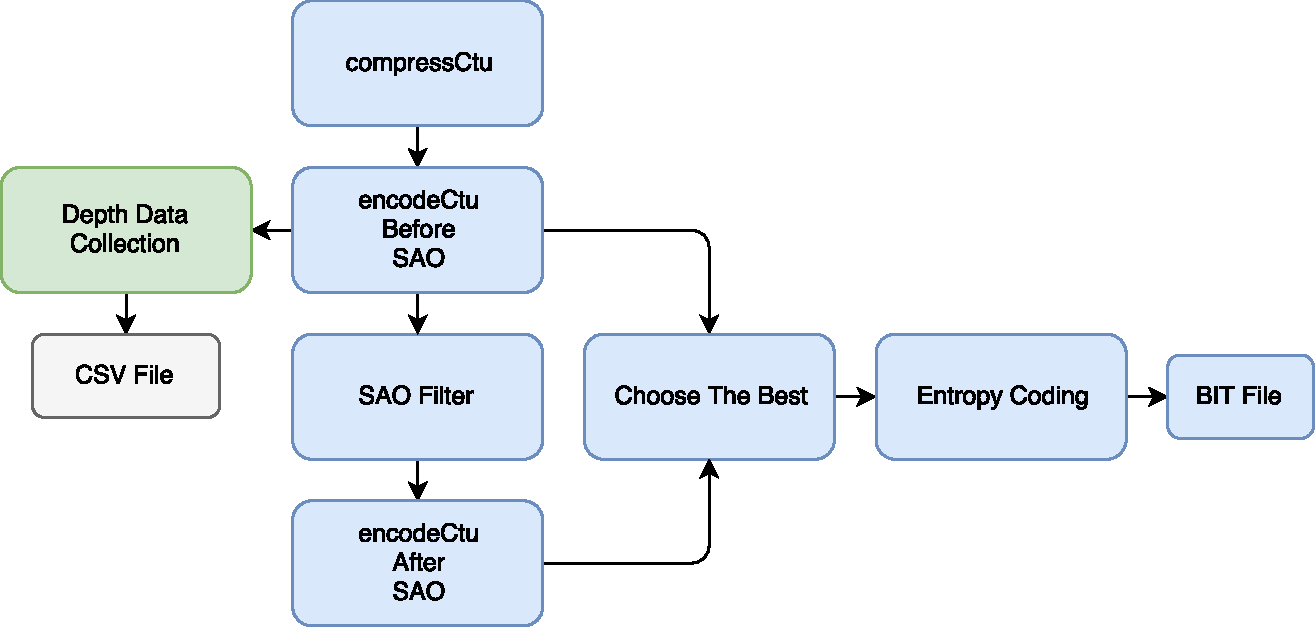
\includegraphics[width=\textwidth,height=\textheight,keepaspectratio]{Figures/thesis-data-collecting-diagram.pdf}
    \caption[Data collecting diagram]{Data collecting diagram.}
    \label{fig:data-collection-diagram}
\end{figure}
\begin{figure}
    \centering
    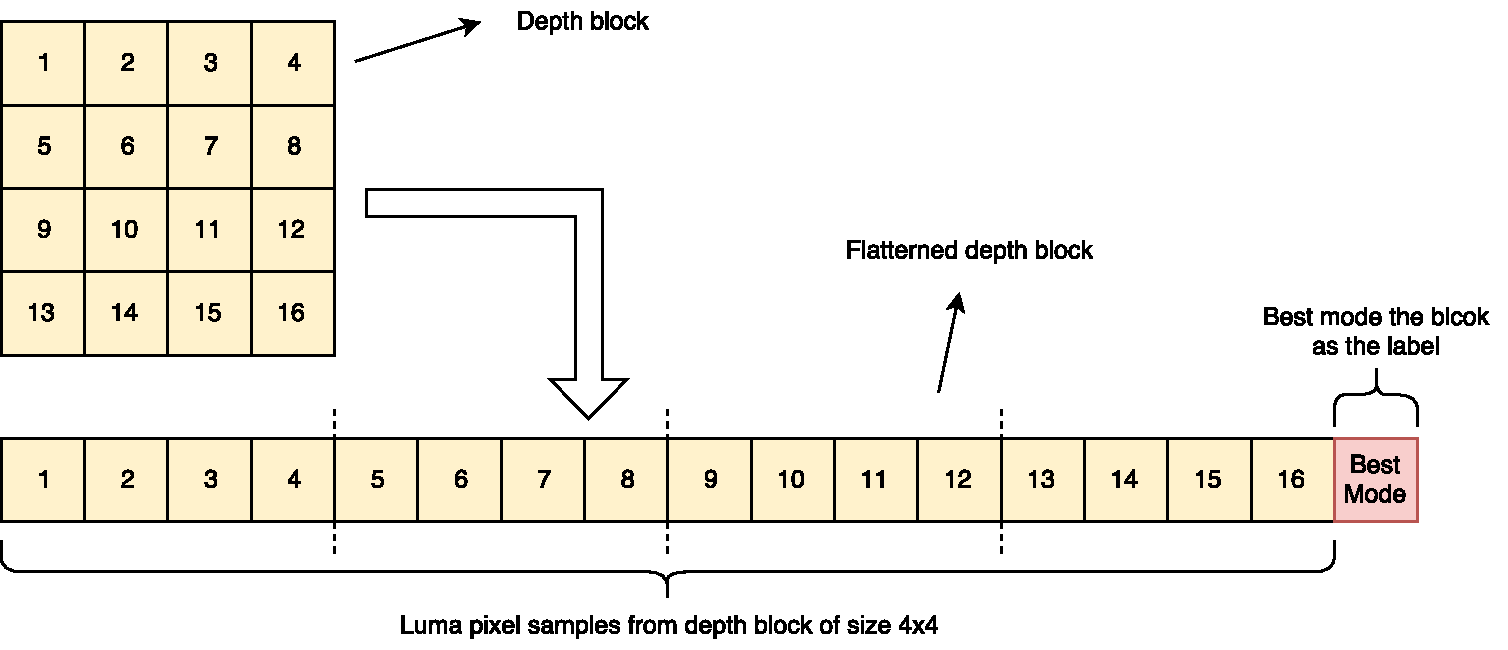
\includegraphics[width=\textwidth,height=\textheight,keepaspectratio]{Figures/flattern-pixels-into-single-line.pdf}
    \caption[Flatten Luma samples into one line and append best mode at the end]{Flatten Luma samples into one line and append best mode at the end.}\label{fig:flattern-data-into-one-dimension}
\end{figure}
During the data collecting process, only Luma samples in depth blocks
are used since we are trying to
reduce the computational complexity of depth map encoding.
As shown in Figure~\ref{fig:flattern-data-into-one-dimension} 
on page~\pageref{fig:flattern-data-into-one-dimension},
the Luma samples are flattened from rectangle CU blocks into
a single row which will be subsequently written into associated CSV file.

The detailed implementation for the module of \emph{depth data collection}
is shown in Algorithm~\ref{algo:collect-data} 
on page~\pageref{algo:collect-data}.
\begin{algorithm}[!b]
    \SetKwData{pcCU}{pcCU}
    \SetKwData{Left}{left}
    \SetKwData{uiAbsPartIdx}{uiAbsPartIdx}
    \SetKwData{uiDepth}{uiDepth}
    \SetKwData{DISFlag}{DISFlag}
    \SetKwData{iPartNum}{iPartNum}
    \SetKwData{sizeOfNByN}{sizeOfNByN}
    \SetKwData{maxCUWidth}{maxCUWidth}
    \SetKwData{pcPic}{pcPic}
    \SetKwData{pcSlice}{pcSlice}
    \SetKwData{pOrg}{pOrg}
    \SetKwData{iStride}{iStride}
    \SetKwData{uiCuSize}{uiCuSize}
    \SetKwData{pOrgPel}{pOrgPel}
    \SetKwData{sizeOfSubBlk}{sizeOfSubBlk}
    \SetKwData{uiTPelY}{uiTPelY}
    \SetKwData{uiLPelX}{uiLPelX}
    \SetKwData{yStartPos}{yStartPos}
    \SetKwData{yEndPos}{yEndPos}
    \SetKwData{xStartPos}{xStartPos}
    \SetKwData{xEndPos}{xEndPos}
    \SetKwData{iDir}{iDir}
    \SetKwData{partitionMode}{partitionMode}
    \SetKwFunction{getCUSize}{getCUSize}
    \SetKwFunction{getSizeOfSubBlk}{getSizeOfSubBlk}
    \SetKwFunction{FindCompress}{FindCompress}
    \SetKwFunction{getIntraDir}{getIntraDir}
    \SetKwFunction{getPic}{getPic}
    \SetKwFunction{getSlice}{getSlice}
    \SetKwFunction{getAddr}{getAddr}
    \SetKwFunction{getStride}{getStride}
    \SetKwFunction{getYPelCU}{getYPelCU}
    \SetKwFunction{getPartitionSize}{getPartitionSize}
    \DontPrintSemicolon % Some LaTeX compilers require you to use \dontprintsemicolon instead
    \KwIn{CU data structure \pcCU,
    absolute partition index of CU \uiAbsPartIdx,
    quad-tree depth \uiDepth}
    \KwOut{Flattened luma pixel values of each block together with
    the index of its best intra mode in each row of the output csv file}
    \Begin{
    \For{each CU in depth maps}{
    \uiCuSize$\leftarrow$\getCUSize{\pcCU, \uiDepth}\;
    \pOrgPel$\leftarrow$\getYPelCU{\pcCU}\;
    \If{\DISFlag $\equiv 0$}{
    %  \partitionMode$\leftarrow$ \getPartitionSize{$Im[i,j-1]$}\;
    \partitionMode$\leftarrow$\getPartitionSize{\pcCU, \uiAbsPartIdx}\;

    \eIf{\partitionMode $\equiv$ \sizeOfNByN}{
    \iPartNum$\leftarrow 4$\;
    }{
    \iPartNum$\leftarrow 1$\;
    }

    \For{$j\leftarrow 0$ \KwTo \iPartNum}{
    $iDir[j]$ $\leftarrow$ \getIntraDir{\pcCU, \uiAbsPartIdx}\;
    }
    \eIf{\iPartNum $\equiv 1$}{
    %      \tcc{collect luma values and the best mode for a single block}
    Create a new csv file, append the value of \uiDepth at the end of the name of the new csv file\;
    \For{$y\leftarrow 0$ \KwTo \uiCuSize}{
    \For{$x\leftarrow 0$ \KwTo \uiCuSize}{
    Write $pOrgPel[x]$ into $row_m$ in csv file\;
    }
    \pOrgPel $\leftarrow$ \pOrgPel + \iStride\;
    }
    Write $iDir[0]$ into the end of $row_m$ in the csv file\;
    }{
    %      \tcc{collect luma values and the best modes for each sub parts}
    Create a new csv file, append the value of (\uiDepth + $1$) at the end of the name of the new csv file\;
    \sizeOfSubBlk$\leftarrow$\getSizeOfSubBlk{\pcCU, \uiDepth}\;
    \For{$j\leftarrow 0$ \KwTo \iPartNum}{
    \uIf{$j\equiv0$}{
    \yStartPos $\leftarrow 0$
    \& \xStartPos $\leftarrow 0$
    \& \yEndPos $\leftarrow$ \sizeOfSubBlk\
    \& \xEndPos $\leftarrow$ \sizeOfSubBlk\;
    }
    \uElseIf{$j\equiv1$}{
    \yStartPos $\leftarrow 0$
    \& \xStartPos $\leftarrow$ \sizeOfSubBlk
    \& \yEndPos $\leftarrow$ \sizeOfSubBlk
    \& \xEndPos $\leftarrow \sizeOfSubBlk \times 2$\;
    }
    \uElseIf{$j\equiv2$}{
    \yStartPos $\leftarrow$ \sizeOfSubBlk
    \& \xStartPos $\leftarrow 0$
    \& \yEndPos $\leftarrow \sizeOfSubBlk \times 2$
    \& \xEndPos $\leftarrow$ \sizeOfSubBlk\;
    }
    \uElseIf{$j\equiv3$}{
    \yStartPos $\leftarrow$ \sizeOfSubBlk
    \& \xStartPos $\leftarrow$ \sizeOfSubBlk
    \& \yEndPos $\leftarrow \sizeOfSubBlk \times 2$
    \& \xEndPos $\leftarrow \sizeOfSubBlk \times 2$\;
    }
    }
    \For{$y\leftarrow$ \yStartPos \KwTo \yEndPos}{
    \For{$x\leftarrow$ \xStartPos \KwTo \xEndPos}{
    %   \For{$y\leftarrow 0$ \KwTo \yEndPos}{
    %        \For{$x\leftarrow 0$ \KwTo \xEndPos}{
    Write $pOrgPel[x]$ into $row_m$ in the csv file\;
    }
    \pOrgPel $\leftarrow$ \pOrgPel+ \iStride\;
    }
    Write $iDir[j]$ into the end of $row_m$ in the csv file\;
    }}}}
 \caption{Collect data}\label{algo:collect-data}
\end{algorithm}
The inputs (i.e., the CU data structure,
the absolute partition index and the corresponding quad-tree depth)
to the data collecting workflow are exactly the inputs to
the module of \emph{encodeCtu}.
Firstly, the partition mode of the CU, which can further indicate
the partition number to either be one or four, is obtained.
After that, 
% based on the partition number, the best modes, which are
% within the range of 0 (inclusive) to 36 (inclusive),
% are stored into an array of integer values.
if the partition number is equal to one, which means the current CU has not
been split and it has its own best mode, 
the luma pixel samples of this block are collected into a single row in the
CSV file.
In the end of the same row, the best mode of the CU is signaled;
else if the partition number is equal to four, which means the current CU has been
split to form four smaller sub-blocks with each sub-block has its
own best mode, the luma samples for each sub-block are collected into 
four different rows
in the CSV file with the last value in each row to be the best mode for each
sub-block.
\(HTM16.2\)~\parencite{RN214} is used in this work, which is the newest
version of the reference software of 3D-HEVC\@.
Considering we are focusing on the intra prediction,
All-Intra configuration is used.

\section{Data Visualization}\label{sec:data-visu}
Visualizing data is a good way for human to better understand
and memorize information. 
Complicated patterns hidden in the data are easier to be discovered when they 
are aesthetically presented via the graphical format.
% We visualize the collected data to understand them
% more clearly.
The collected data are visualized with the hope of
discovering more information from them.
% They shall be sufficient to support the discussions which are
% ;Showing visualizations for four sets of 
% Due to the large quantity of the data from the visualization perspective,
% based on the observations.
Discussions based on the observations of visualized blocks,
which have convinced us of the necessity of data 
pre-processing in Section~\ref{sec:data-preprocessing} before 
training the deep models, are given.

\subsection{Visualized Data}\label{subsec:see-data-visu}
We have four sets of data which are from blocks of size
\(4\times4\), \(8\times8\), \(16\times16\) and \(32\times32\).
% However, only the part of the visualization for data of block 
% size \(8\\times8\) are presented in this section due to the 
% below considerations:
The intra prediction modes in 3D-HEVC include
DC mode, PLANAR mode, 33 angular modes, DMM1 and DMM4.
In this thesis, several indices are assigned to each mode:
0 for DC mode, 1 for PLANAR mode, {[2,34]} for 33 angular modes, 35
for DMM1 and 36 for DMM4.

After all the four sets of data have been visualized,
it is found that four corresponding sets of visualizations
give same hints which are discussed in
Subsection~\ref{subsec:discussion-about-data-visu}.
For this reason, only the visualizations of blocks of size \(8\times8\)
are shown.
There are totally 37 visualizations presented,
from Figure~\ref{fig:size8_mode0}, Figure~\ref{fig:size8_mode1},
\ldots to Figure~\ref{fig:size8_mode36}.

\begin{figure}[H]
    
        \vspace*{1cm} % vertical separation
    
        \begin{minipage}{0.49\textwidth}
            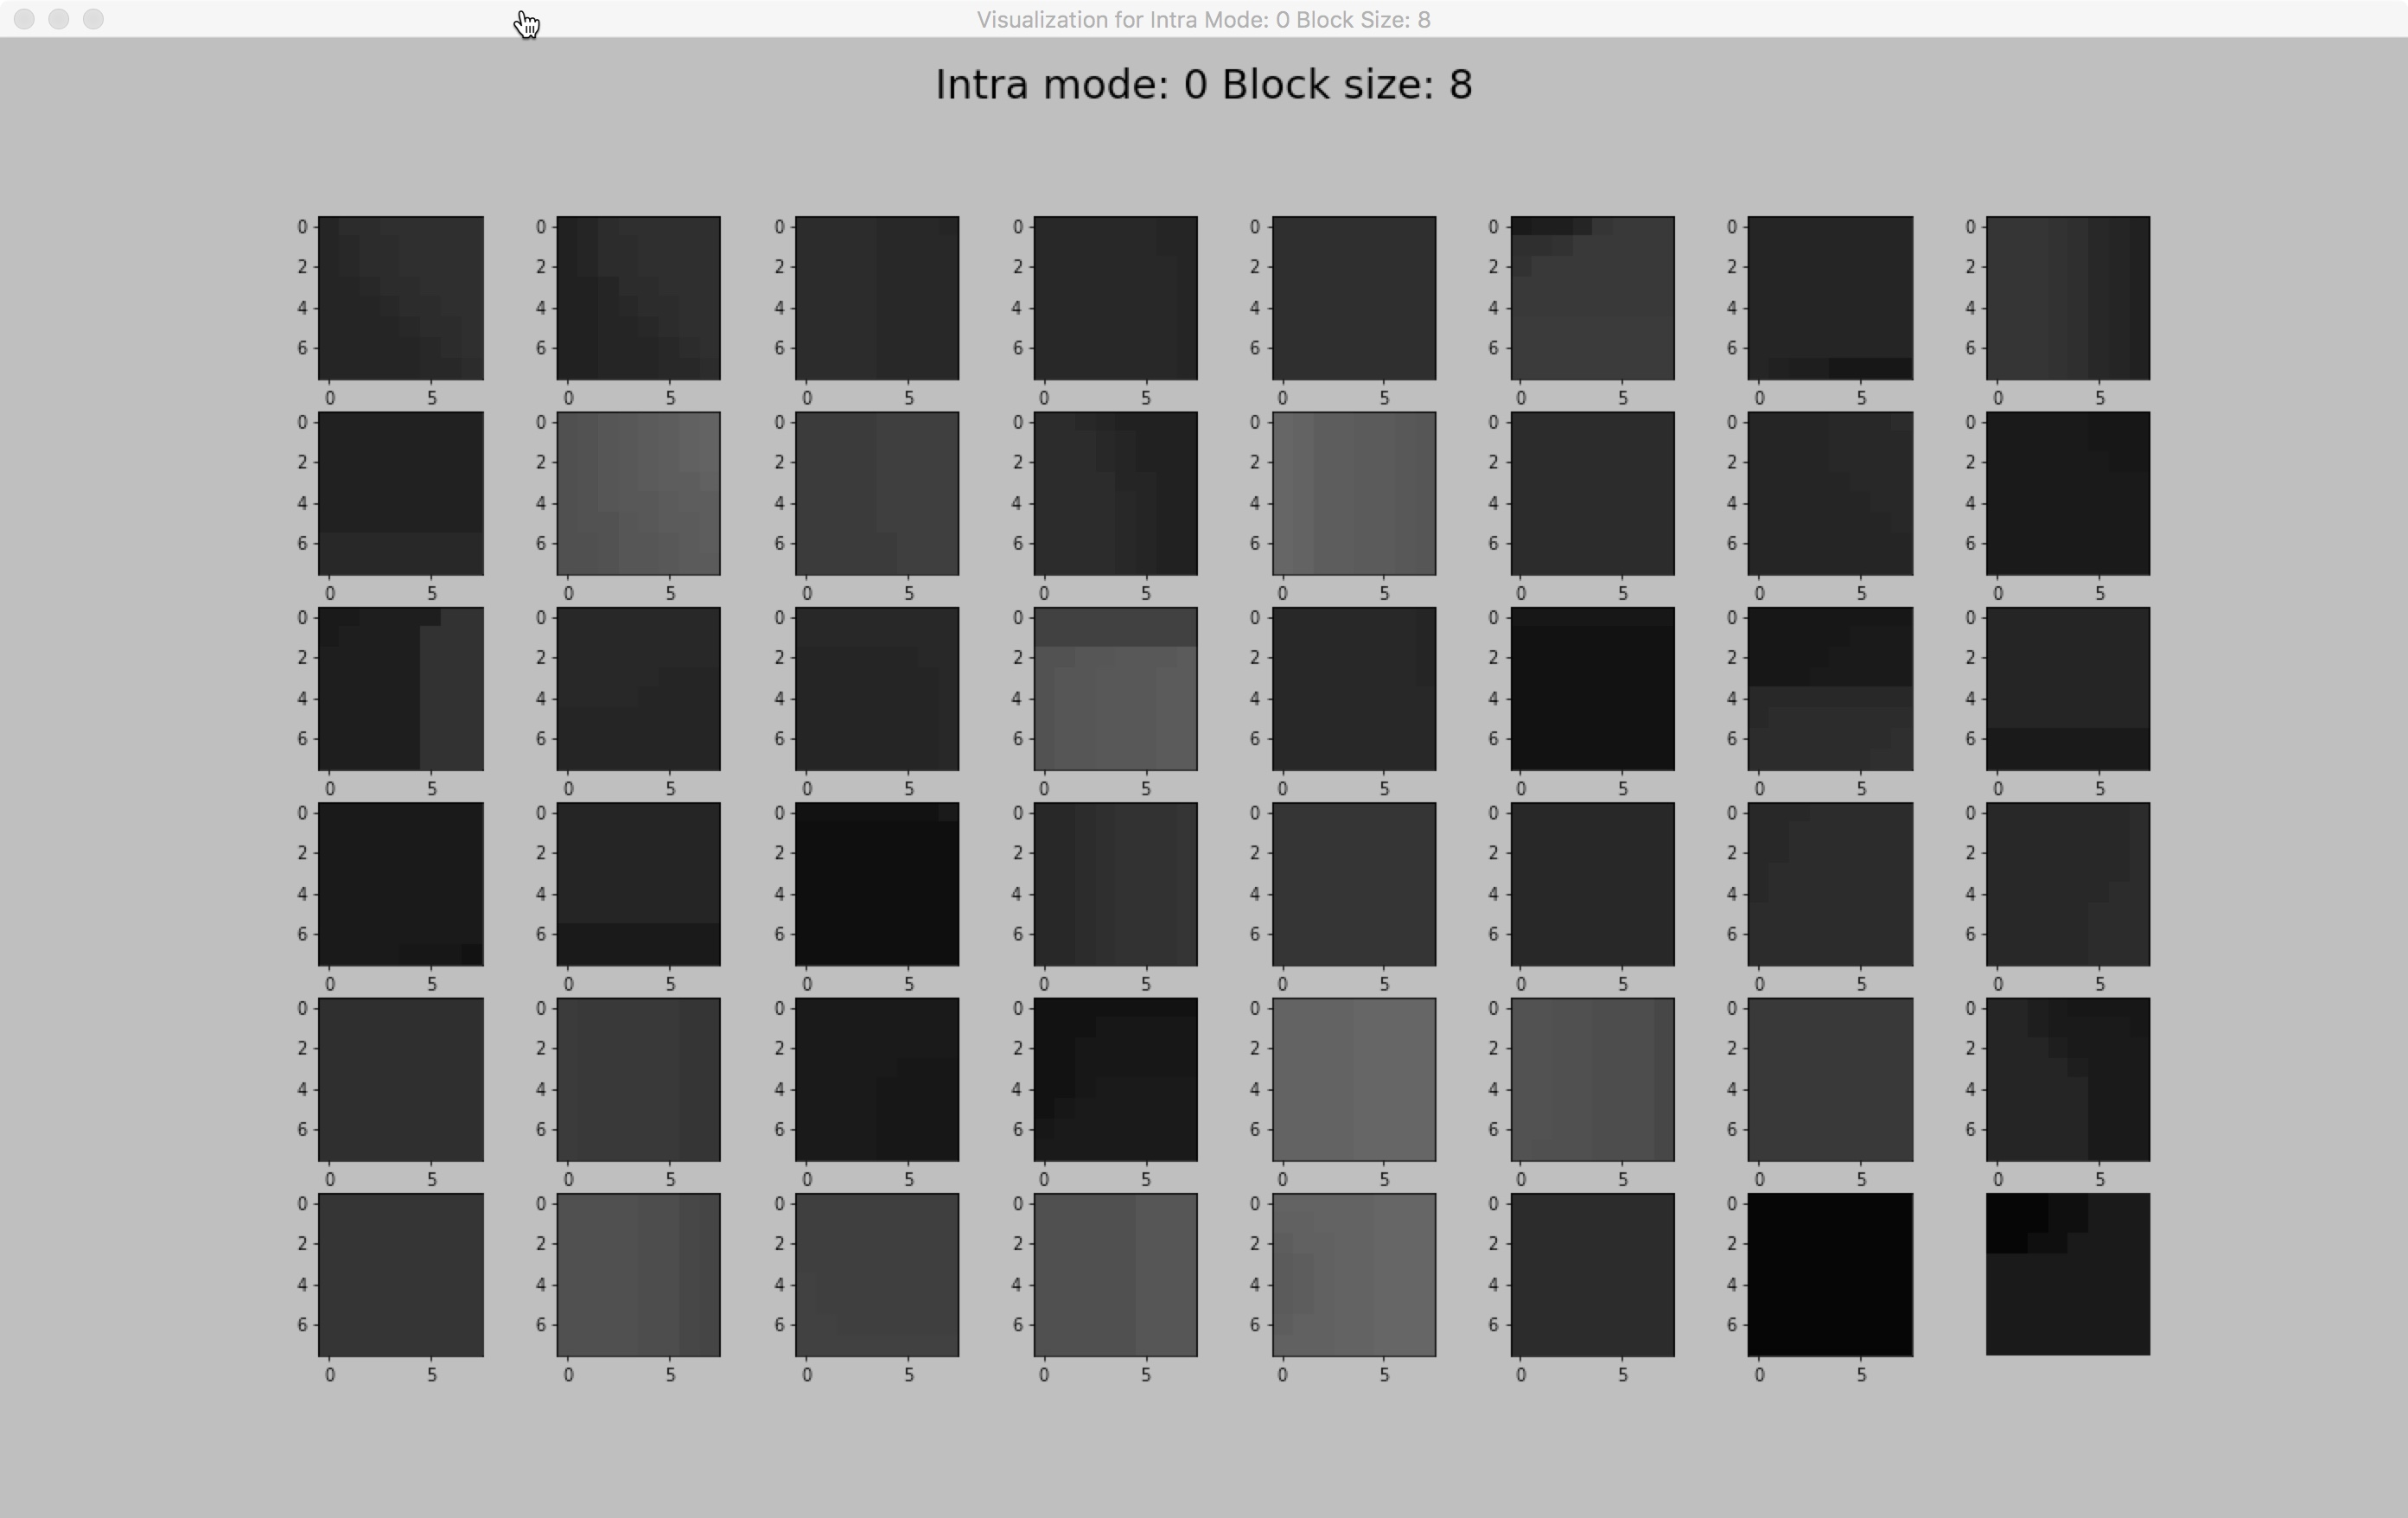
\includegraphics[width=\linewidth]{Figures/visu-size8x8/8-0}
            \caption[Visualizations for blocks tagged with intra DC]{Visualizations for blocks tagged with intra DC.}
            \label{fig:size8_mode0}
        \end{minipage}
        \hspace{\fill} % note: no blank line here
        \begin{minipage}{0.49\textwidth}
            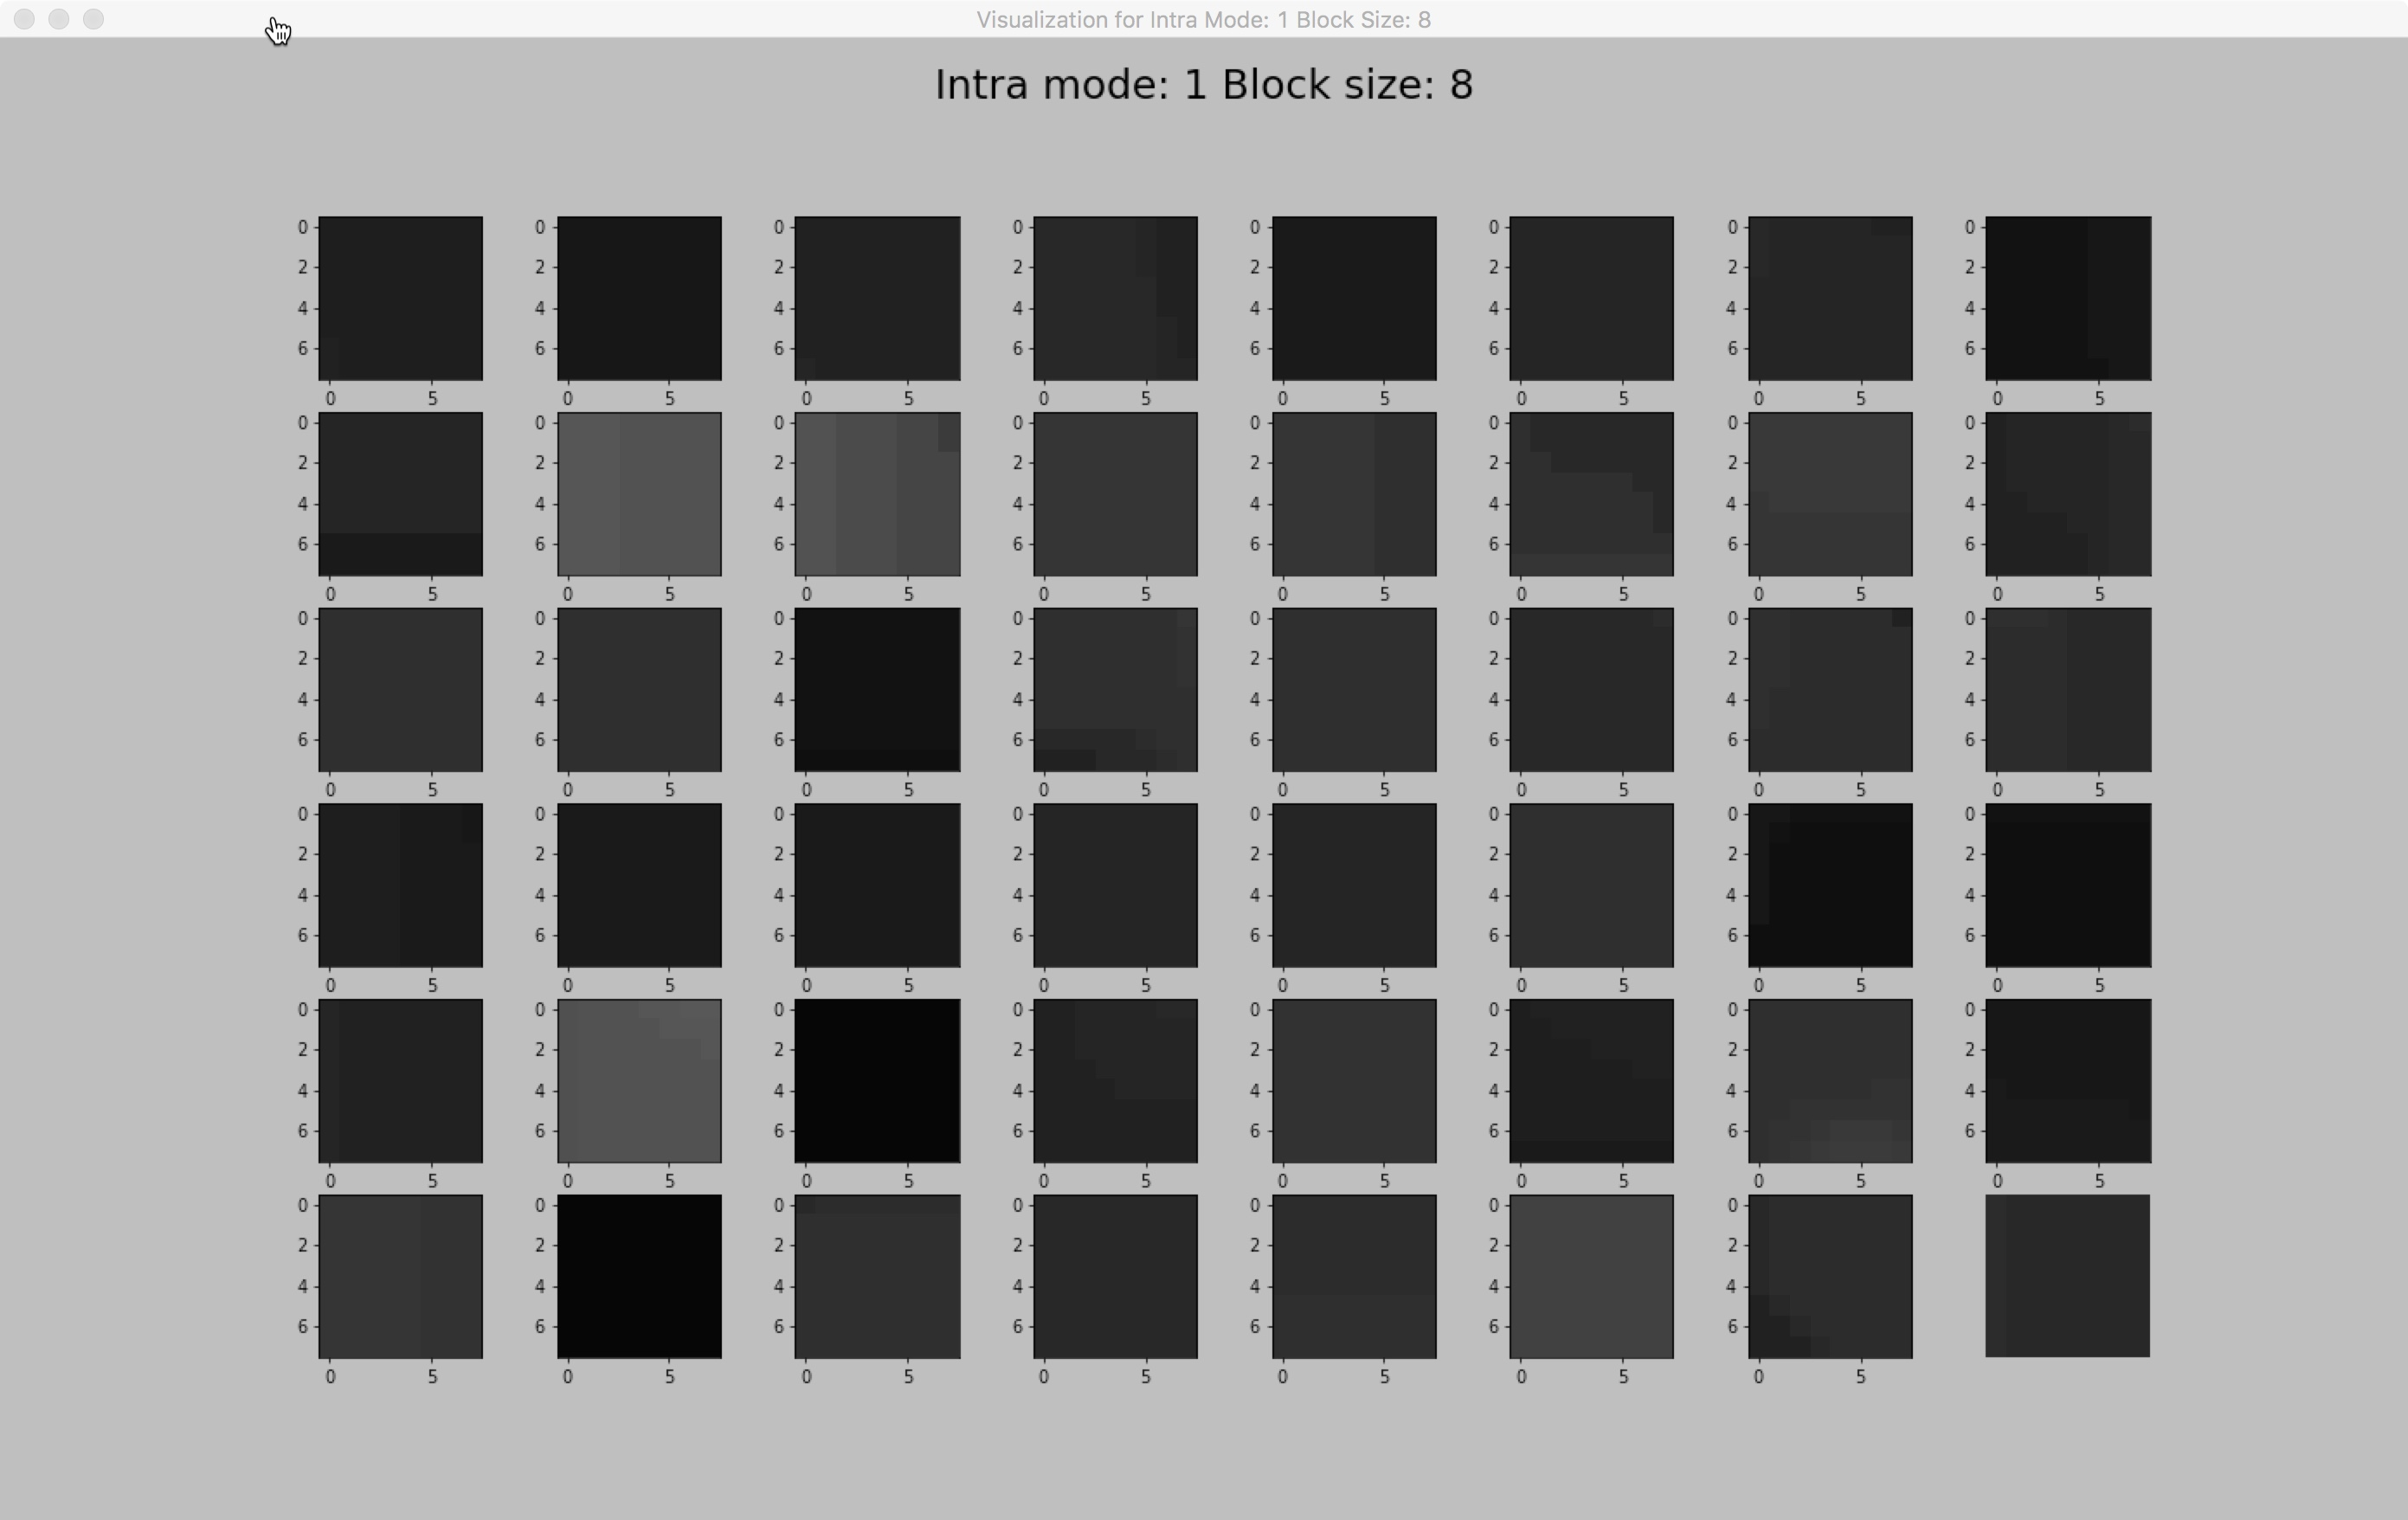
\includegraphics[width=\linewidth]{Figures/visu-size8x8/8-1}
            \caption[Visualizations for blocks tagged with intra PLANAR]{Visualizations for blocks tagged with intra PLANAR.}
            \label{fig:size8_mode1}
        \end{minipage}
        
        \vspace*{1cm} % vertical separation
    
        \begin{minipage}{0.49\textwidth}
            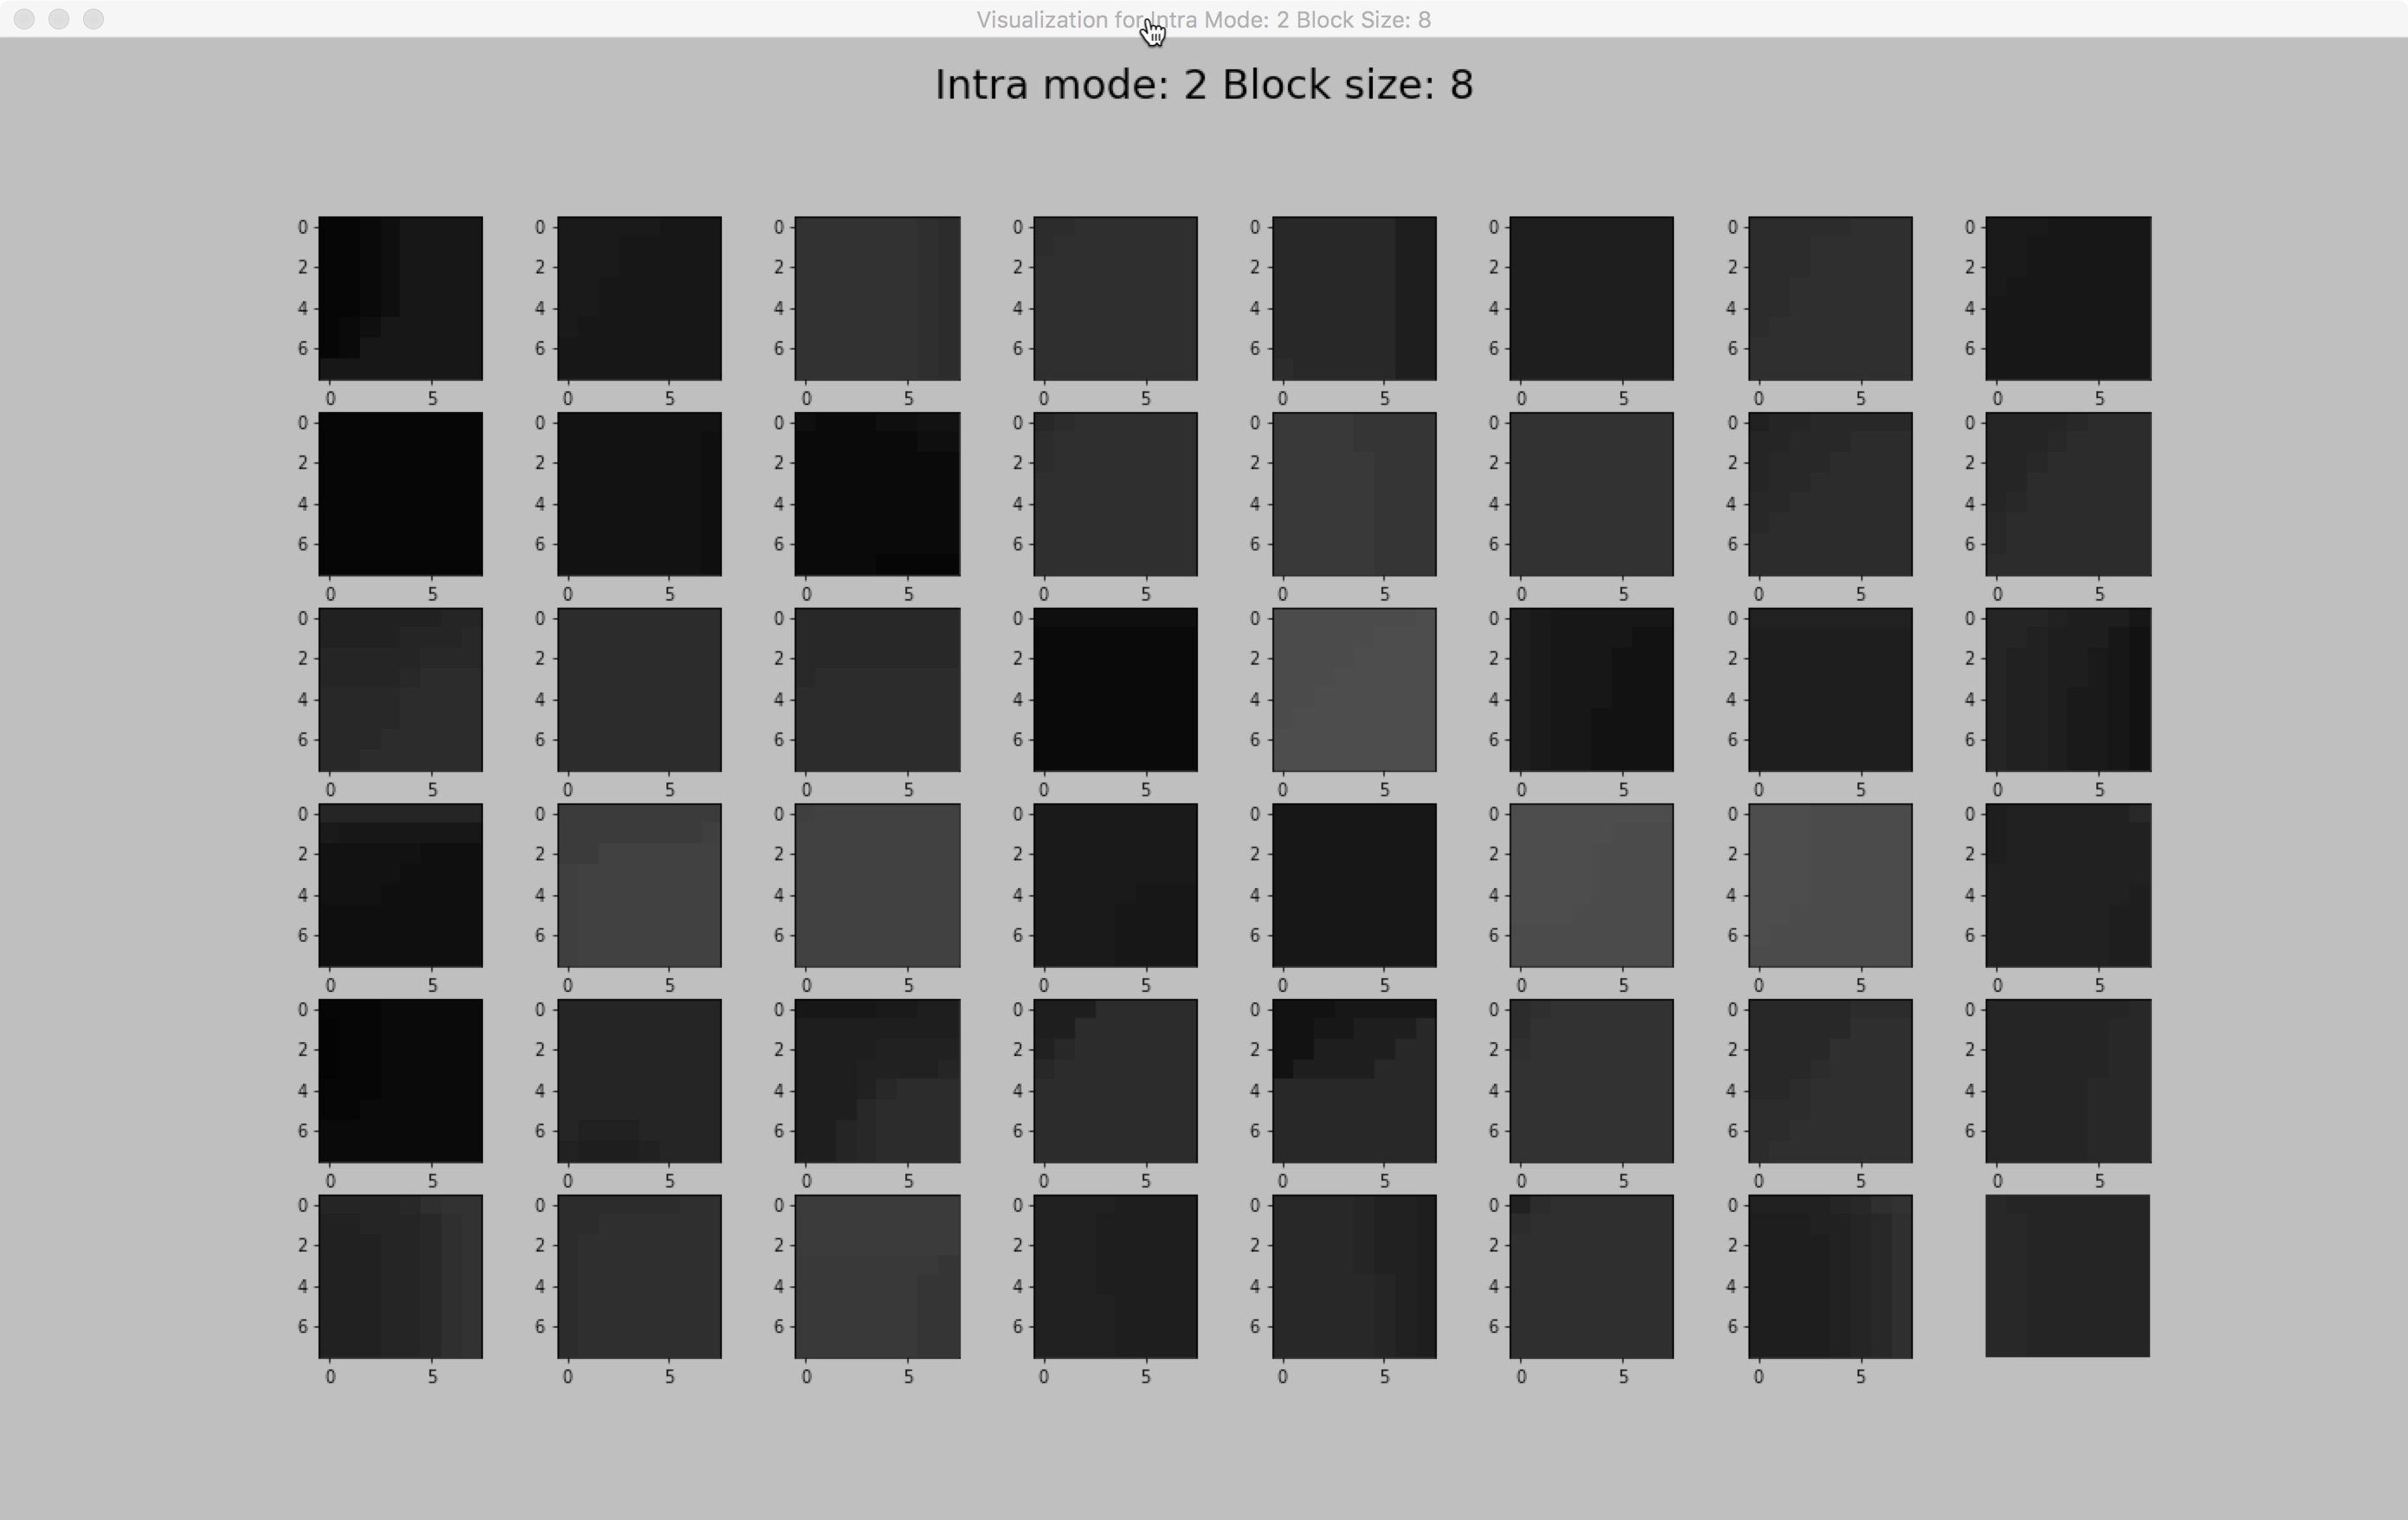
\includegraphics[width=\linewidth]{Figures/visu-size8x8/8-2.jpeg}
            \caption[Visualizations for blocks tagged with intra mode 2]{Visualizations for blocks tagged with intra mode 2.}
            \label{fig:size8_mode2}
        \end{minipage}
        \hspace{\fill} % note: no blank line here
        \begin{minipage}{0.49\textwidth}
            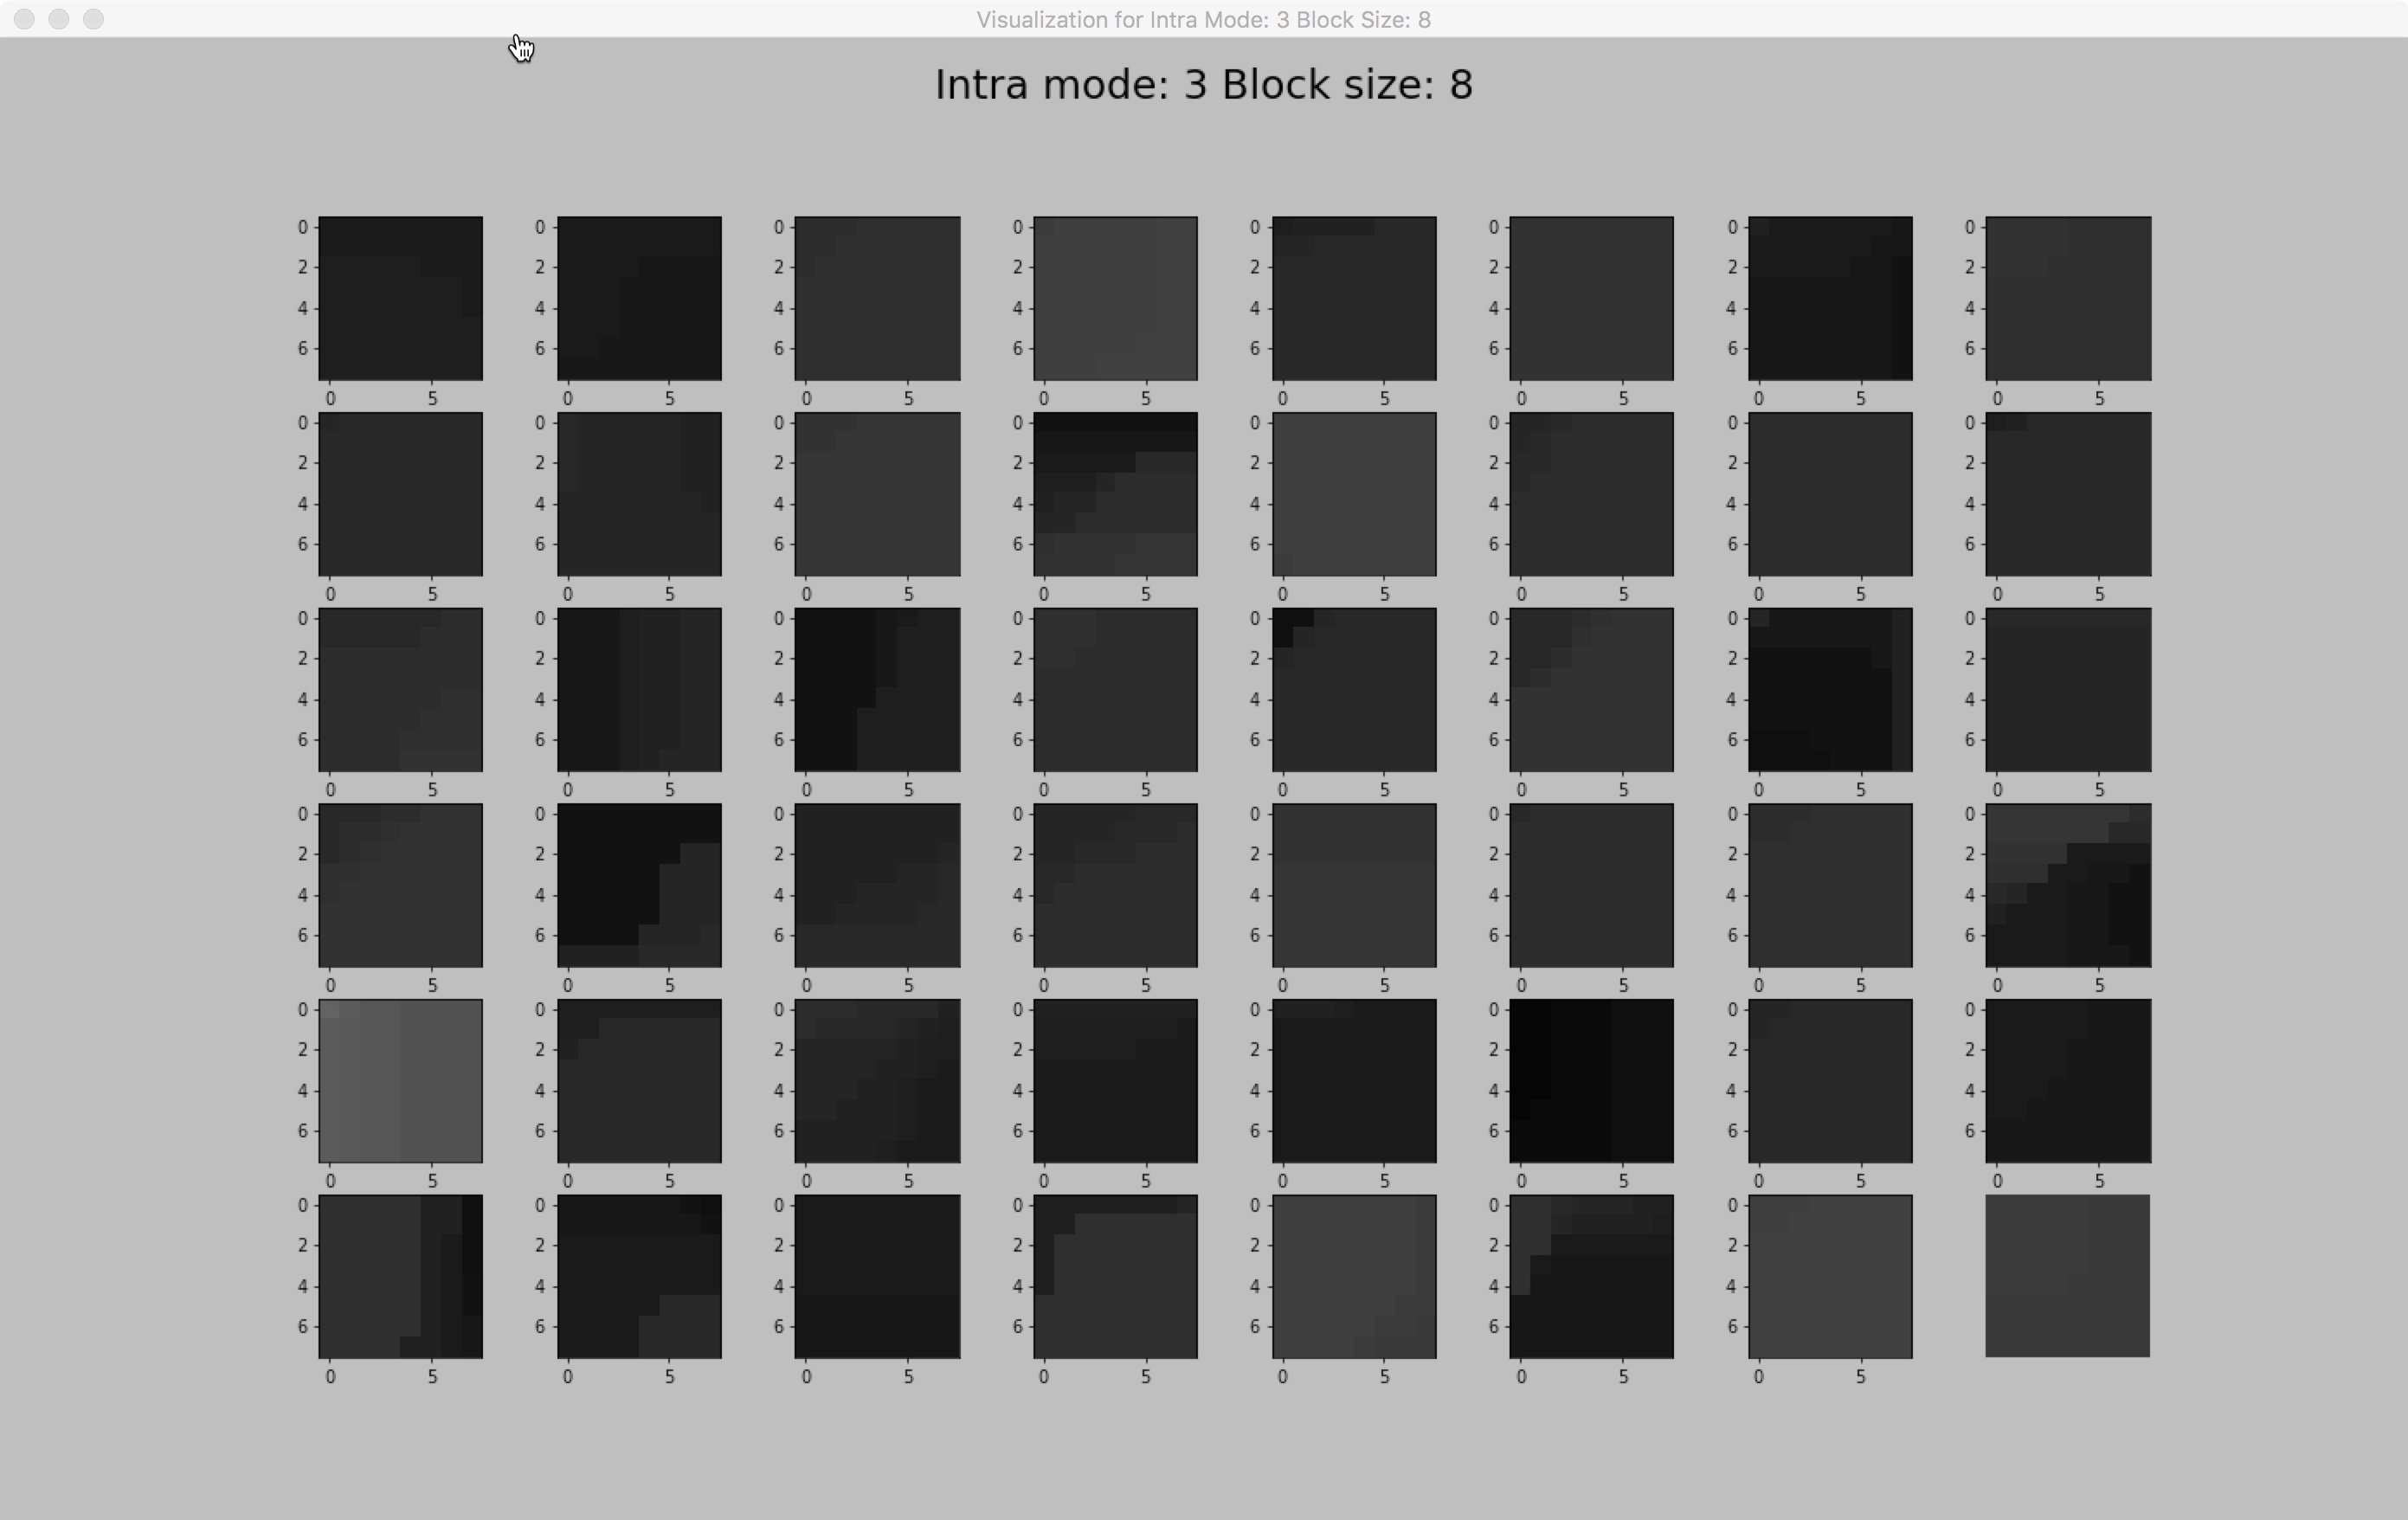
\includegraphics[width=\linewidth]{Figures/visu-size8x8/8-3}
            \caption[Visualizations for blocks tagged with intra mode 3]{Visualizations for blocks tagged with intra mode 3.}
            \label{fig:size8_mode3}
        \end{minipage}
    \end{figure}
    
    \begin{figure}
    
        \vspace*{1cm} % vertical separation
        
        \begin{minipage}{0.49\textwidth}
            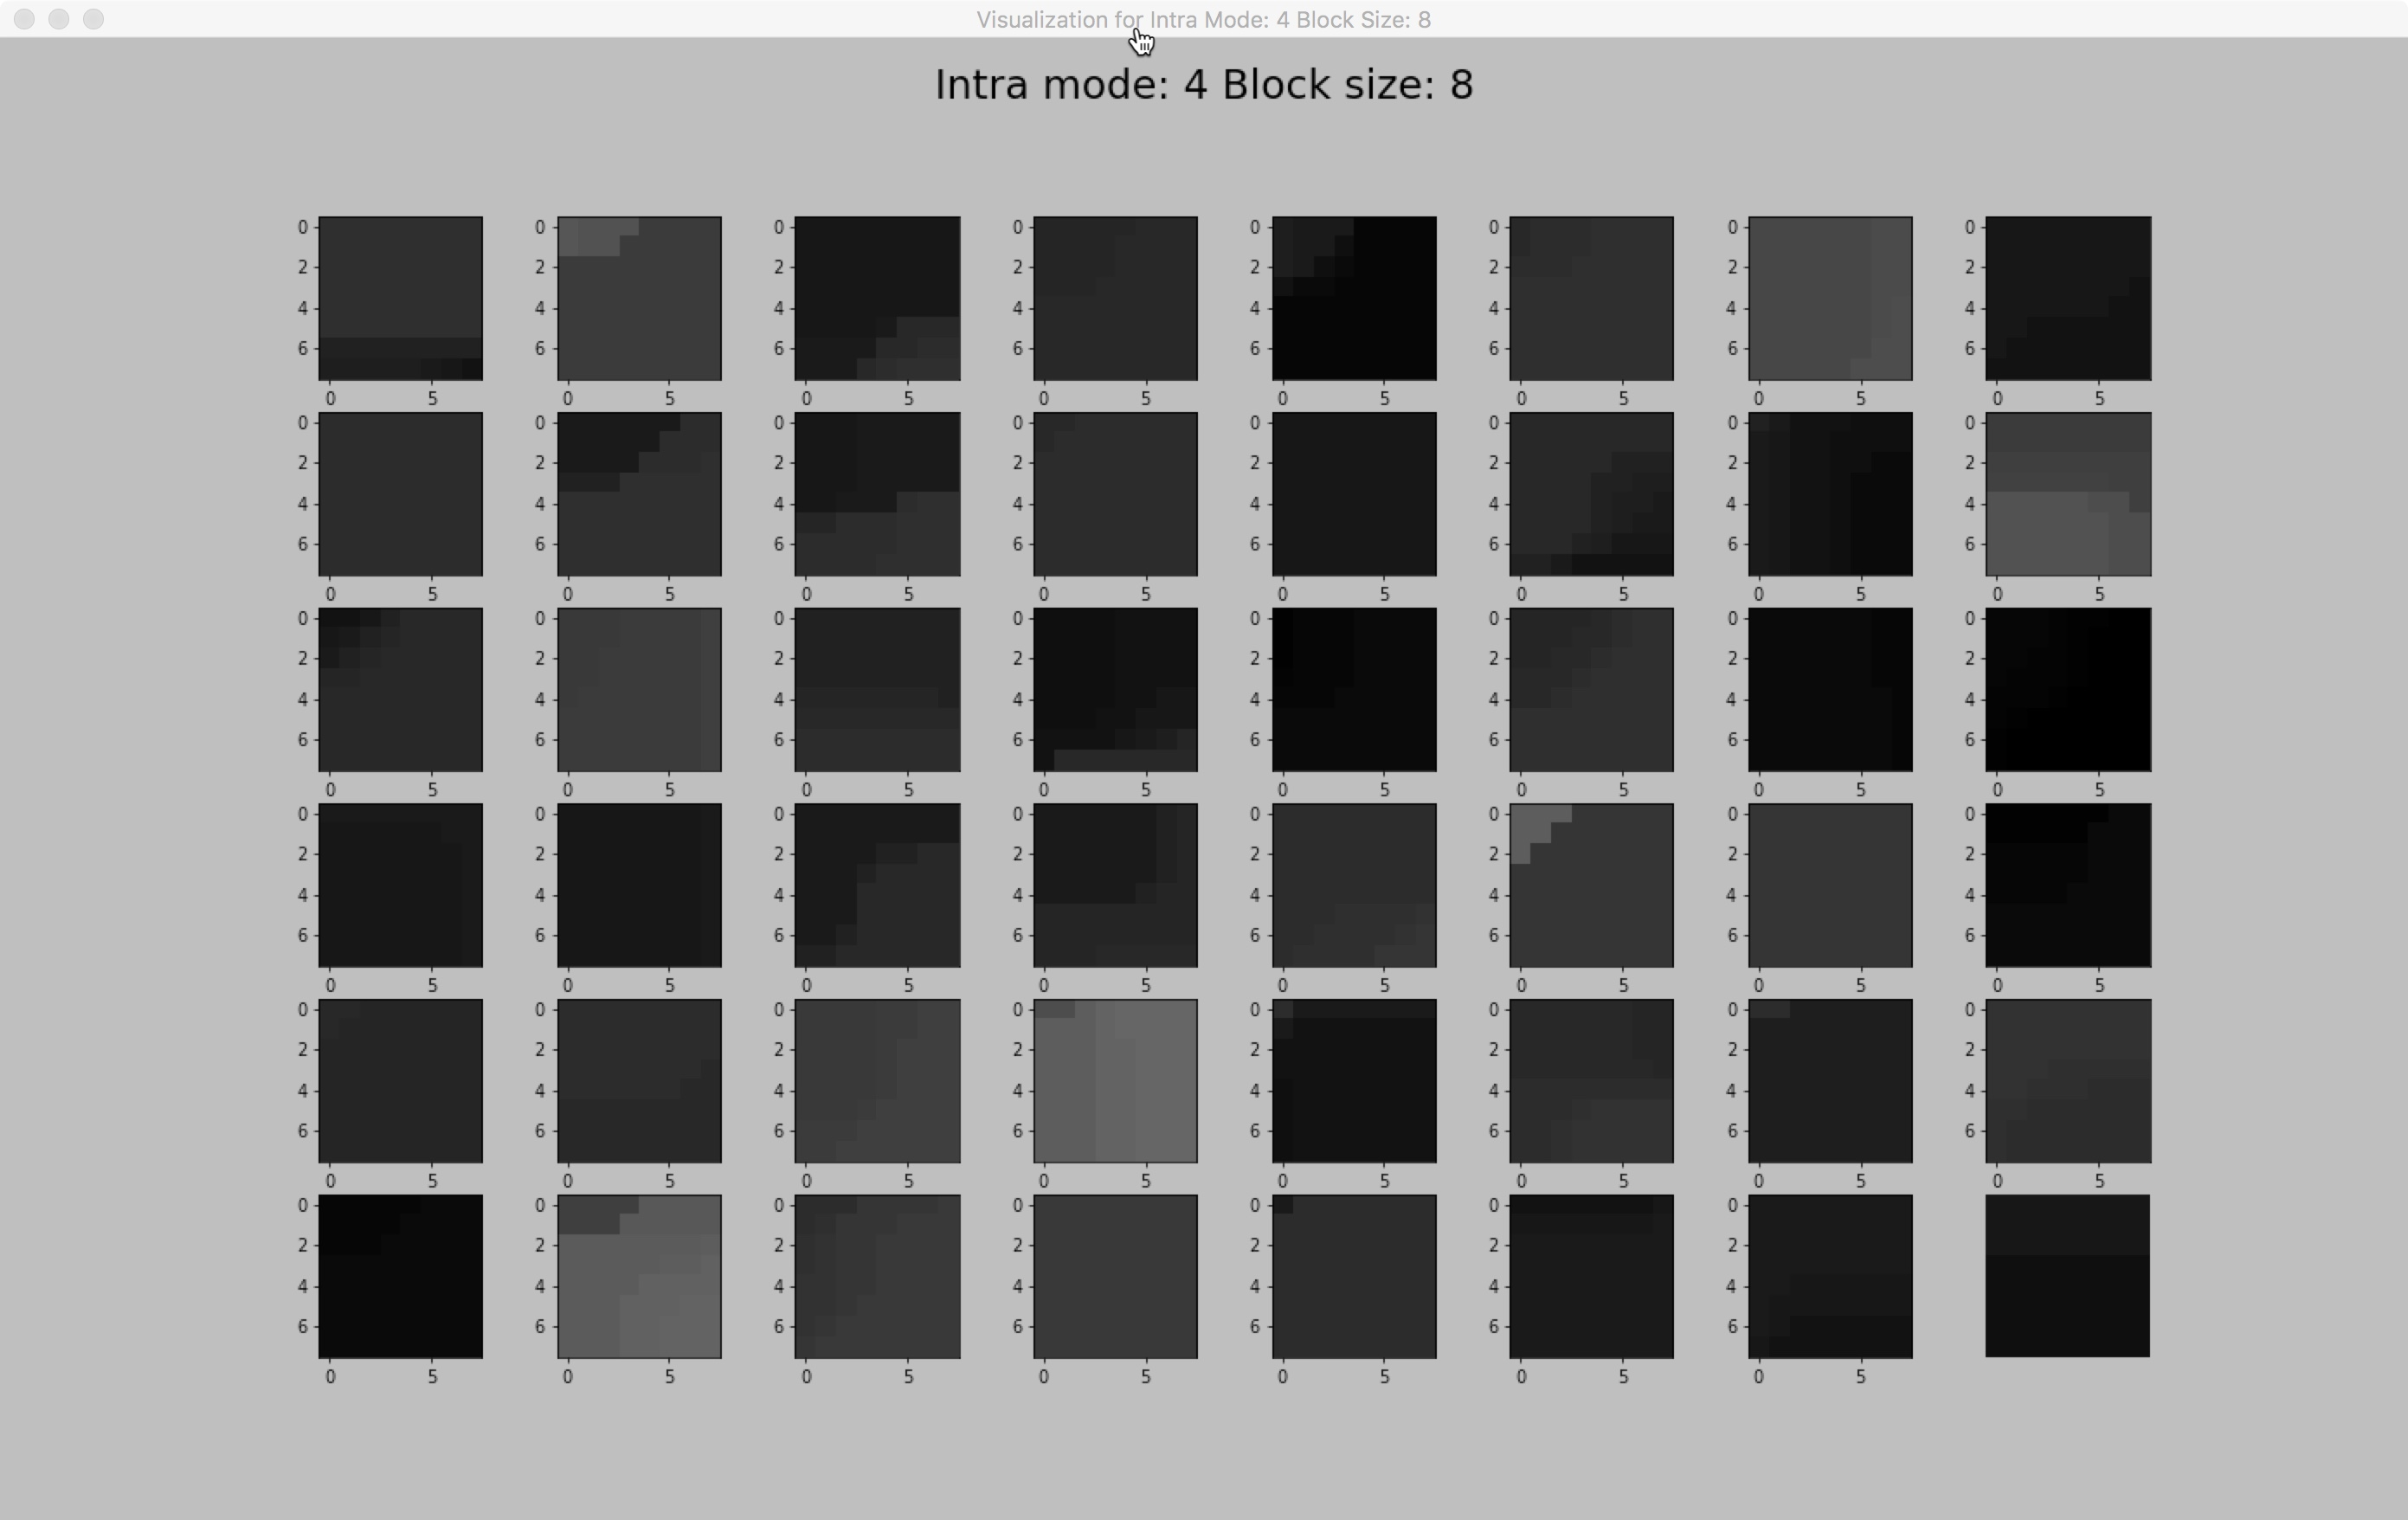
\includegraphics[width=\linewidth]{Figures/visu-size8x8/8-4}
            \caption[Visualizations for blocks tagged with intra mode 4]{Visualizations for blocks tagged with intra mode 4.}
            \label{fig:size8_mode4}
        \end{minipage}
        \hspace{\fill} % note: no blank line here
        \begin{minipage}{0.49\textwidth}
            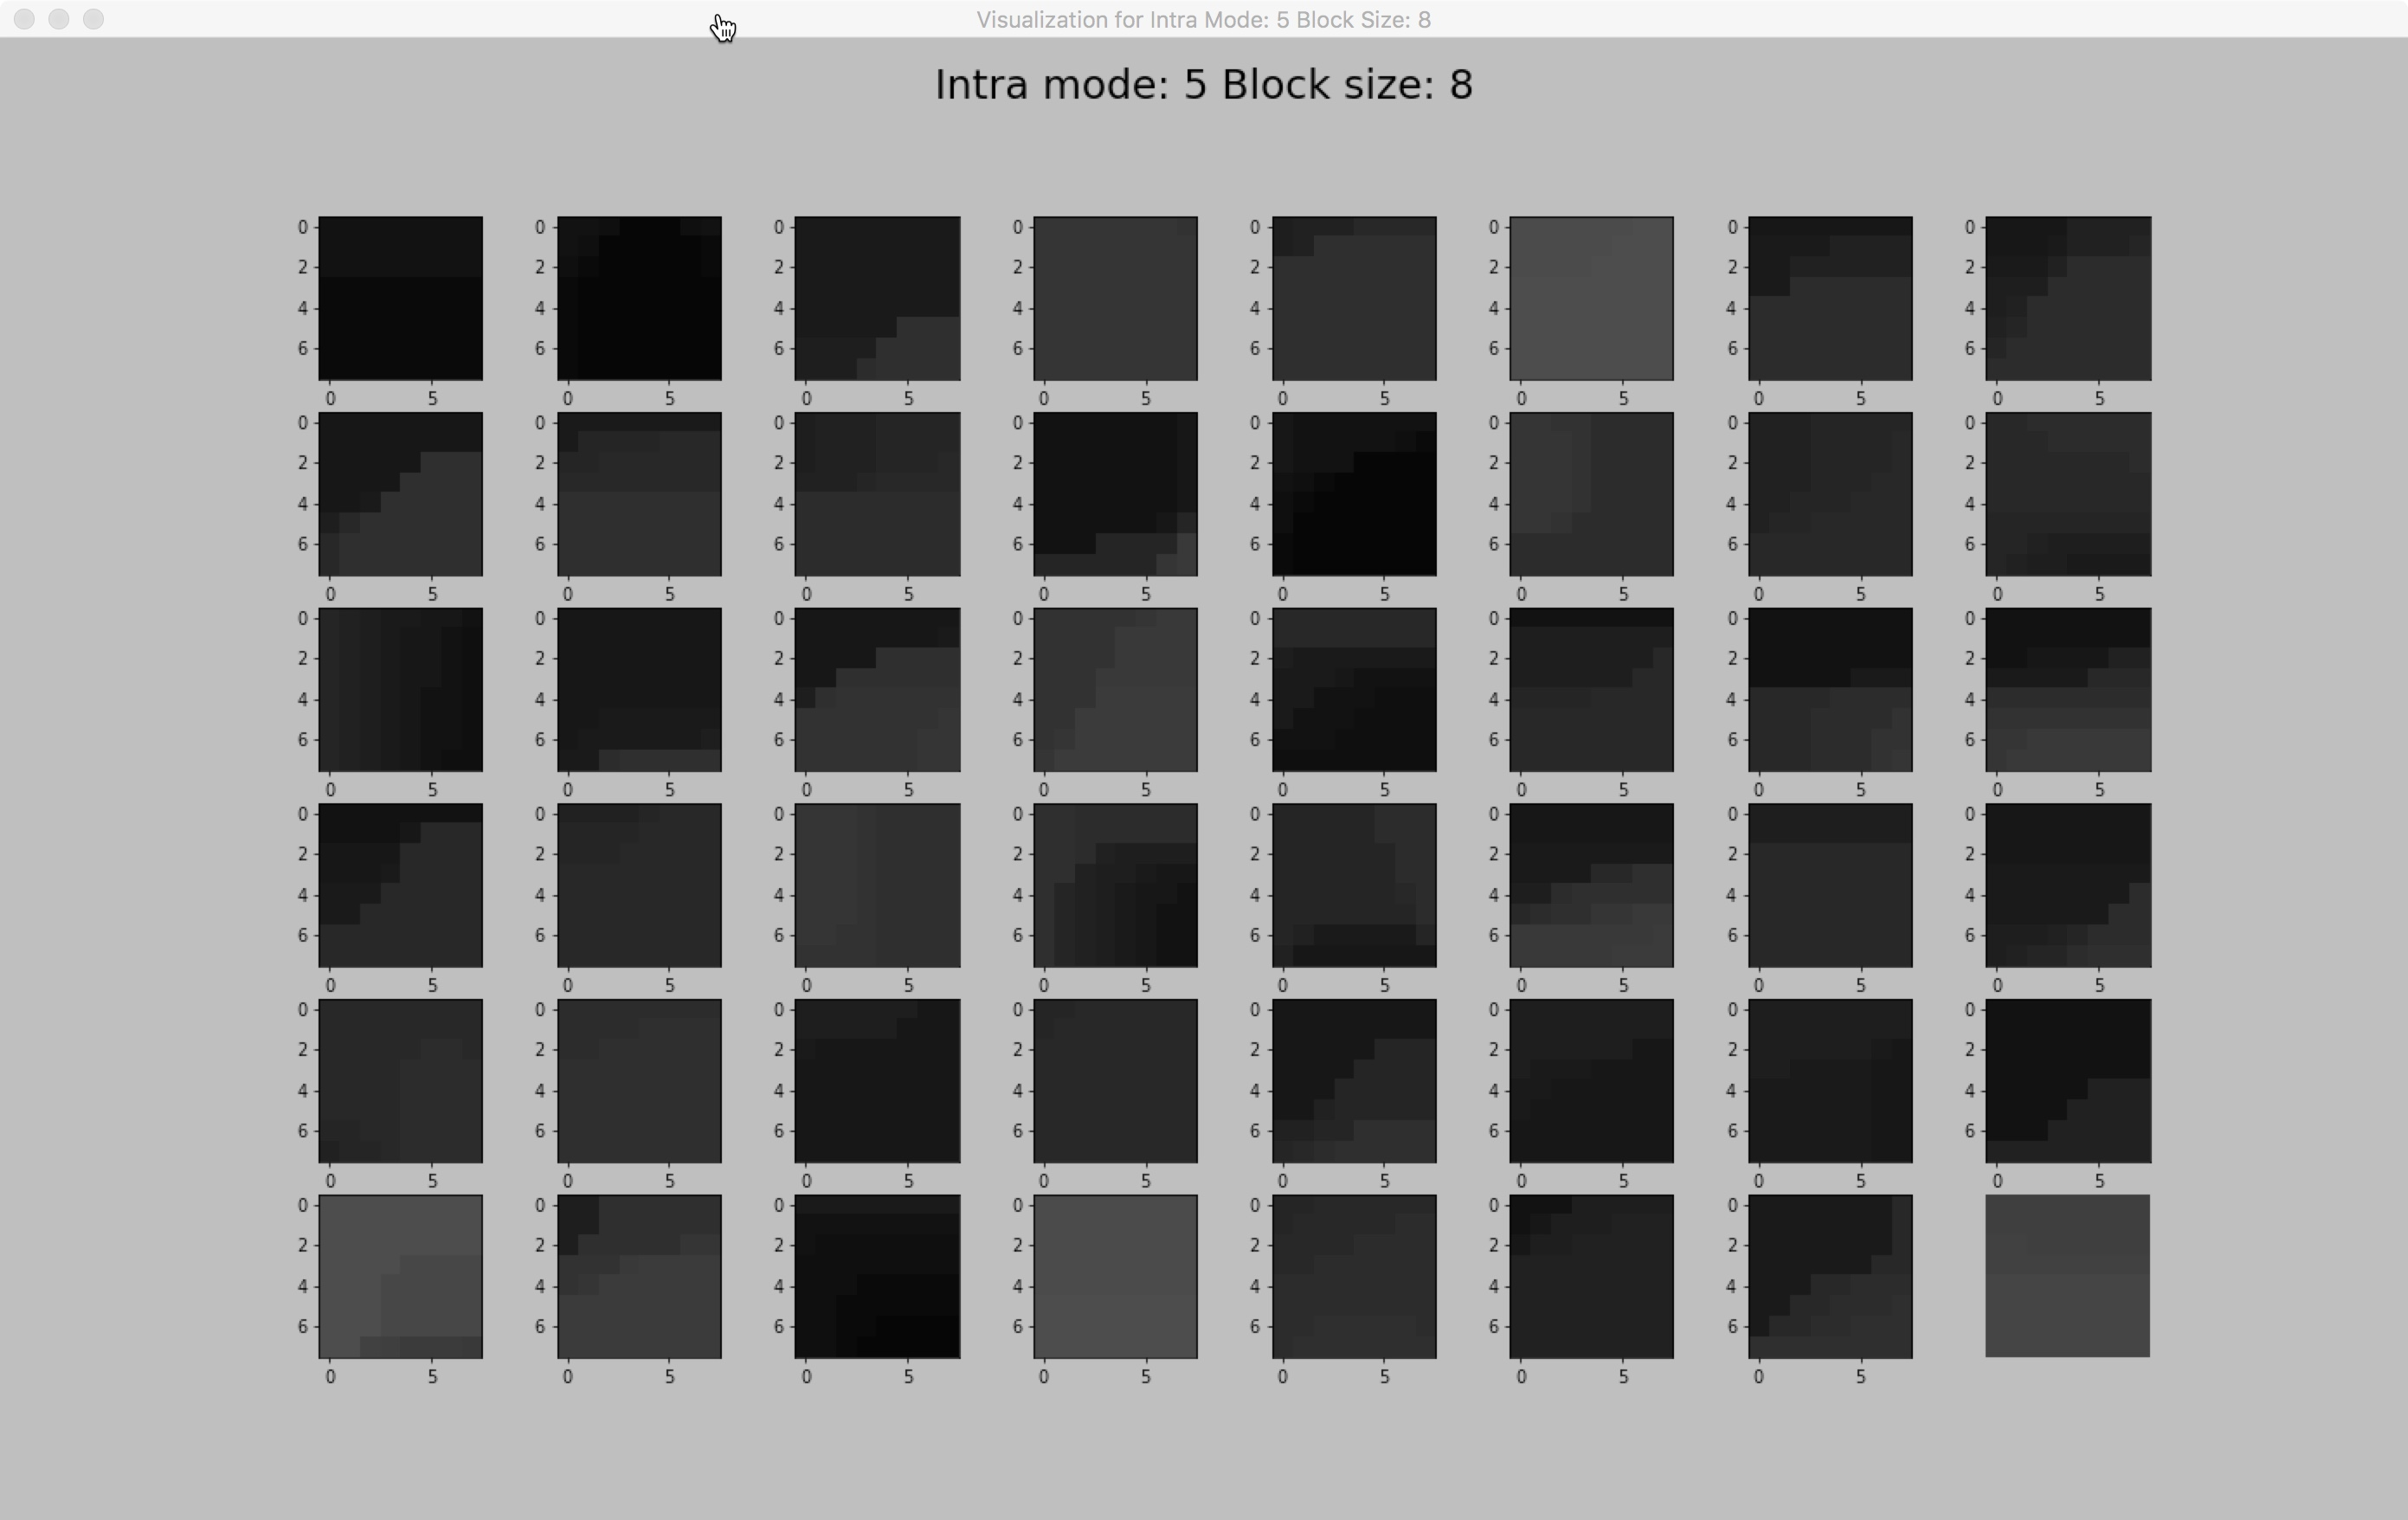
\includegraphics[width=\linewidth]{Figures/visu-size8x8/8-5}
            \caption[Visualizations for blocks tagged with intra mode 5]{Visualizations for blocks tagged with intra mode 5.}
            \label{fig:size8_mode5}
        \end{minipage}
    
        \vspace*{1cm} % vertical separation
    
        \begin{minipage}{0.49\textwidth}
            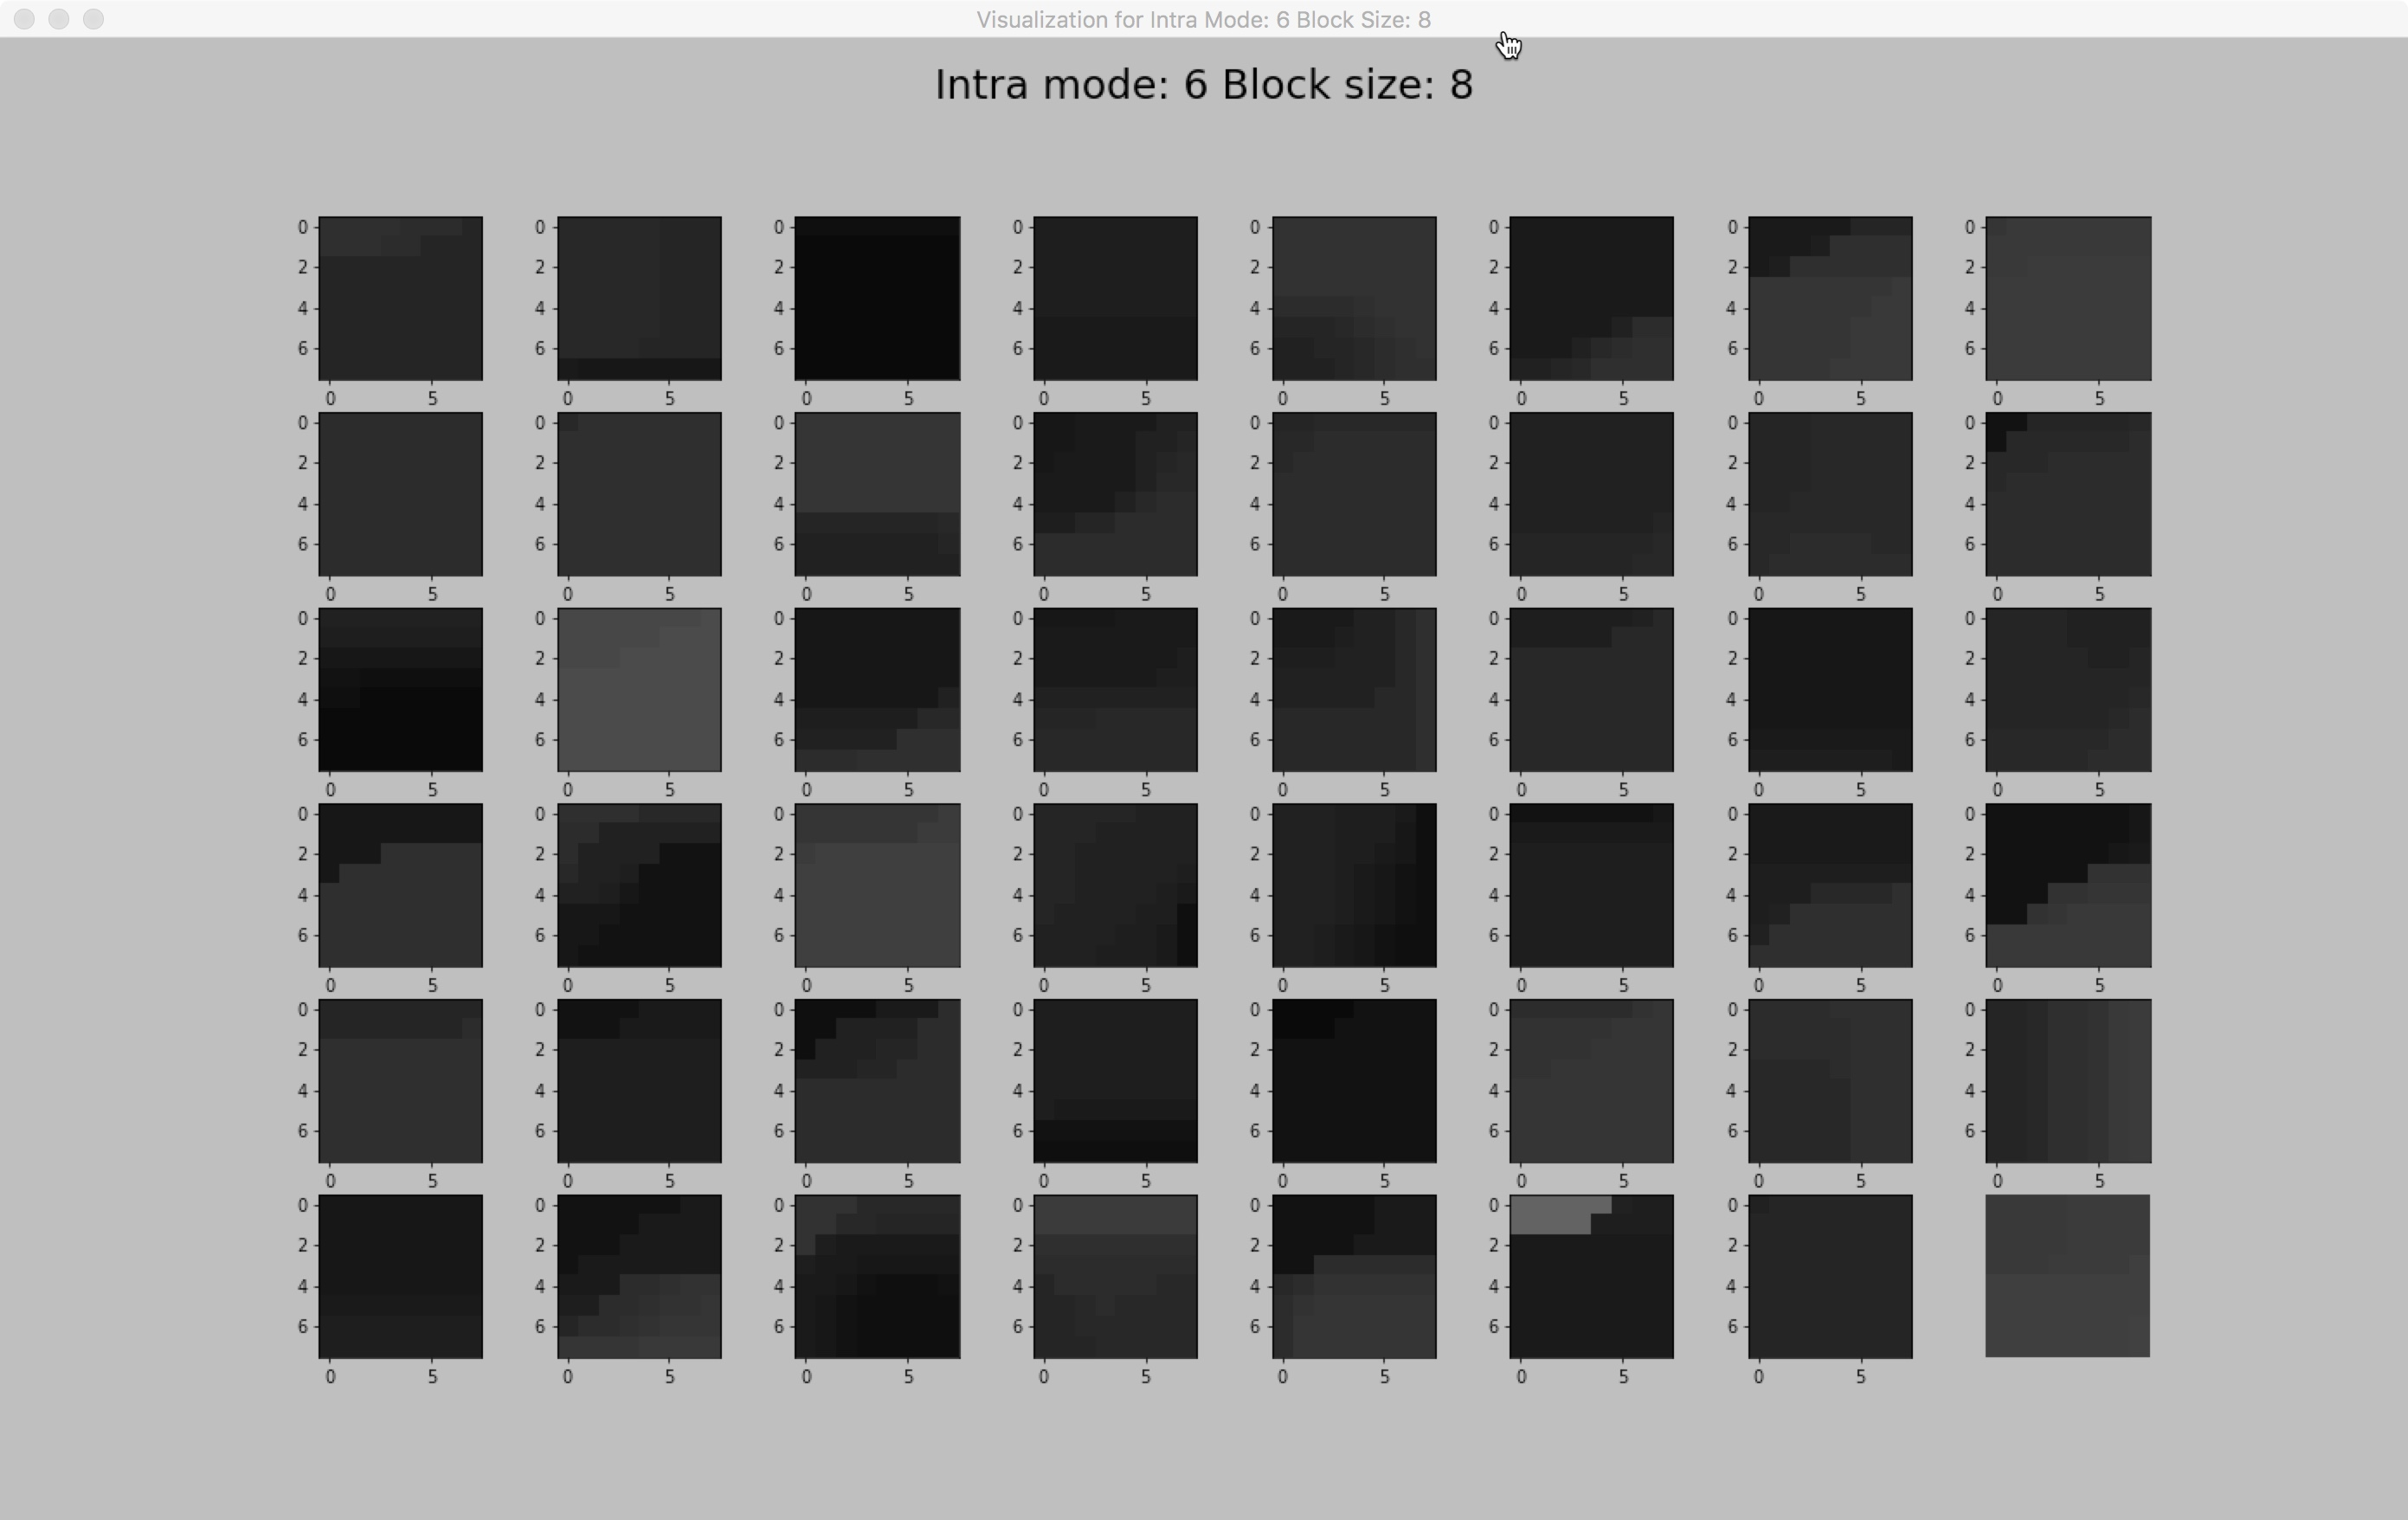
\includegraphics[width=\linewidth]{Figures/visu-size8x8/8-6}
            \caption[Visualizations for blocks tagged with intra mode 6]{Visualizations for blocks tagged with intra mode 6.}
            \label{fig:size8_mode6}
        \end{minipage}
        \hspace{\fill} % note: no blank line here
        \begin{minipage}{0.49\textwidth}
            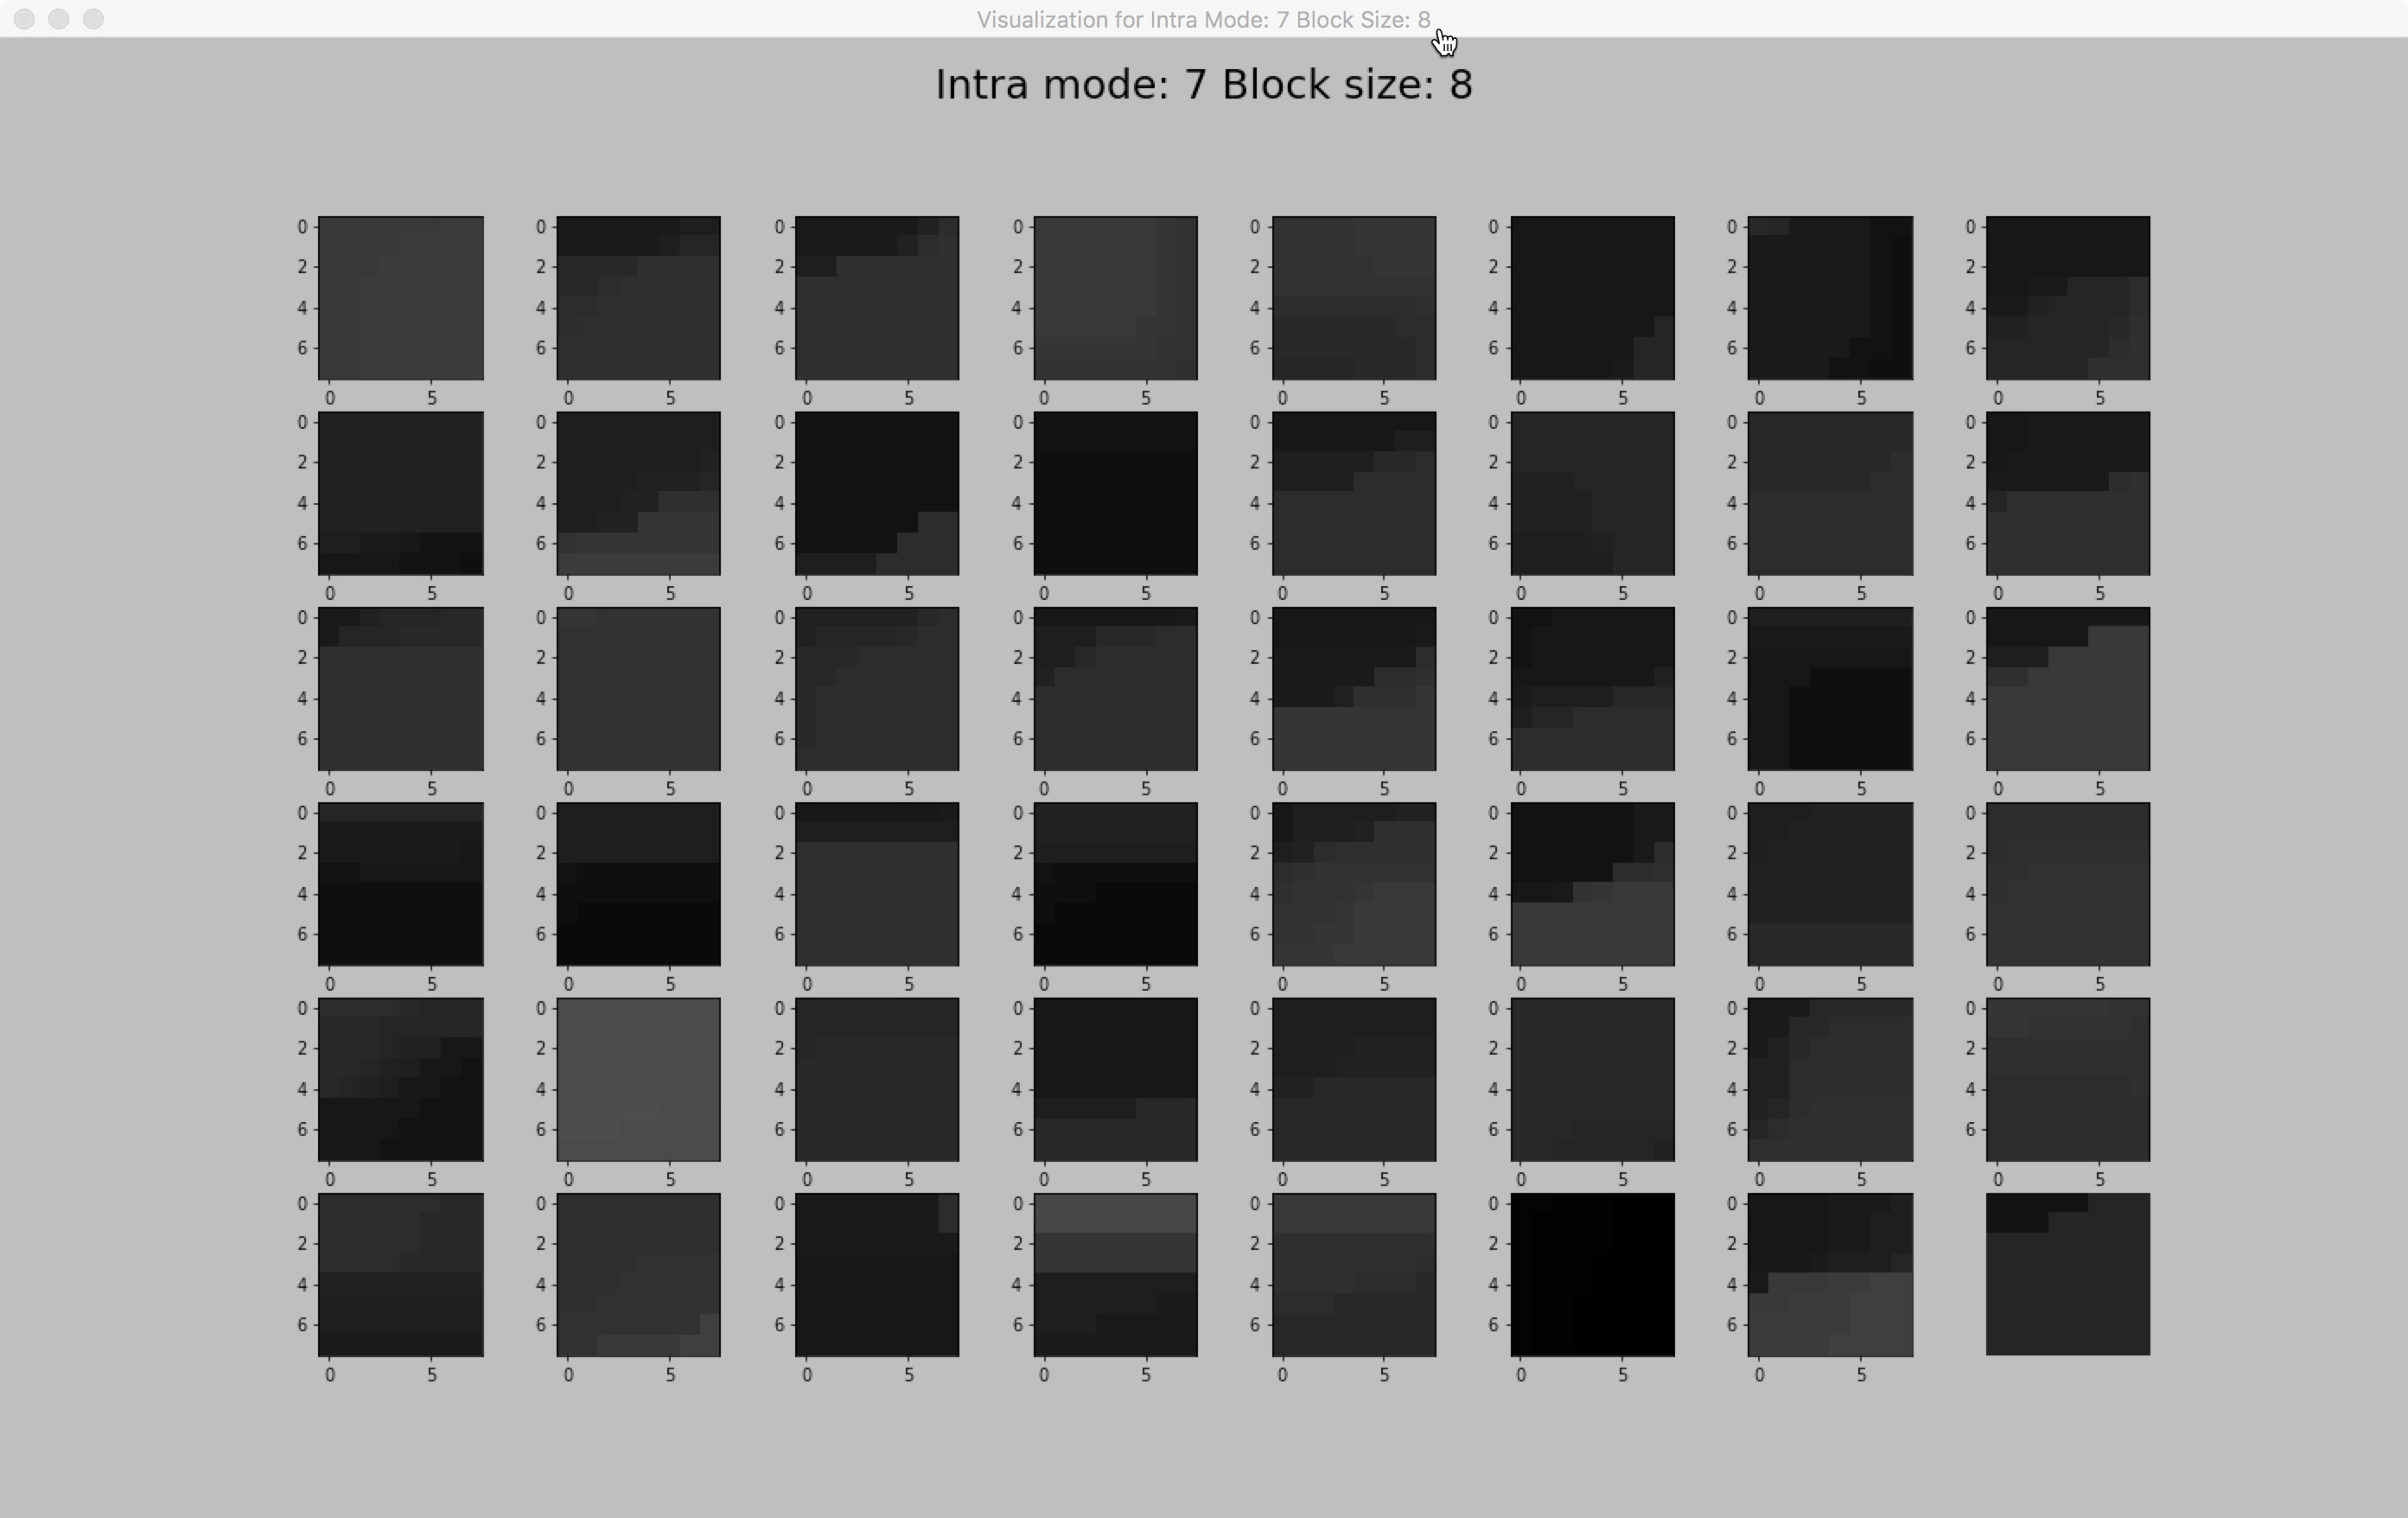
\includegraphics[width=\linewidth]{Figures/visu-size8x8/8-7}
            \caption[Visualizations for blocks tagged with intra mode 7]{Visualizations for blocks tagged with intra mode 7.}
            \label{fig:size8_mode7}
        \end{minipage}
        
        \vspace*{1cm} % vertical separation
    
        \begin{minipage}{0.49\textwidth}
            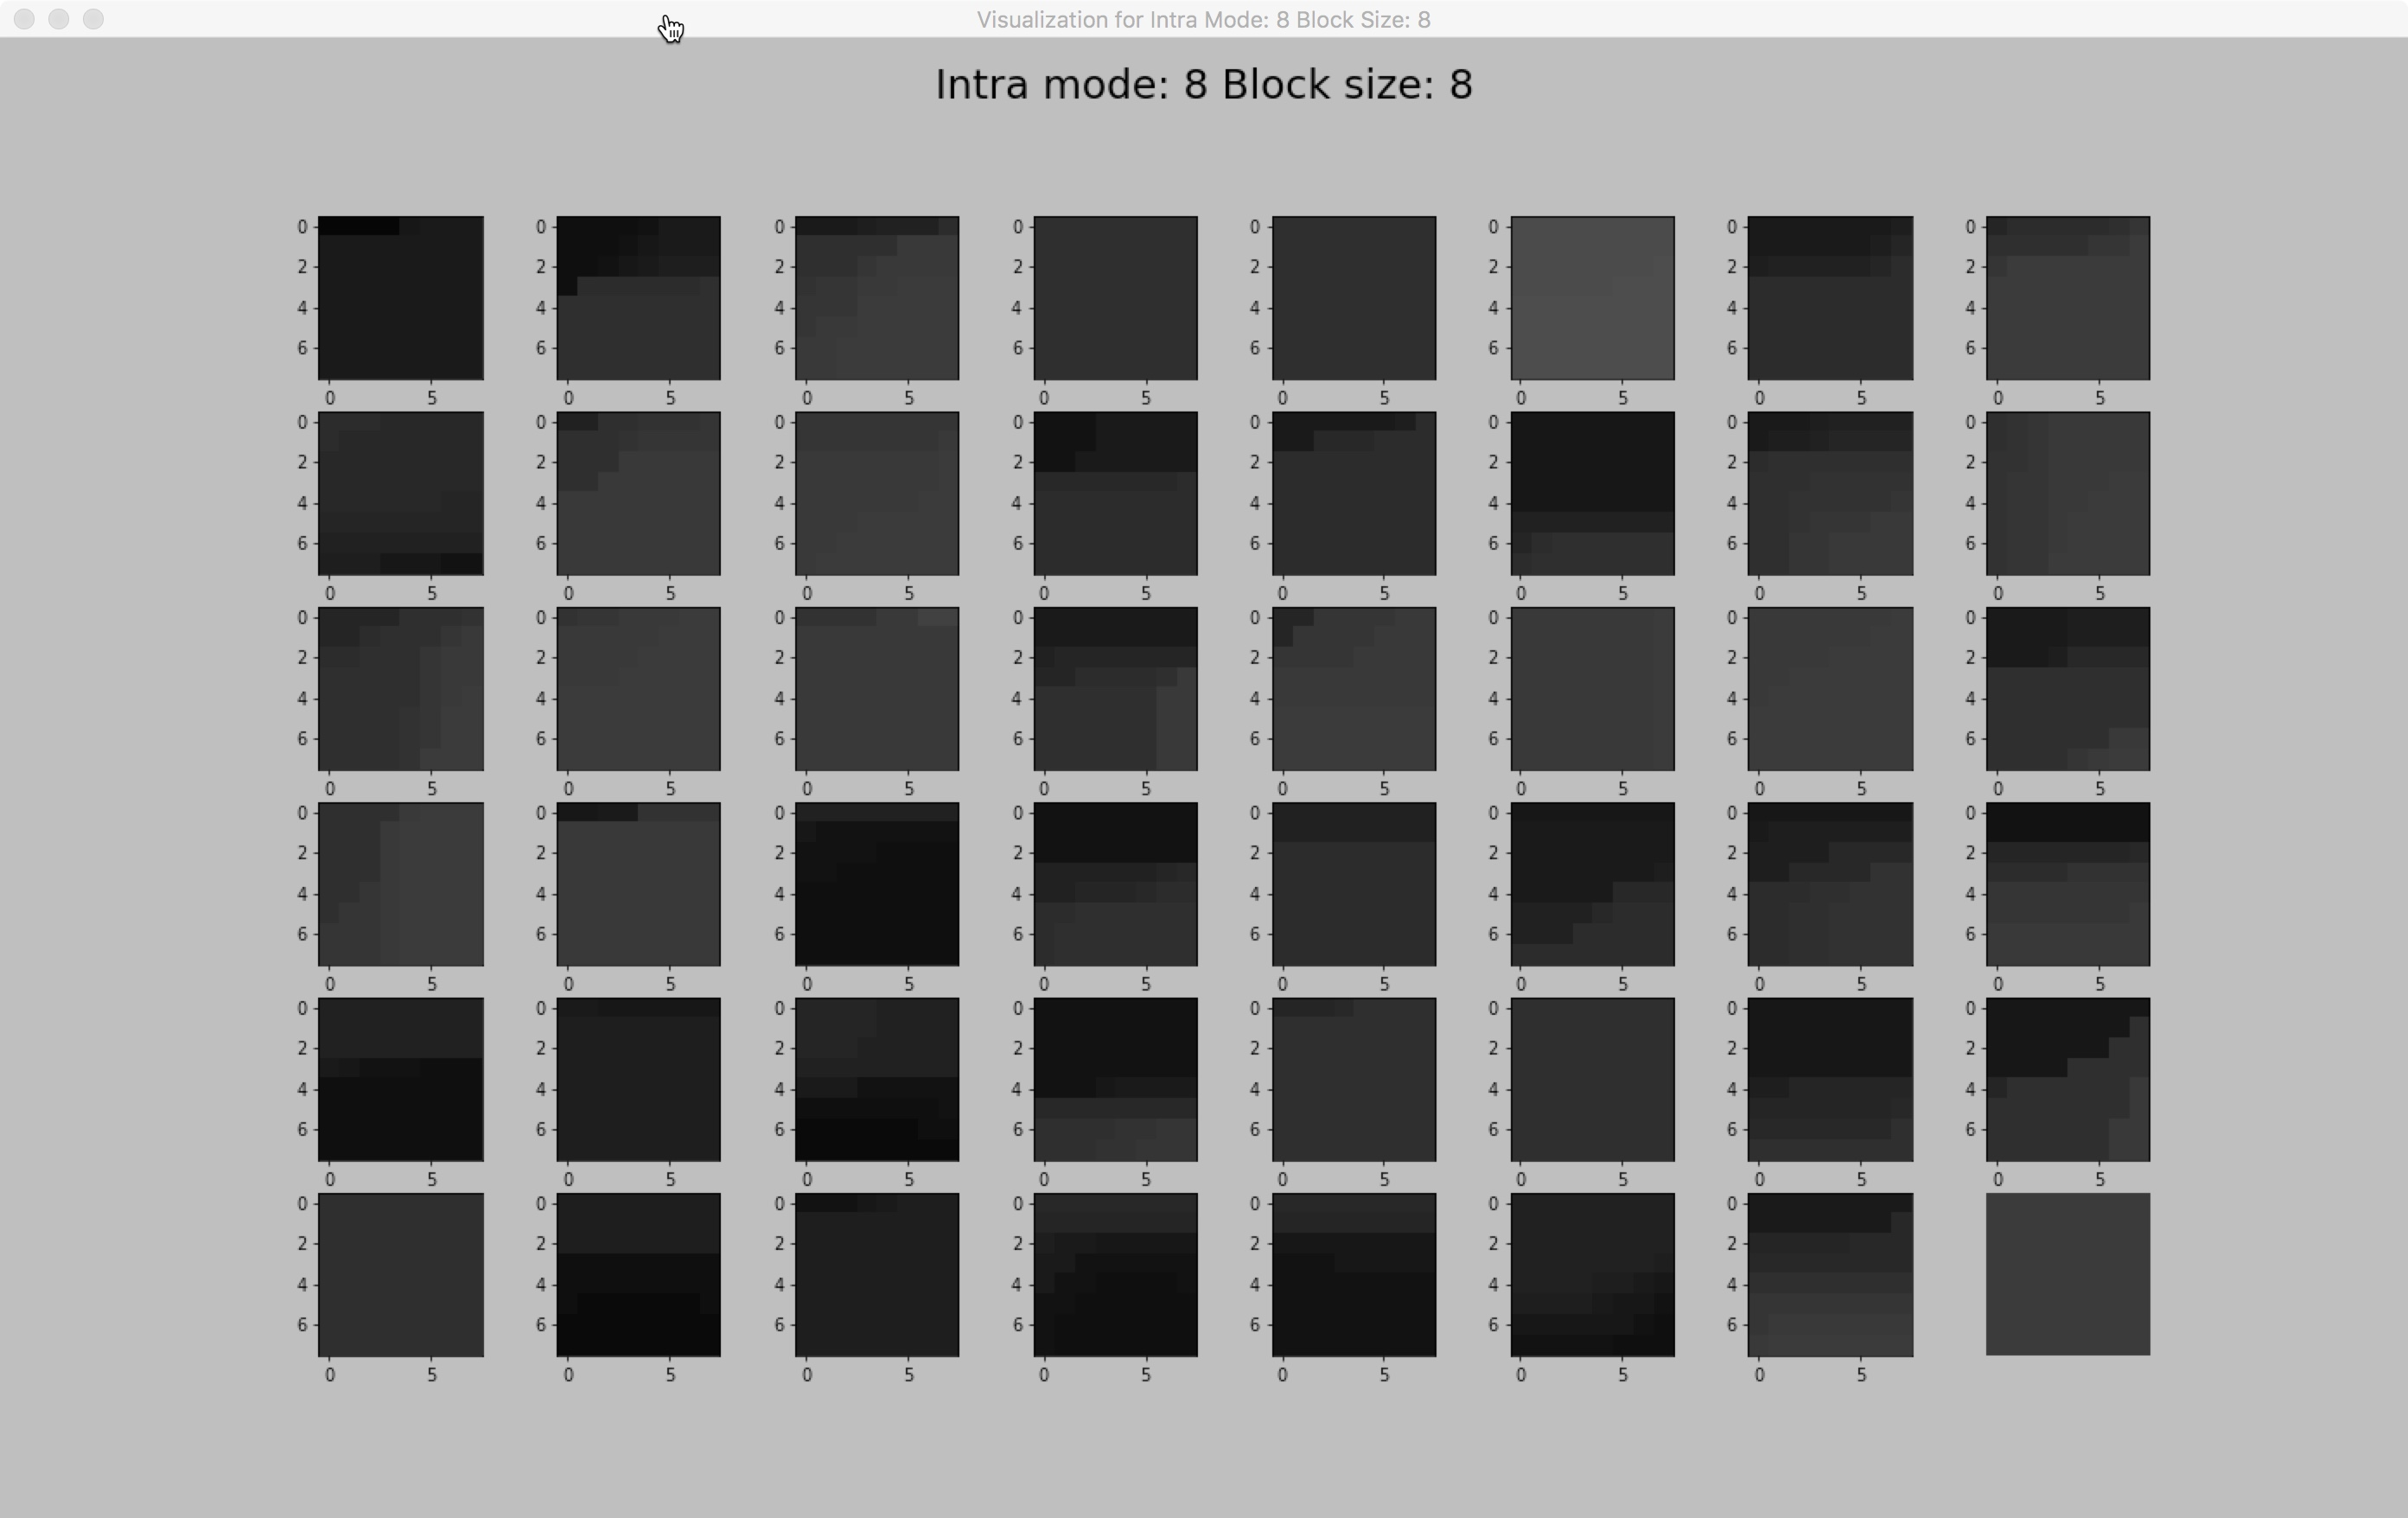
\includegraphics[width=\linewidth]{Figures/visu-size8x8/8-8}
            \caption[Visualizations for blocks tagged with intra mode 8]{Visualizations for blocks tagged with intra mode 8.}
            \label{fig:size8_mode8}
        \end{minipage}
        \hspace{\fill} % note: no blank line here
        \begin{minipage}{0.49\textwidth}
            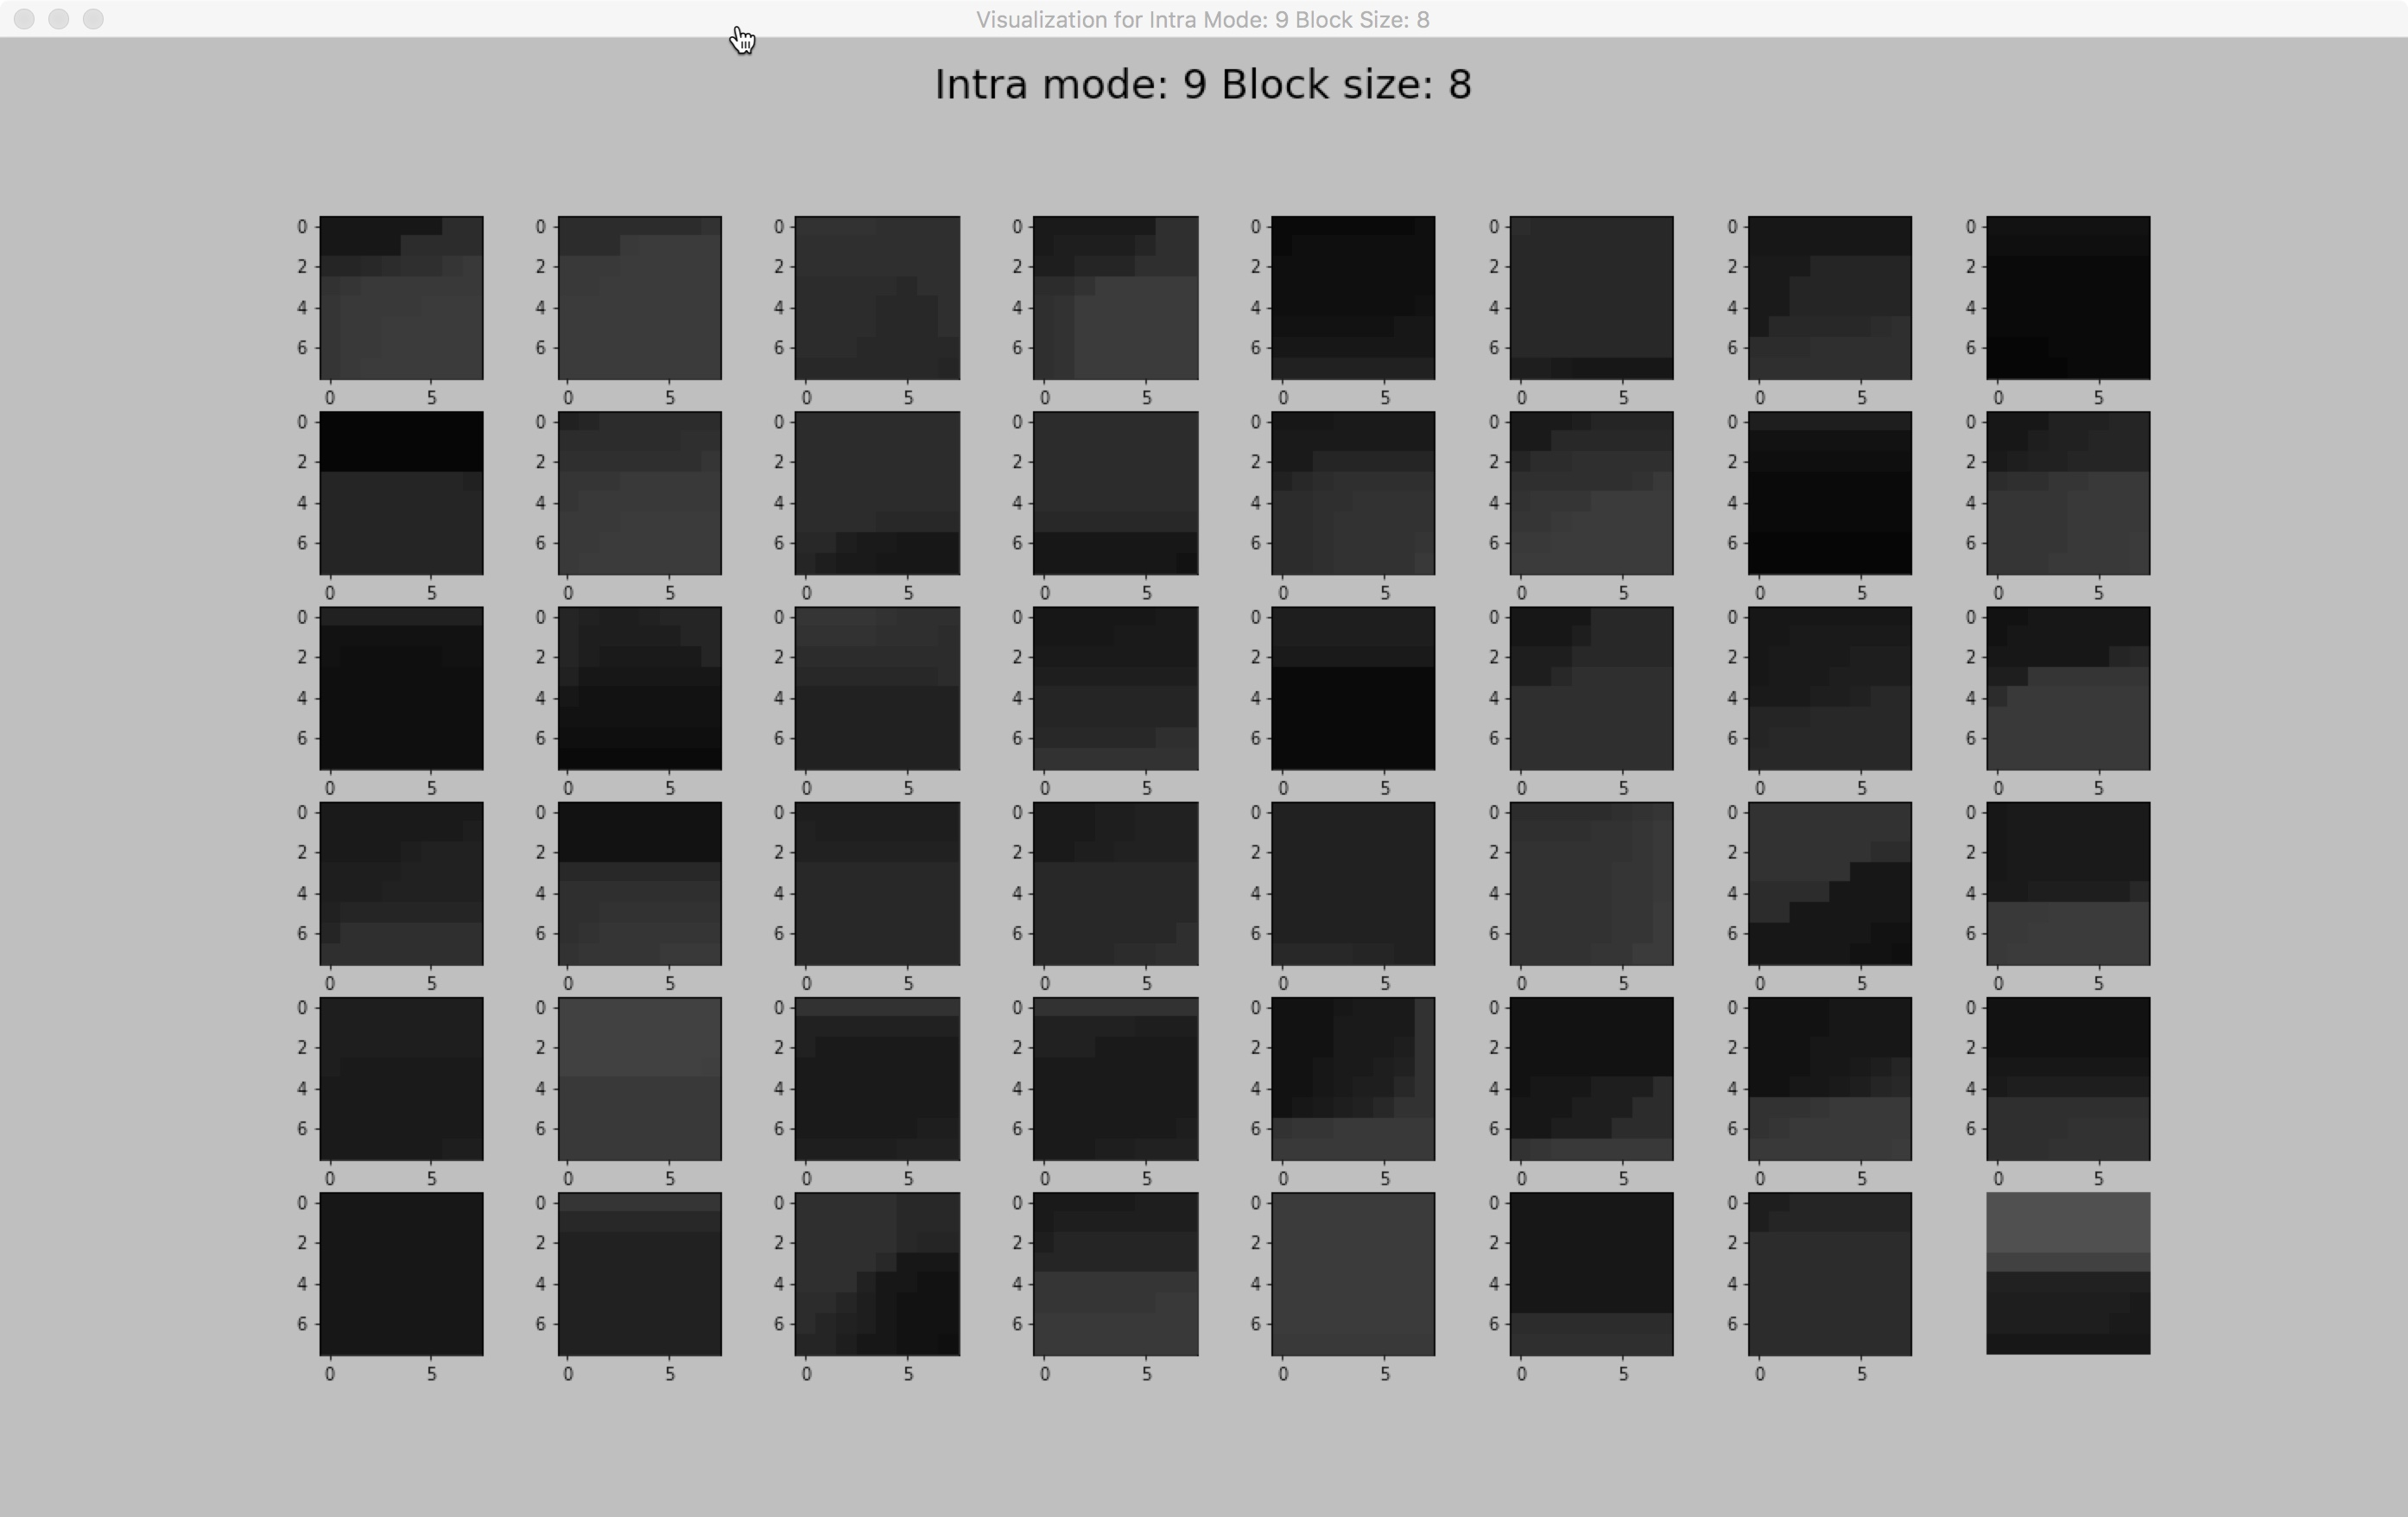
\includegraphics[width=\linewidth]{Figures/visu-size8x8/8-9}
            \caption[Visualizations for blocks tagged with intra mode 9]{Visualizations for blocks tagged with intra mode 9.}
            \label{fig:size8_mode9}
        \end{minipage}
    % \caption{Figure caption goes here}\label{fig:see-data-visu}
    \end{figure}
    
    \begin{figure}
    
        \vspace*{1cm} % vertical separation
    
        \begin{minipage}{0.49\textwidth}
            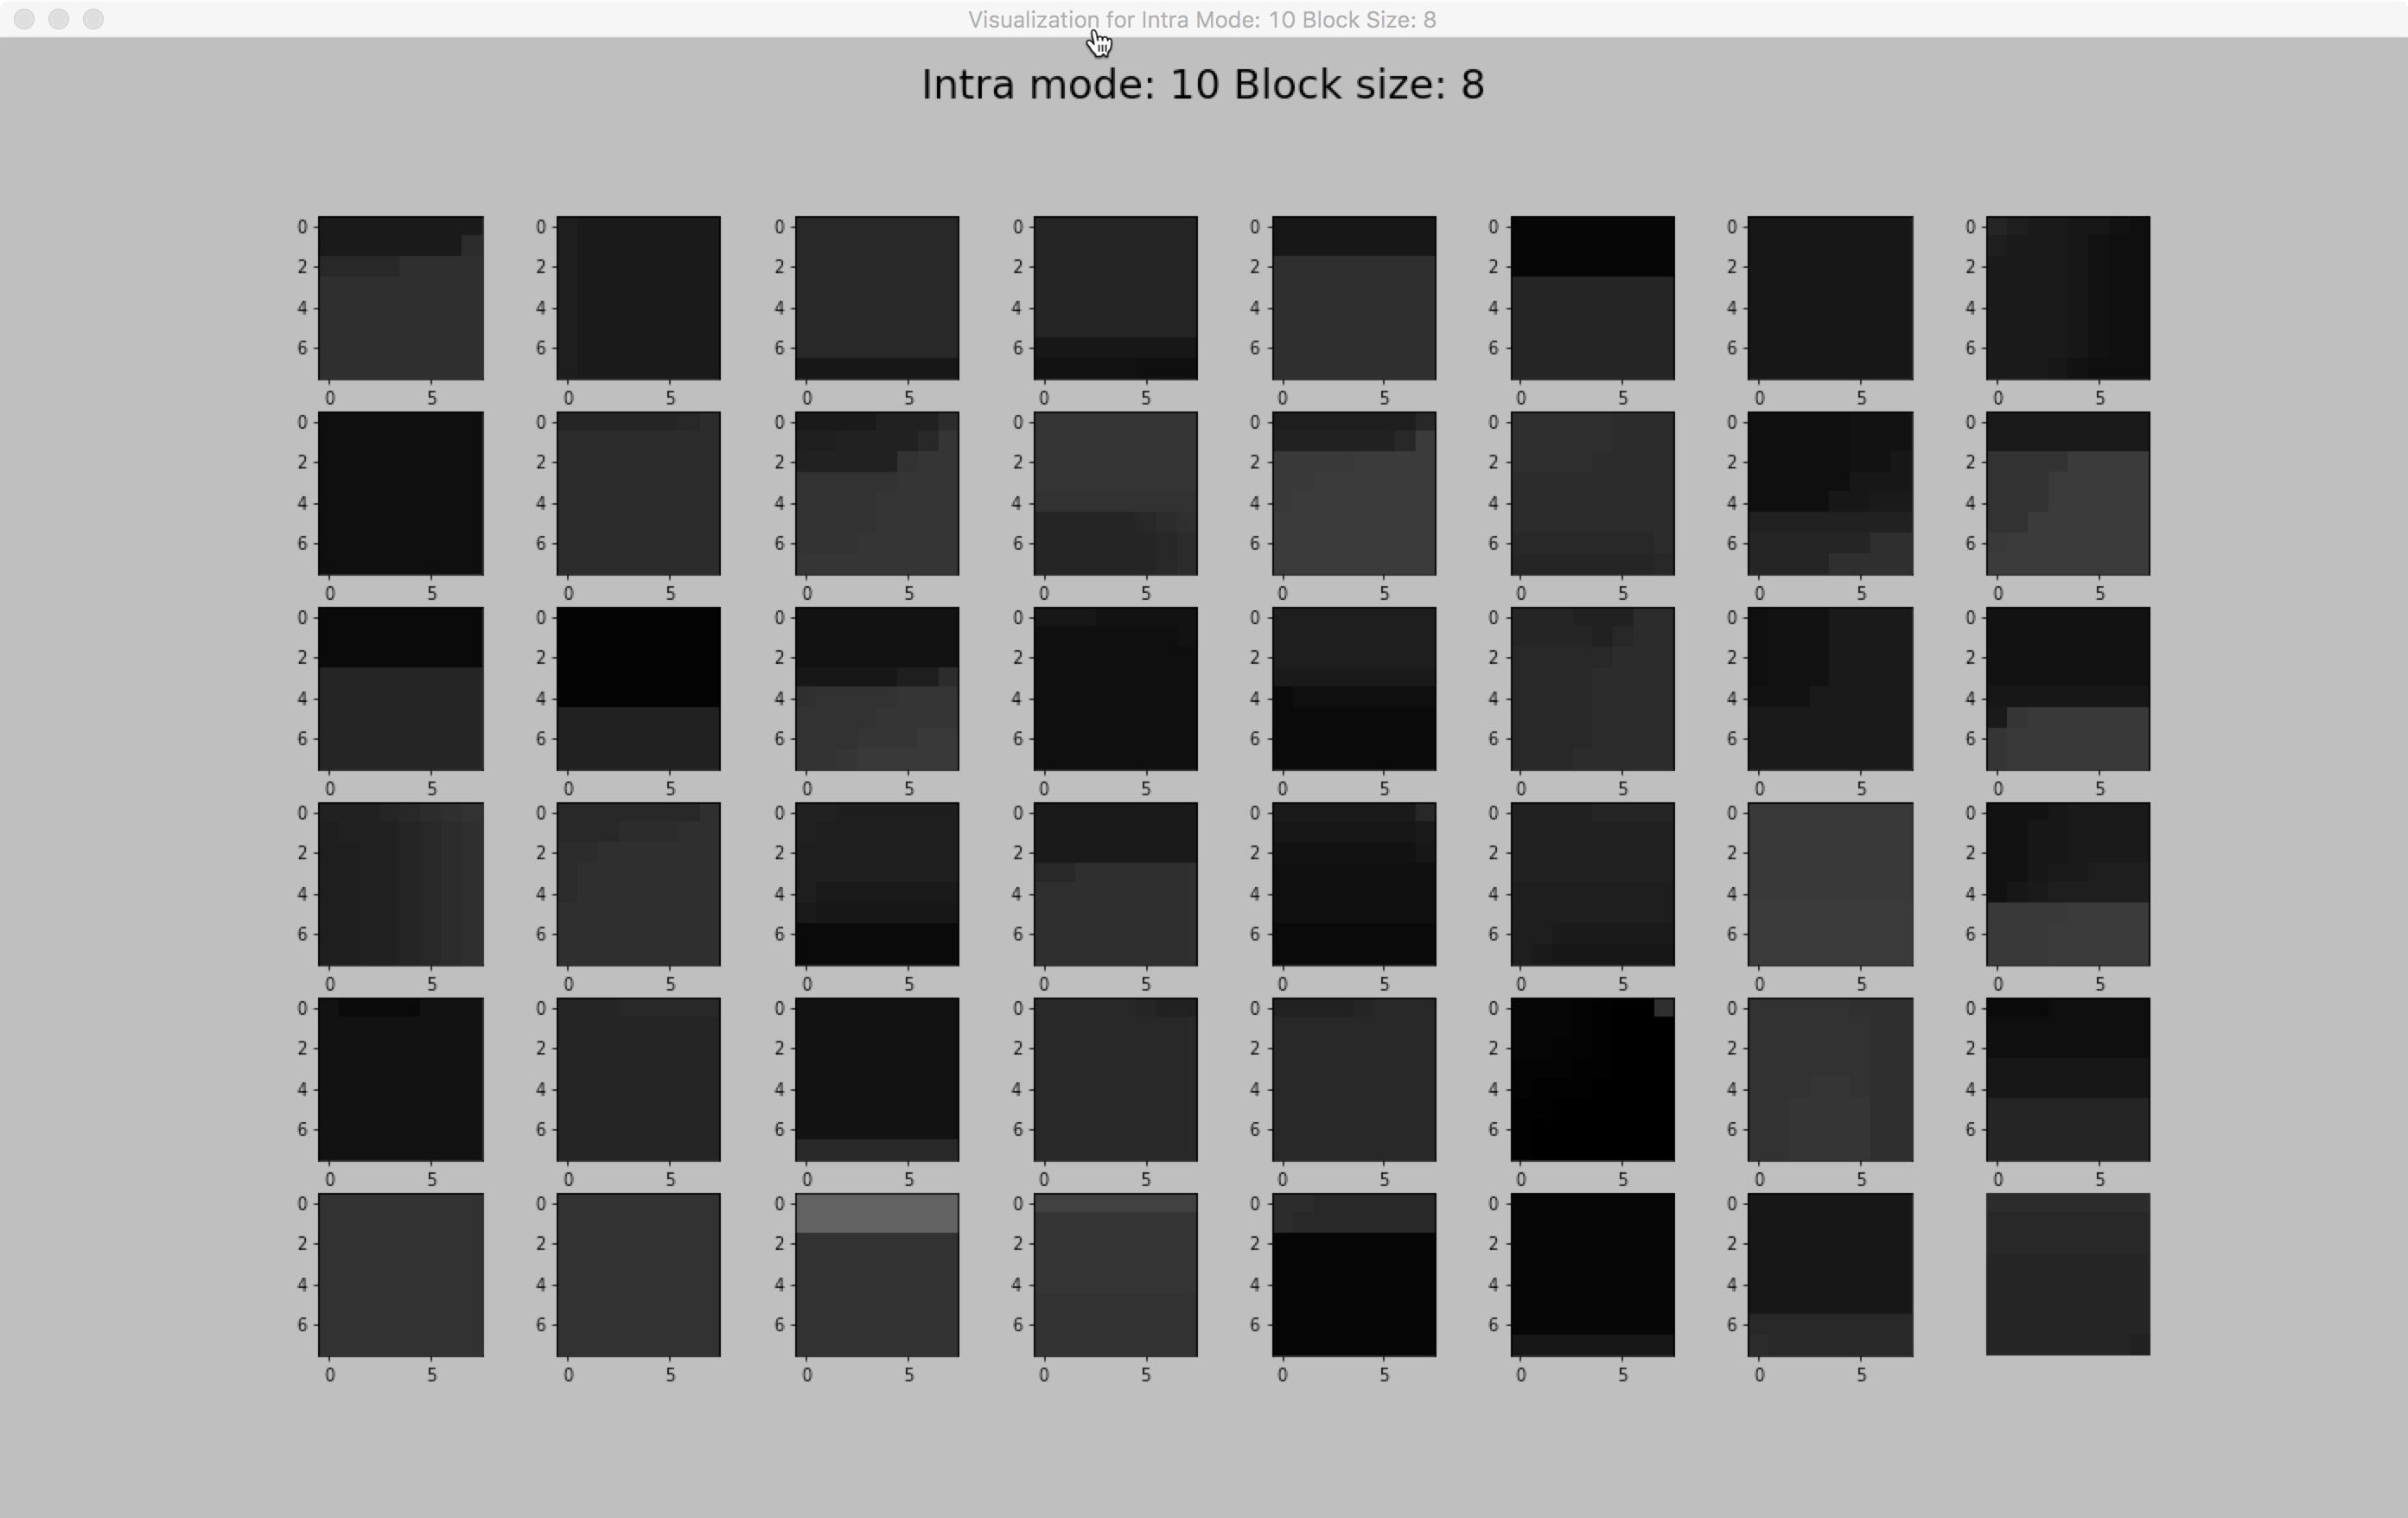
\includegraphics[width=\linewidth]{Figures/visu-size8x8/8-10}
            \caption[Visualizations for blocks tagged with intra mode 10]{Visualizations for blocks tagged with intra mode 10.}
            \label{fig:size8_mode4}
        \end{minipage}
        \hspace{\fill} % note: no blank line here
        \begin{minipage}{0.49\textwidth}
            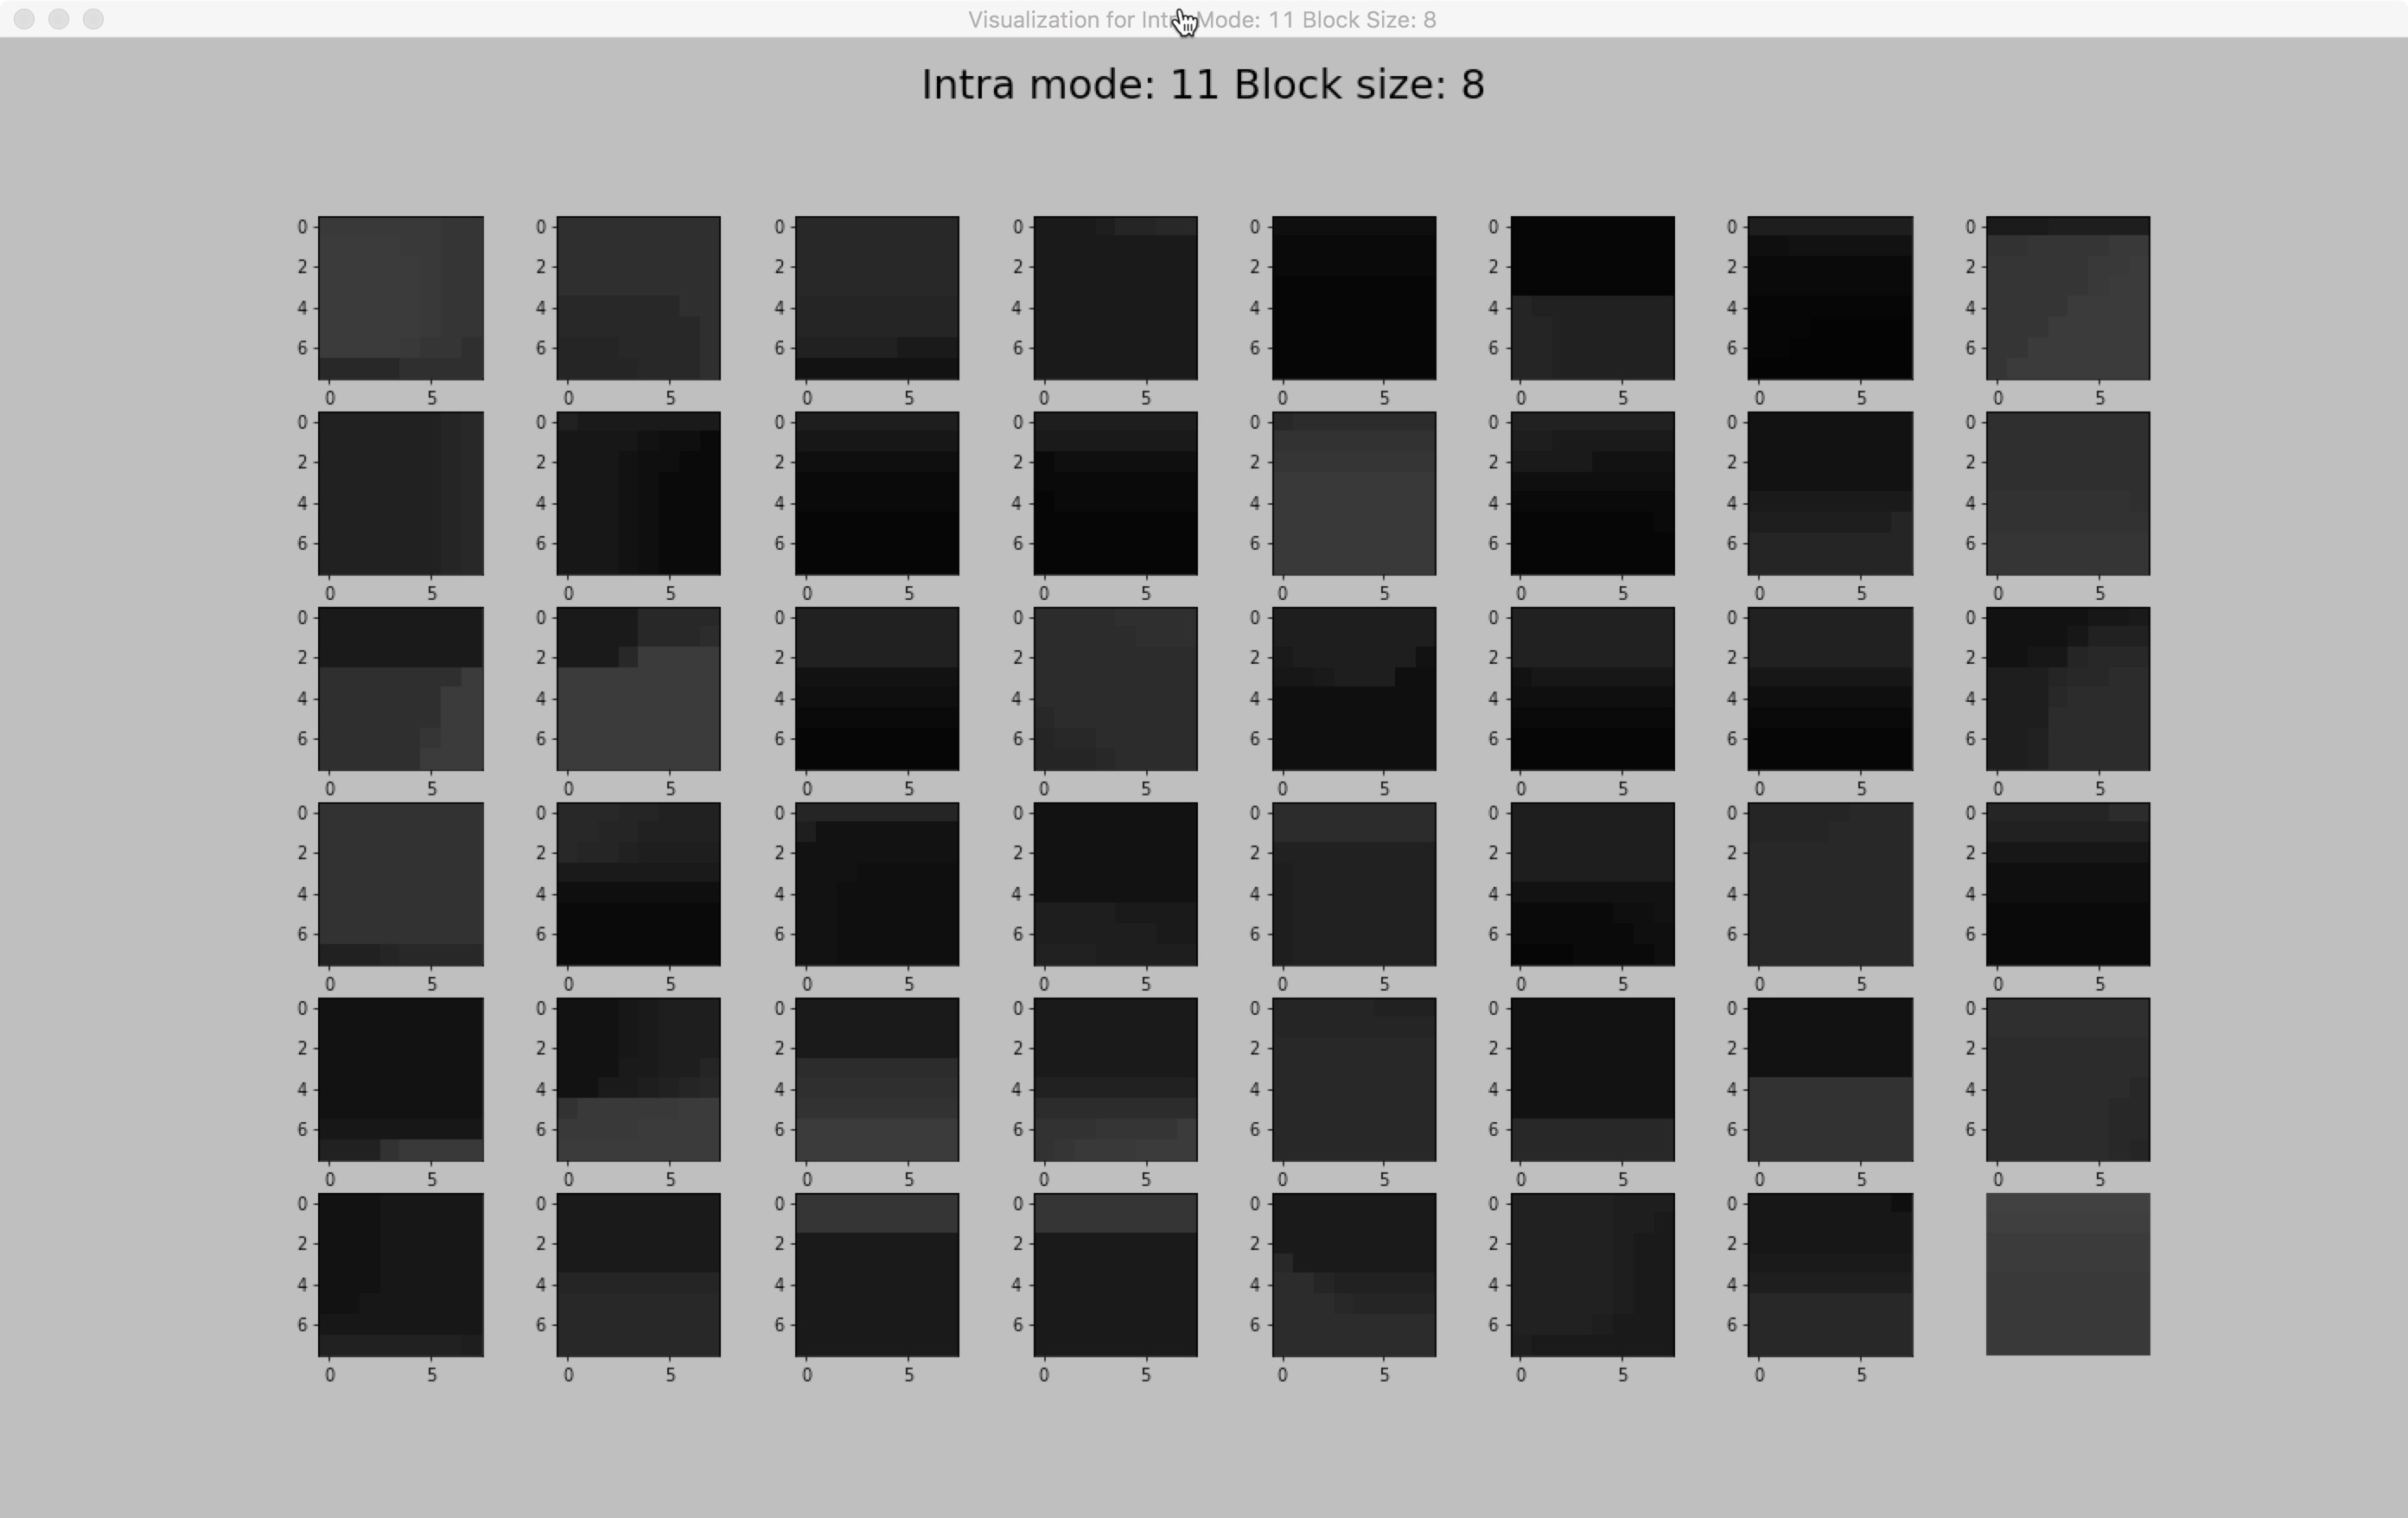
\includegraphics[width=\linewidth]{Figures/visu-size8x8/8-11}
            \caption[Visualizations for blocks tagged with intra mode 11]{Visualizations for blocks tagged with intra mode 11.}
            \label{fig:size8_mode11}
        \end{minipage}
        
        \vspace*{1cm} % vertical separation
        
        \begin{minipage}{0.49\textwidth}
            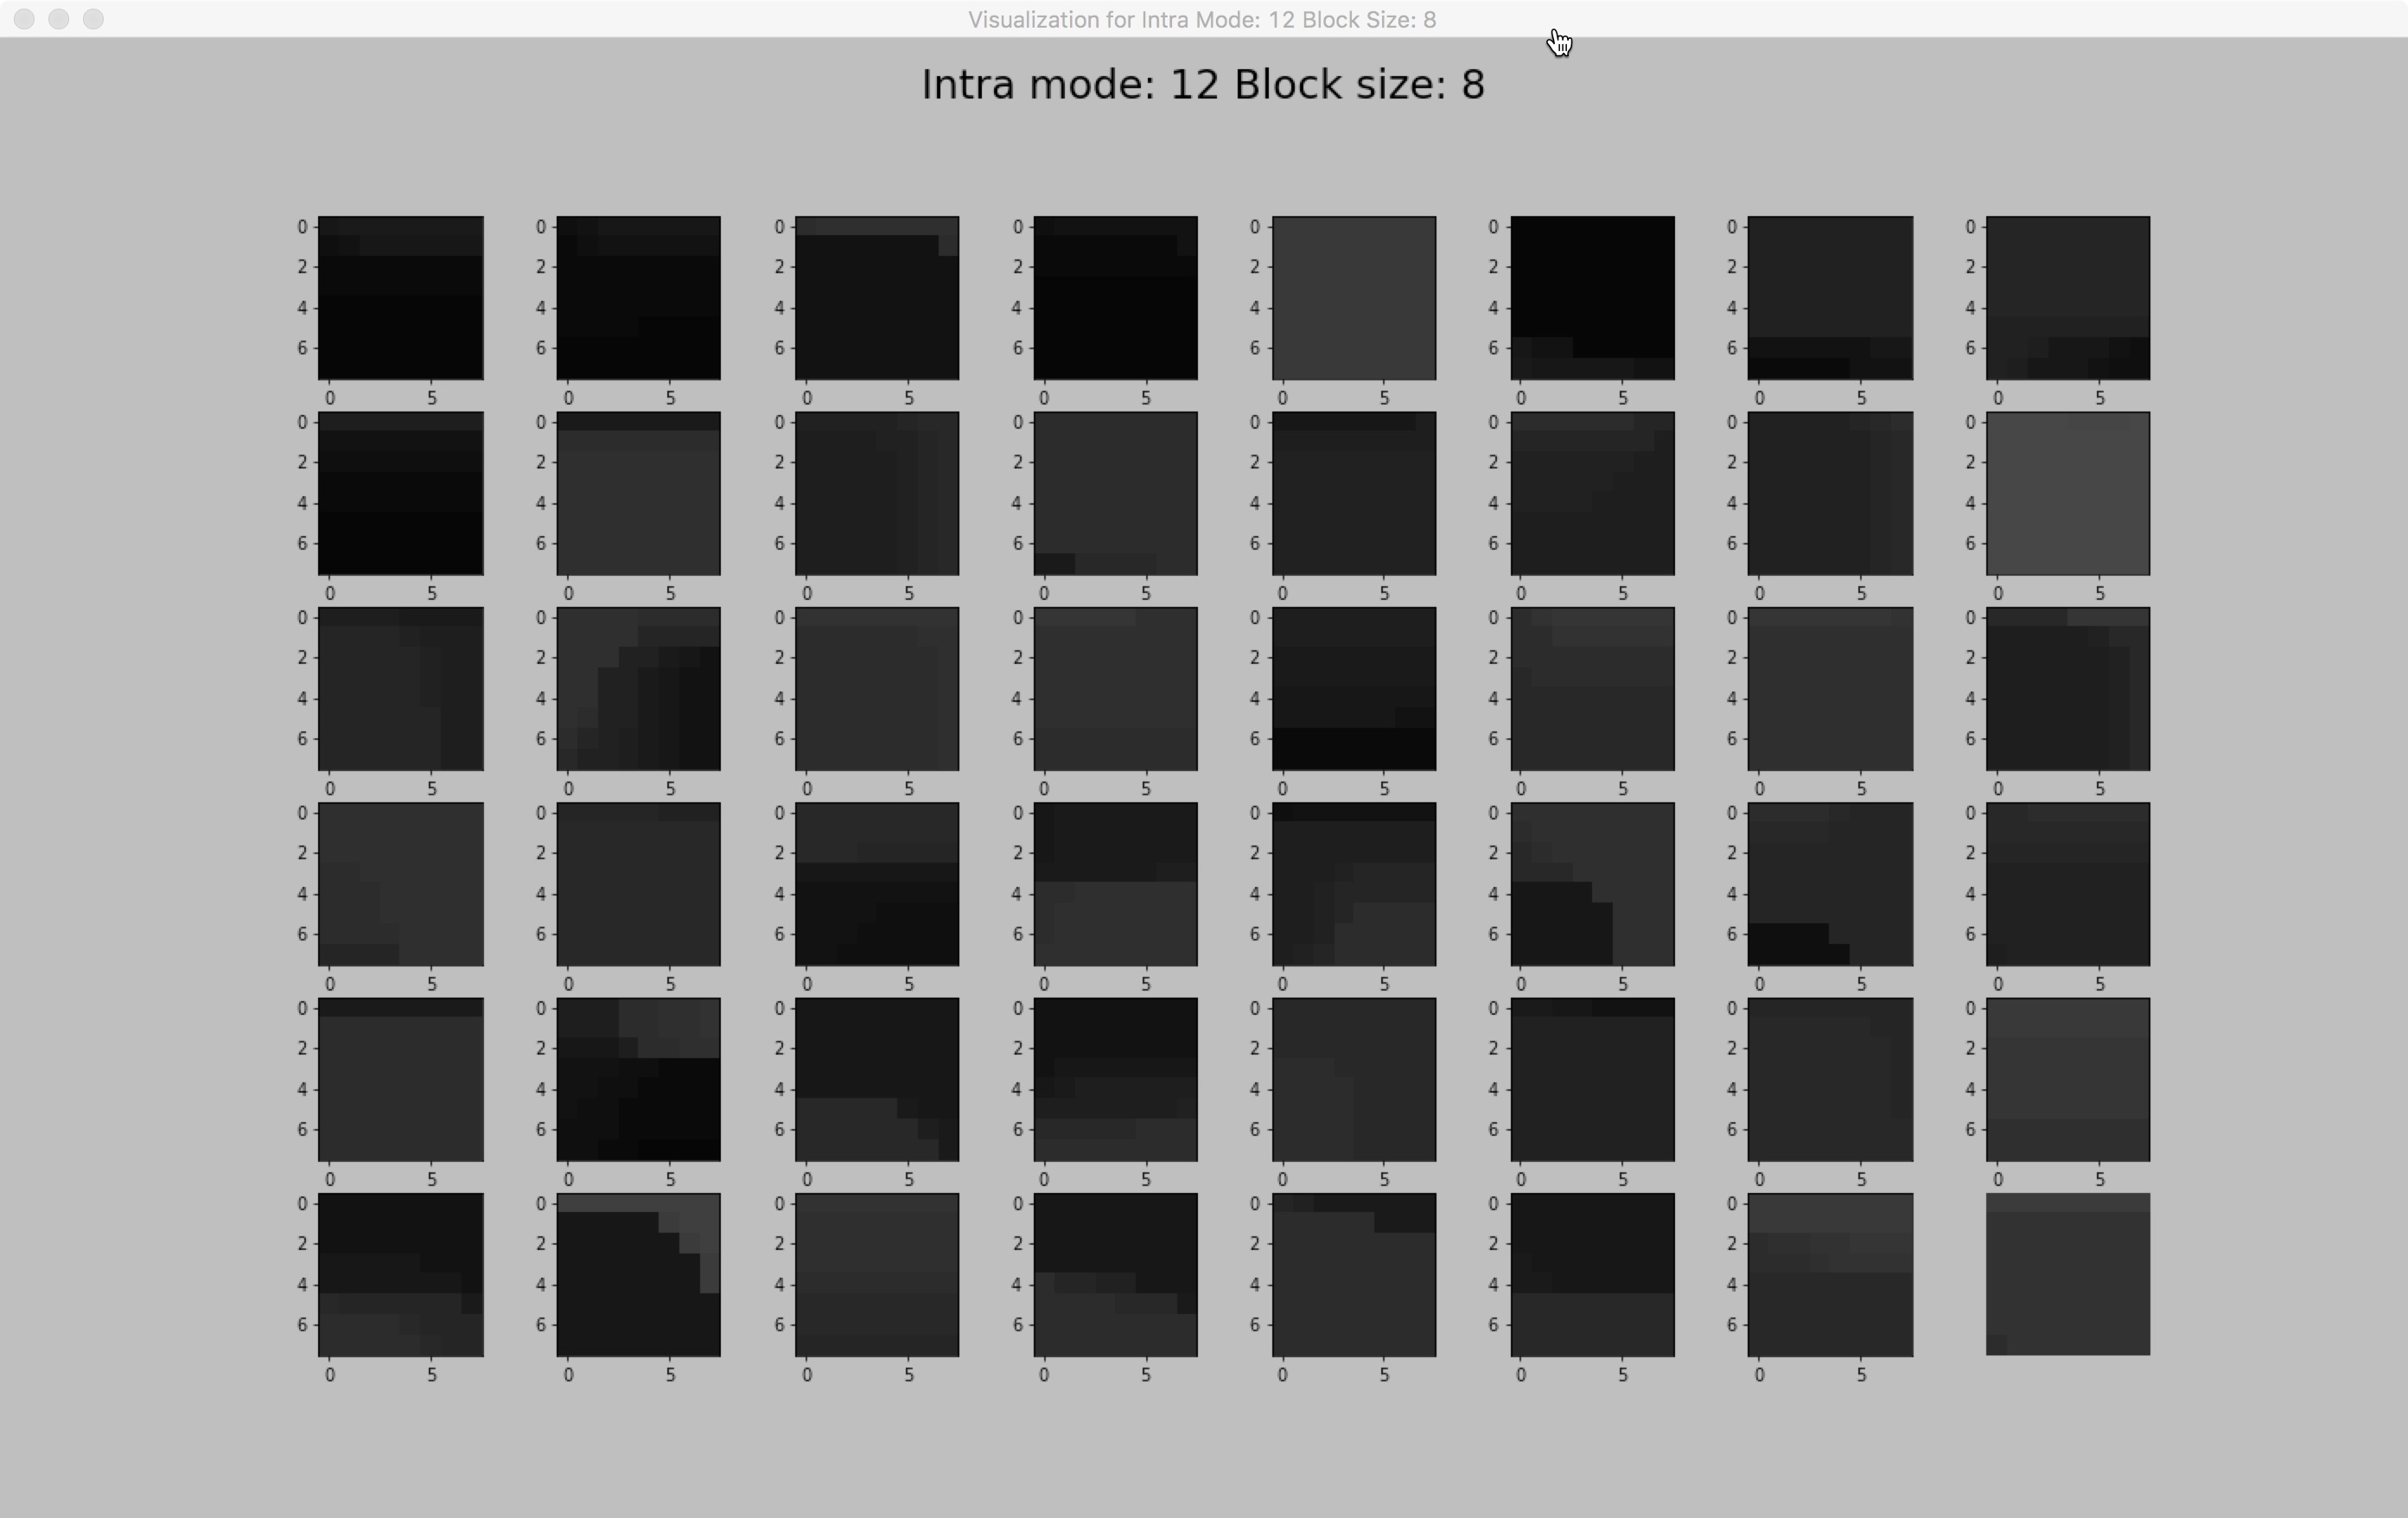
\includegraphics[width=\linewidth]{Figures/visu-size8x8/8-12}
            \caption[Visualizations for blocks tagged with intra mode 12]{Visualizations for blocks tagged with intra mode 12.}
            \label{fig:size8_mode12}
        \end{minipage}
        \hspace{\fill} % note: no blank line here
        \begin{minipage}{0.49\textwidth}
            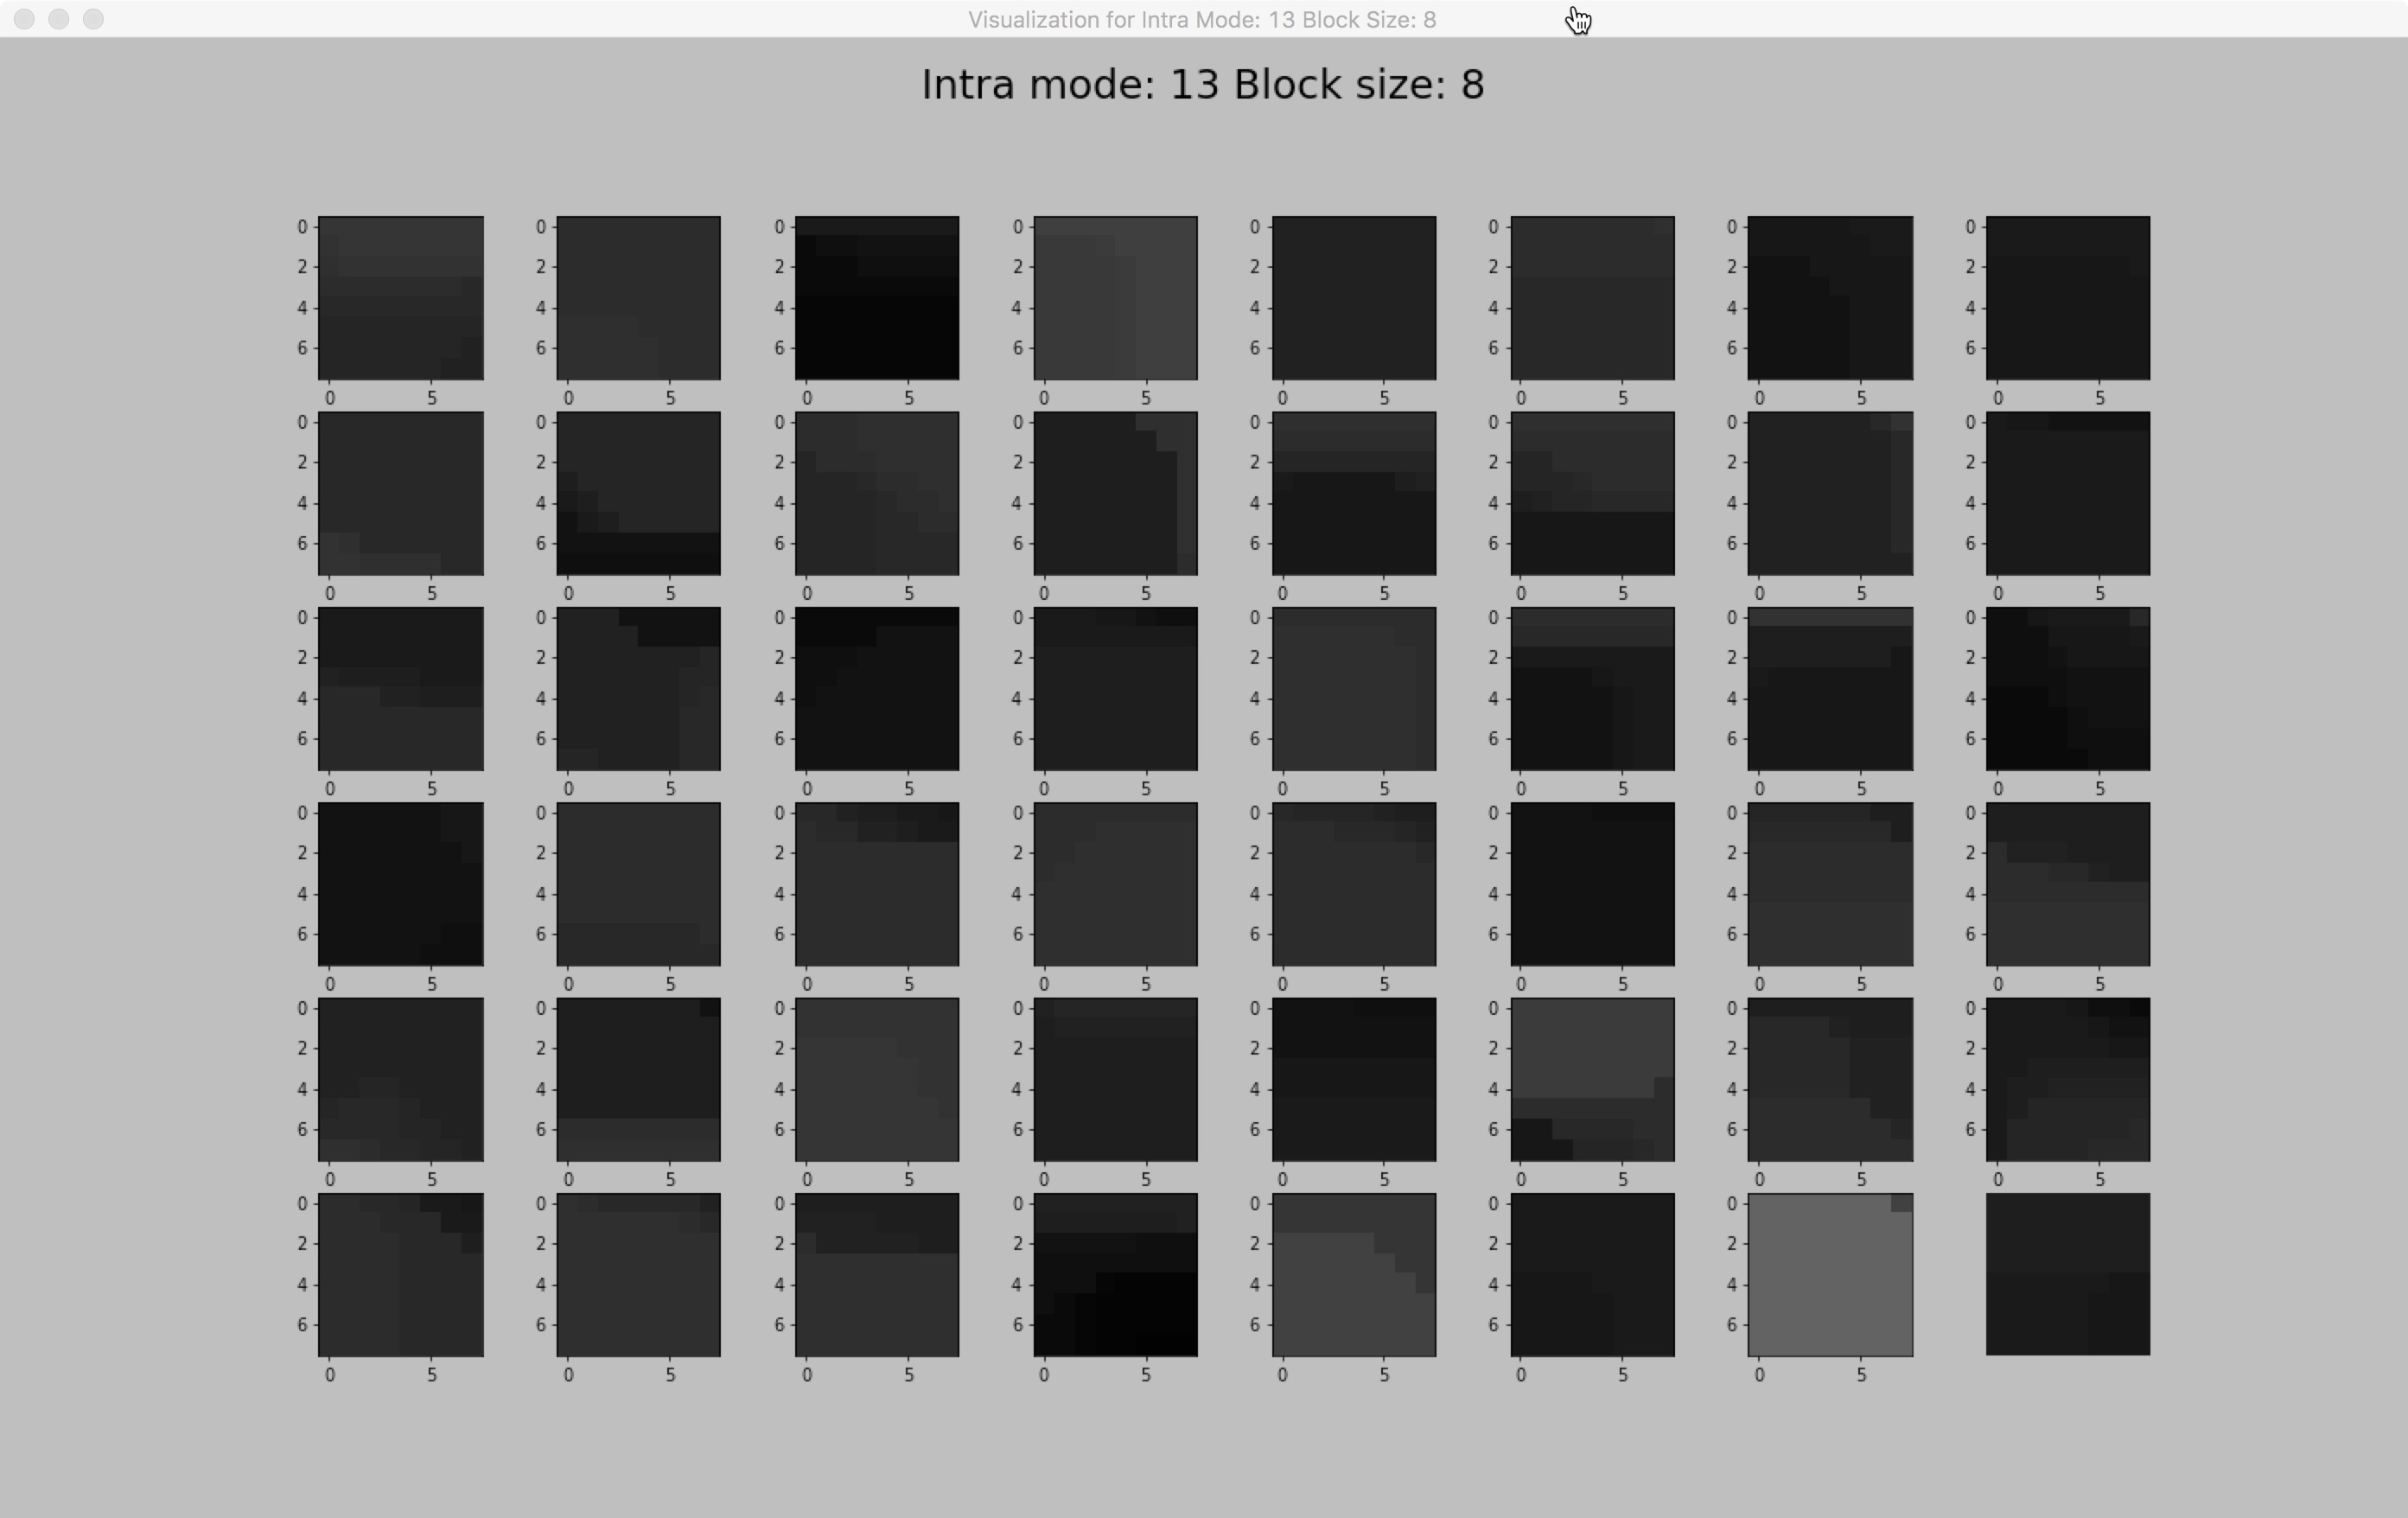
\includegraphics[width=\linewidth]{Figures/visu-size8x8/8-13}
            \caption[Visualizations for blocks tagged with intra mode 13]{Visualizations for blocks tagged with intra mode 13.}
            \label{fig:size8_mode13}
        \end{minipage}
        
        \vspace*{1cm} % vertical separation
    
        \begin{minipage}{0.49\textwidth}
            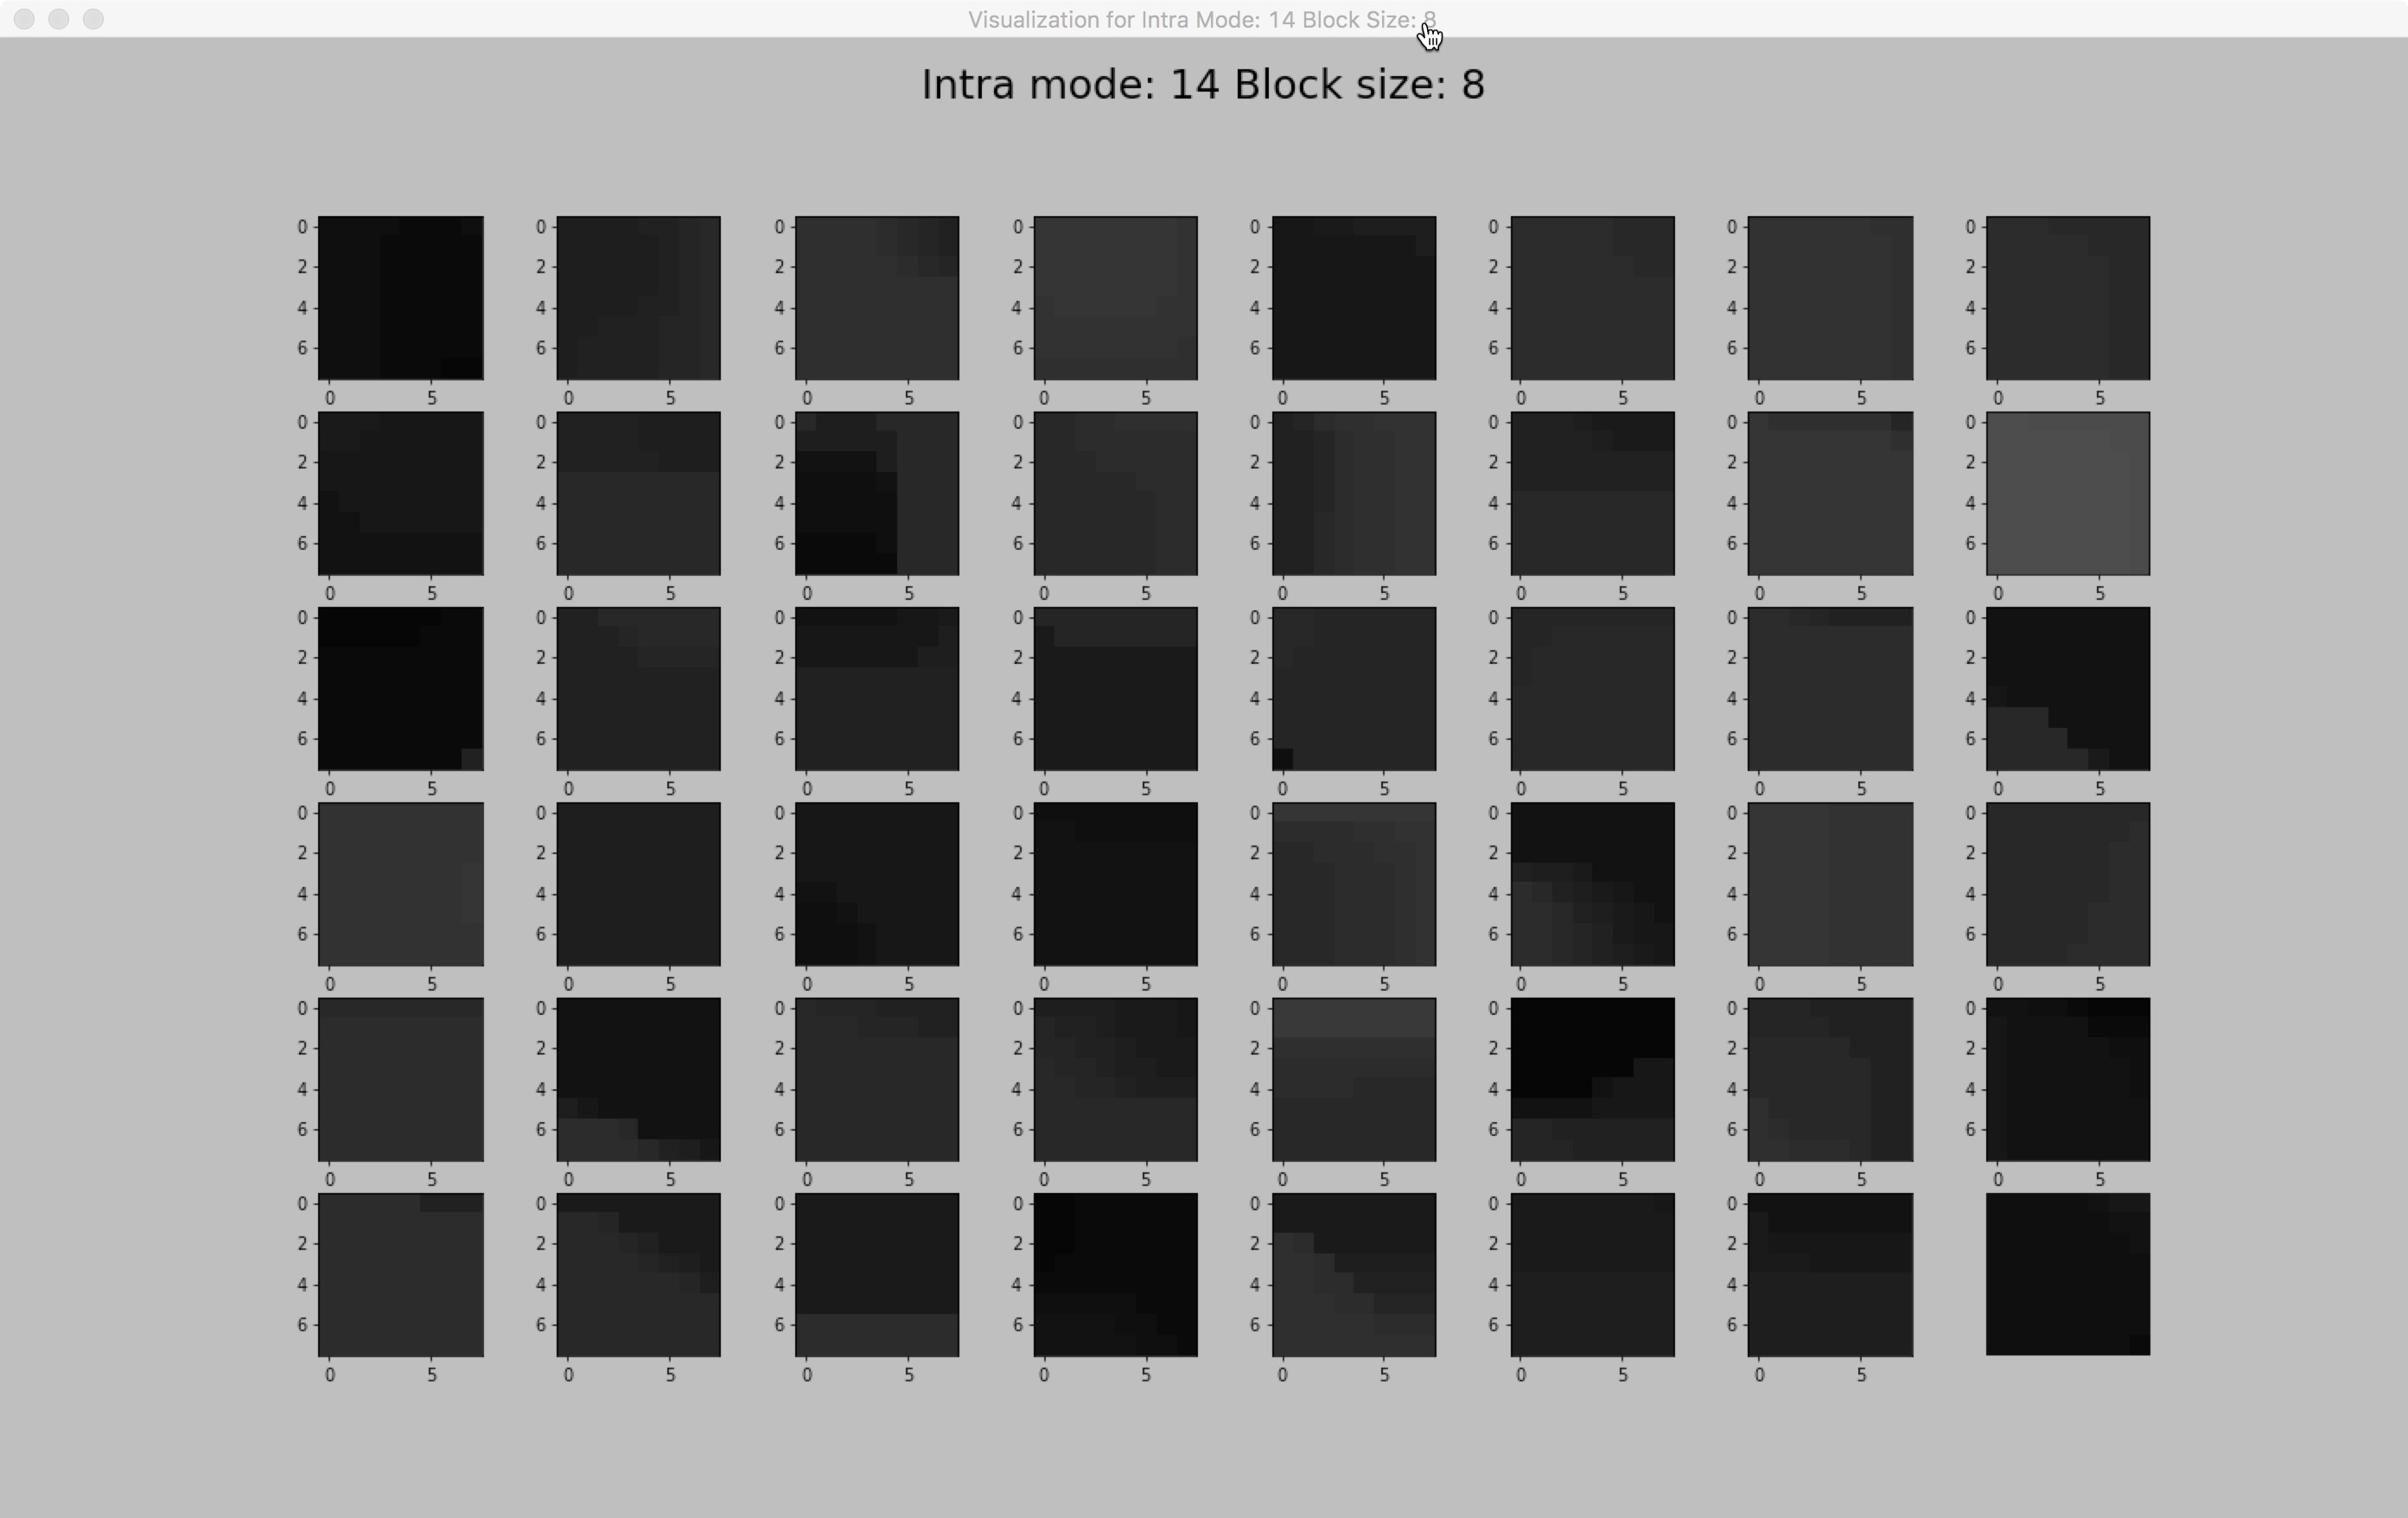
\includegraphics[width=\linewidth]{Figures/visu-size8x8/8-14}
            \caption[Visualizations for blocks tagged with intra mode 14]{Visualizations for blocks tagged with intra mode 14.}
            \label{fig:size8_mode14}
        \end{minipage}
        \hspace{\fill} % note: no blank line here
        \begin{minipage}{0.49\textwidth}
            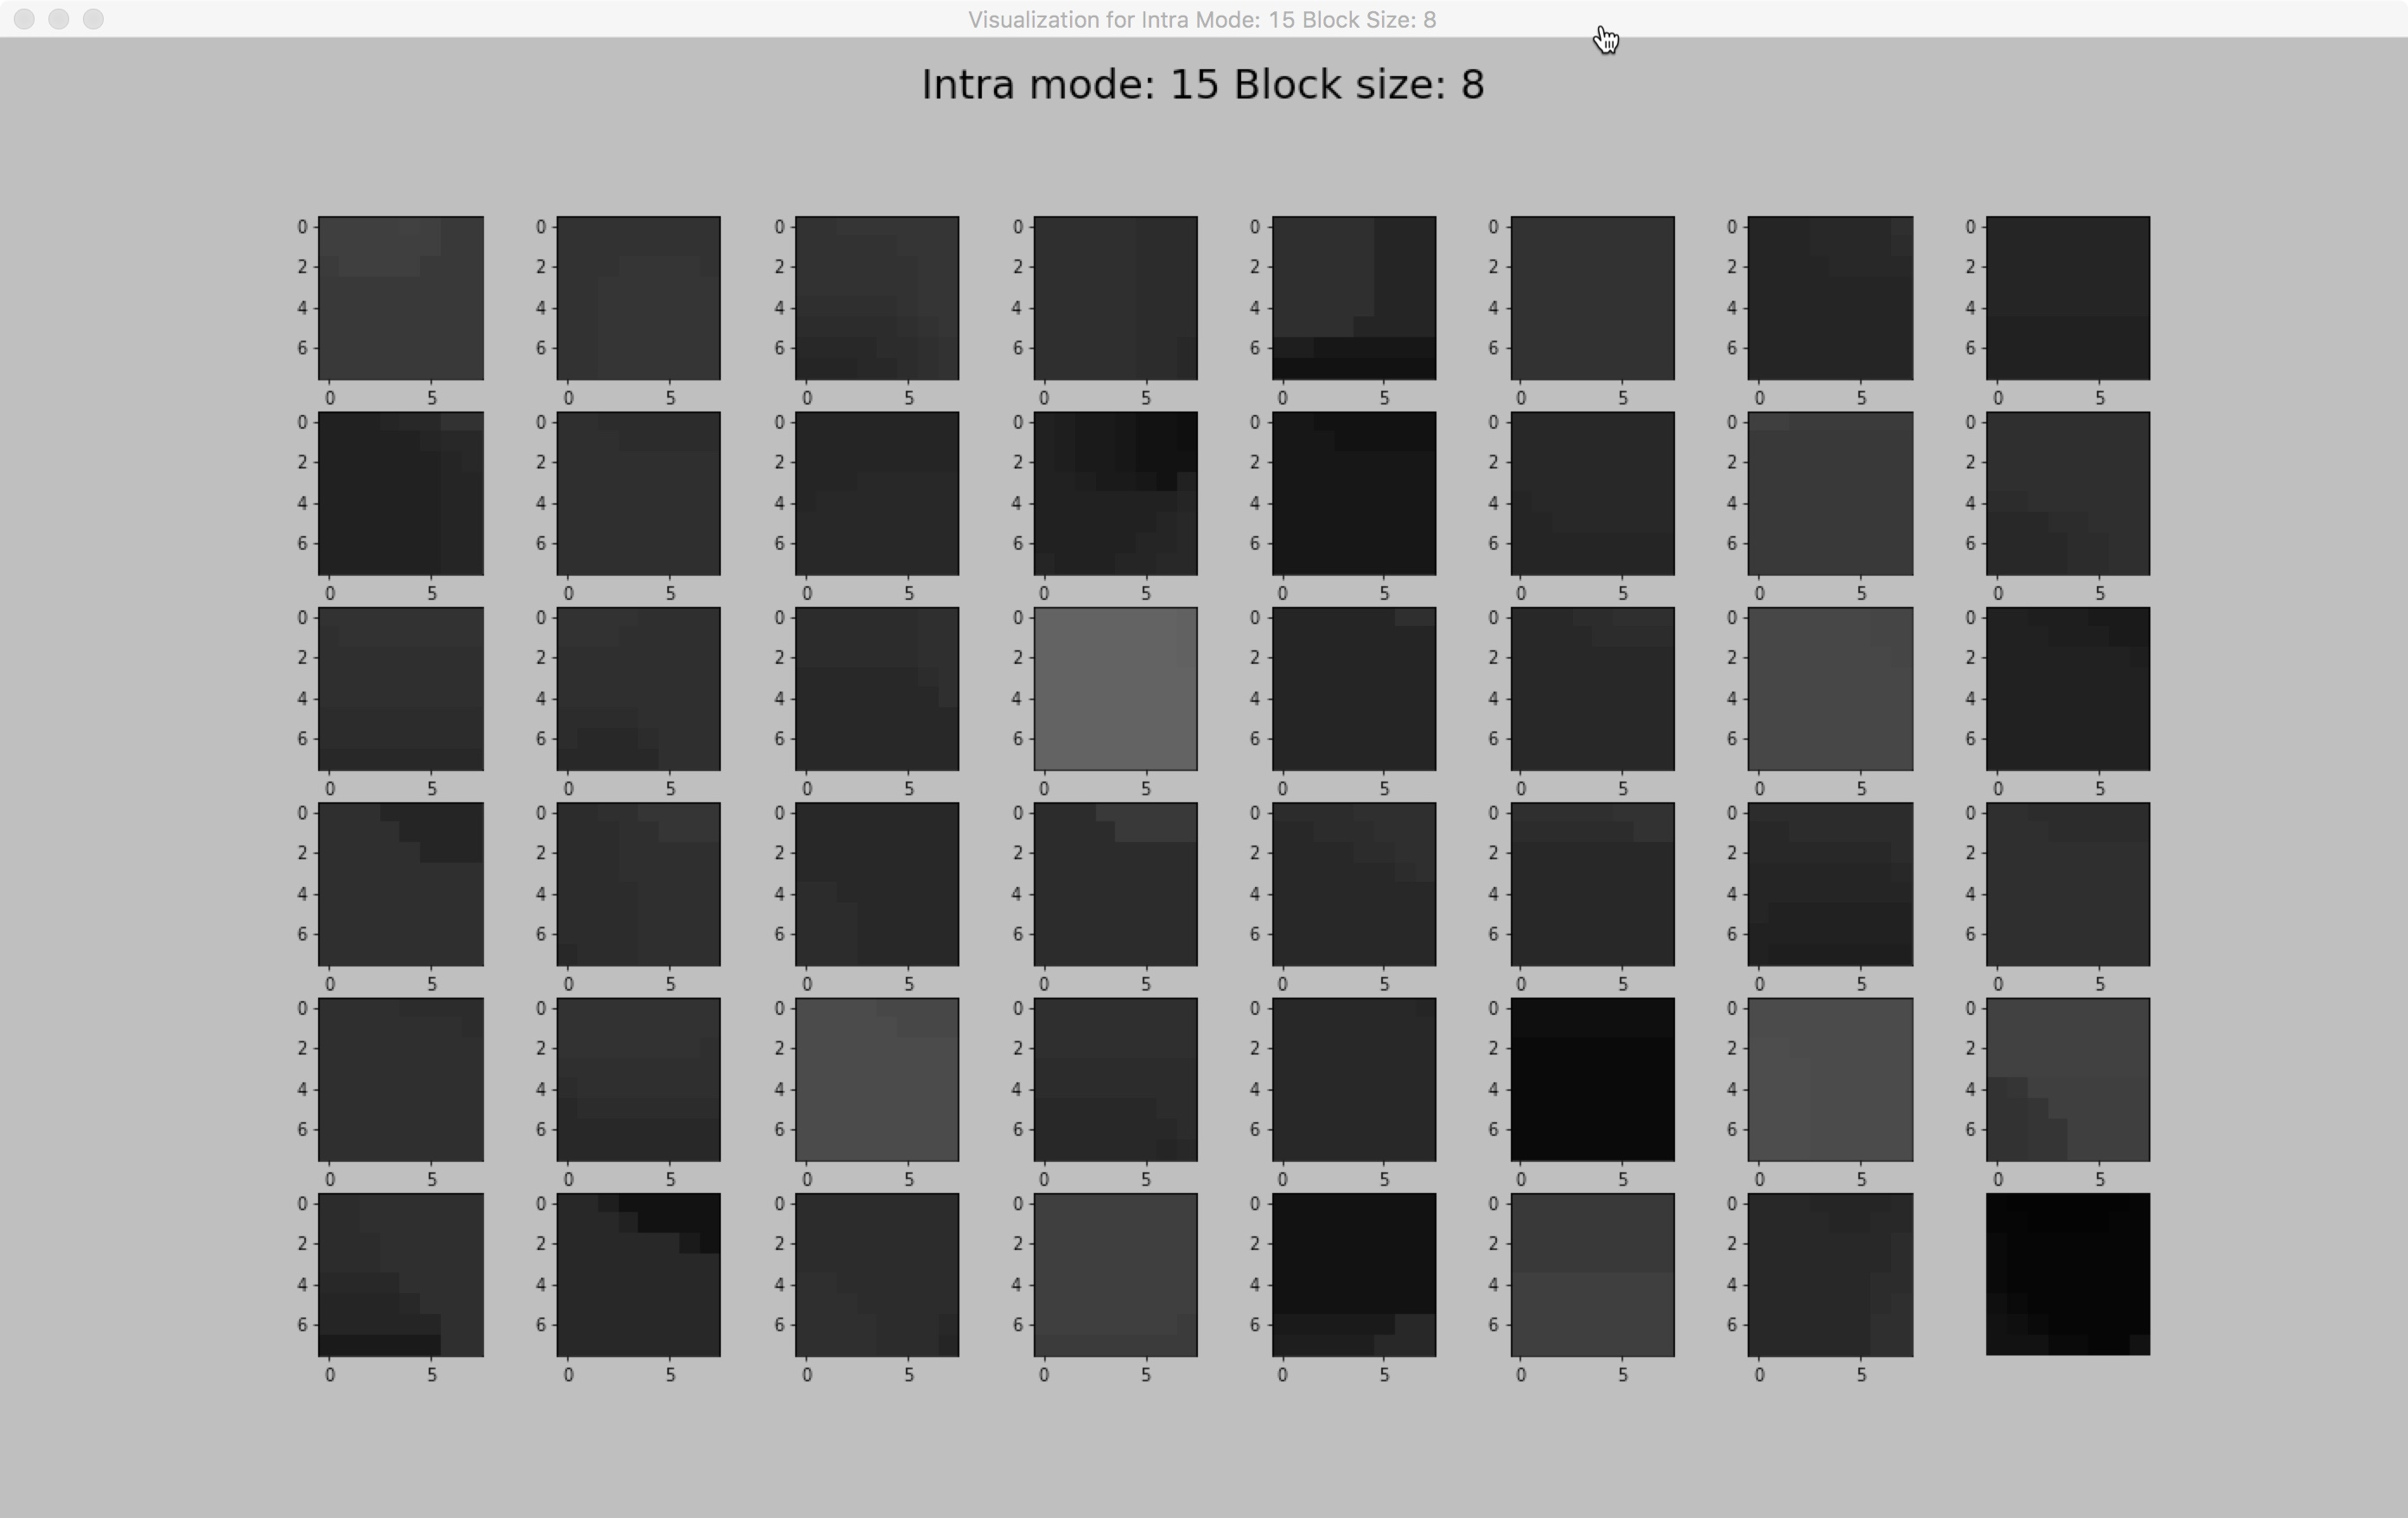
\includegraphics[width=\linewidth]{Figures/visu-size8x8/8-15}
            \caption[Visualizations for blocks tagged with intra mode 15]{Visualizations for blocks tagged with intra mode 15.}
            \label{fig:size8_mode15}
        \end{minipage}
    % \caption{Figure caption goes here}\label{fig:see-data-visu}
    \end{figure}
    
    \begin{figure}
    
        \vspace*{1cm} % vertical separation
    
        \begin{minipage}{0.49\textwidth}
            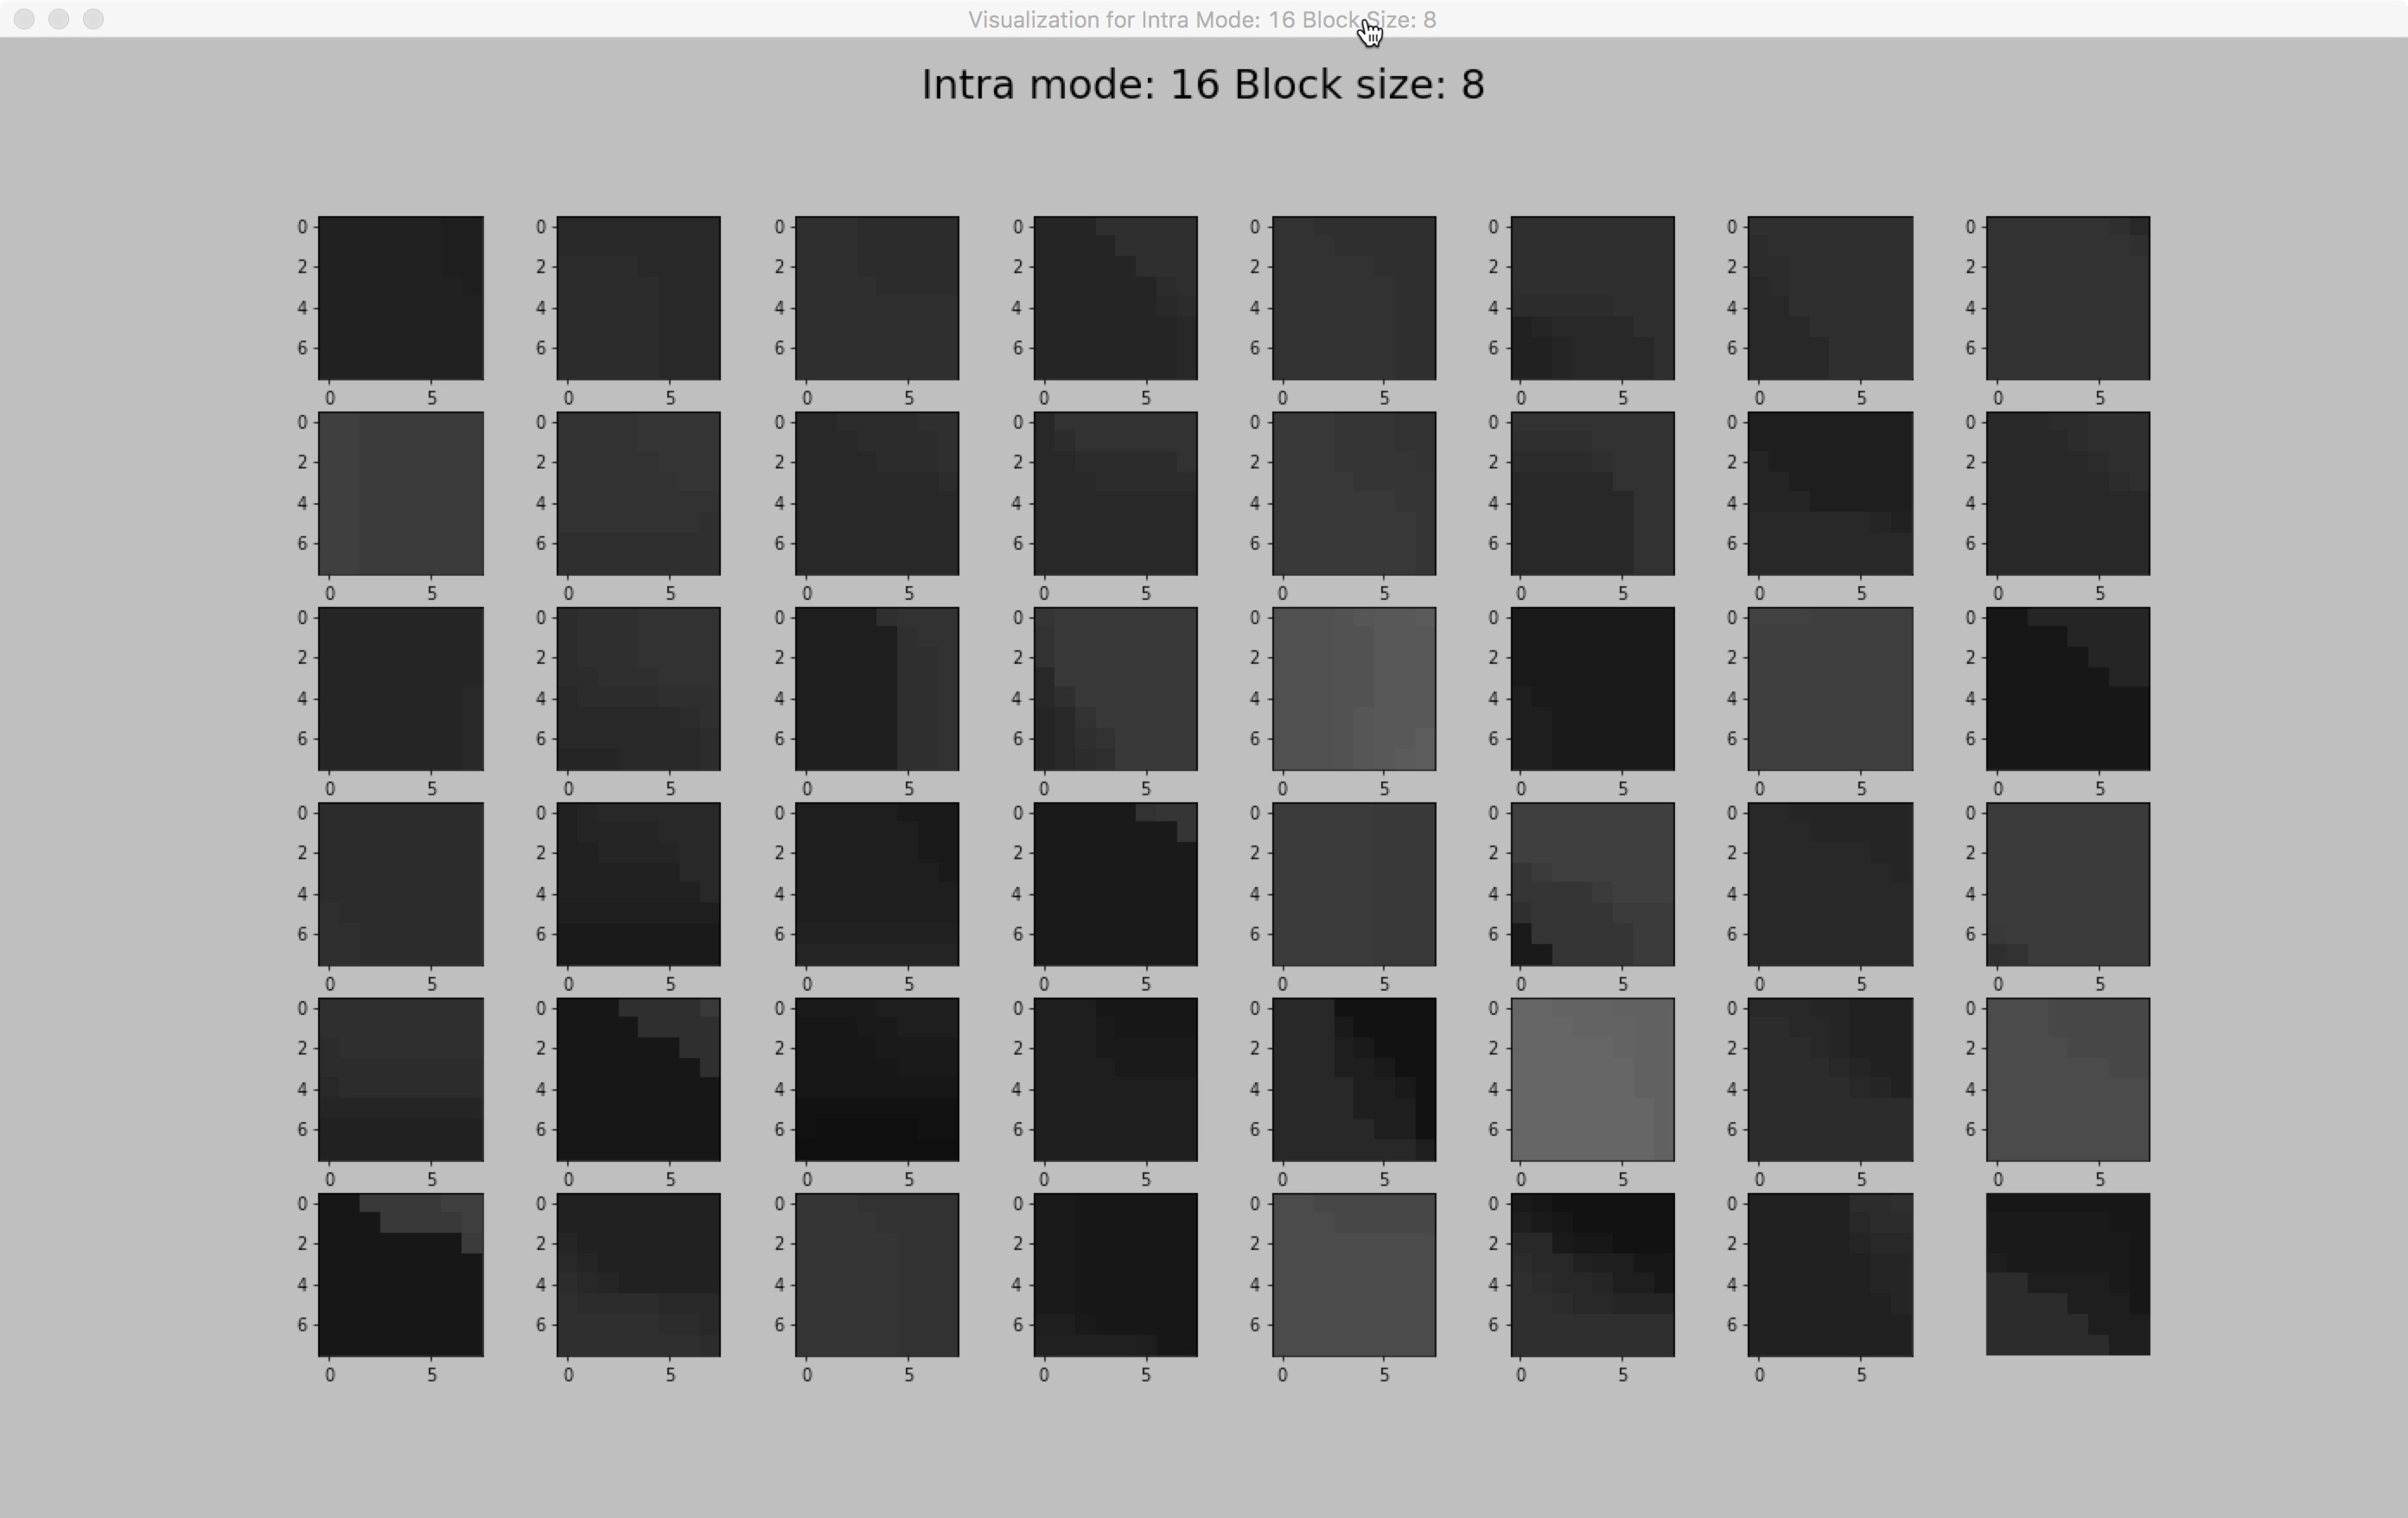
\includegraphics[width=\linewidth]{Figures/visu-size8x8/8-16}
            \caption[Visualizations for blocks tagged with intra mode 16]{Visualizations for blocks tagged with intra mode 16.}
            \label{fig:size8_mode16}
        \end{minipage}
        \hspace{\fill} % note: no blank line here
        \begin{minipage}{0.49\textwidth}
            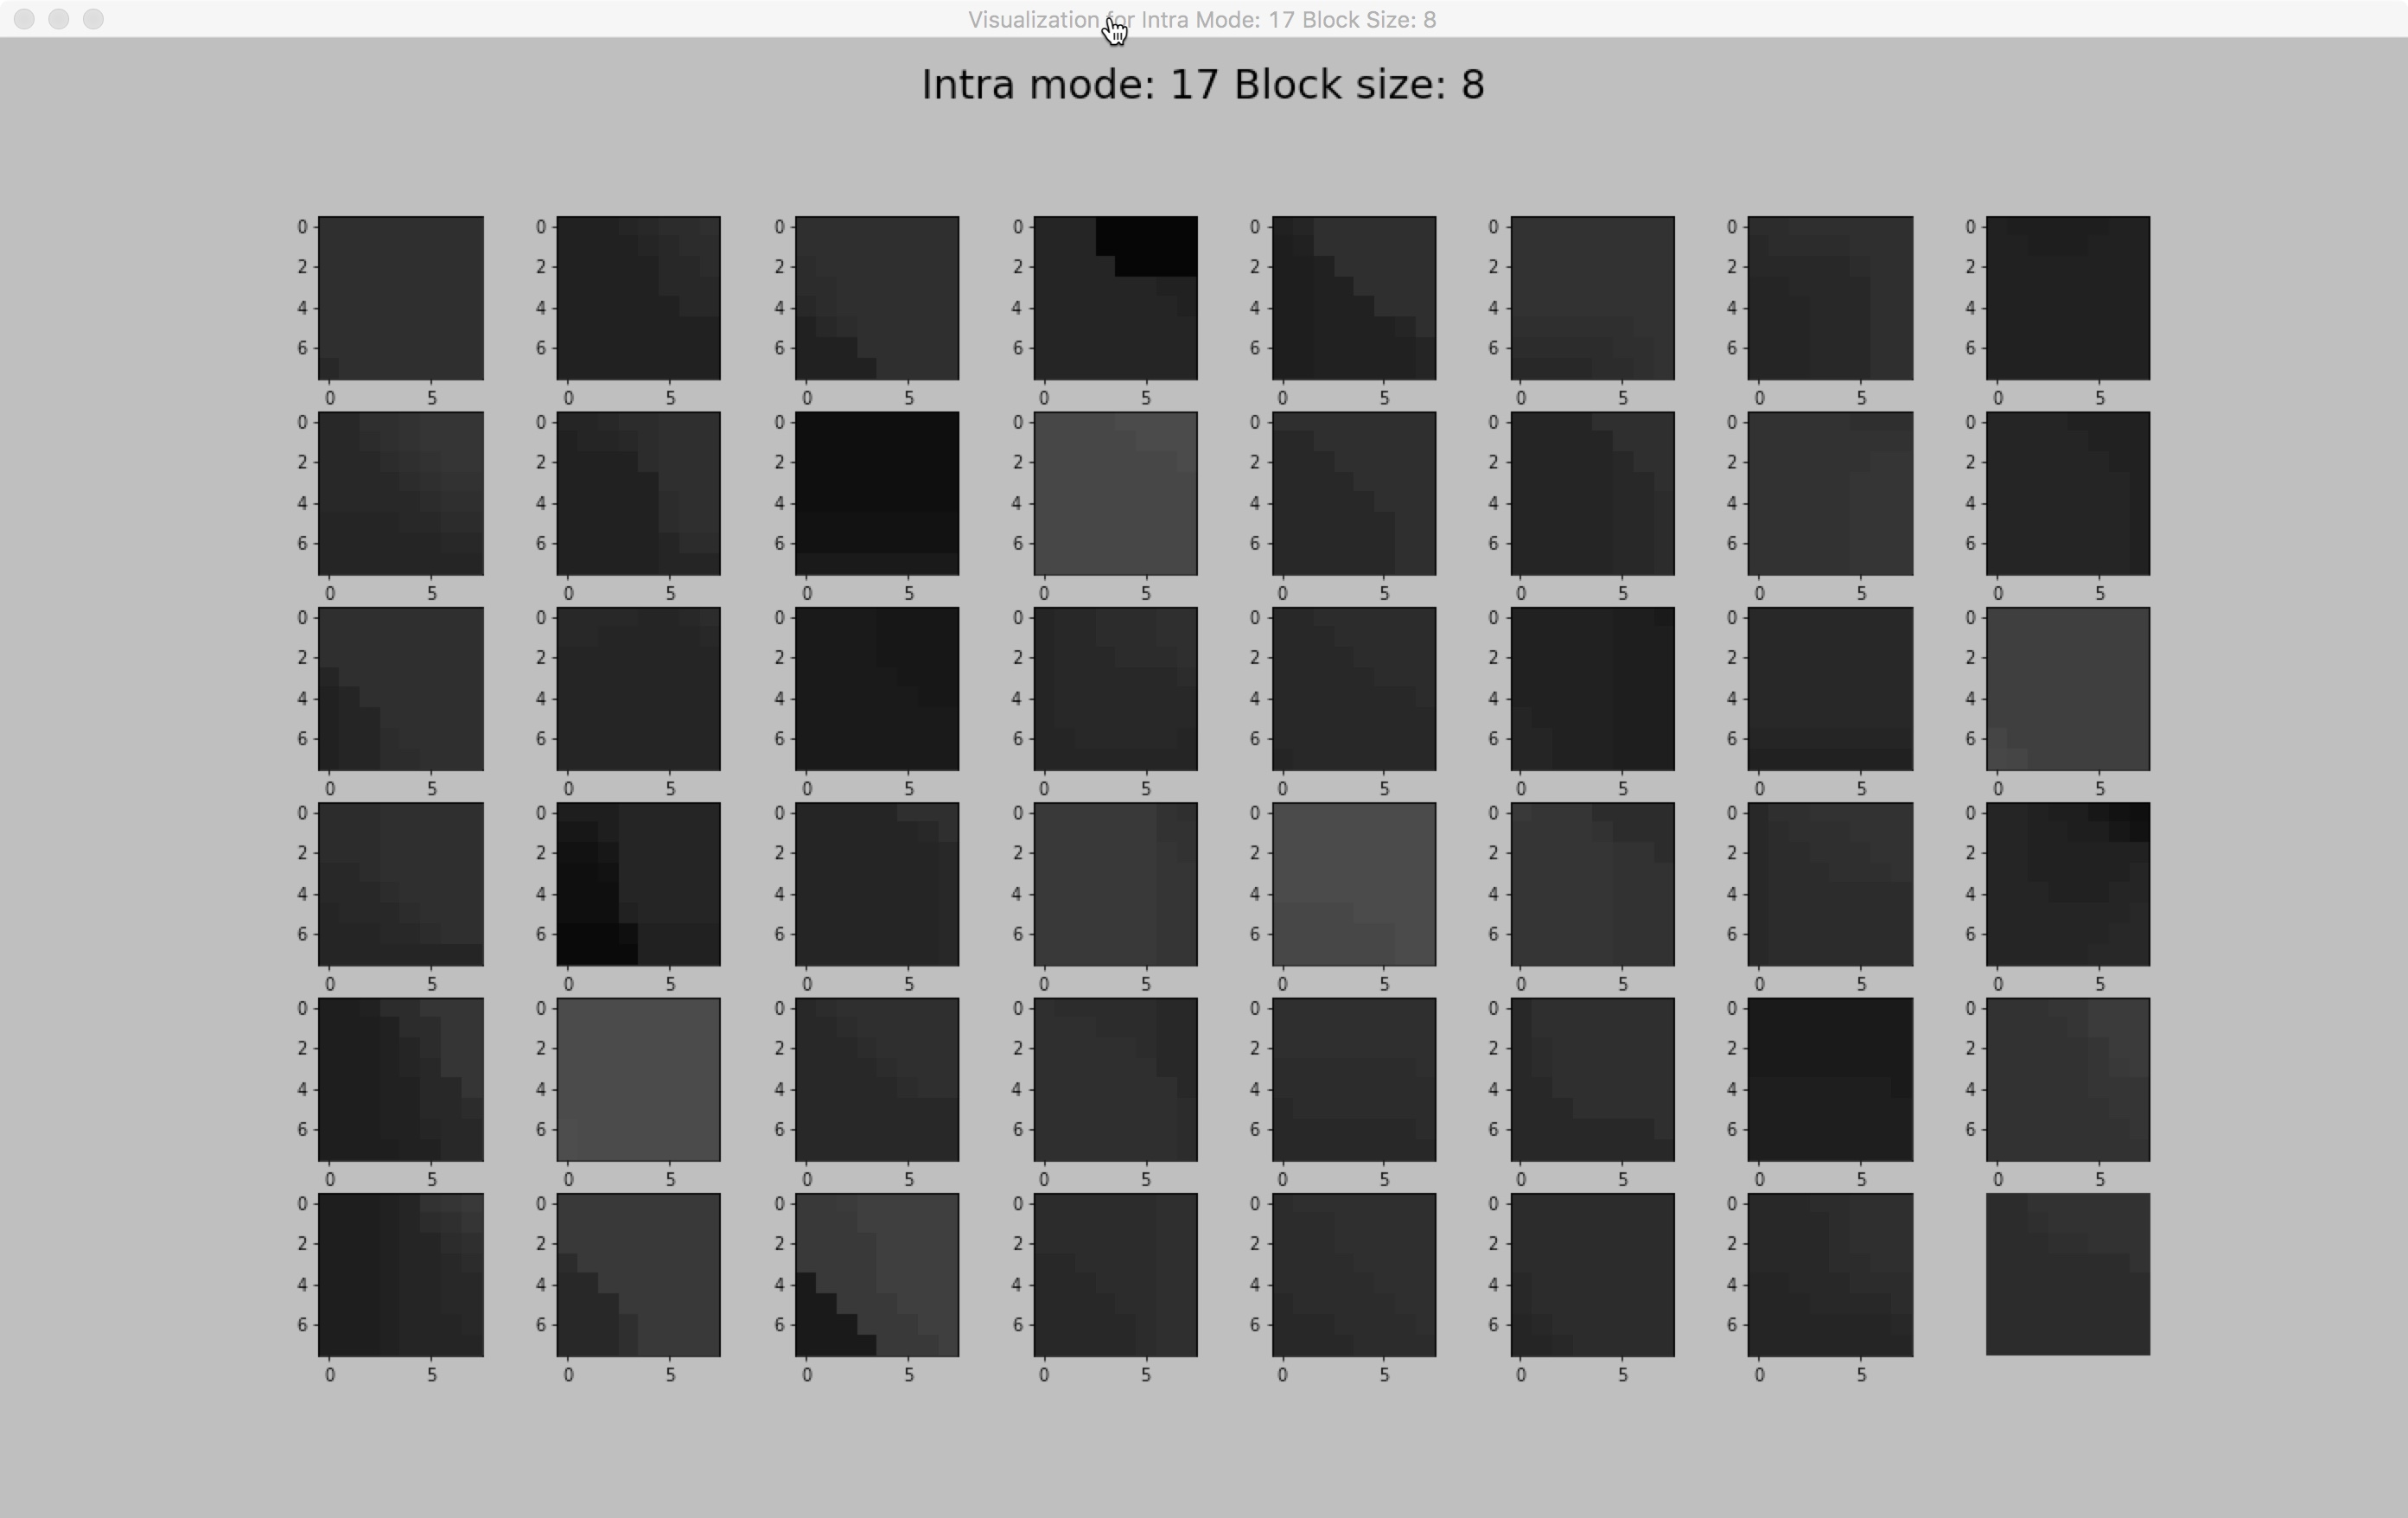
\includegraphics[width=\linewidth]{Figures/visu-size8x8/8-17}
            \caption[Visualizations for blocks tagged with intra mode 17]{Visualizations for blocks tagged with intra mode 17.}
            \label{fig:size8_mode17}
        \end{minipage}
    
        \vspace*{1cm} % vertical separation
    
        \begin{minipage}{0.49\textwidth}
            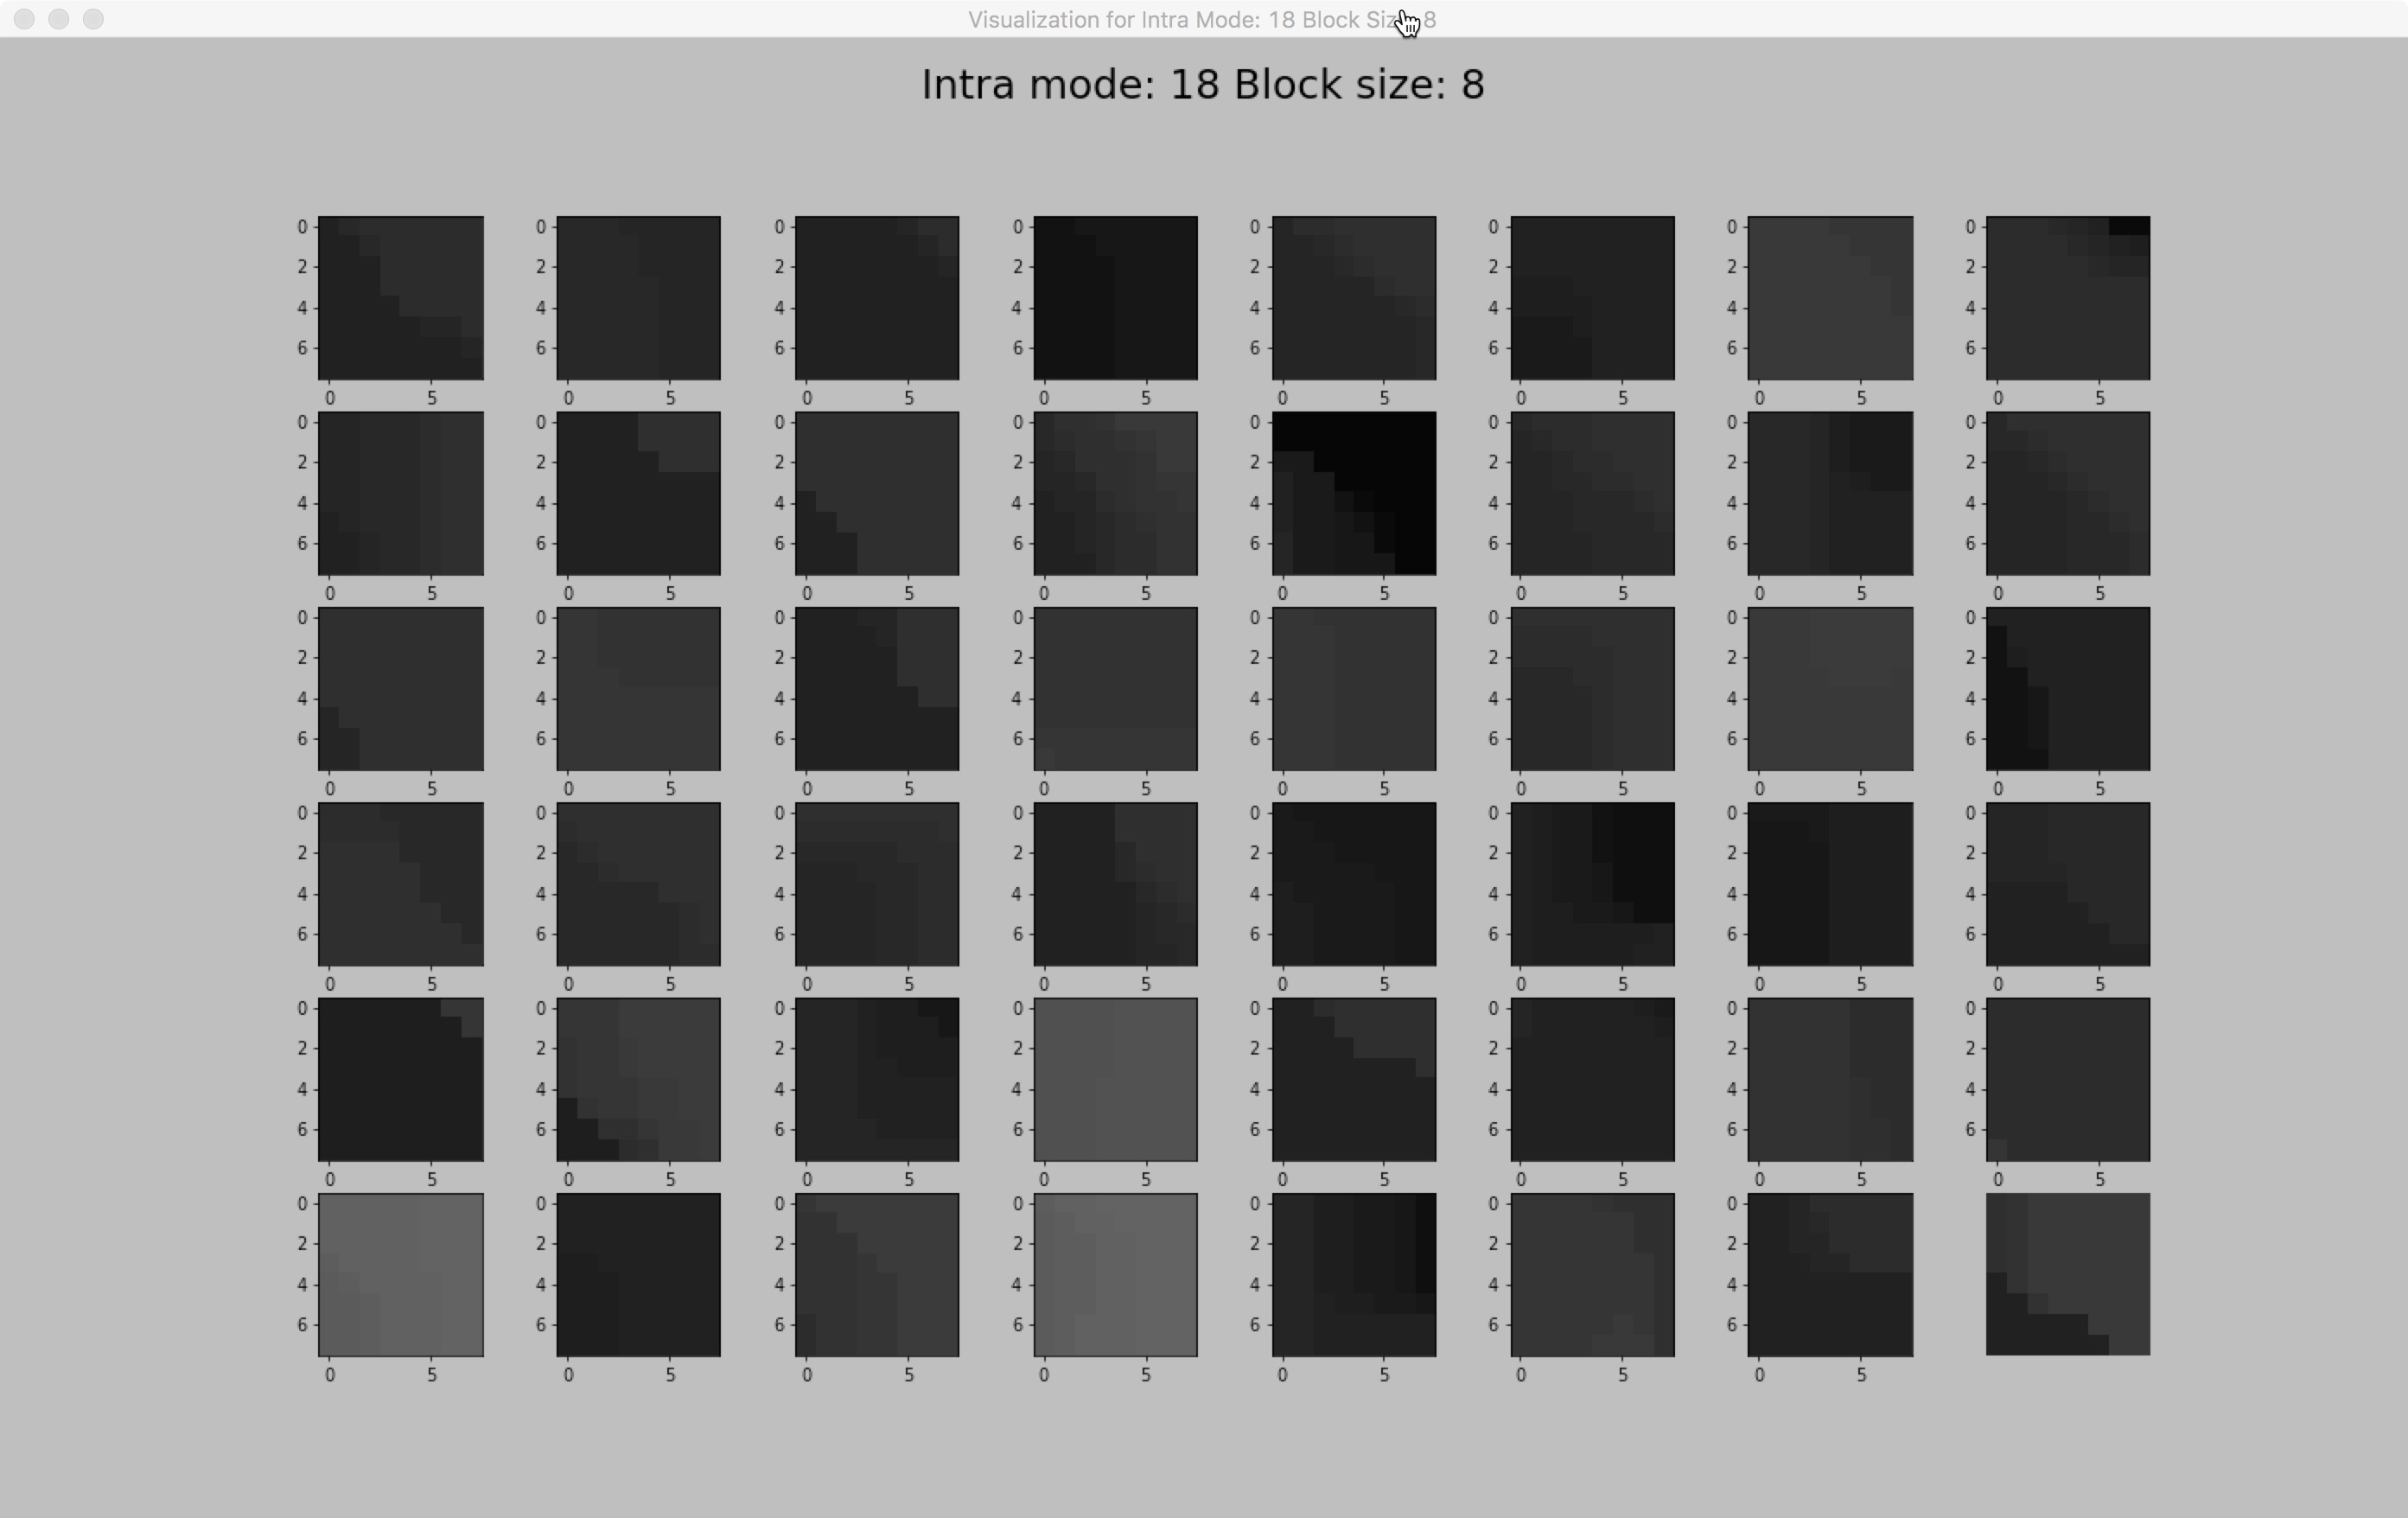
\includegraphics[width=\linewidth]{Figures/visu-size8x8/8-18}
            \caption[Visualizations for blocks tagged with intra mode 18]{Visualizations for blocks tagged with intra mode 18.}
            \label{fig:size8_mode18}
        \end{minipage}
        \hspace{\fill} % note: no blank line here
        \begin{minipage}{0.49\textwidth}
            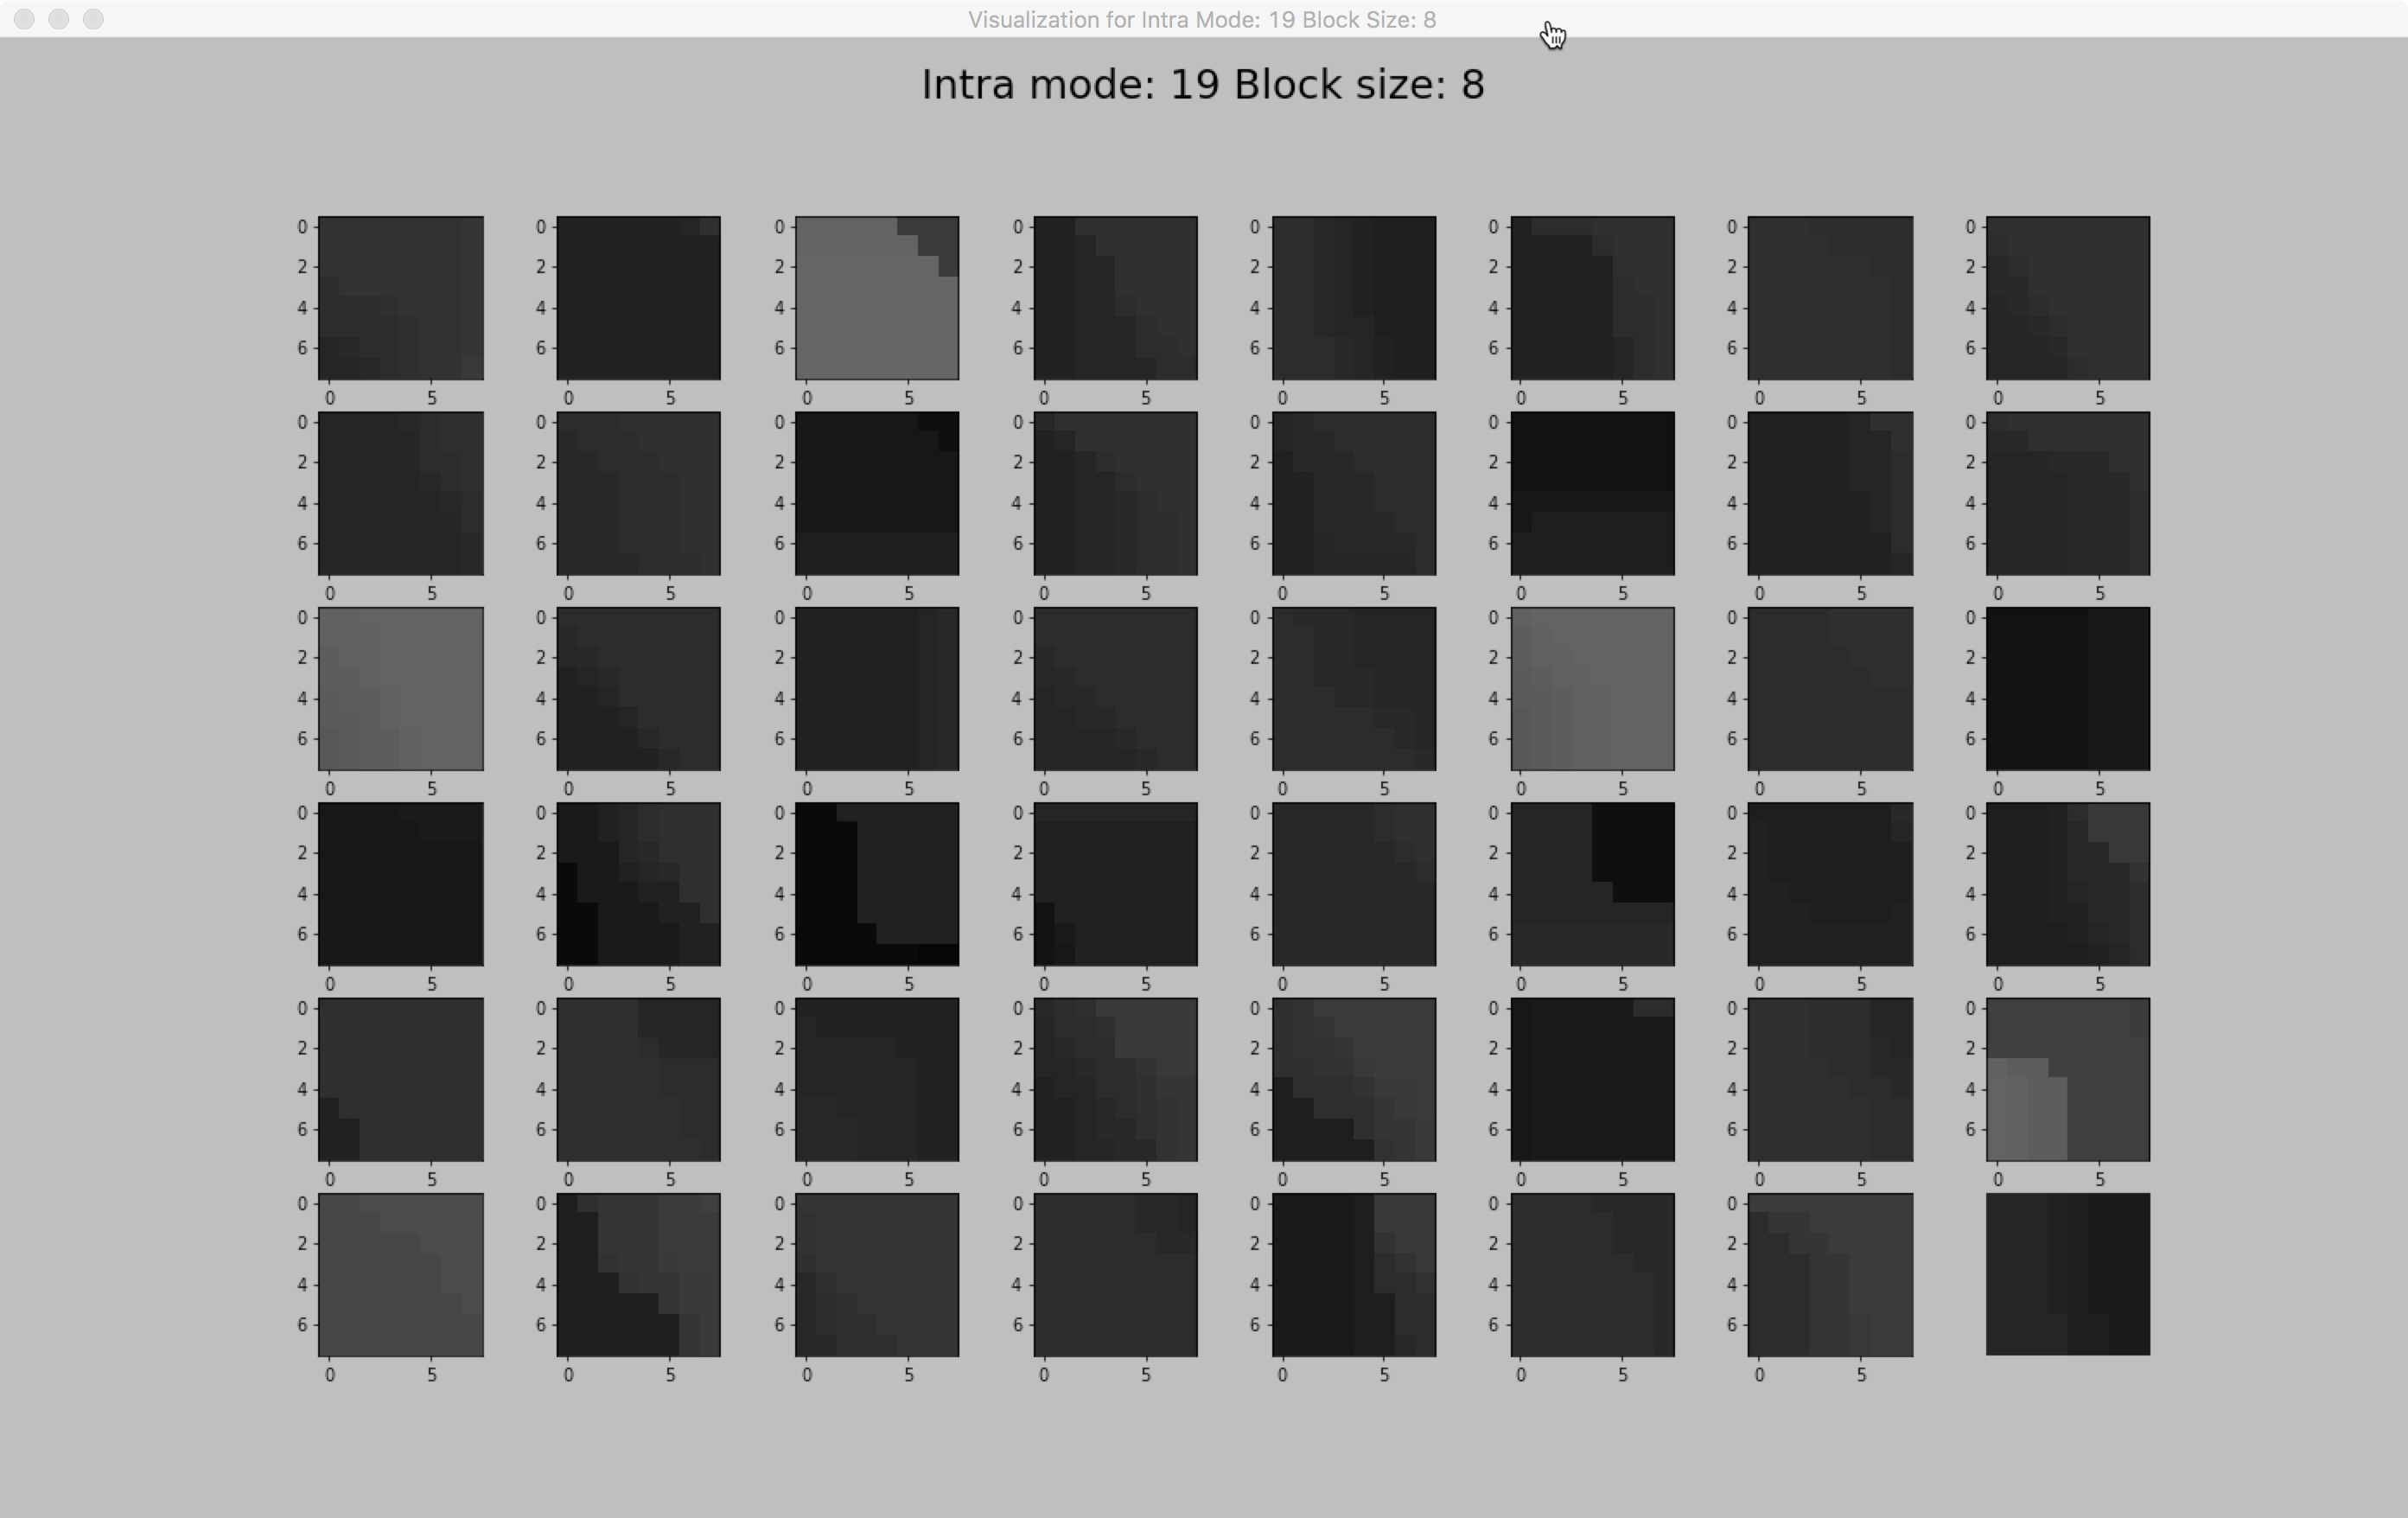
\includegraphics[width=\linewidth]{Figures/visu-size8x8/8-19}
            \caption[Visualizations for blocks tagged with intra mode 19]{Visualizations for blocks tagged with intra mode 19.}
            \label{fig:size8_mode19}
        \end{minipage}
        
        \vspace*{1cm} % vertical separation
    
        \begin{minipage}{0.49\textwidth}
            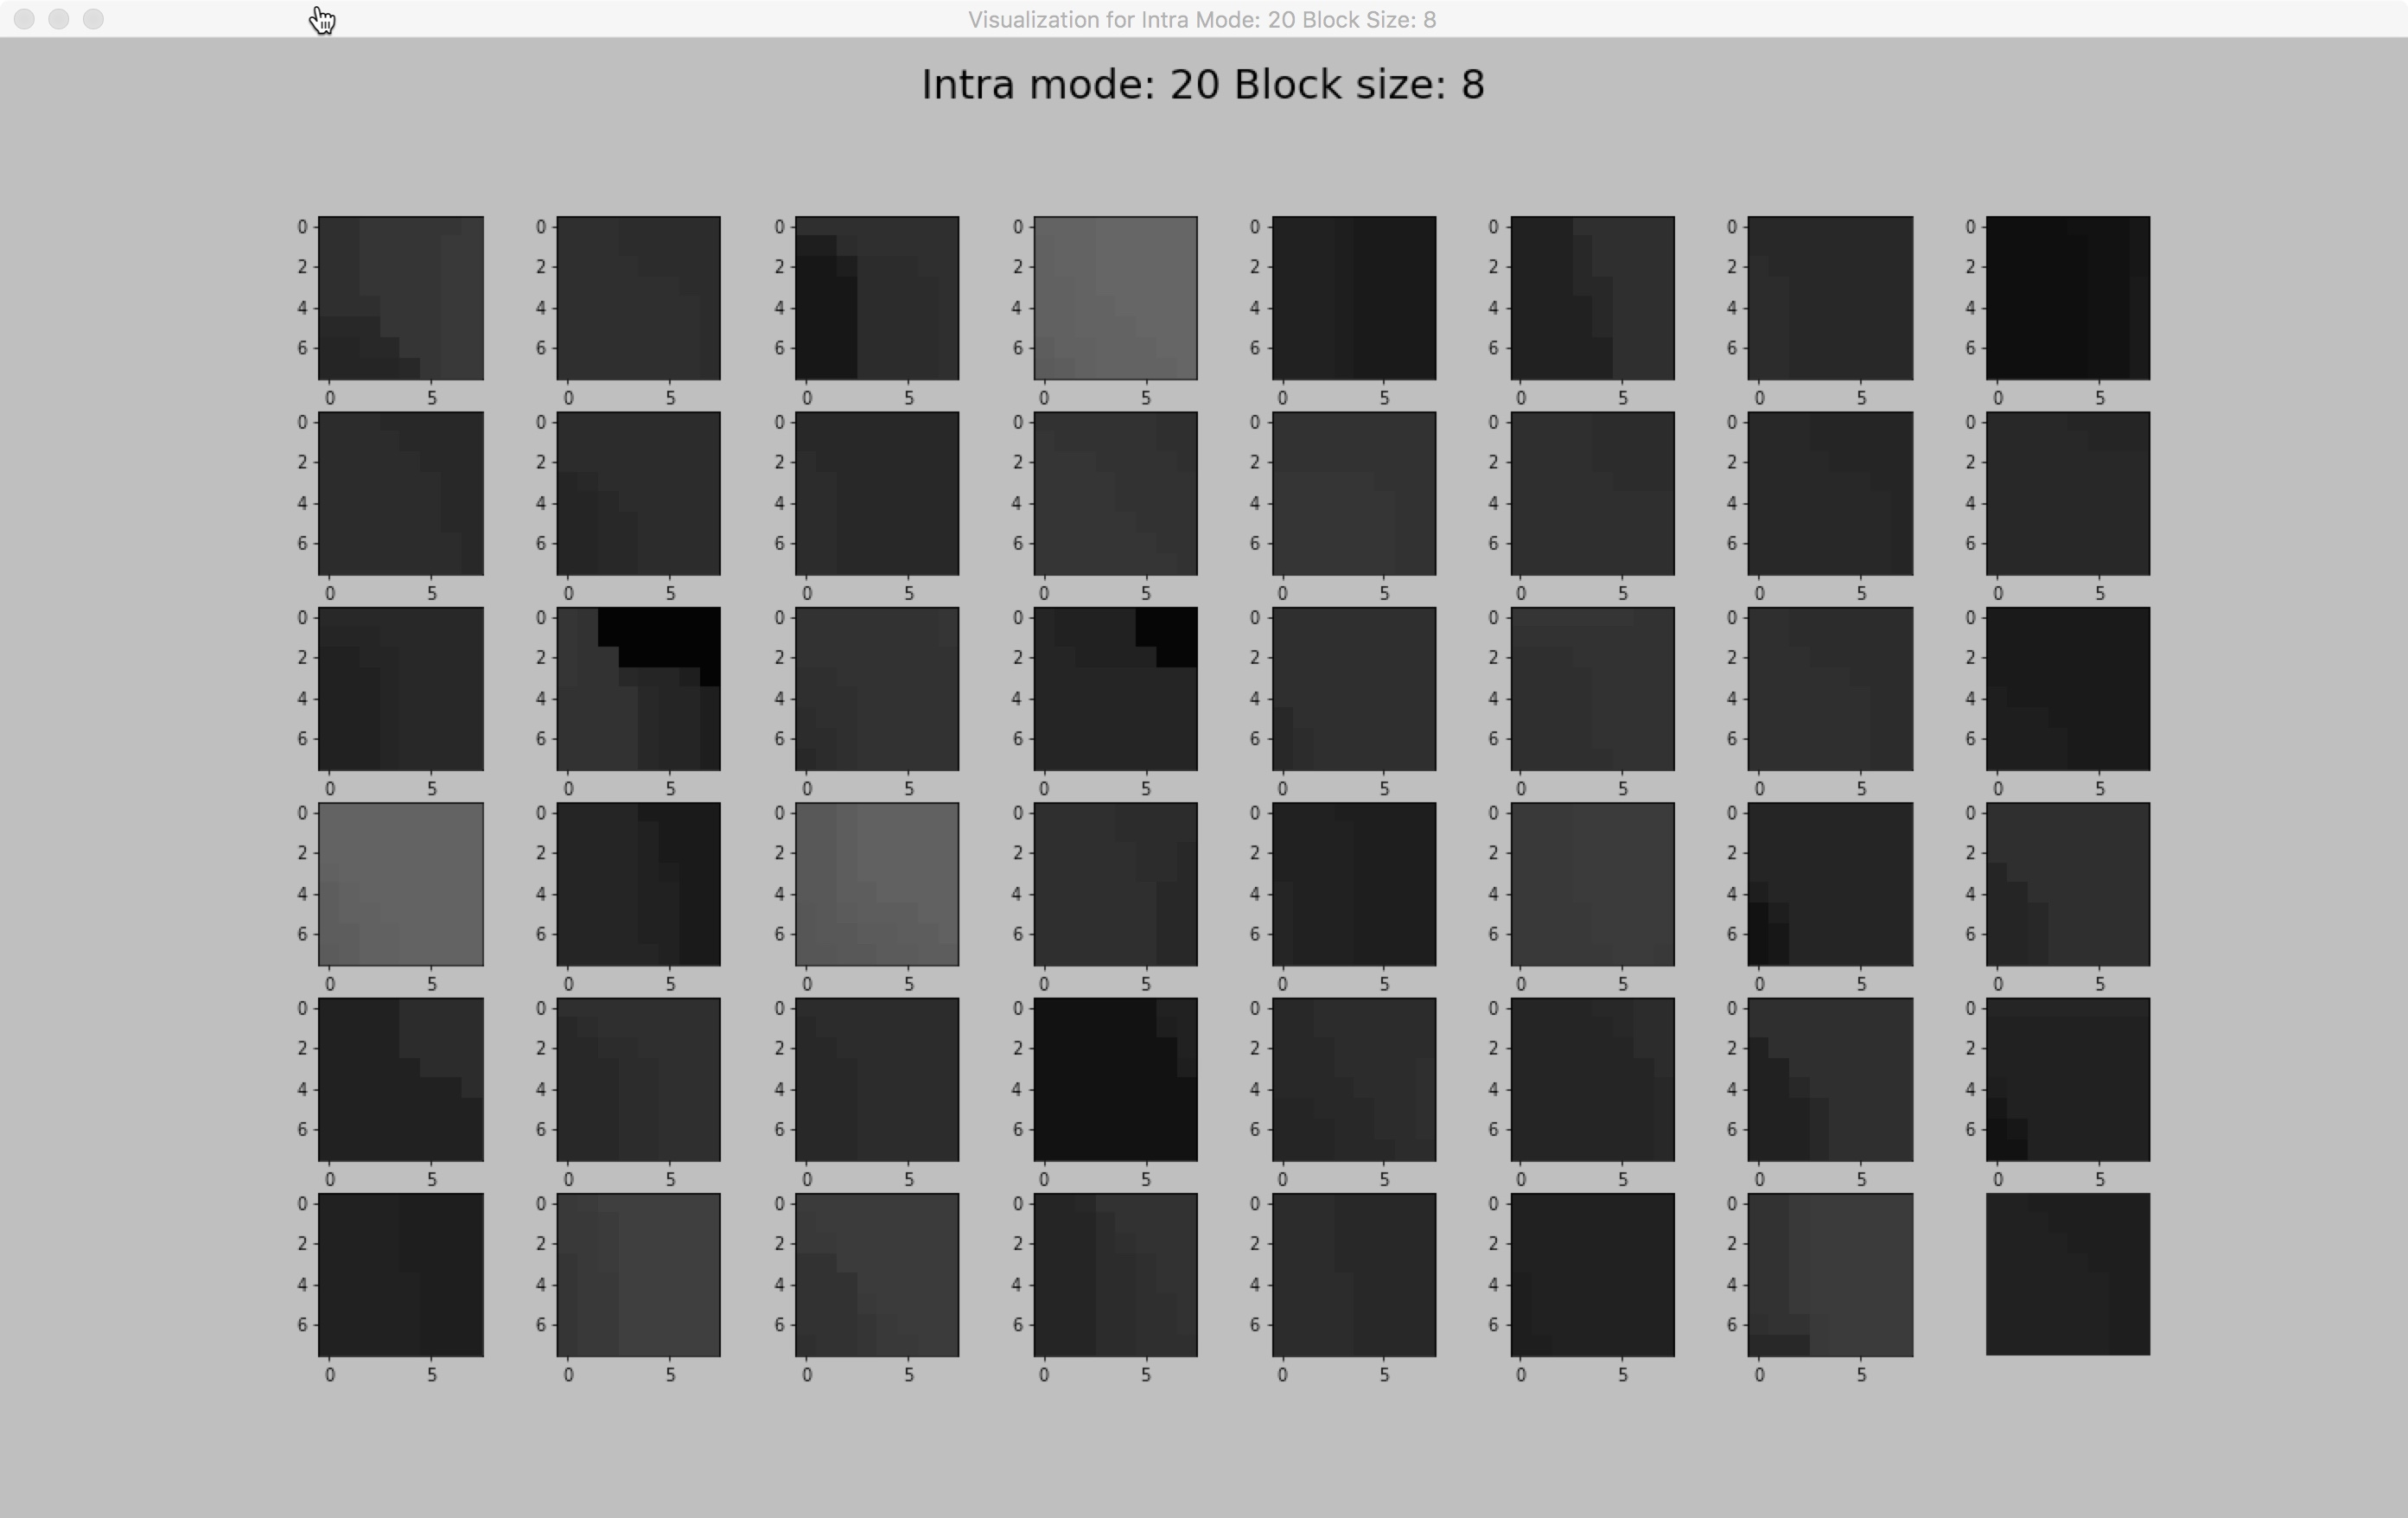
\includegraphics[width=\linewidth]{Figures/visu-size8x8/8-20}
            \caption[Visualizations for blocks tagged with intra mode 20]{Visualizations for blocks tagged with intra mode 20.}
            \label{fig:size8_mode20}
        \end{minipage}
        \hspace{\fill} % note: no blank line here
        \begin{minipage}{0.49\textwidth}
            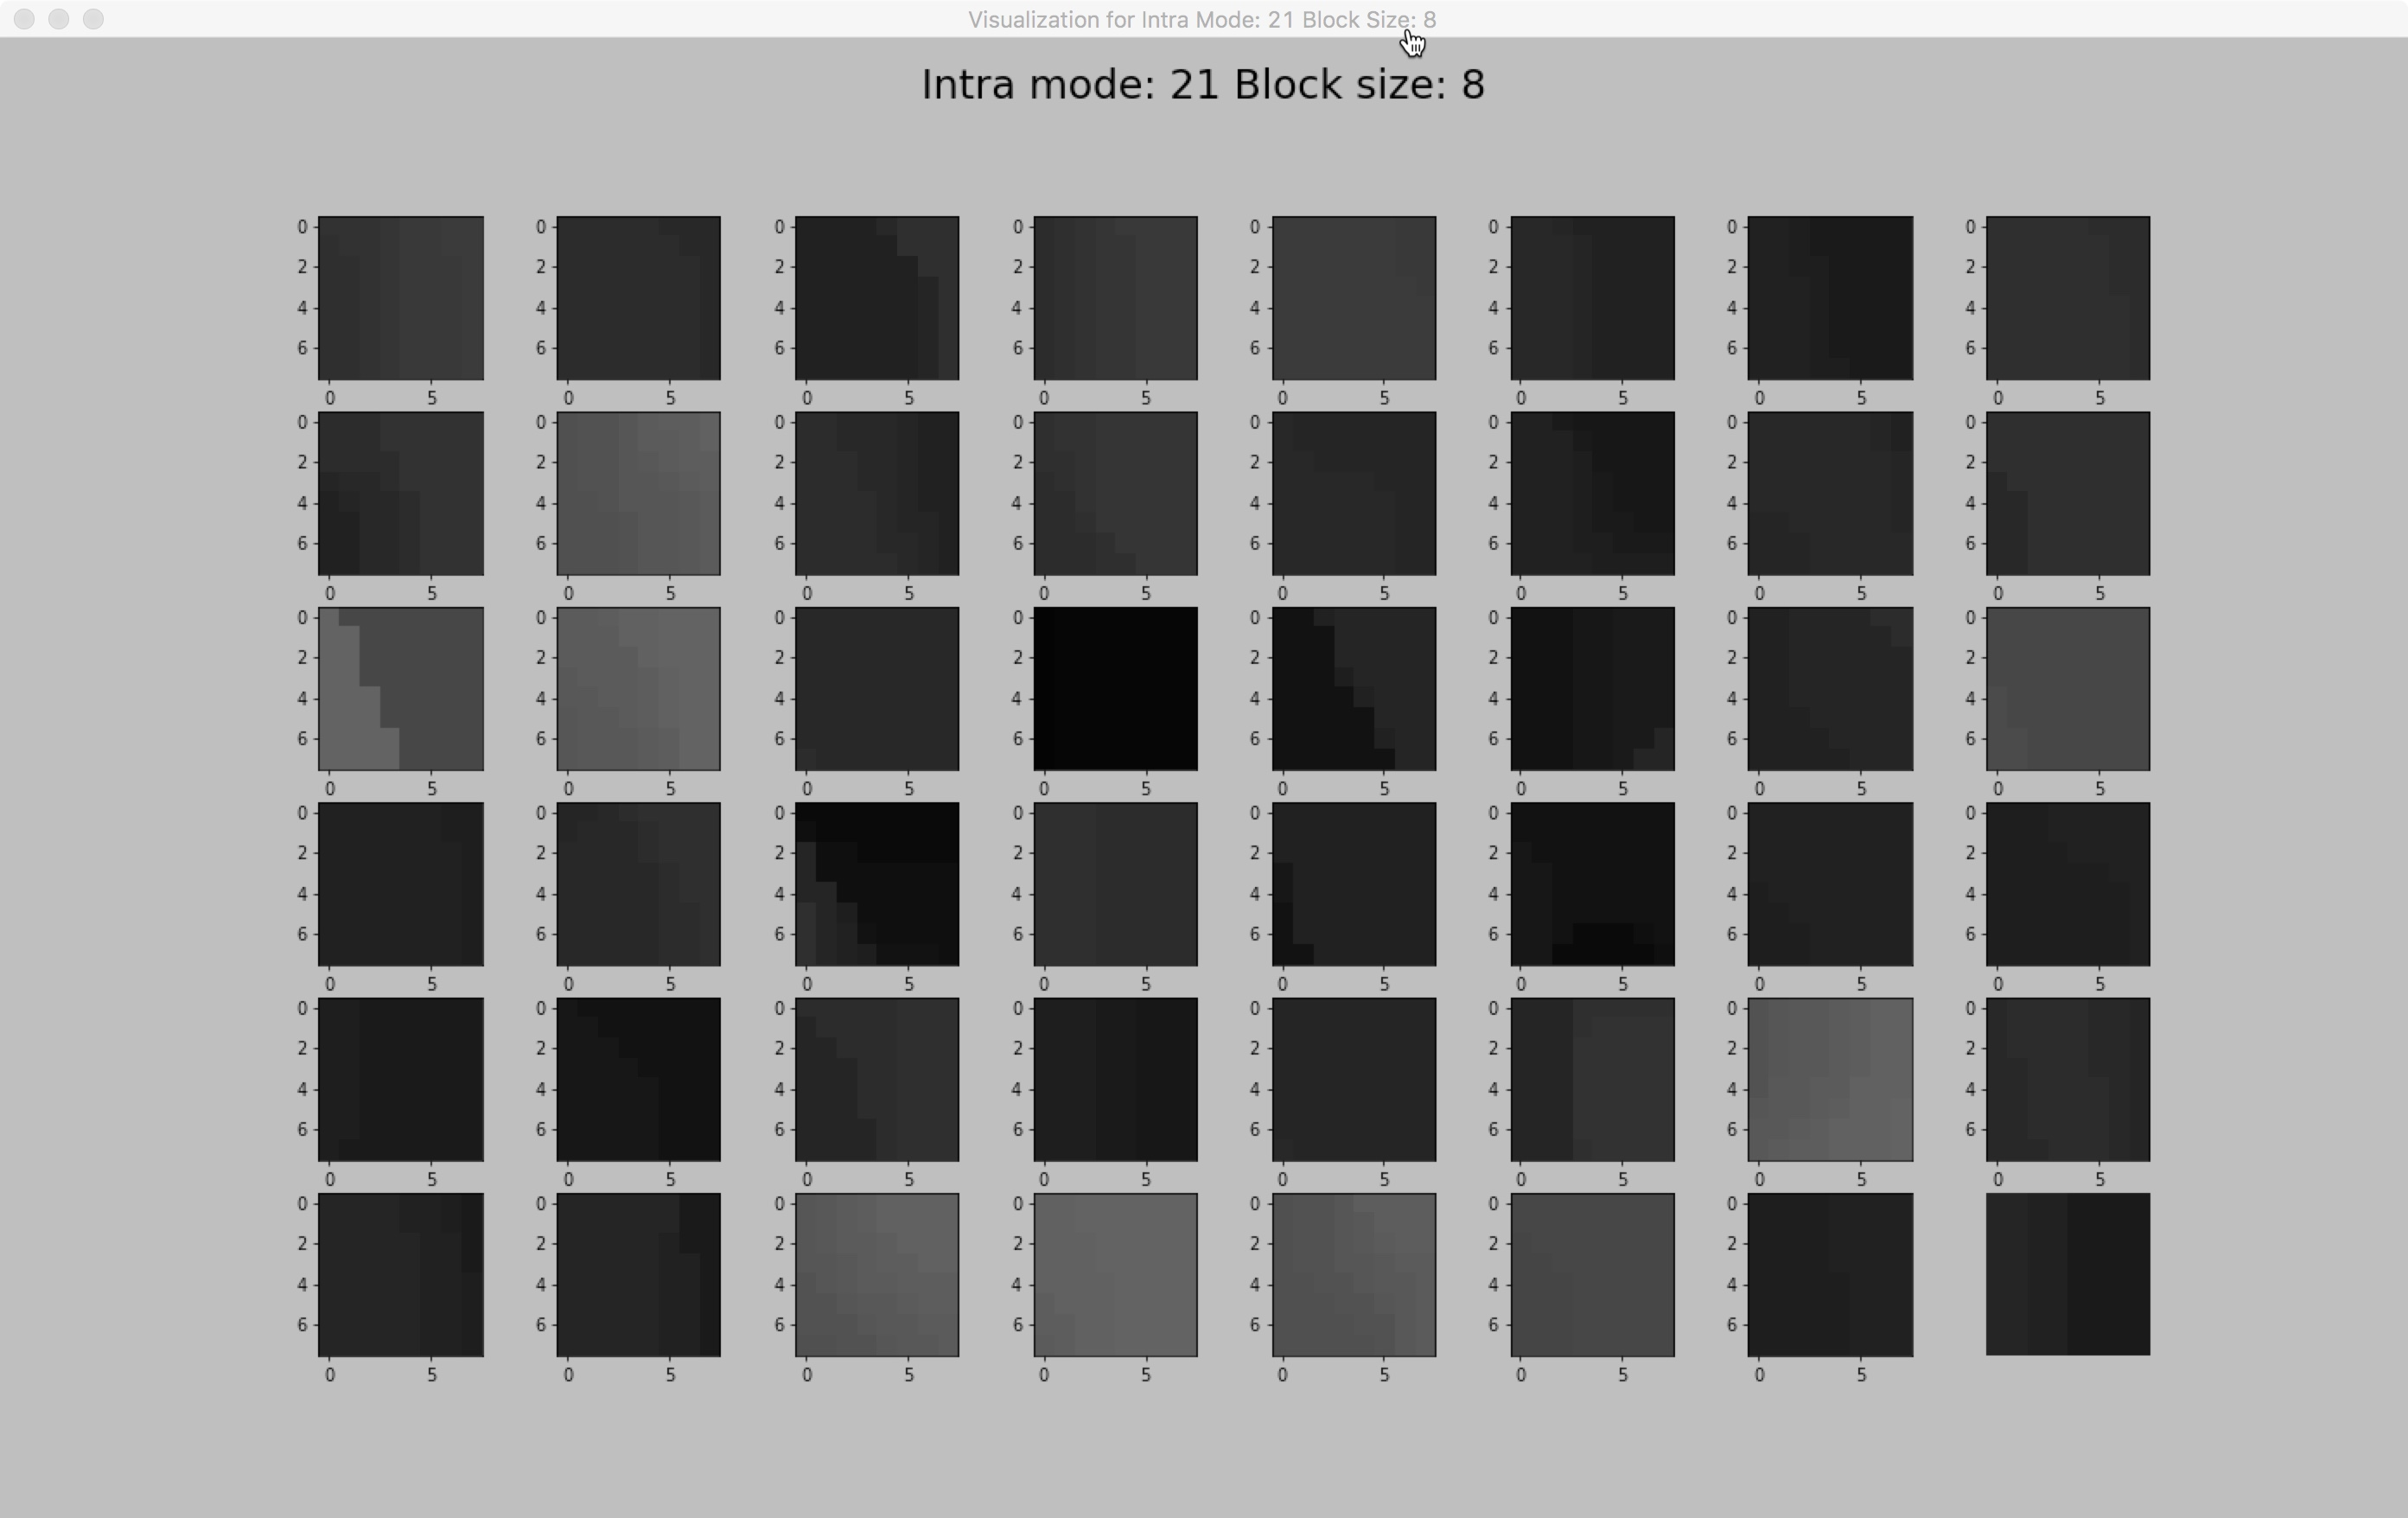
\includegraphics[width=\linewidth]{Figures/visu-size8x8/8-21}
            \caption[Visualizations for blocks tagged with intra mode 21]{Visualizations for blocks tagged with intra mode 21.}
            \label{fig:size8_mode21}
        \end{minipage}
    
    % \caption{Figure caption goes here}\label{fig:see-data-visu}
    \end{figure}
    
    \begin{figure}
    
        \vspace*{1cm} % vertical separation
    
        \begin{minipage}{0.49\textwidth}
            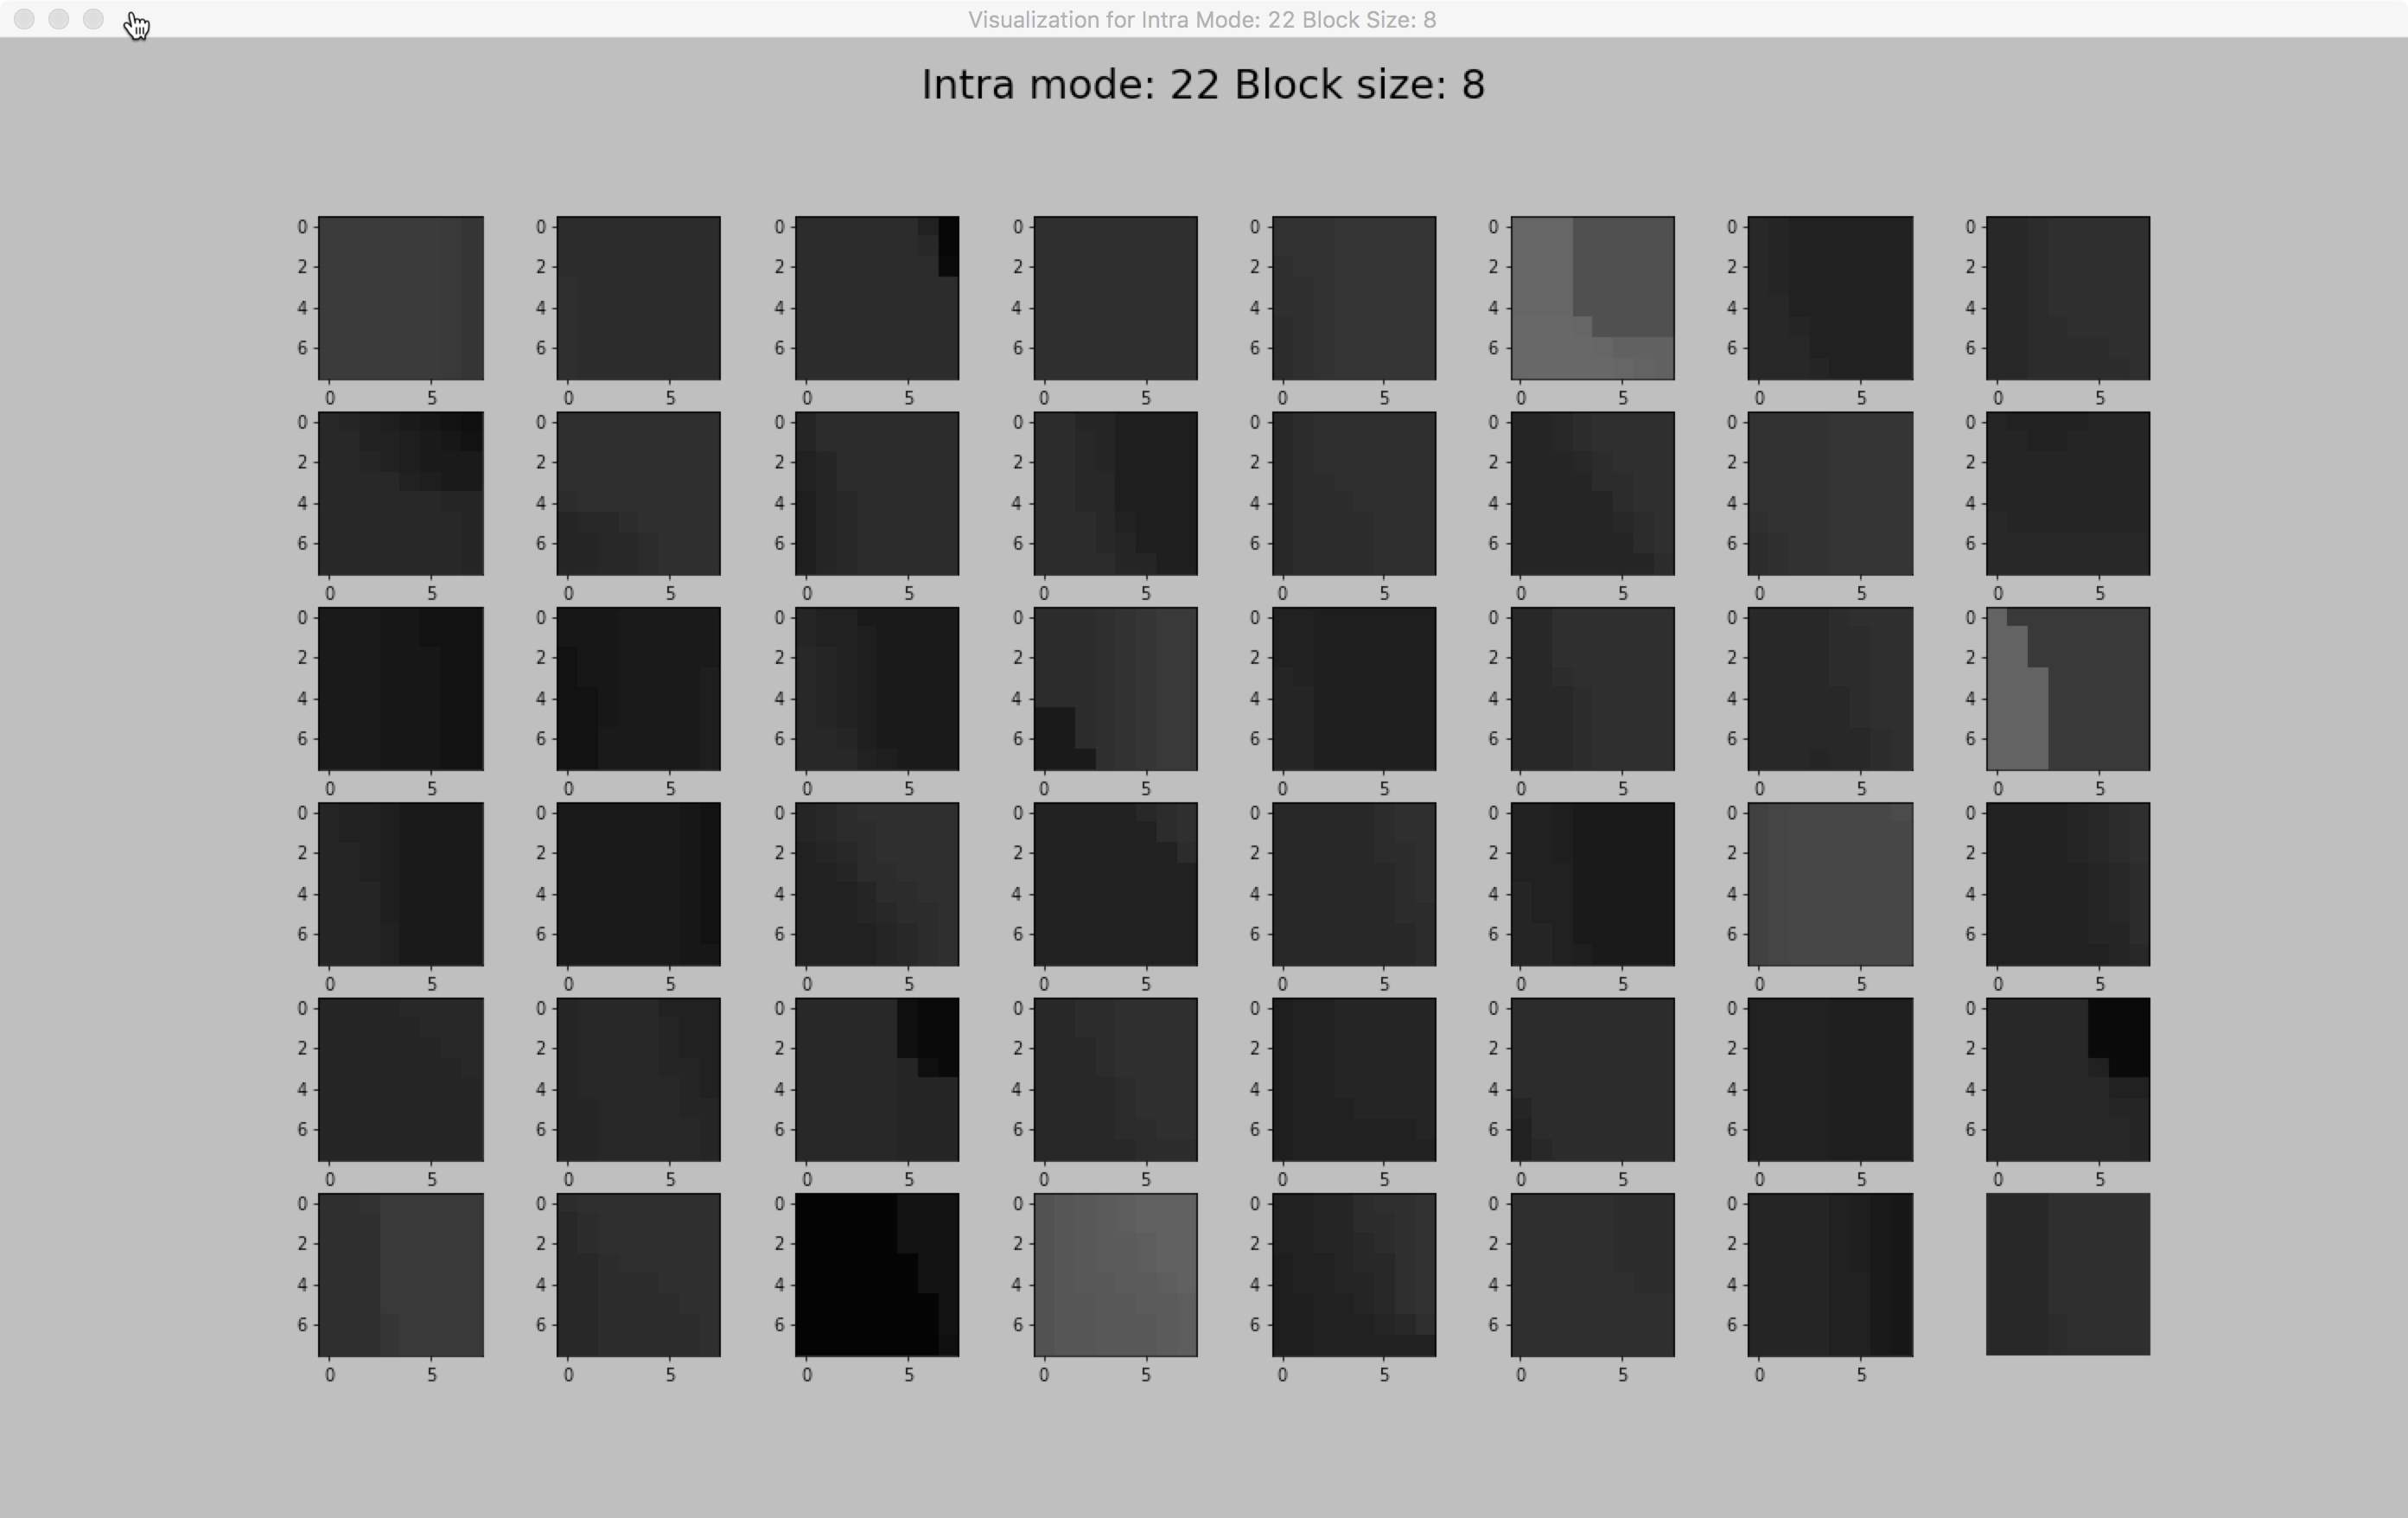
\includegraphics[width=\linewidth]{Figures/visu-size8x8/8-22}
            \caption[Visualizations for blocks tagged with intra mode 22]{Visualizations for blocks tagged with intra mode 22.}
            \label{fig:size8_mode22}
        \end{minipage}
        \hspace{\fill} % note: no blank line here
        \begin{minipage}{0.49\textwidth}
            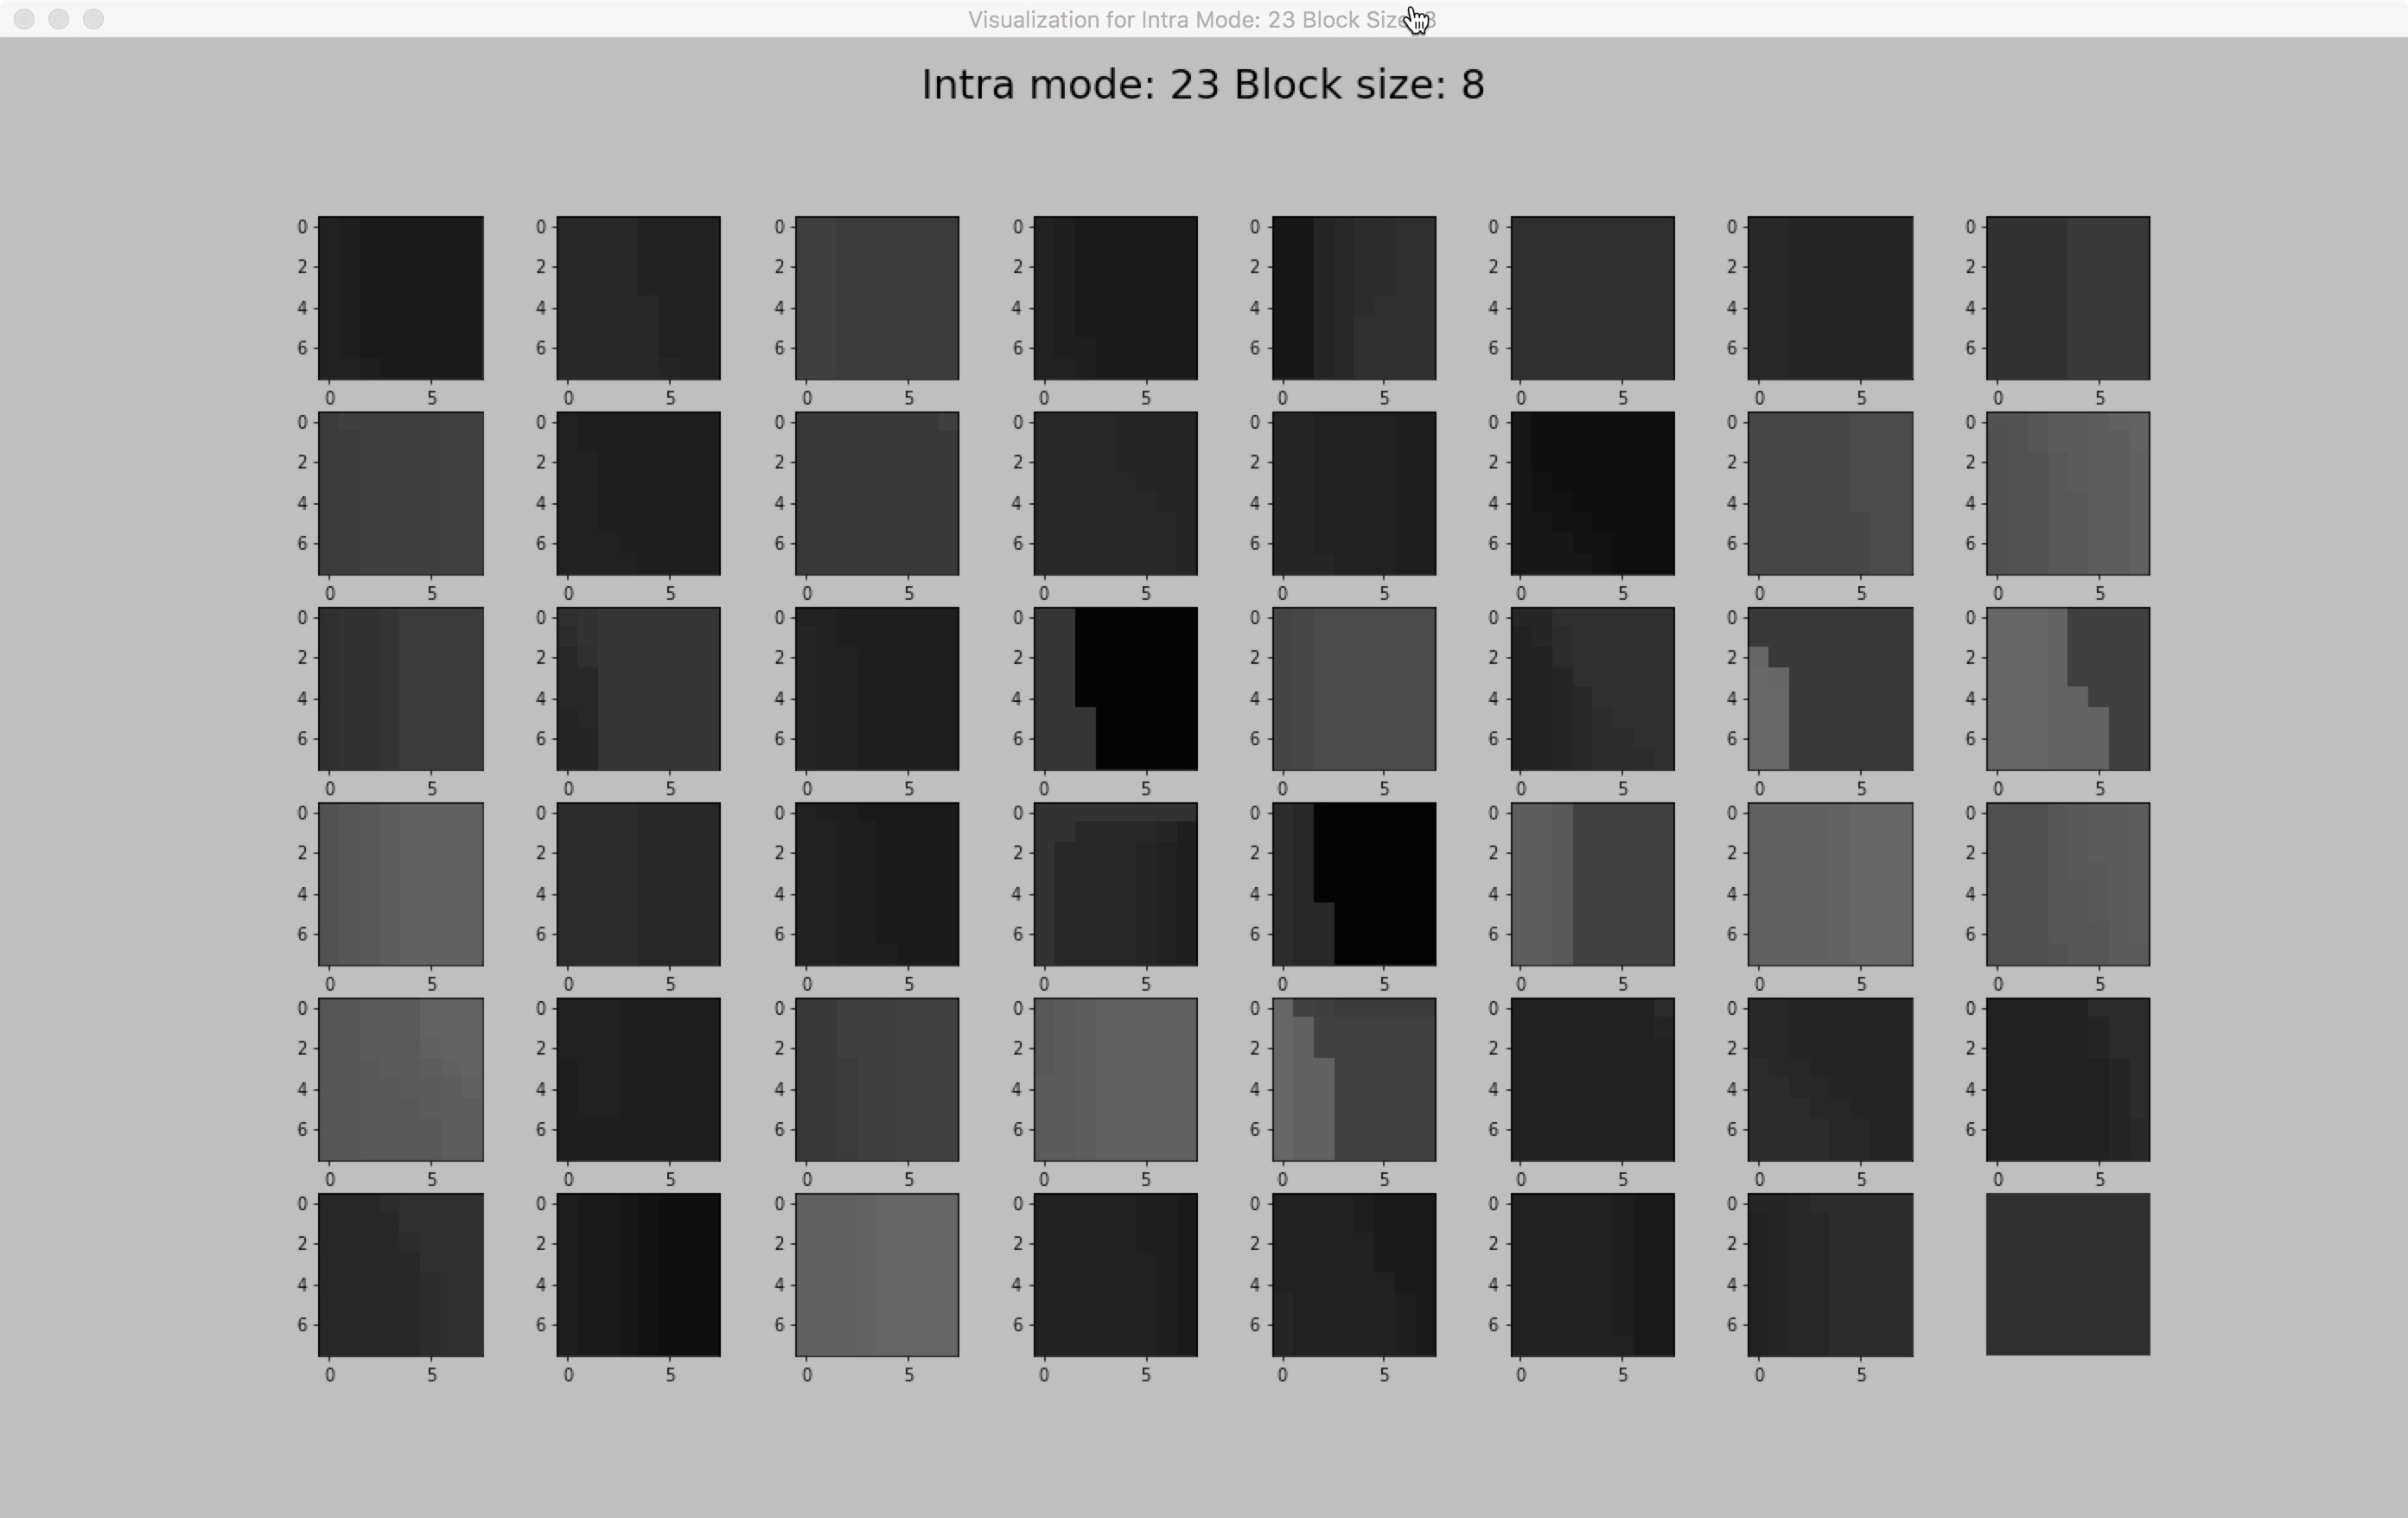
\includegraphics[width=\linewidth]{Figures/visu-size8x8/8-23}
            \caption[Visualizations for blocks tagged with intra mode 23]{Visualizations for blocks tagged with intra mode 23.}
            \label{fig:size8_mode23}
        \end{minipage}
    
        \vspace*{1cm} % vertical separation
    
        \begin{minipage}{0.49\textwidth}
            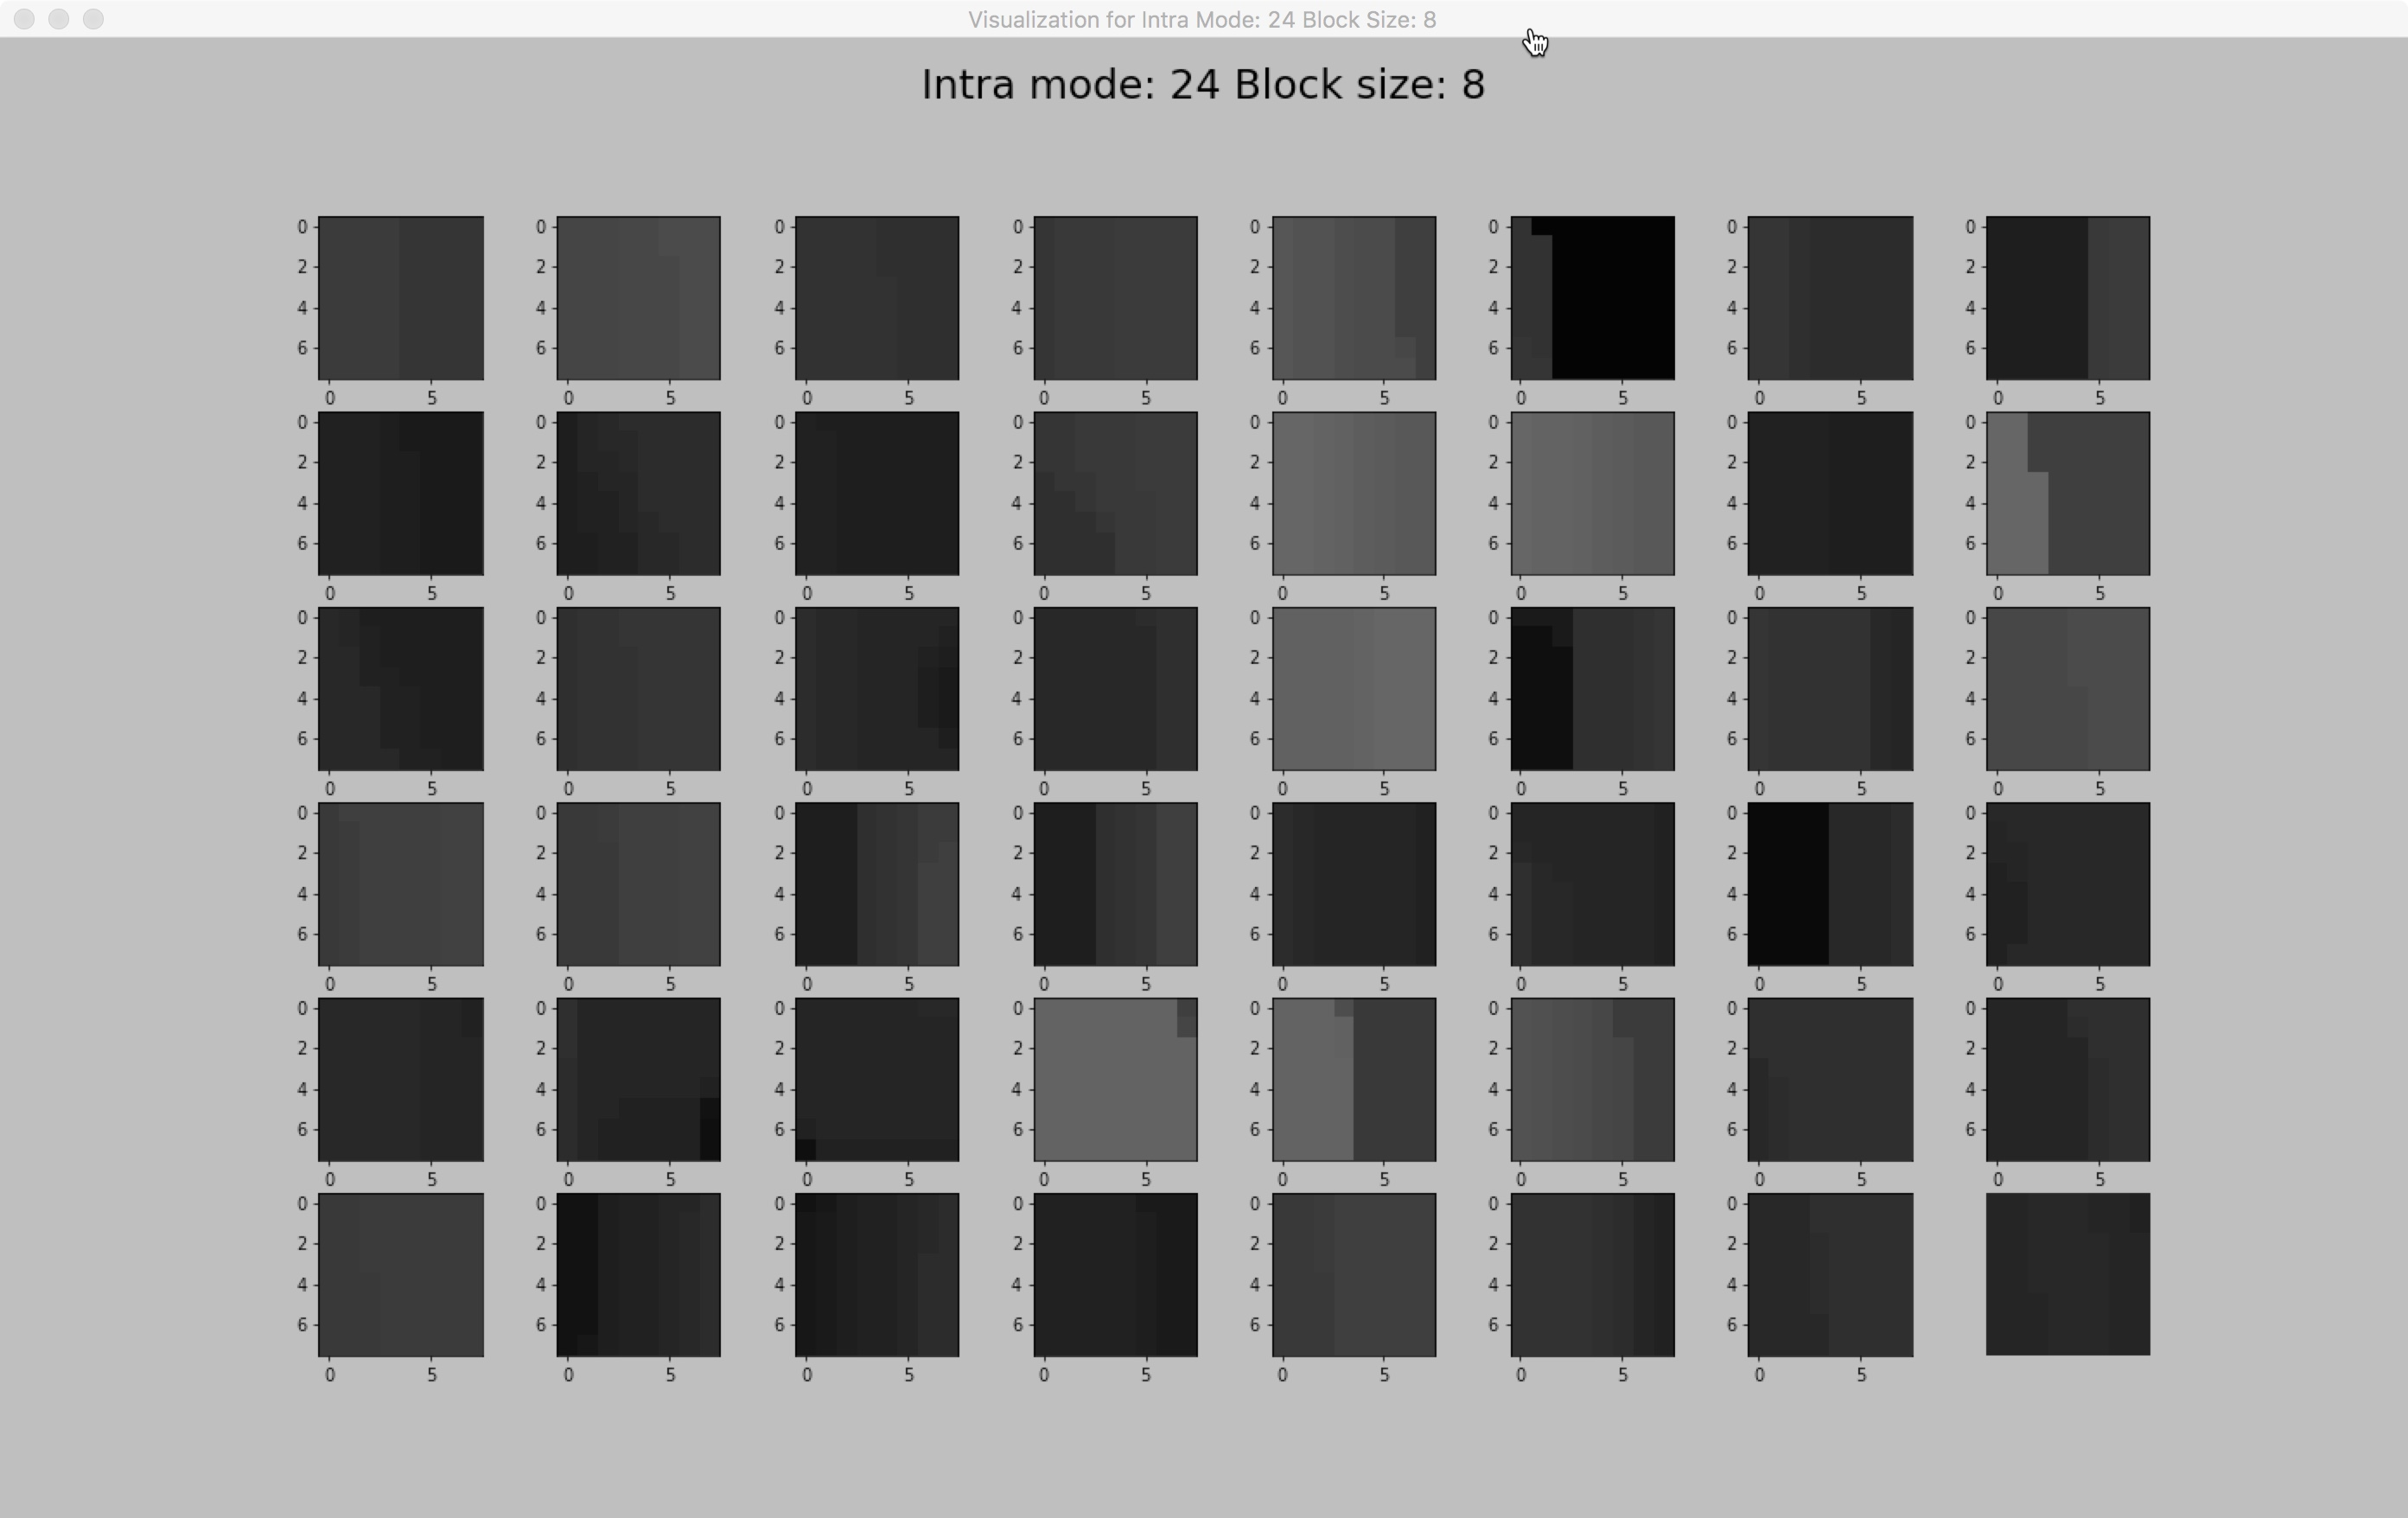
\includegraphics[width=\linewidth]{Figures/visu-size8x8/8-24}
            \caption[Visualizations for blocks tagged with intra mode 24]{Visualizations for blocks tagged with intra mode 24.}
            \label{fig:size8_mode24}
        \end{minipage}
        \hspace{\fill} % note: no blank line here
        \begin{minipage}{0.49\textwidth}
            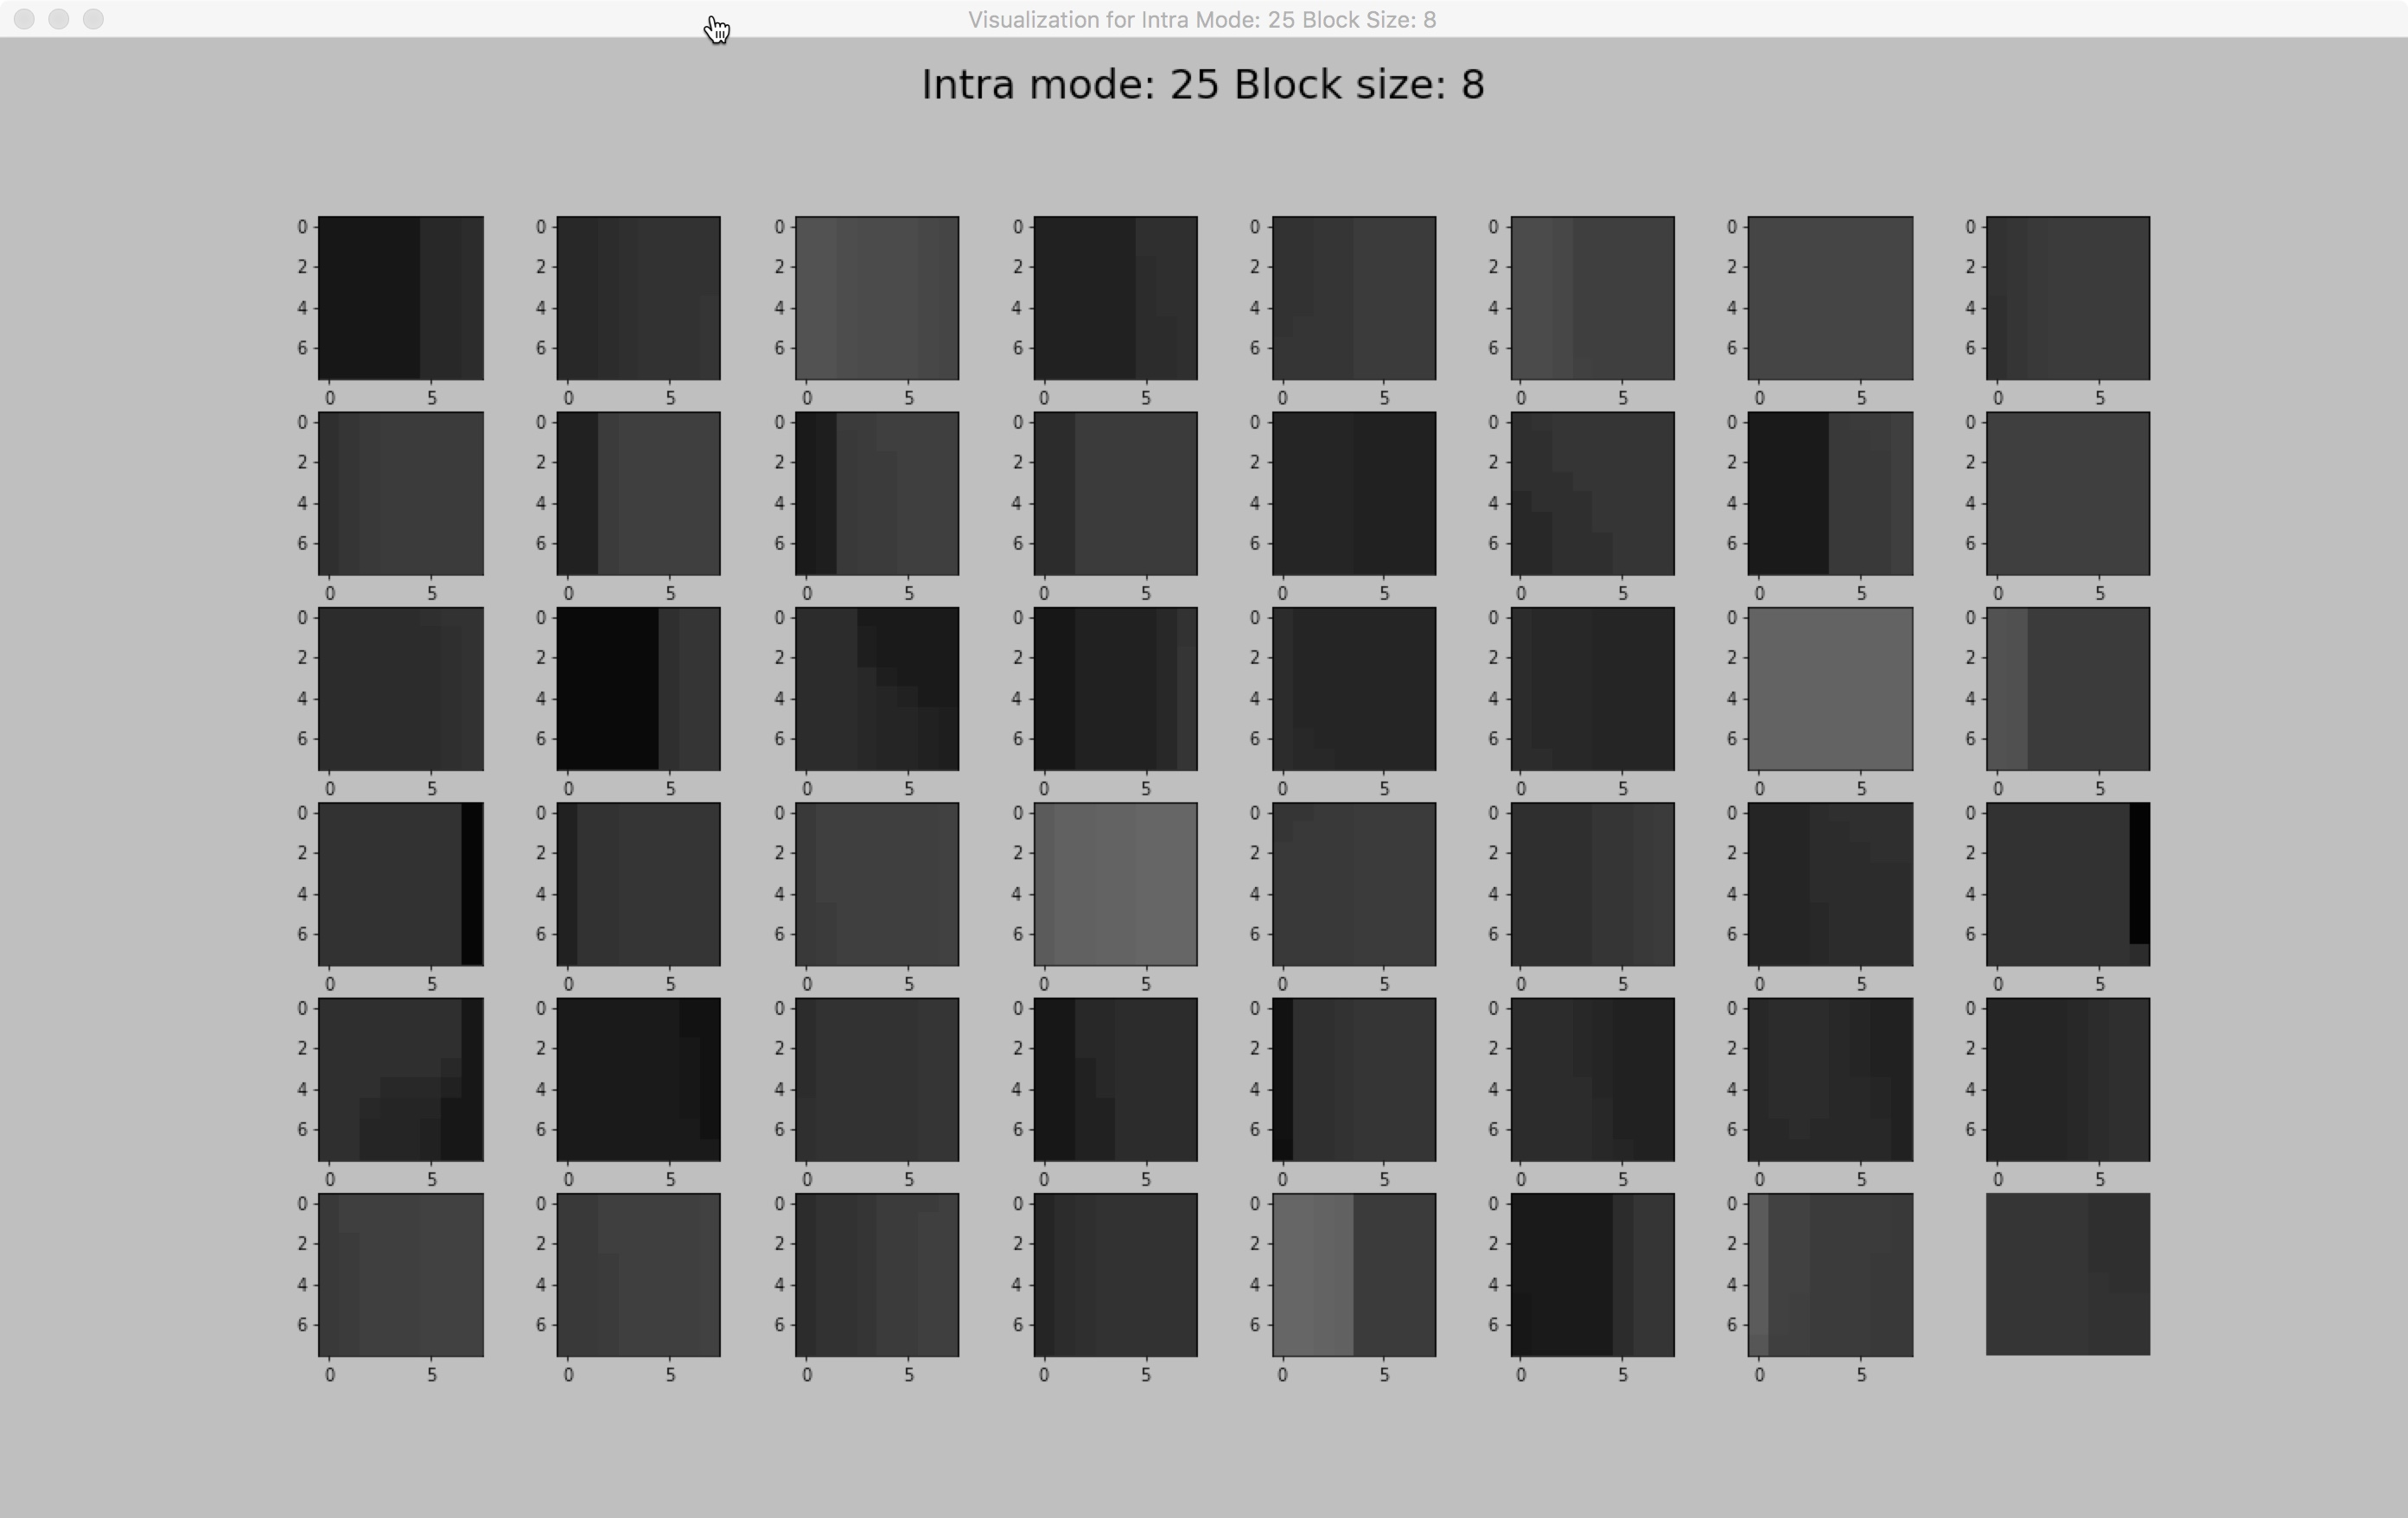
\includegraphics[width=\linewidth]{Figures/visu-size8x8/8-25}
            \caption[Visualizations for blocks tagged with intra mode 25]{Visualizations for blocks tagged with intra mode 25.}
            \label{fig:size8_mode25}
        \end{minipage}
        
        \vspace*{1cm} % vertical separation
    
        \begin{minipage}{0.49\textwidth}
            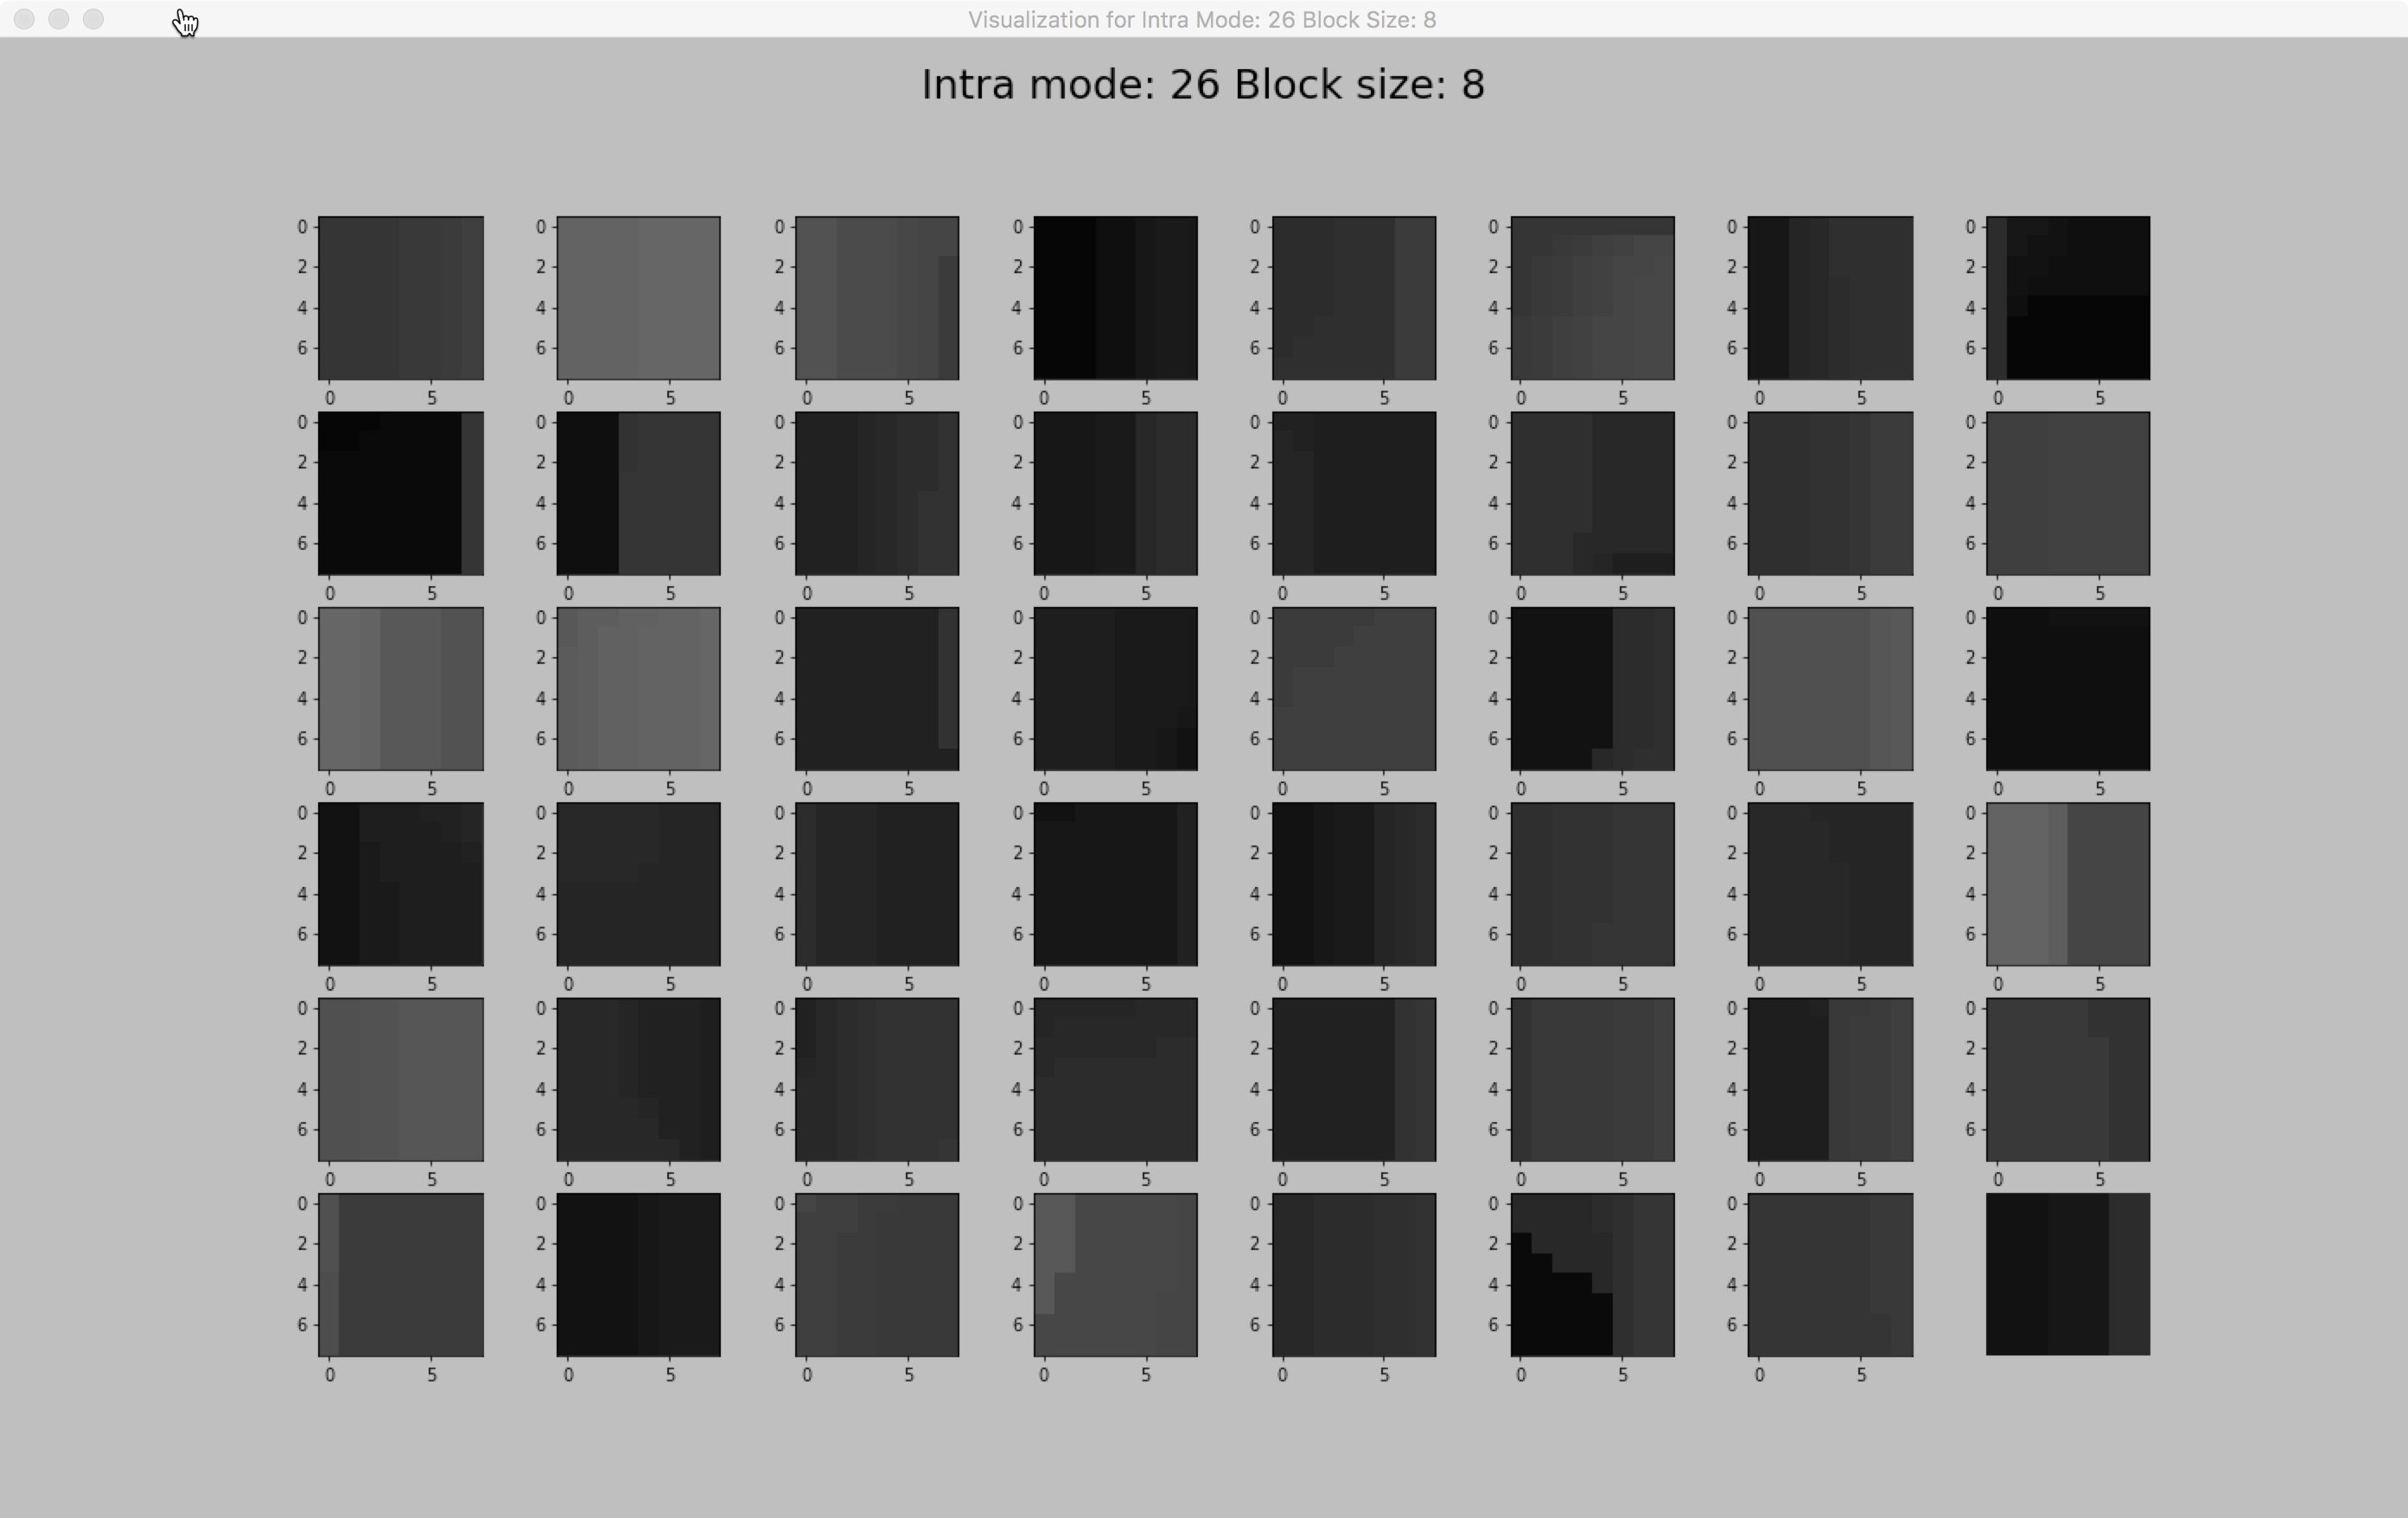
\includegraphics[width=\linewidth]{Figures/visu-size8x8/8-26}
            \caption[Visualizations for blocks tagged with intra mode 26]{Visualizations for blocks tagged with intra mode 26.}
            \label{fig:size8_mode26}
        \end{minipage}
        \hspace{\fill} % note: no blank line here
        \begin{minipage}{0.49\textwidth}
            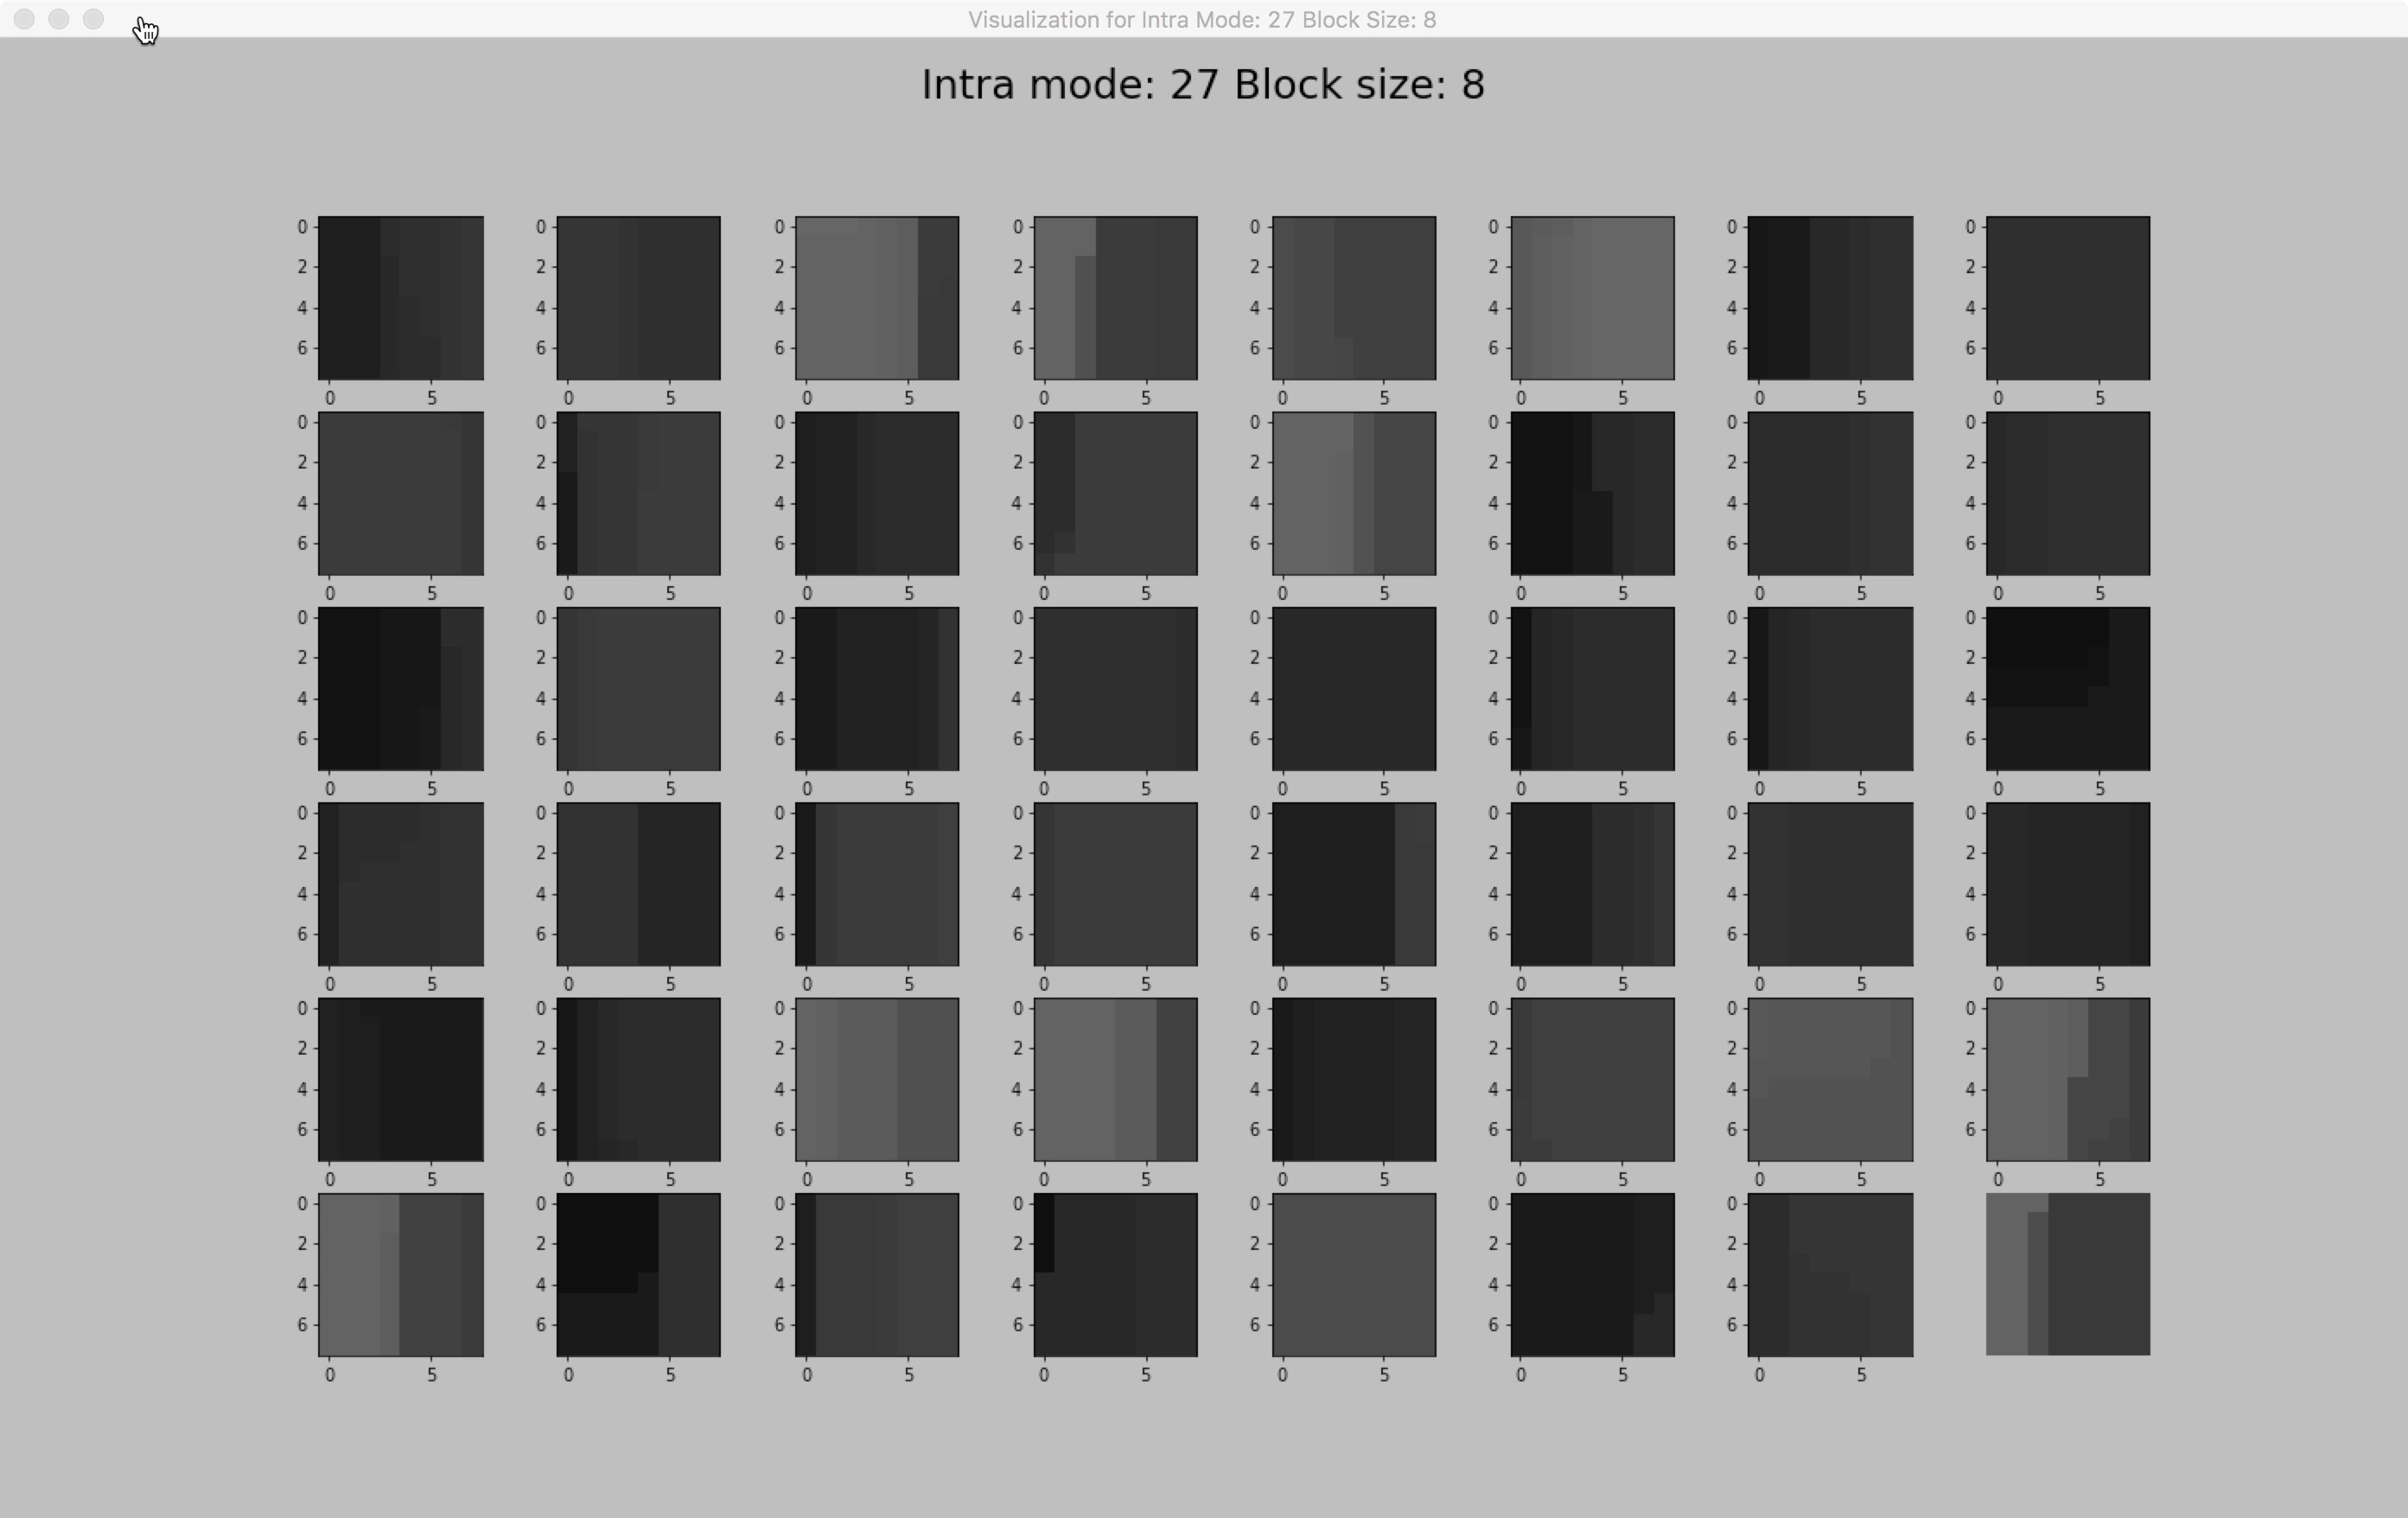
\includegraphics[width=\linewidth]{Figures/visu-size8x8/8-27}
            \caption[Visualizations for blocks tagged with intra mode 27]{Visualizations for blocks tagged with intra mode 27.}
            \label{fig:size8_mode27}
        \end{minipage}
        % \caption{Figure caption goes here}\label{fig:see-data-visu}
    \end{figure}
    
    \begin{figure}
    
        \vspace*{1cm} % vertical separation
    
        \begin{minipage}{0.49\textwidth}
            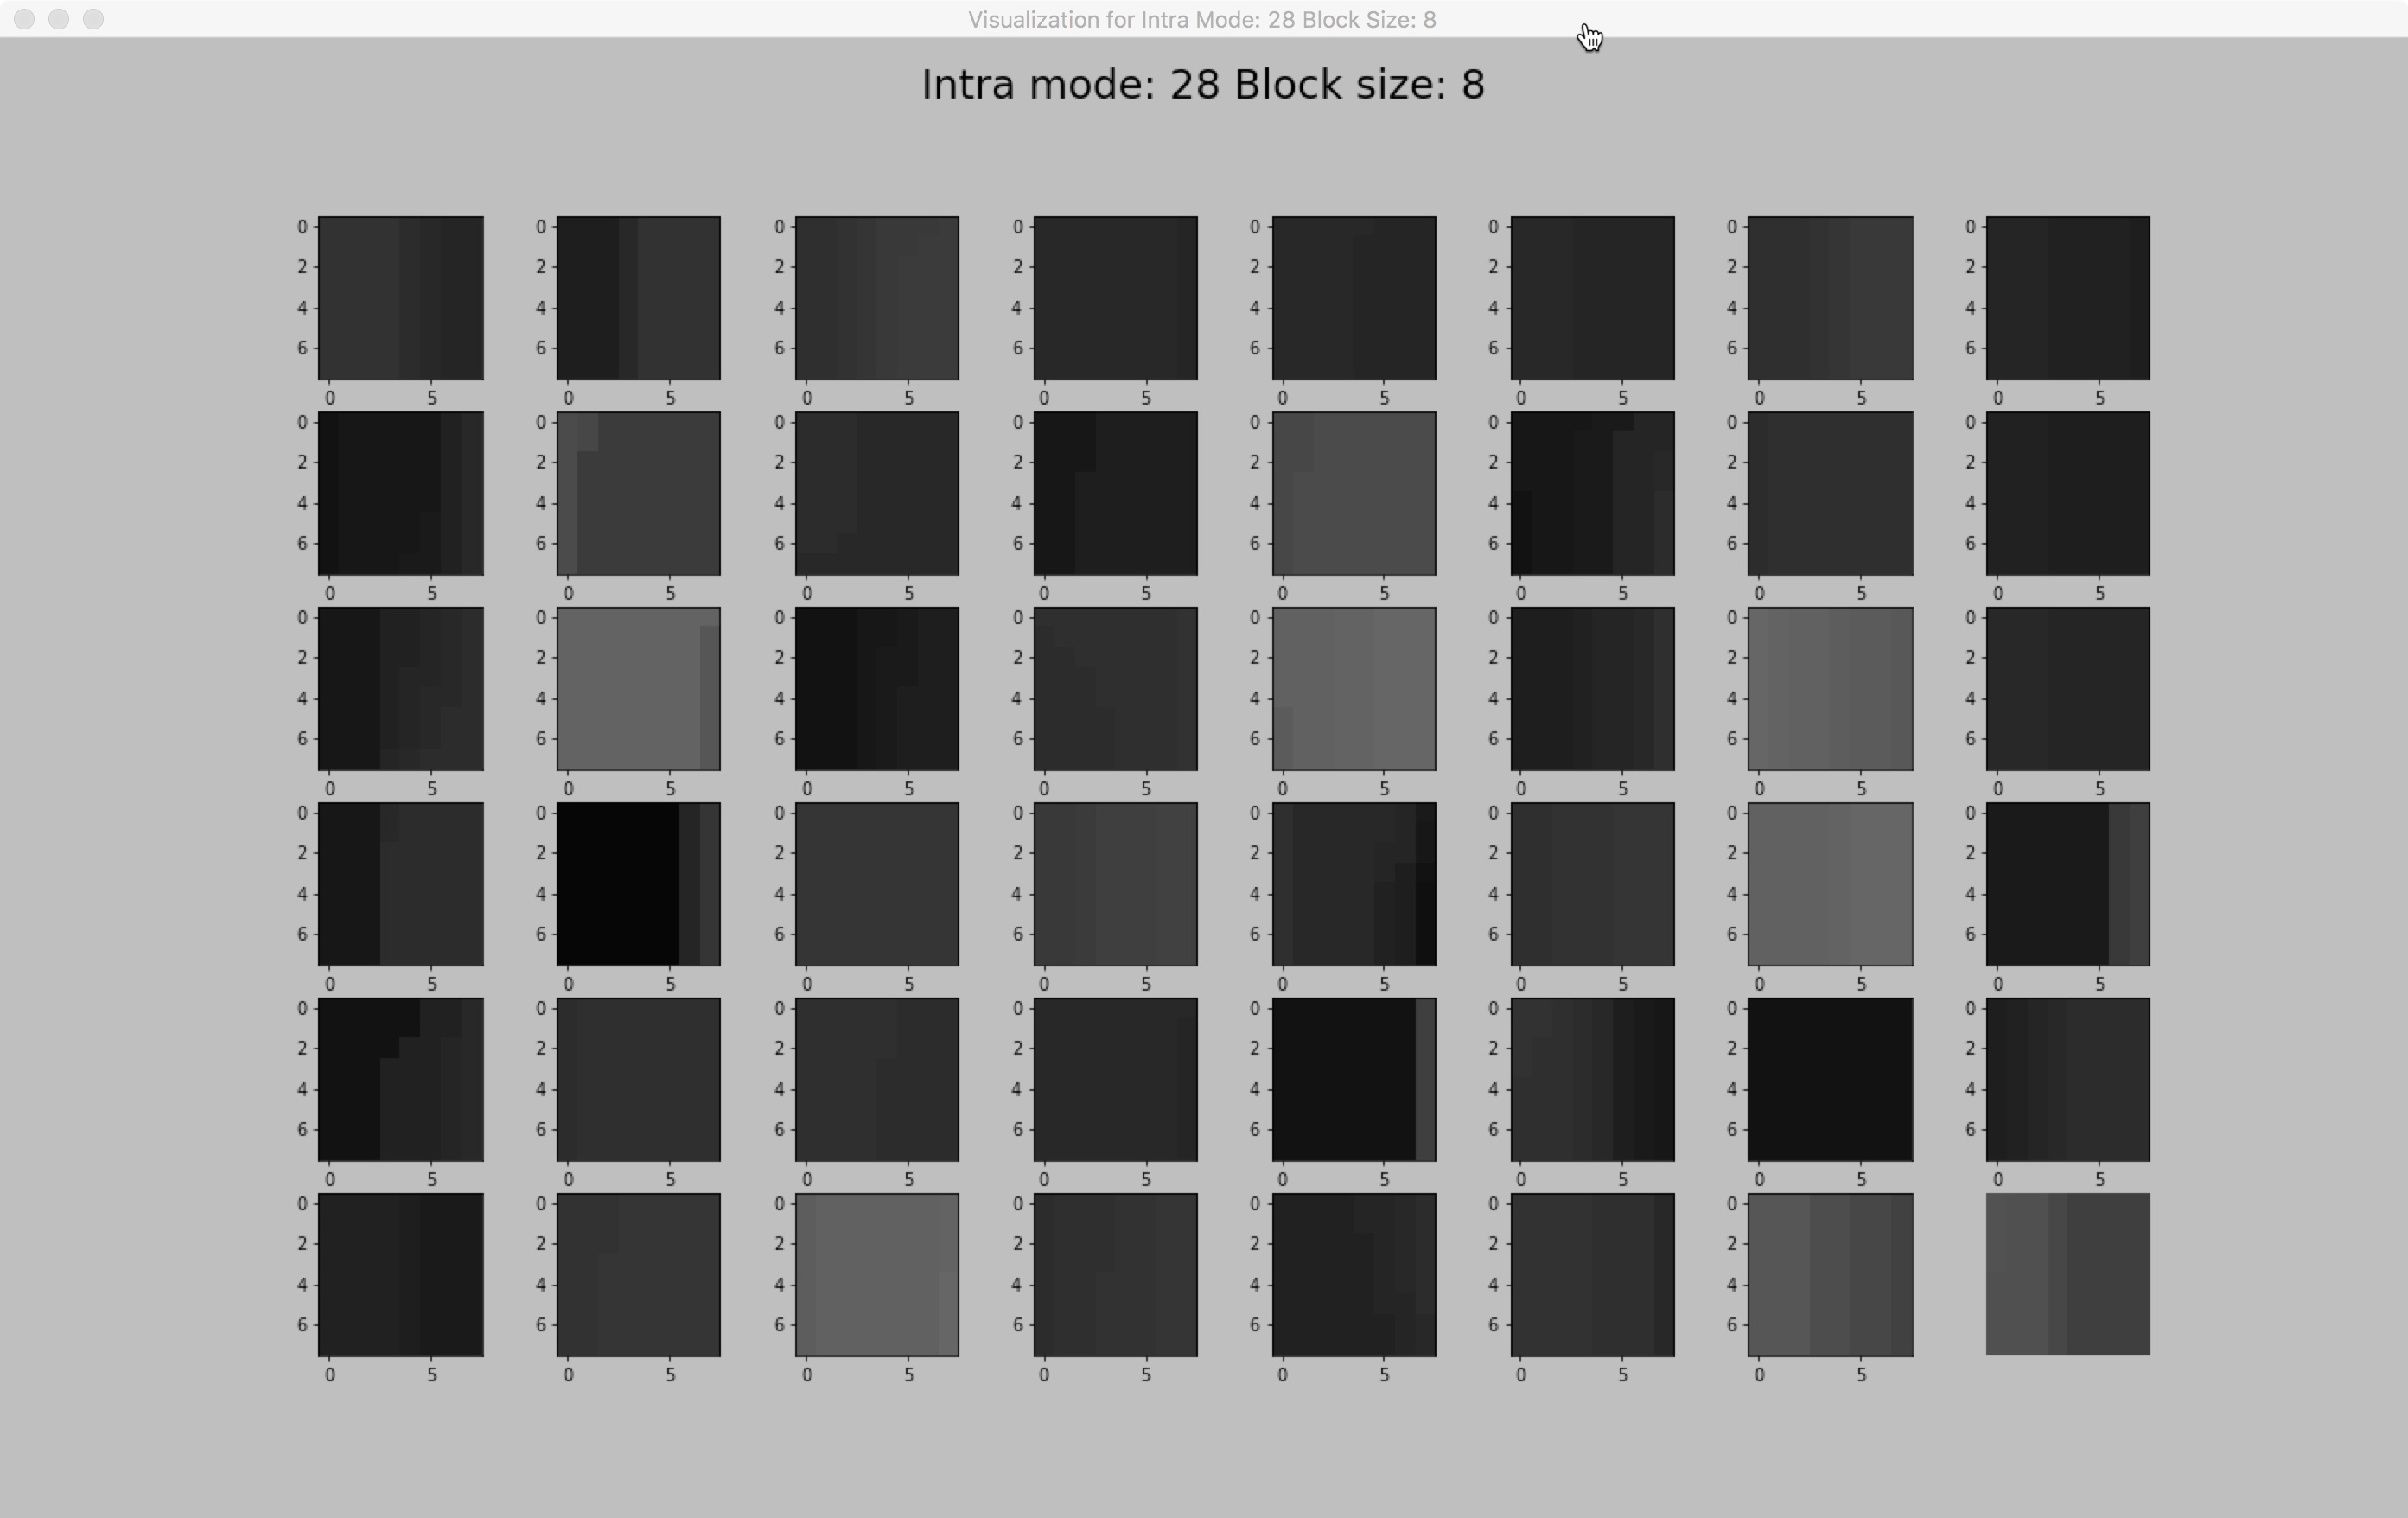
\includegraphics[width=\linewidth]{Figures/visu-size8x8/8-28}
            \caption[Visualizations for blocks tagged with intra mode 28]{Visualizations for blocks tagged with intra mode 28.}
            \label{fig:size8_mode28}
        \end{minipage}
        \hspace{\fill} % note: no blank line here
        \begin{minipage}{0.49\textwidth}
            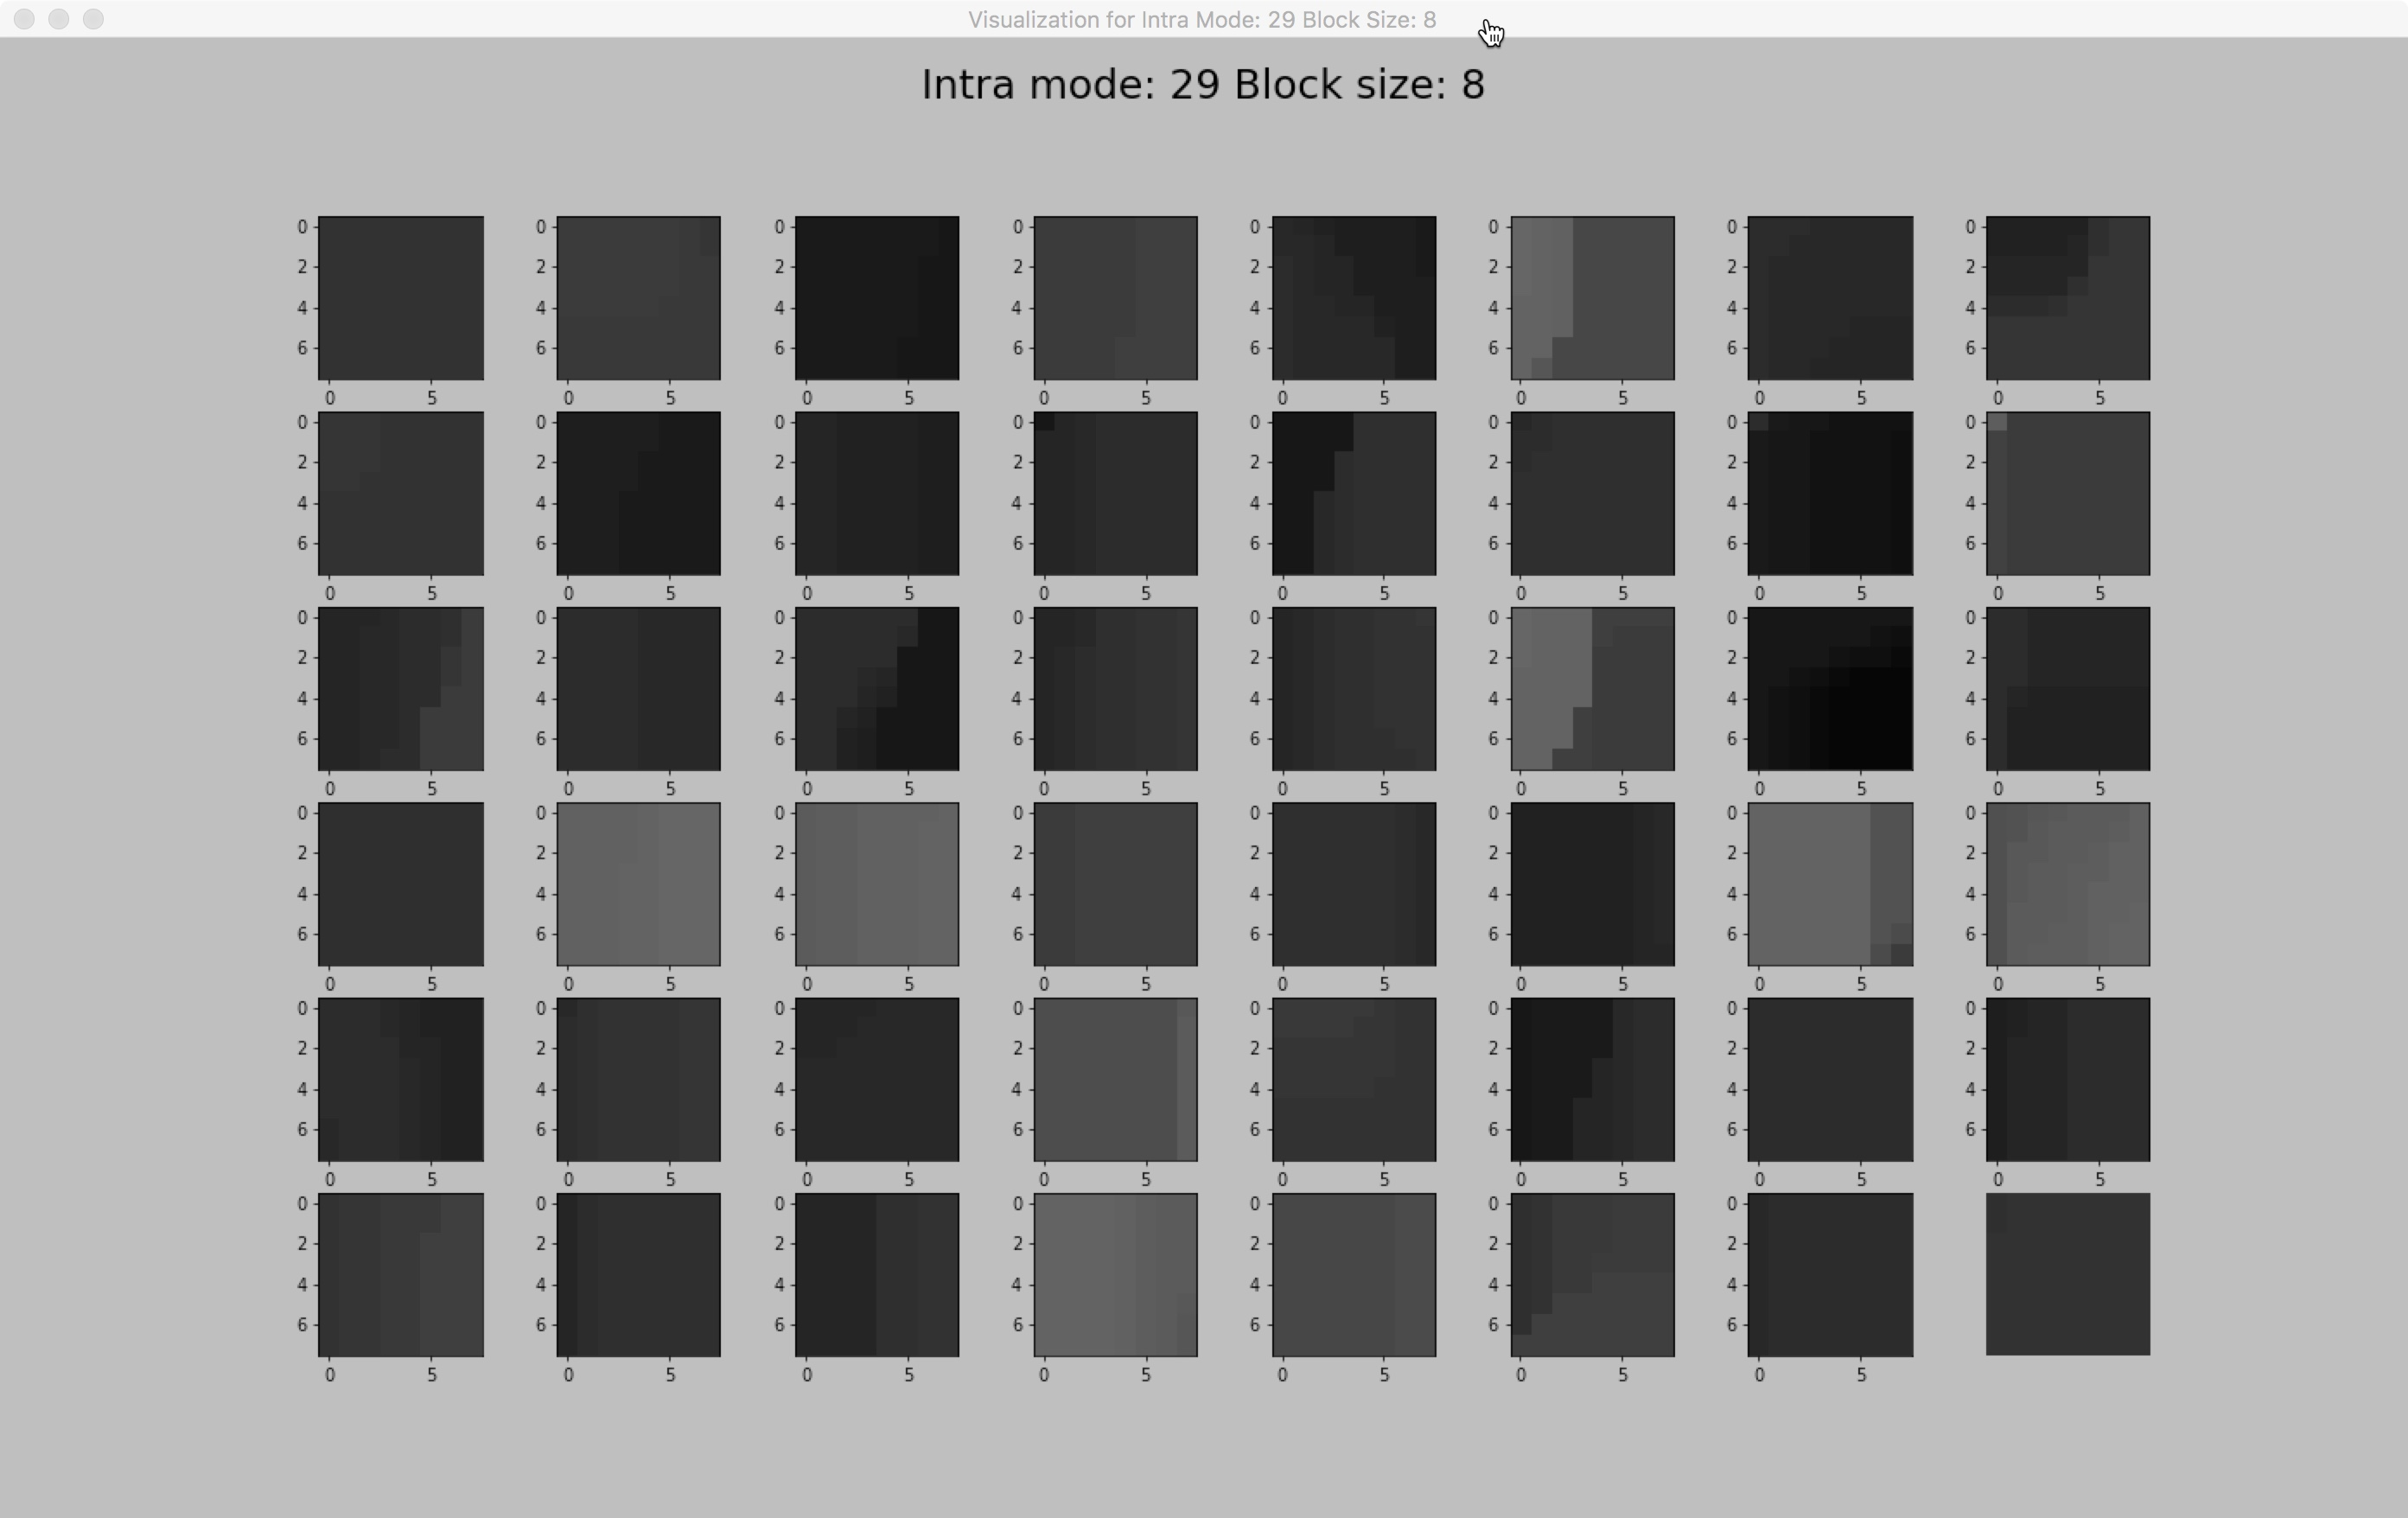
\includegraphics[width=\linewidth]{Figures/visu-size8x8/8-29}
            \caption[Visualizations for blocks tagged with intra mode 29]{Visualizations for blocks tagged with intra mode 29.}
            \label{fig:size8_mode29}
        \end{minipage}
    
        \vspace*{1cm} % vertical separation
    
        \begin{minipage}{0.49\textwidth}
            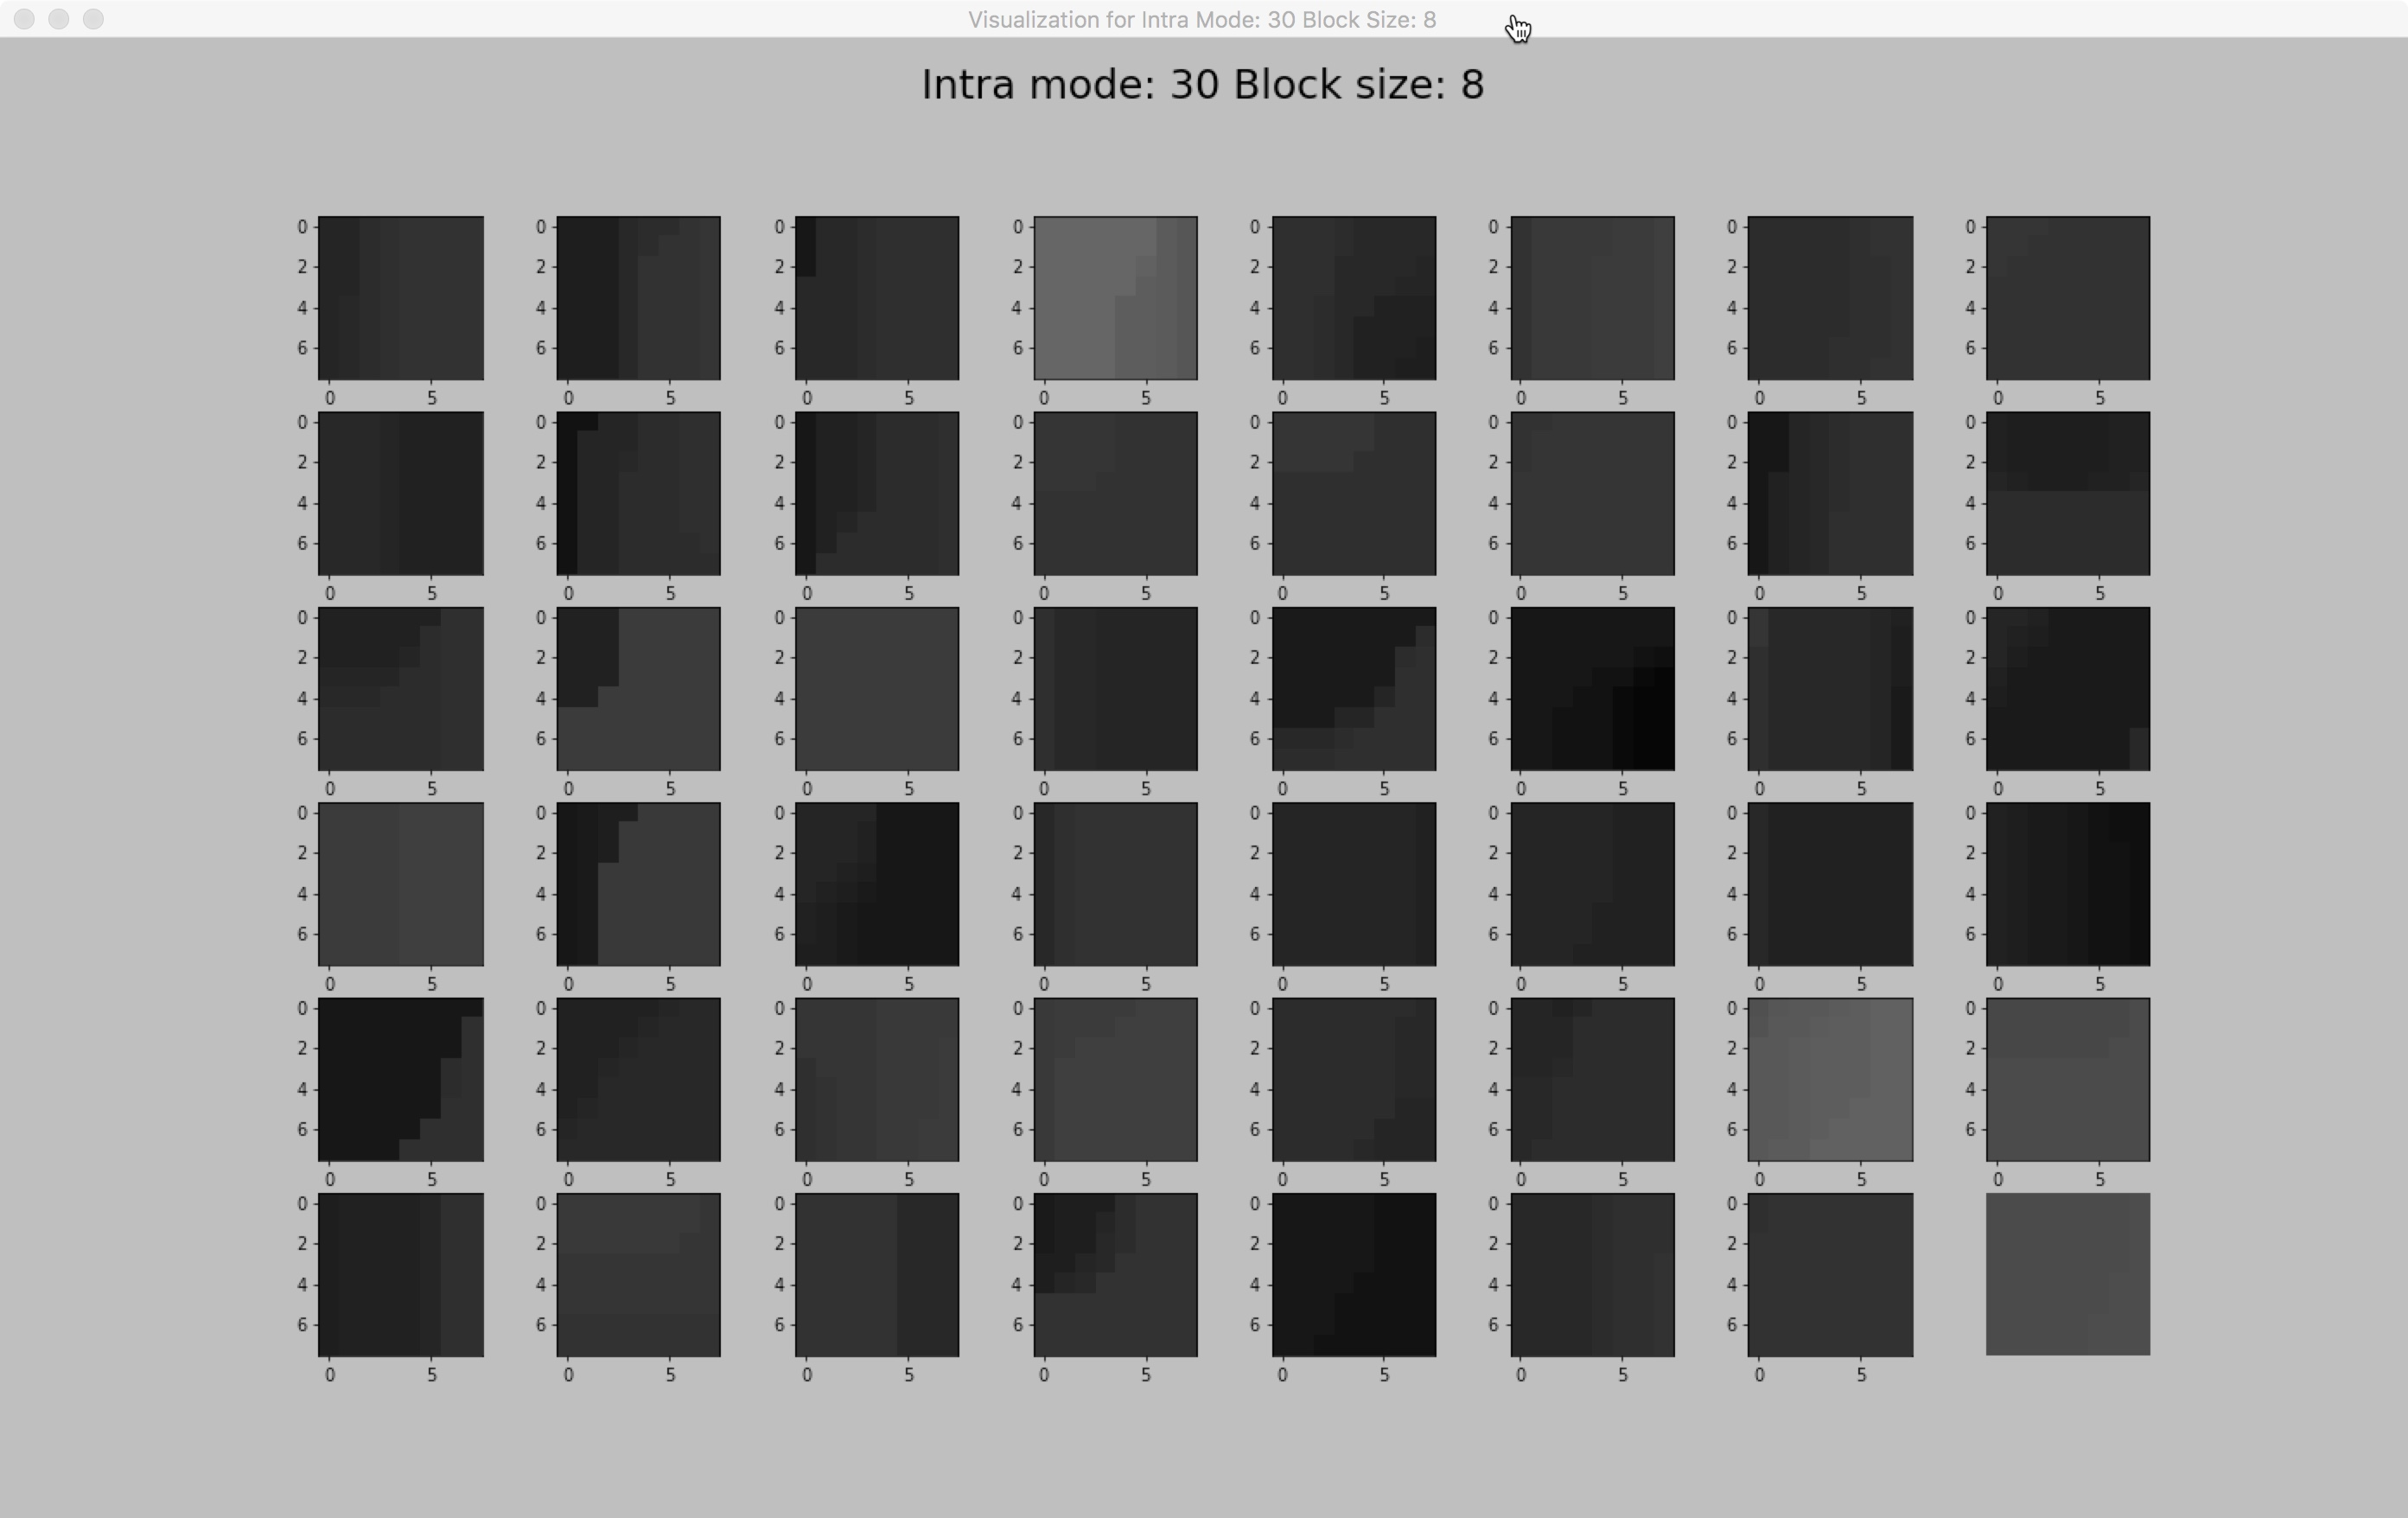
\includegraphics[width=\linewidth]{Figures/visu-size8x8/8-30}
            \caption[Visualizations for blocks tagged with intra mode 30]{Visualizations for blocks tagged with intra mode 30.}
            \label{fig:size8_mode30}
        \end{minipage}
        \hspace{\fill} % note: no blank line here
        \begin{minipage}{0.49\textwidth}
            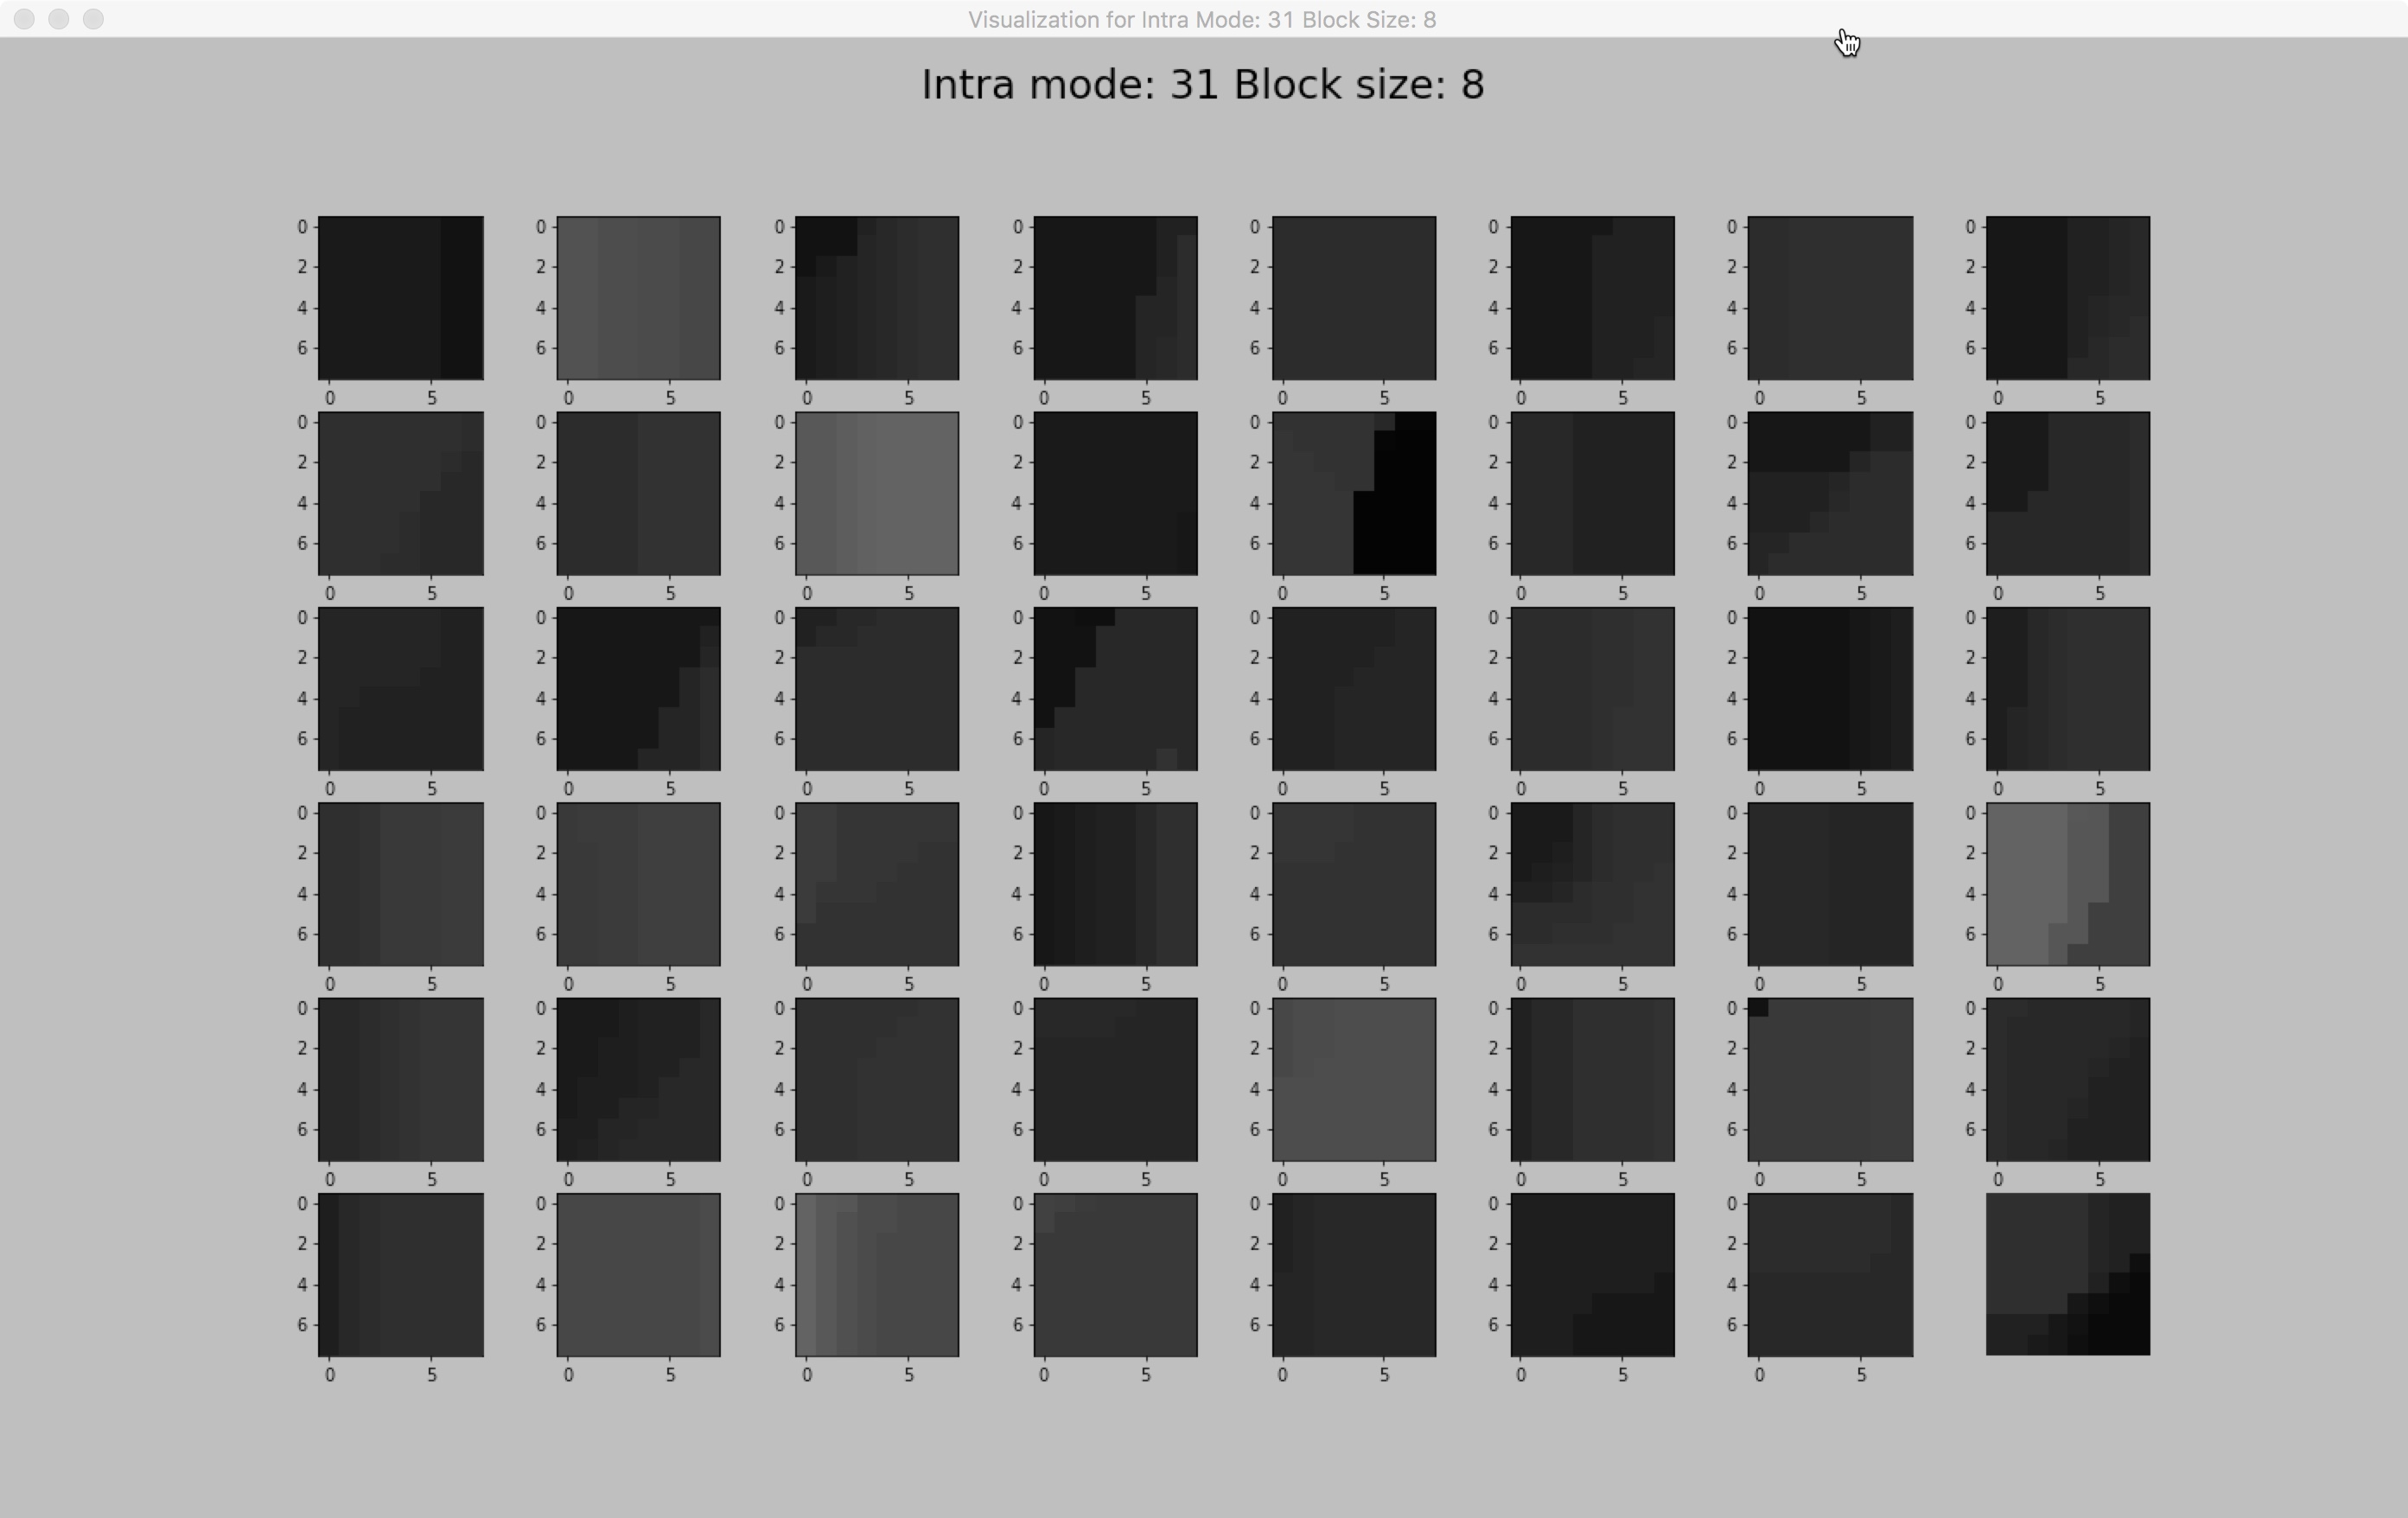
\includegraphics[width=\linewidth]{Figures/visu-size8x8/8-31}
            \caption[Visualizations for blocks tagged with intra mode 31]{Visualizations for blocks tagged with intra mode 31.}
            \label{fig:size8_mode31}
        \end{minipage}
        
        \vspace*{1cm} % vertical separation
    
        \begin{minipage}{0.49\textwidth}
            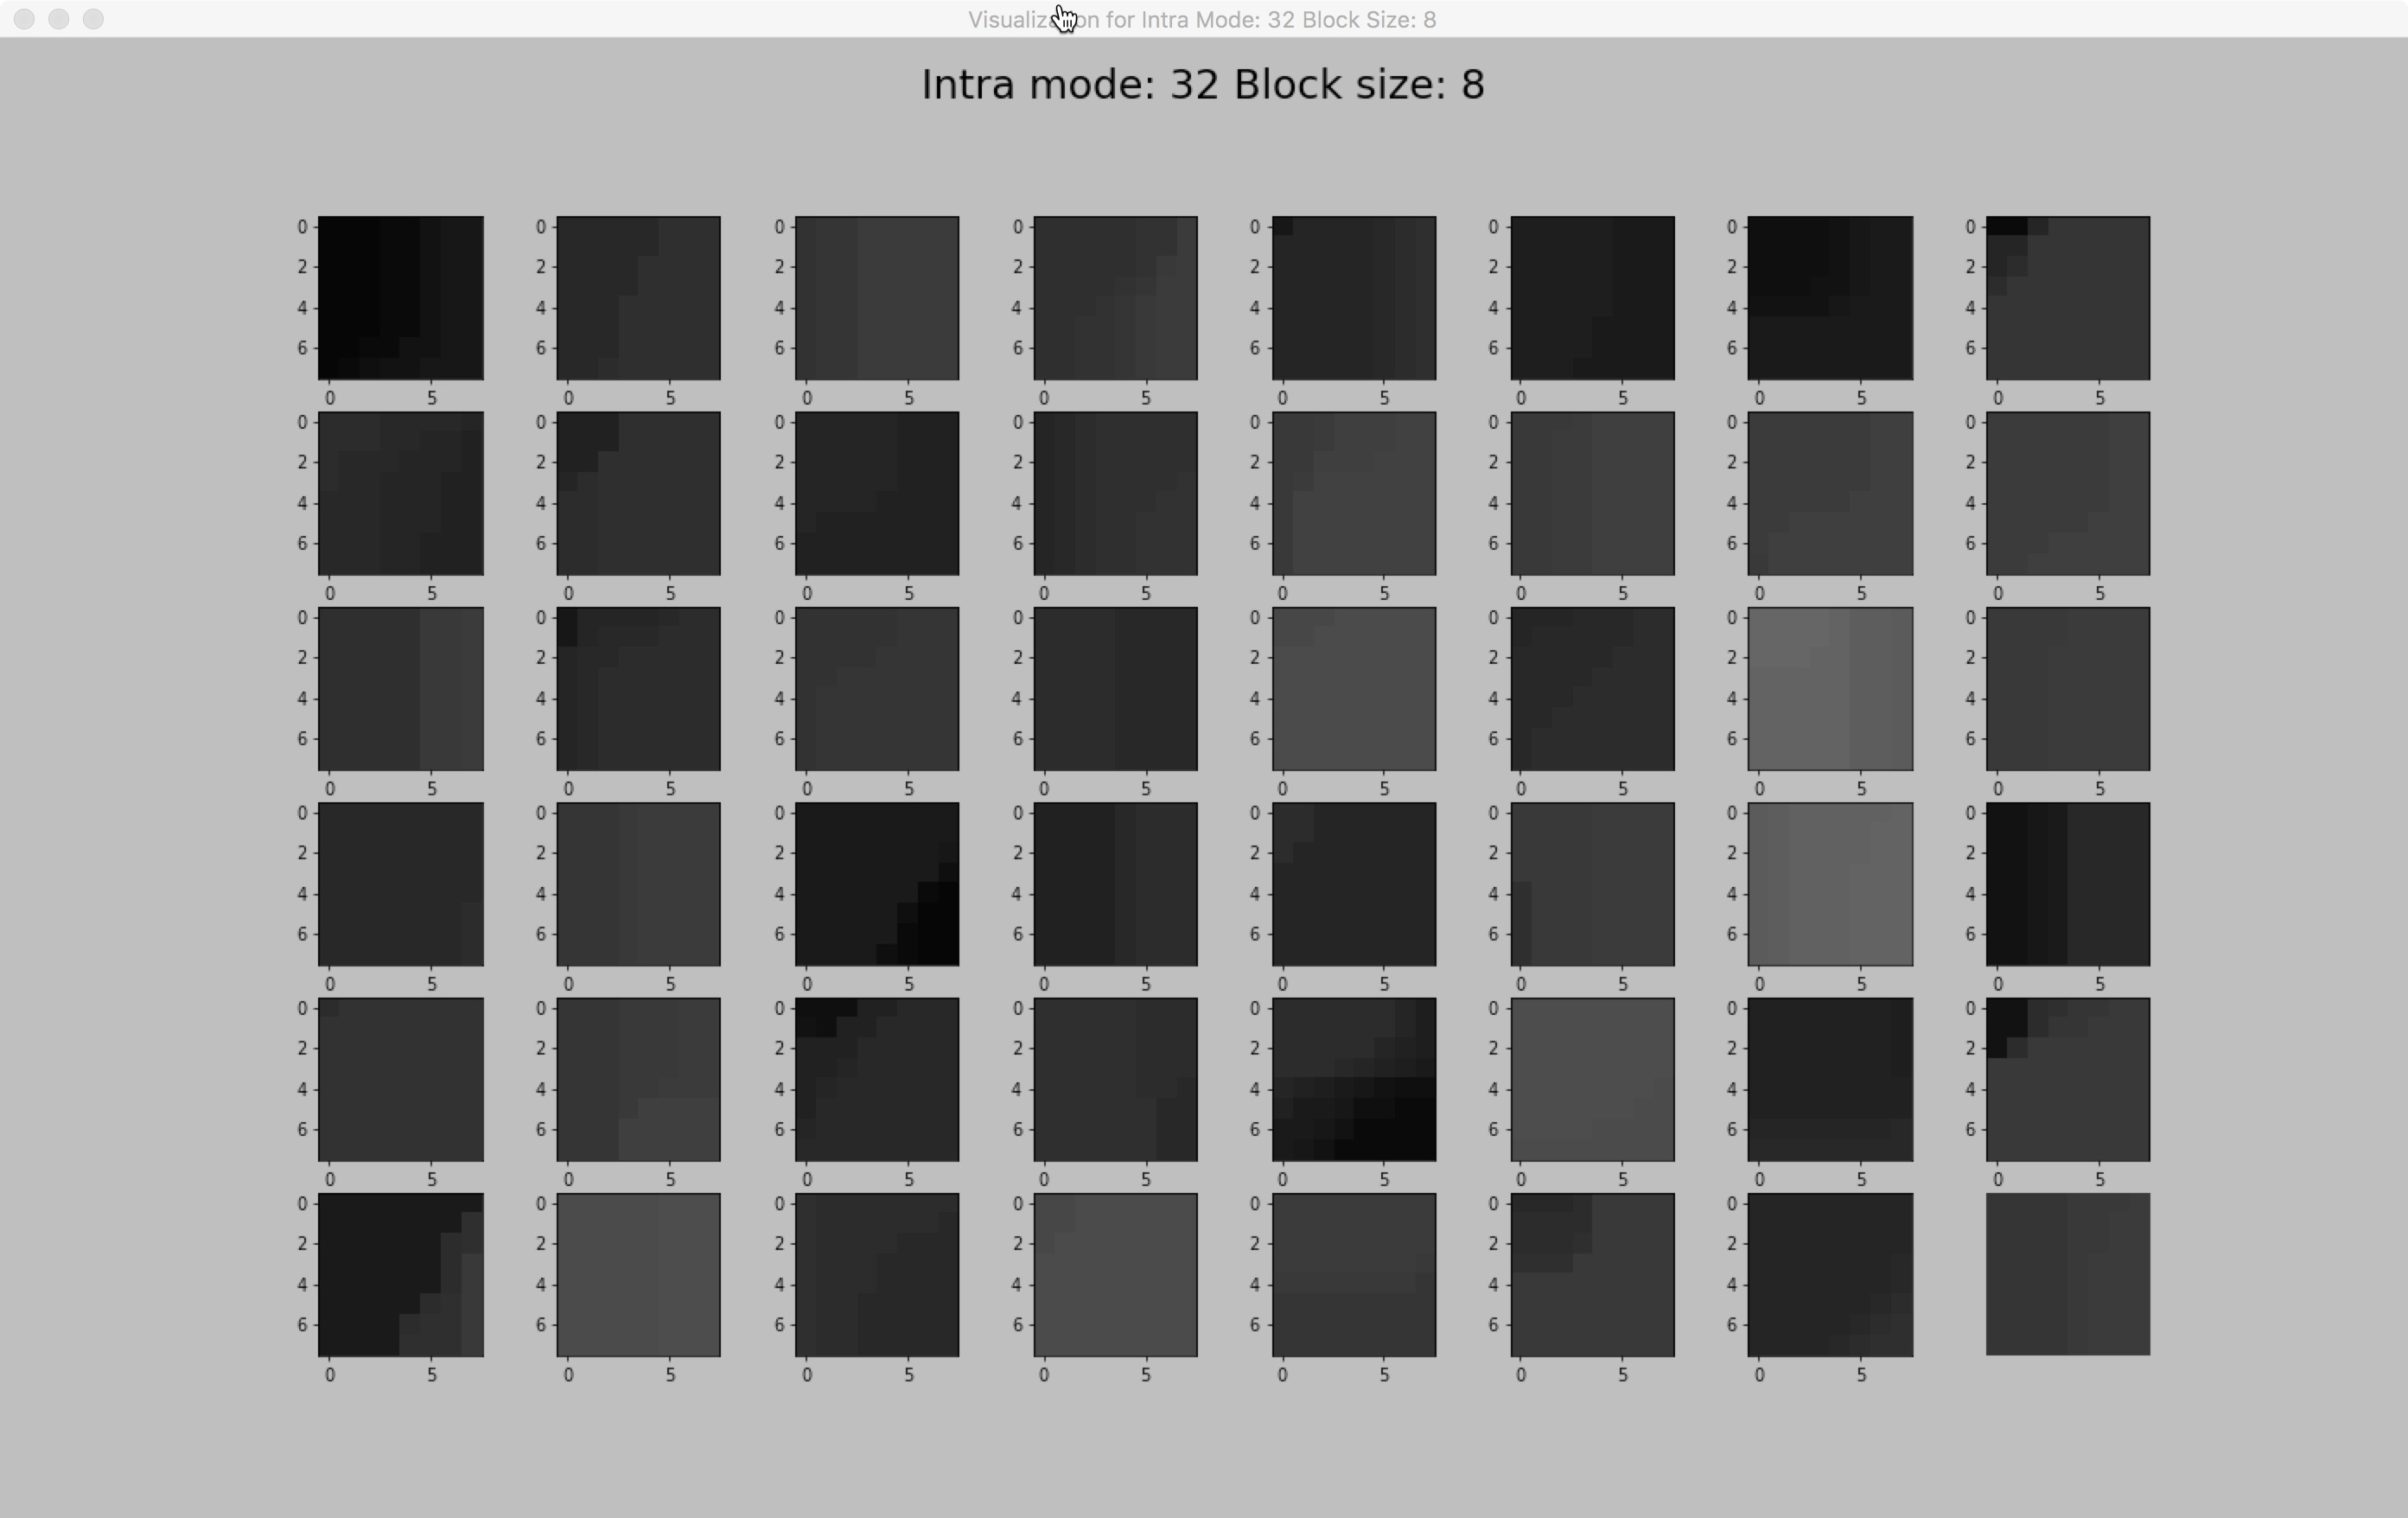
\includegraphics[width=\linewidth]{Figures/visu-size8x8/8-32}
            \caption[Visualizations for blocks tagged with intra mode 32]{Visualizations for blocks tagged with intra mode 32.}
            \label{fig:size8_mode32}
        \end{minipage}
        \hspace{\fill} % note: no blank line here
        \begin{minipage}{0.49\textwidth}
            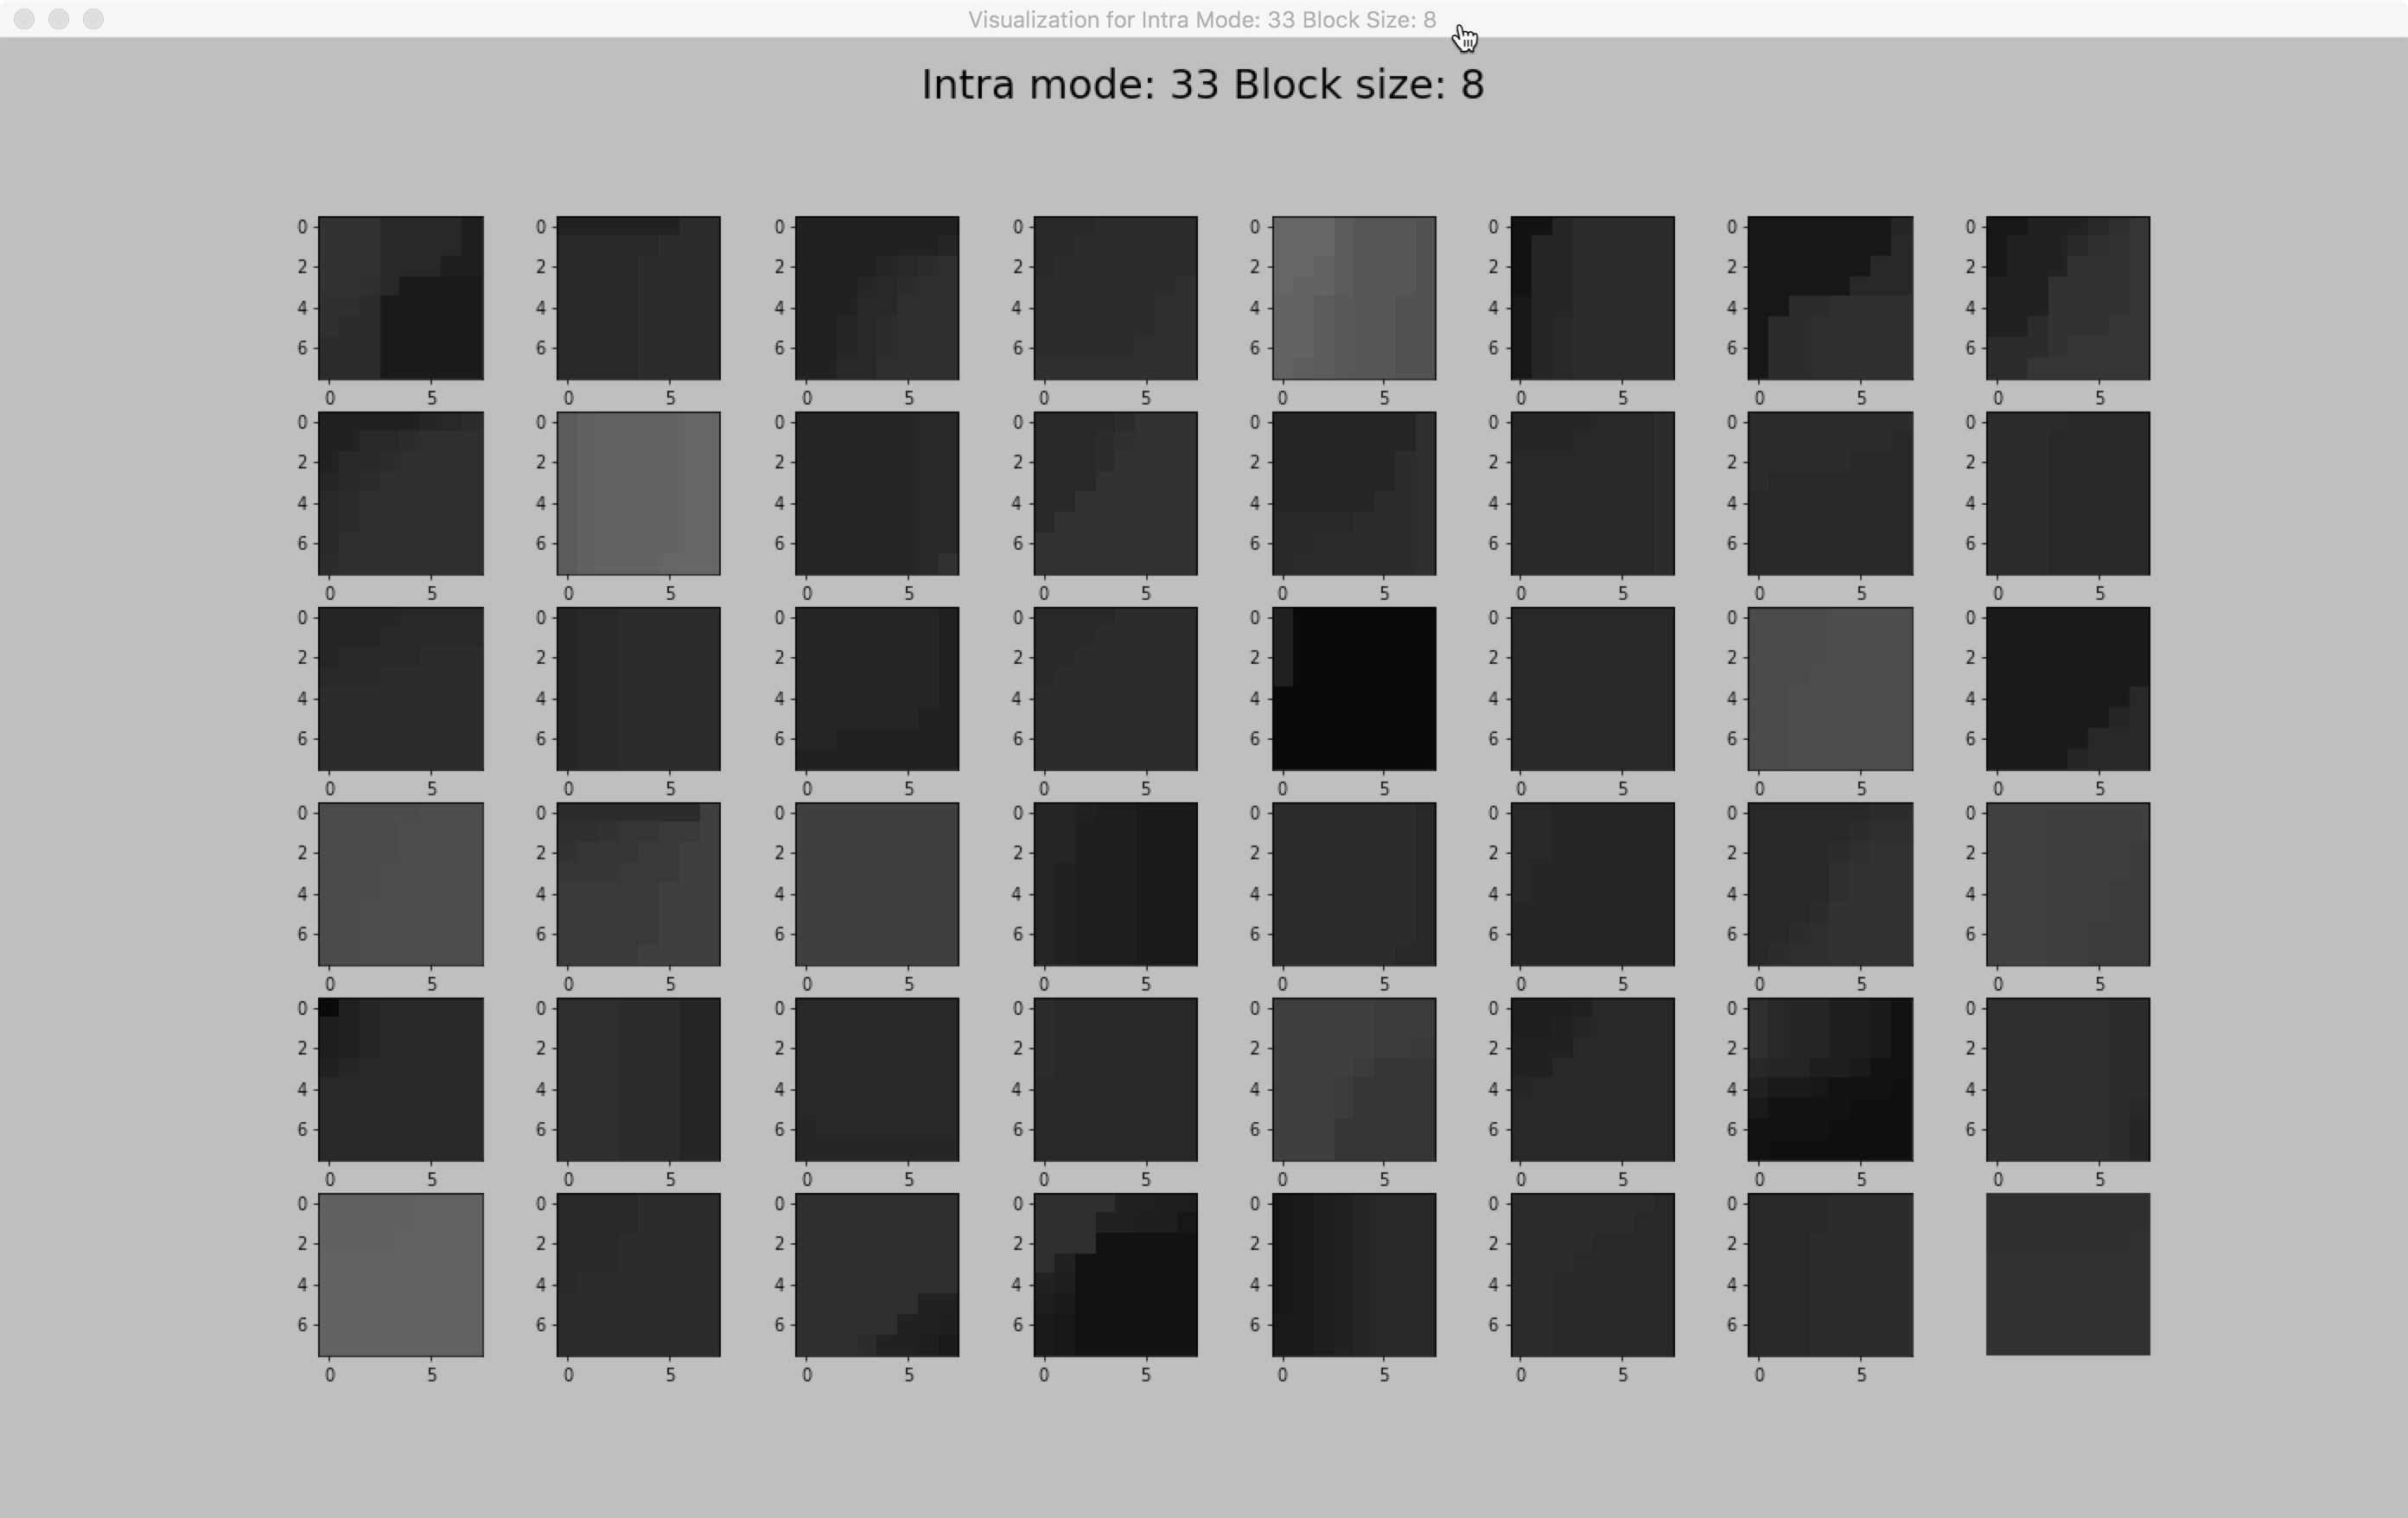
\includegraphics[width=\linewidth]{Figures/visu-size8x8/8-33}
            \caption[Visualizations for blocks tagged with intra mode 33]{Visualizations for blocks tagged with intra mode 33.}
            \label{fig:size8_mode33}
        \end{minipage}
    % \caption{Figure caption goes here}\label{fig:see-data-visu}
    \end{figure}
    \begin{figure}
        \vspace*{1cm} % vertical separation
        \begin{minipage}{0.49\textwidth}
            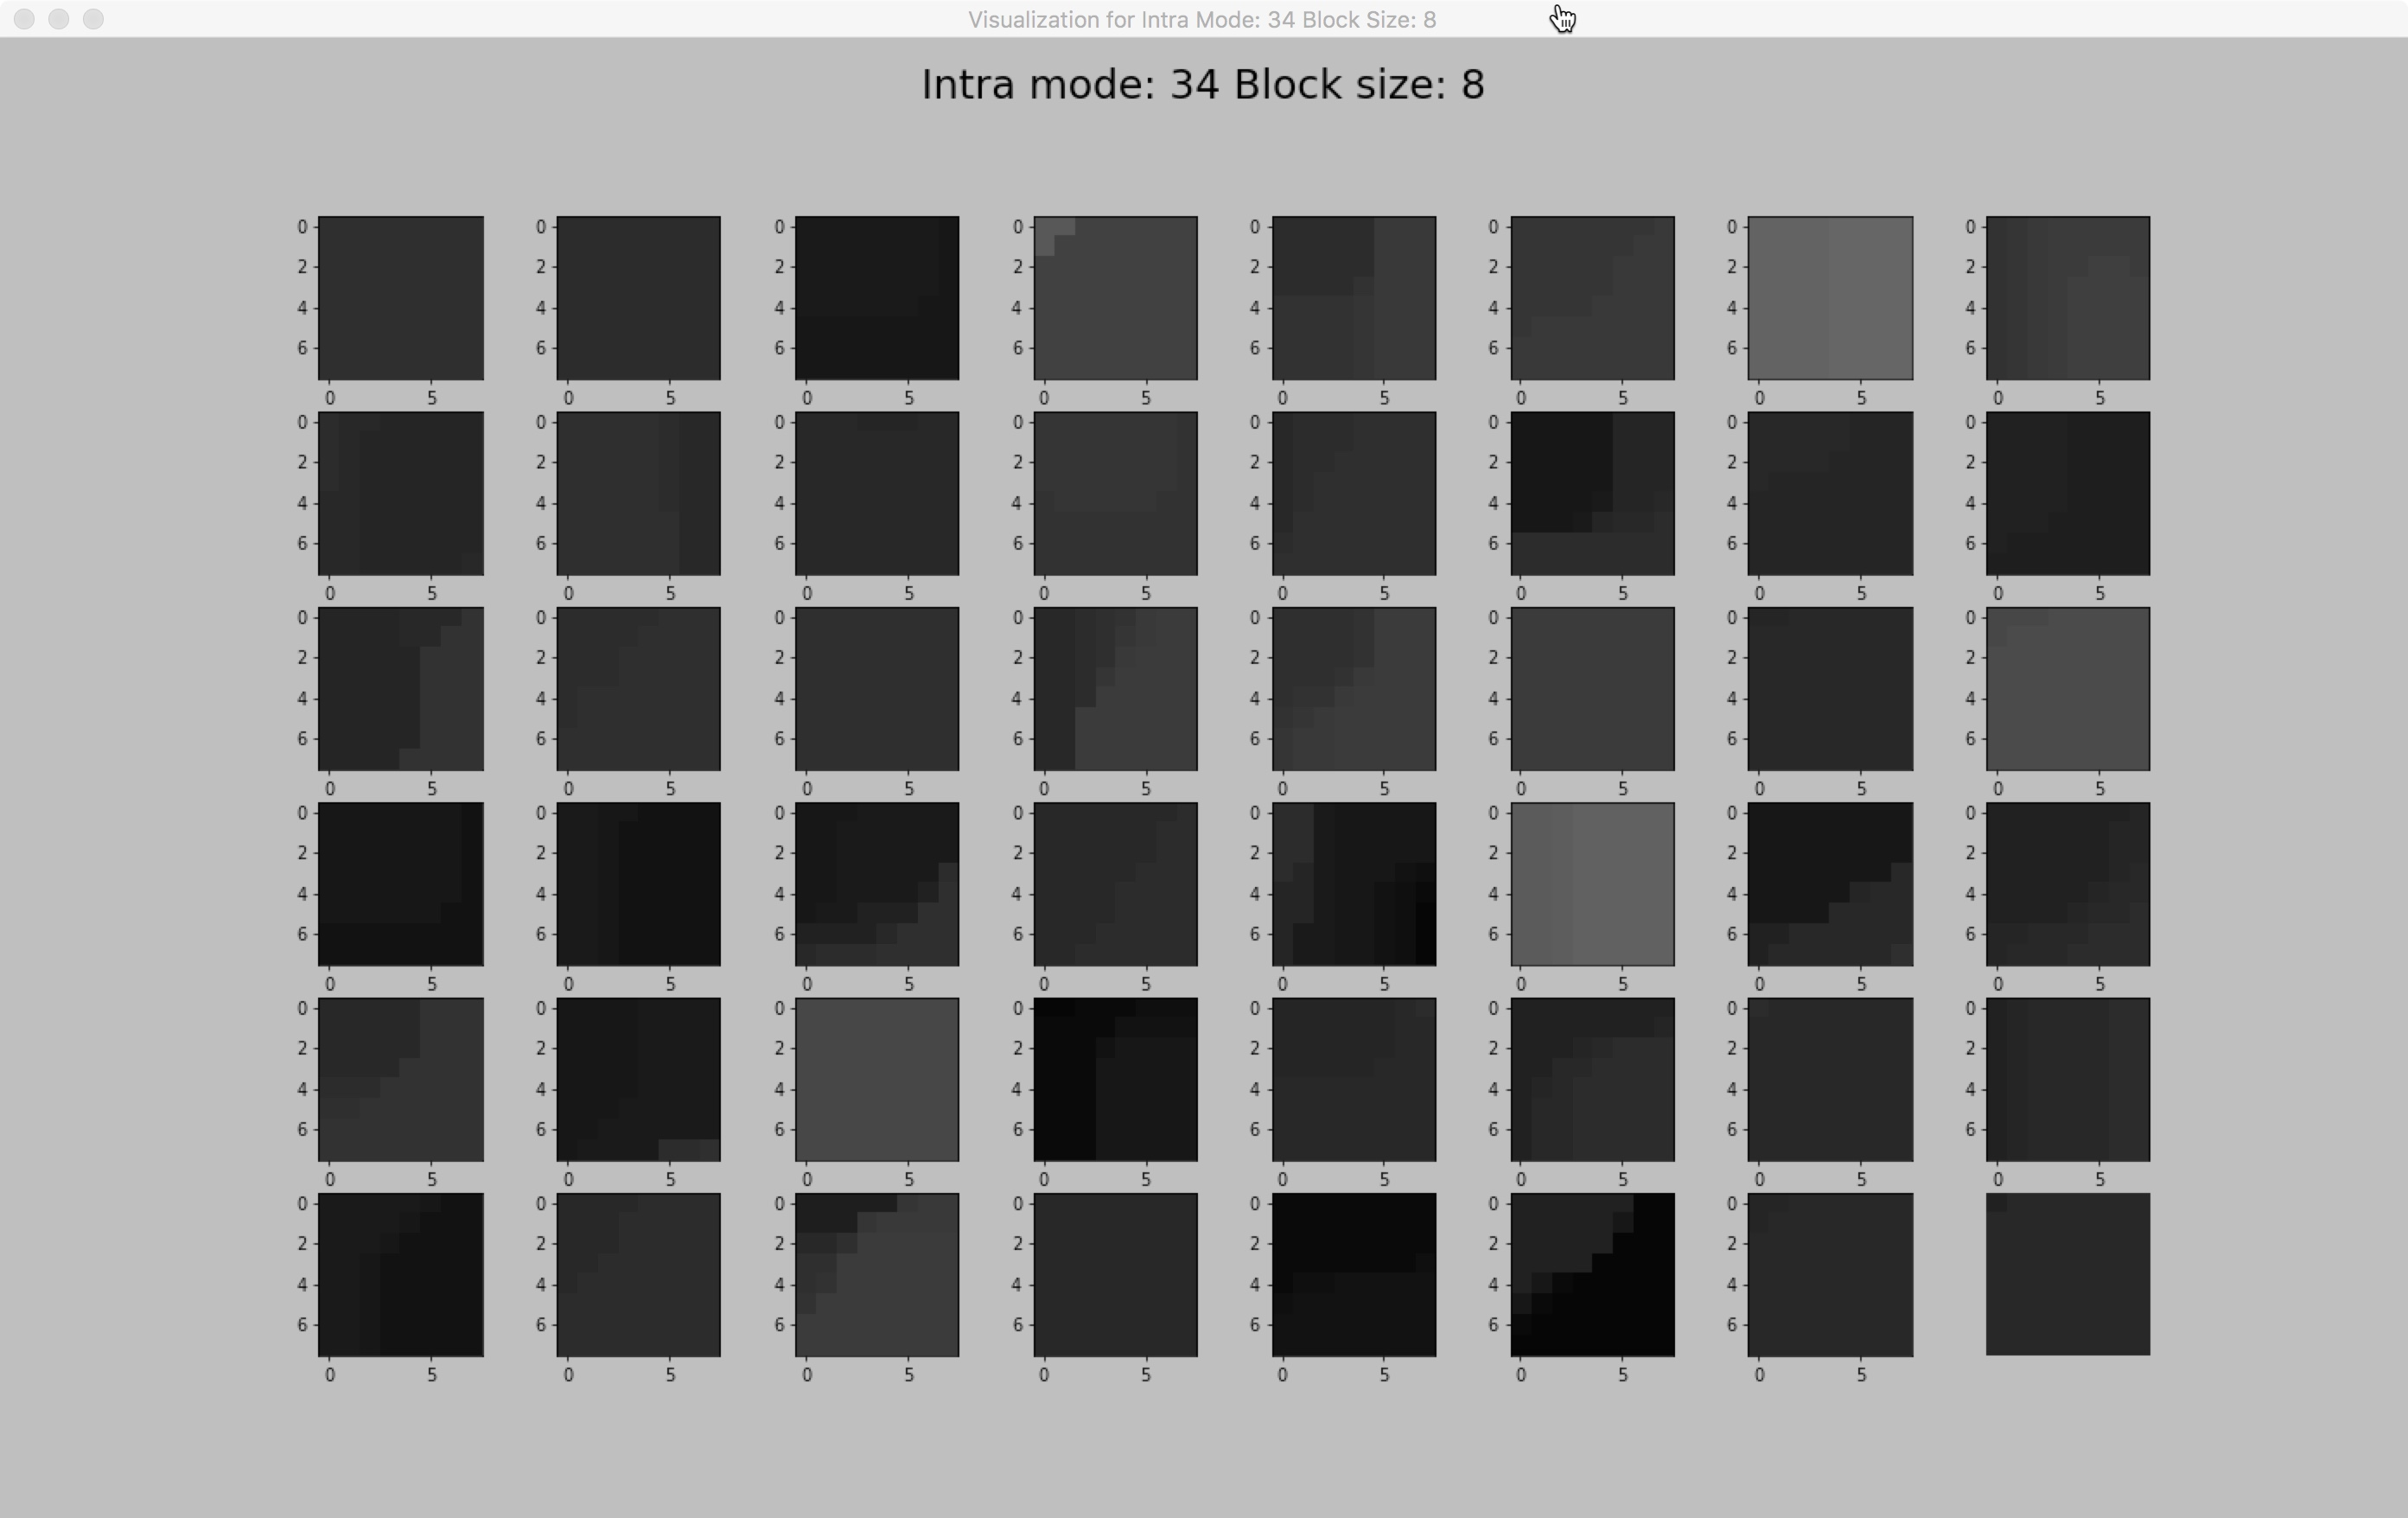
\includegraphics[width=\linewidth]{Figures/visu-size8x8/8-34}
            \caption[Visualizations for blocks tagged with intra mode 34]{Visualizations for blocks tagged with intra mode 34.}
            \label{fig:size8_mode34}
        \end{minipage}
        \hspace{\fill} % note: no blank line here
        \begin{minipage}{0.49\textwidth}
            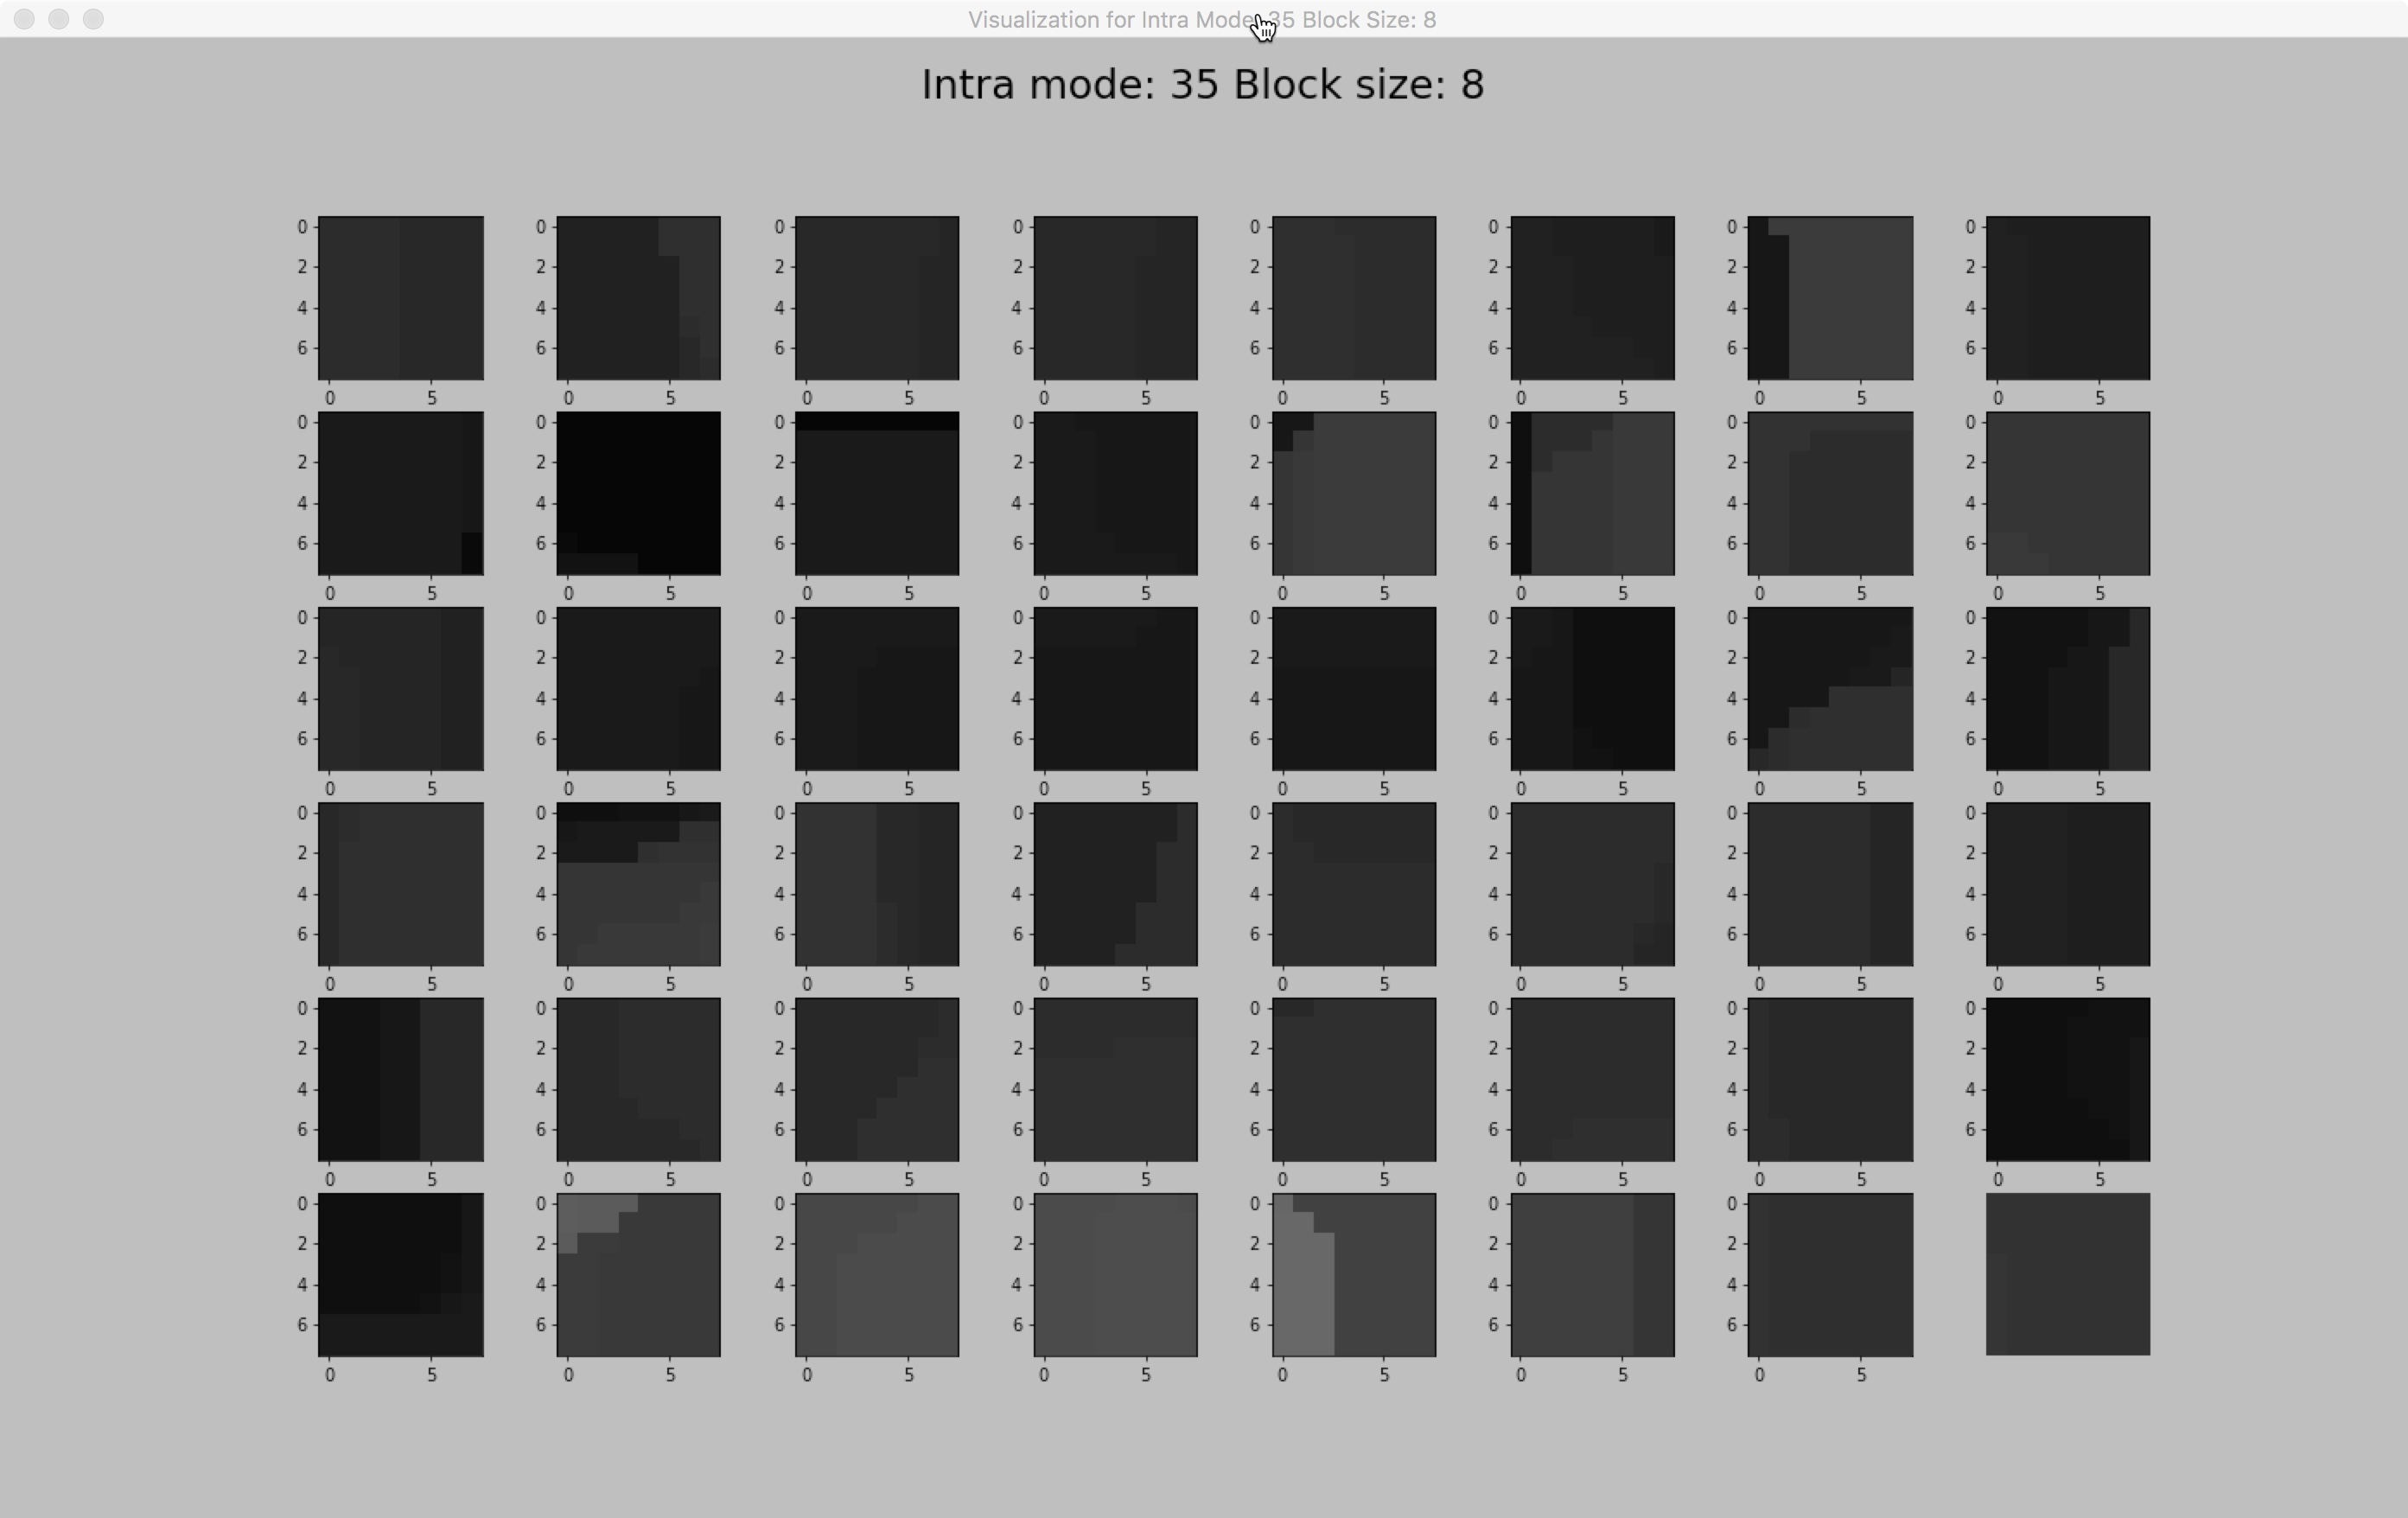
\includegraphics[width=\linewidth]{Figures/visu-size8x8/8-35}
            \caption[Visualizations for blocks tagged with DMM1]{Visualizations for blocks tagged with DMM1}
            \label{fig:size8_mode35}
        \end{minipage}
    
        \vspace*{1cm} % vertical separation
    
        \begin{minipage}{0.49\textwidth}
            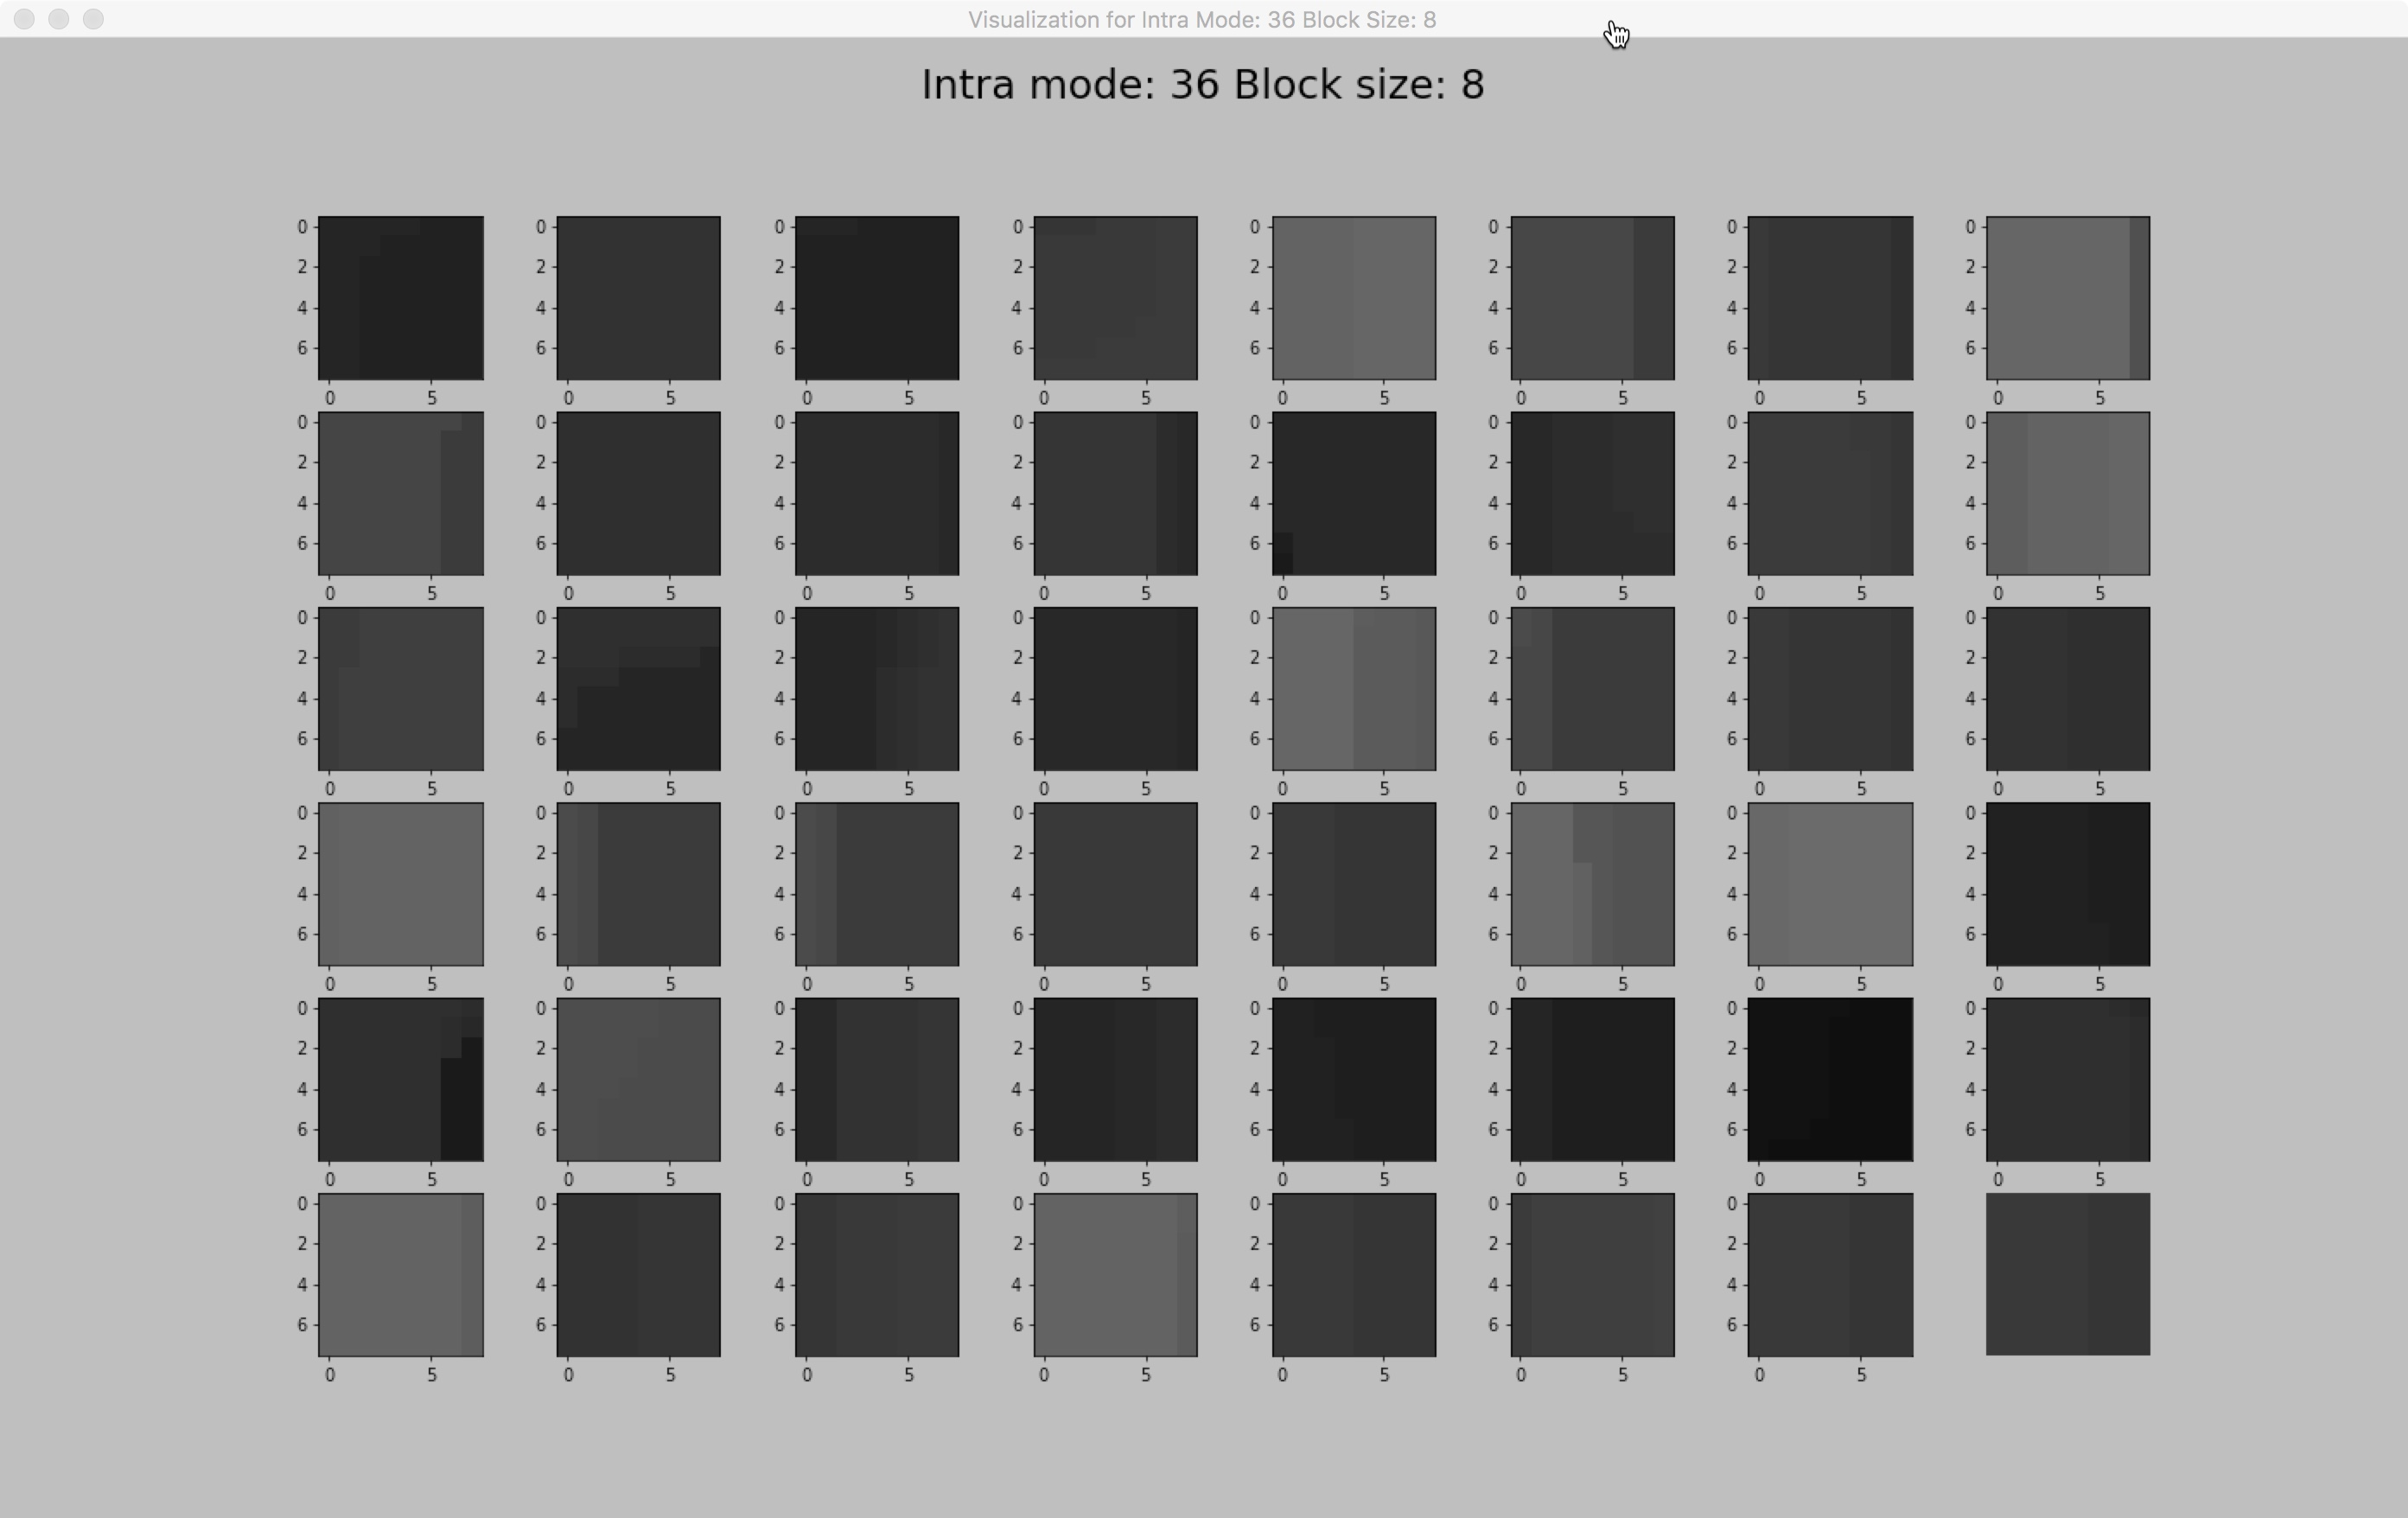
\includegraphics[width=\linewidth]{Figures/visu-size8x8/8-36}
            \caption[Visualizations for blocks tagged with DMM4]{Visualizations for blocks tagged with DMM4}
            \label{fig:size8_mode36}
        \end{minipage}
        % \caption{Figure caption goes here}\label{fig:see-data-visu}
    \end{figure}

\subsection{Discussion}\label{subsec:discussion-about-data-visu}
From the visualizations of blocks of size \(8\times8\),
it is found that within blocks of each single angular mode,
part of them have sharp edges that can 
be easily perceived by human while the others 
are very smooth such that their edges can not be clearly seem
unless they are enlarged by multiple times.
When blocks with such a mixed style are fed into the 
convolutional neural networks, the prediction accuracy
is always not ideal enough to be used
inside the reference software of 3D-HEVC\@.
However, the same model learns well on other 
benchmark datasets such as 
MNIST~\parencite{XRN001} and CIFAR~\parencite{XRN002}.
There are two explanations to this phenomenon.
One is that the mix of extreme smoothness and
clear sharpness inside blocks of each single 
intra prediction mode
yields impure datasets such that the neural networks
are not able to figure out the intrinsic abstractions
layer by layer.
The other is that our network size is not deep enough
to have the capability of learning representations 
for such a mixed style. 
Meanwhile, the size of 
the dataset cannot satisfy large networks
due to the limited information in the 
training dataset.
The size of collected data is not abundant such that
there is no chance of feeding a large dataset
to the computational model for the time being.
Moreover, larger neural networks require more 
computational power which can be very expensive.
Combining the two considerations above, 
eliminating extreme smoothness is the way to go,
by which the blocks with vague edges are removed
from datasets.

Mode DC, PLANAR, DMM1 and DMM4 need special attention.
For DC and PLANAR, since most of their blocks
have weak edges with patterns that look
very similar to angular modes,
intuitively it seems not practical to require 
neural network to learn to 
distinguish them from angular modes.
For DMM1 which is particularly designed for depth maps,
it is noticed that lots of their
blocks contain straight edges with arbitrary positions.
Hence the learned model may predict DMM1 into any
of the 33 angular modes according to the angle of
the partition line in DMM1 blocks.
DMM4 is another dedicated mode for depth maps.
Most of their blocks feature contour partitions instead of
straight lines.
Some contours nevertheless cannot show 
their clear characteristics that can 
discriminate themselves
from angular modes which have some curvilinear distortions.

In fact, according to our experiments,
the deep neural network, which has 
an architecture that works well on 
benchmark datasets, does not work well on 
the collected dataset comprising modes
[DC, PLANAR, 2, \ldots, 34, DMM1, DMM4].
During the training process, the validations
are performed in a regular frequency to monitor 
the performance of the learned model.
\begin{figure}
    \begin{minipage}{0.49\textwidth}
        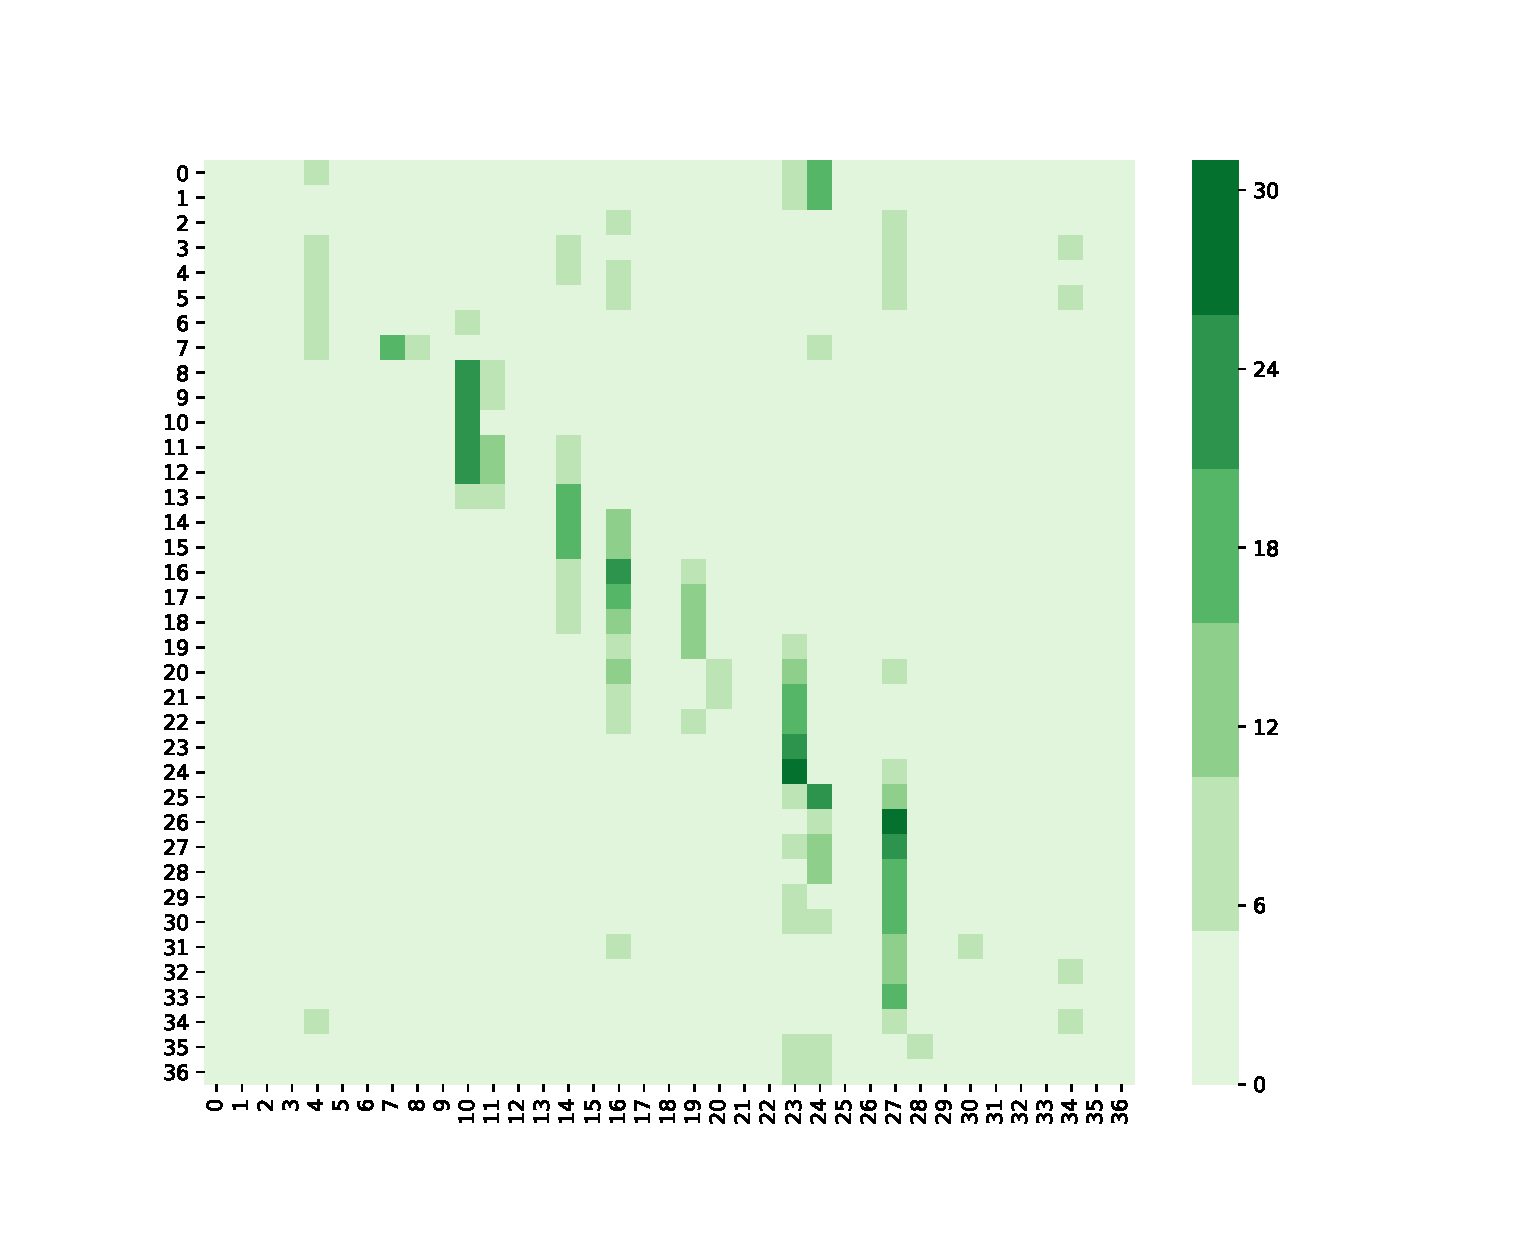
\includegraphics[width=\textwidth,height=\textheight,keepaspectratio]{Figures/confusion-matrix/ckpt-10342.eps}
        \caption[Confusion matrix obtained after 12 epochs of model training]
        {Confusion matrix obtained after 12 epochs of model training}
        \label{fig:cm-after-12-epochs}
    \end{minipage}
    \hspace{\fill} % note: no blank line here
    \begin{minipage}{0.49\textwidth}
        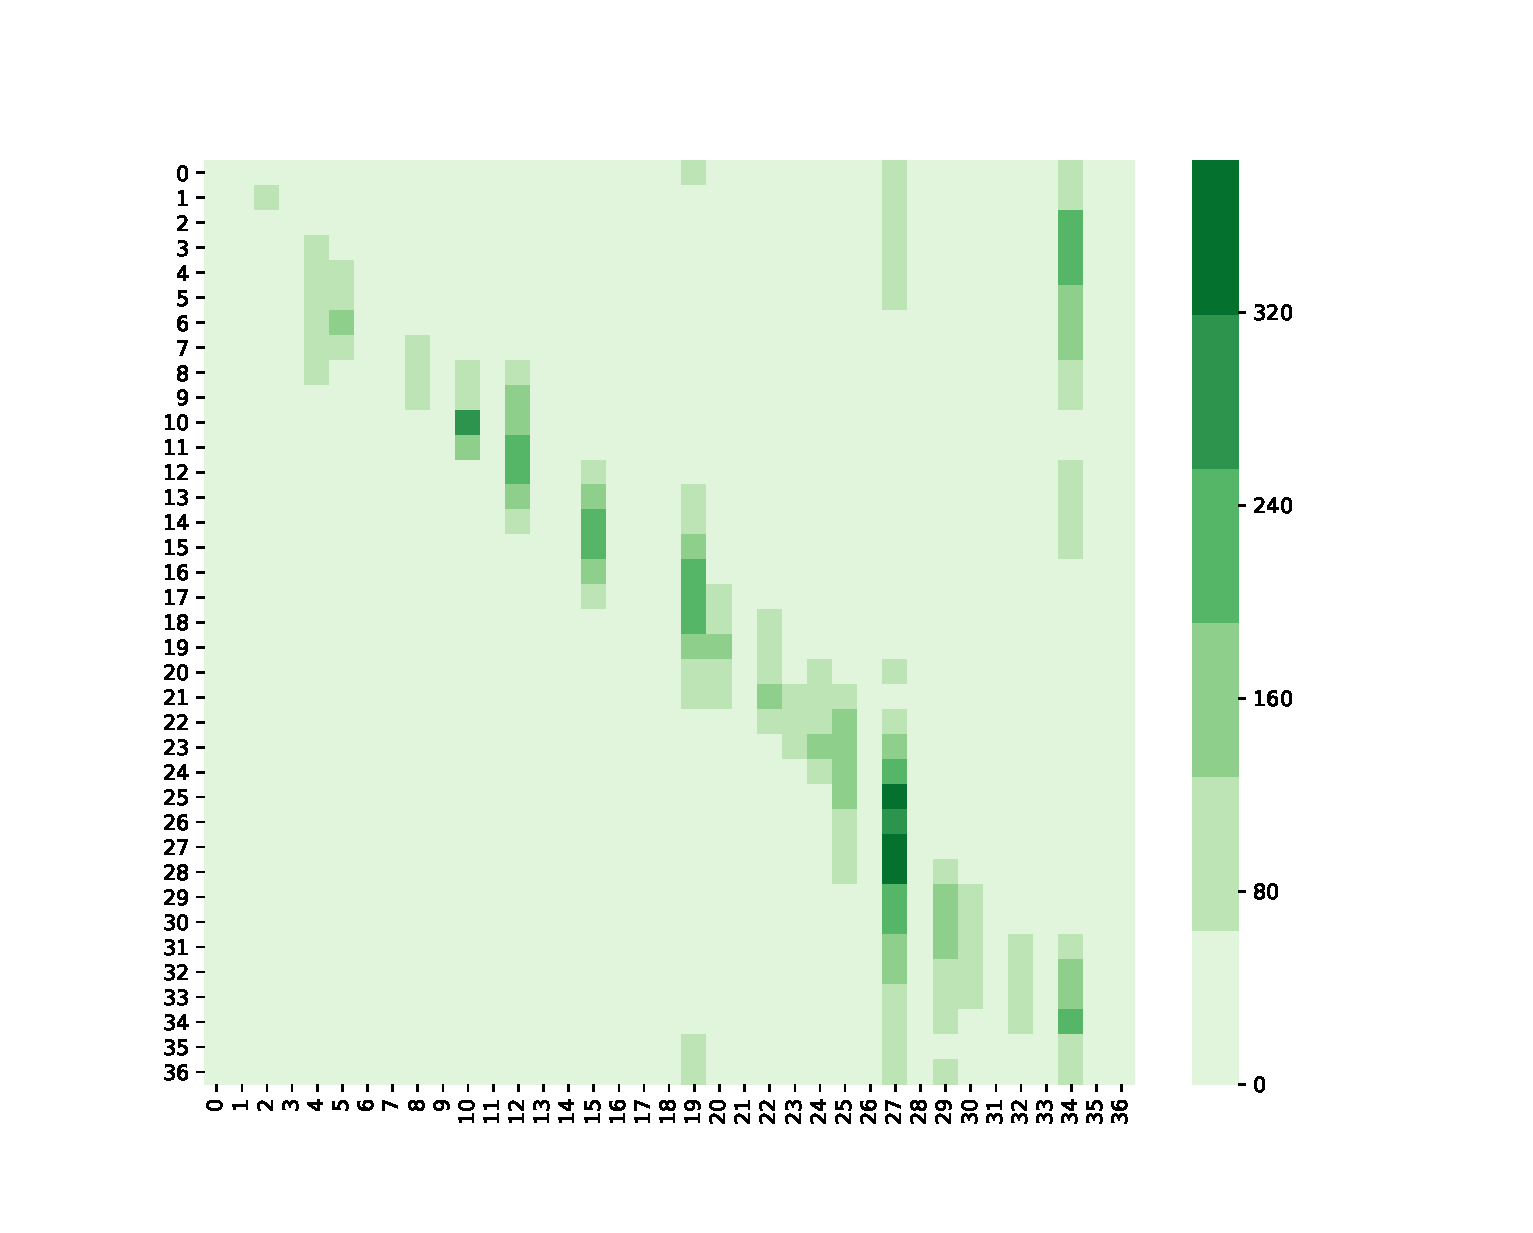
\includegraphics[width=\textwidth,height=\textheight,keepaspectratio]{Figures/confusion-matrix/ckpt-20622.eps}
        \caption[Confusion matrix obtained after 24 epochs of model training]
        {Confusion matrix obtained after 24 epochs of model training}
        \label{fig:cm-after-24-epochs}
    \end{minipage}

    \vspace*{1cm} % vertical separation

    \begin{minipage}{0.49\textwidth}
        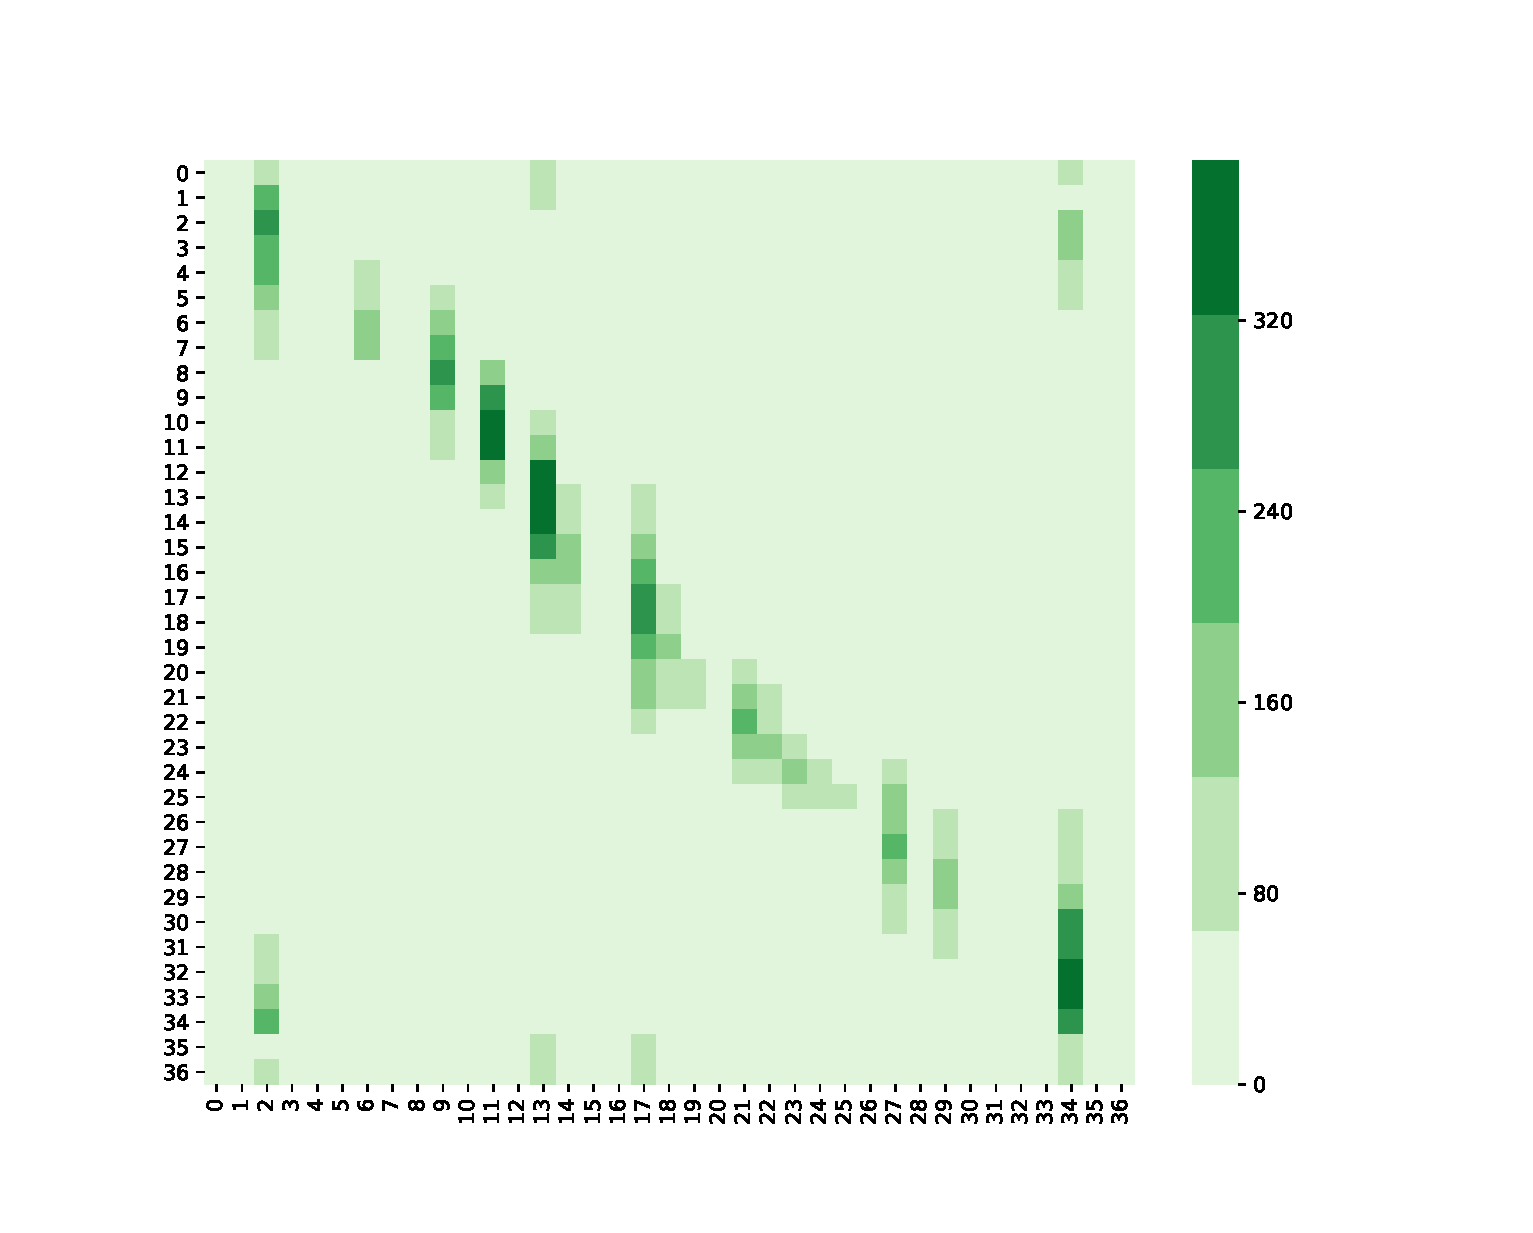
\includegraphics[width=\textwidth,height=\textheight,keepaspectratio]{Figures/confusion-matrix/ckpt-30757.eps}
        \caption[Confusion matrix obtained after 36 epochs of model training]
        {Confusion matrix obtained after 36 epochs of model training}
        \label{fig:cm-after-36-epochs}
    \end{minipage}
    \hspace{\fill} % note: no blank line here
    \begin{minipage}{0.49\textwidth}
        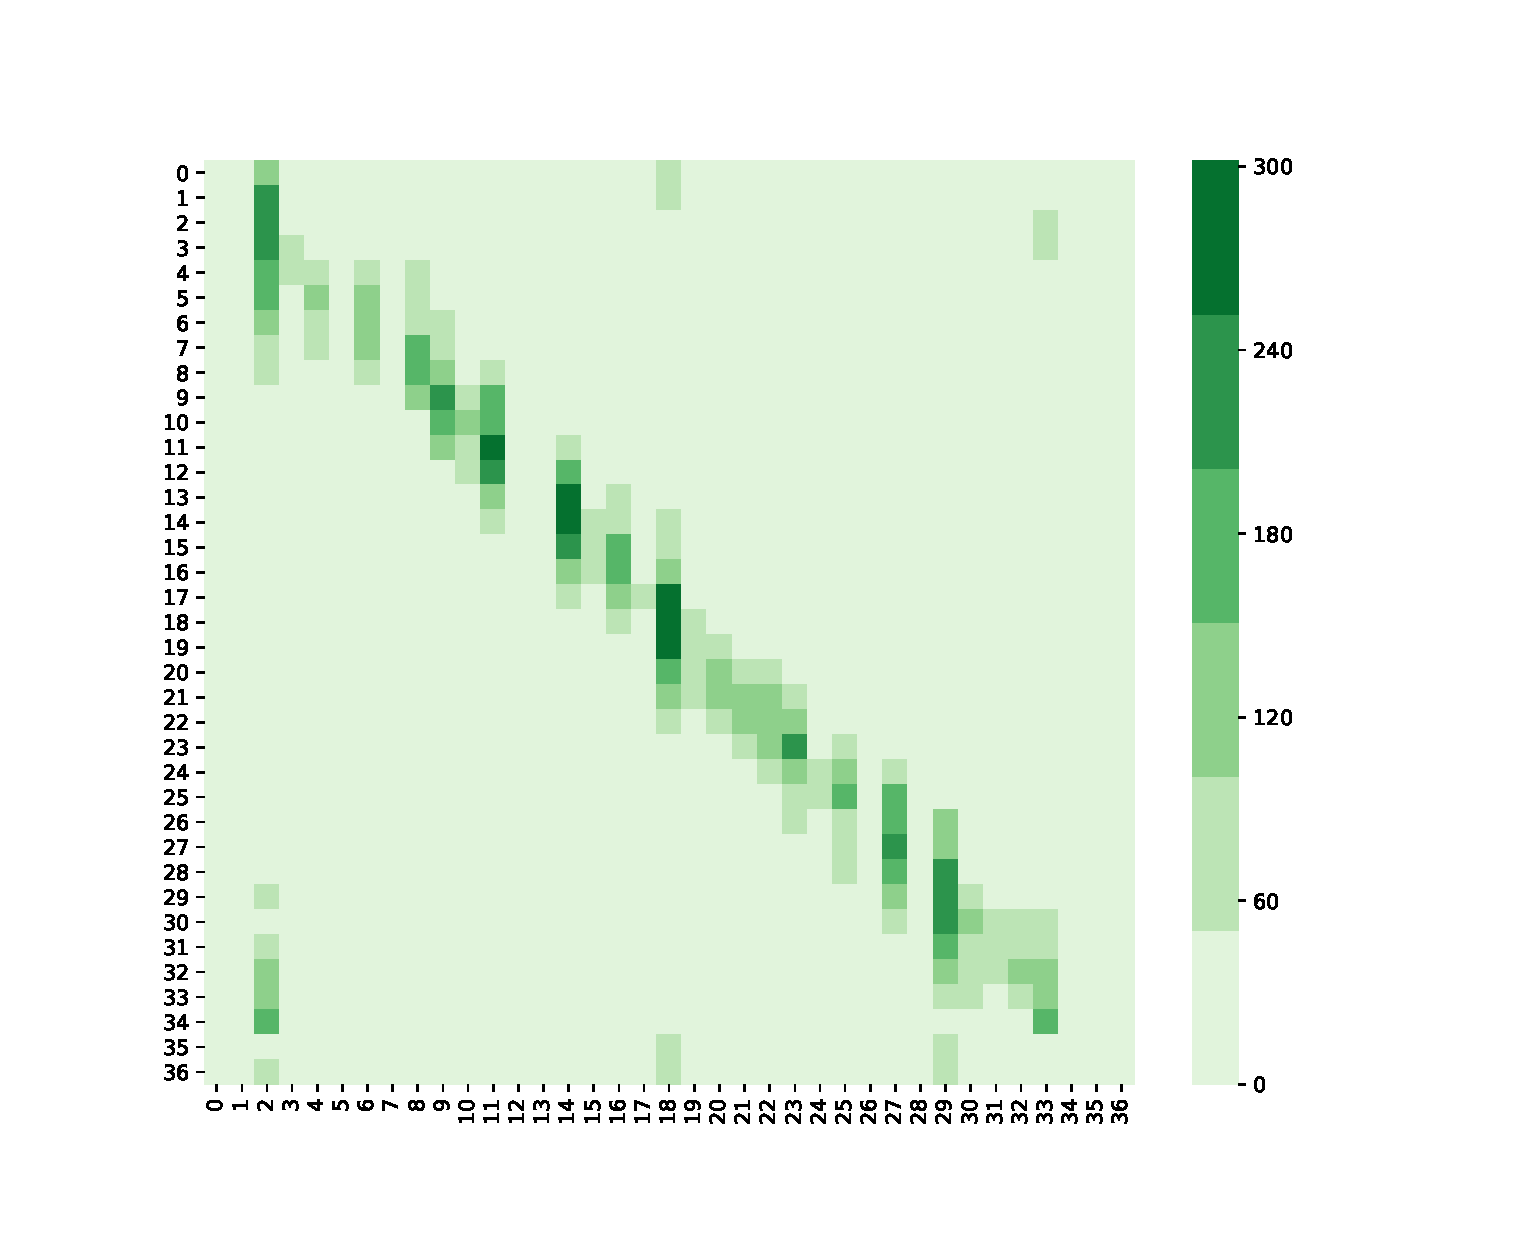
\includegraphics[width=\textwidth,height=\textheight,keepaspectratio]{Figures/confusion-matrix/ckpt-40884.eps}
        \caption[Confusion matrix obtained after 48 epochs of model training]
        {Confusion matrix obtained after 48 epochs of model training}
        \label{fig:cm-after-48-epochs}
    \end{minipage}
    % \caption{Figure caption goes here}\label{fig:see-data-visu}
\end{figure}
Confusion matrix~\parencite{RN216} is obtained after 
every validation process.
Figure~\ref{fig:cm-after-12-epochs},
Figure~\ref{fig:cm-after-24-epochs},
Figure~\ref{fig:cm-after-36-epochs}, and
Figure~\ref{fig:cm-after-48-epochs}
on page~\pageref{fig:cm-after-12-epochs}
show the confusion matrices
after 12, 24, 36 and 48 epochs of model training
separately.
The color thickness of block with coordinates $(i,j)$
expresses the frequency with which a block with best 
mode \emph{i} is predicted as \emph{j}.
For each horizontal line in the matrix, 
the probabilities of all blocks sum up to $100\%$.
From epoch 12 to epoch 48, most of the thicknesses 
in matrices have gradually been aggregated to 
the main diagonal, but there are nevertheless
four exceptional classes that predictions for them
have never been right in all the confusion matrices.
Those four classes are exactly mode DC, PLANAR, 
DMM1 and DMM4 which are tagged with mode index 
0, 1, 35 and 36 separately.
It turns out the neural networks will misclassify 
them into angular modes instead of giving 
predictions that are identical to their label 
of ground truth.
To cure this illness, it has been decided to
remove those four modes from target classes.

Different from the object recognition problems,
when convolutional neural networks are employed to 
predict the intra patterns, some popular data pre-processing
steps such as random crop, vertical flip
are not applicable anymore.
For example, angular mode 18 in Figure~\ref{fig:size8_mode18}
on page~\pageref{fig:size8_mode18} and angular mode 34 in
Figure~\ref{fig:size8_mode34} on page~\pageref{fig:size8_mode34}
would be identical to each other in terms of the edge angle
if either is vertically flipped.

Angular mode 2 and angular mode 34 are
on the same diagonal such that they cannot 
be taken as two separate classes in our case.
For this reason, it is decided to remove
blocks of angular mode 34
from the datasets.
Instead of directly predicting angular mode 34,
when the prediction result is angular mode 2,
there will be
a further comparison between mode 2 and mode 34 
using conventional encoder decision.

\section{Data Pre-processing}\label{sec:data-preprocessing}
According to the discussions in 
Subsection~\ref{subsec:discussion-about-data-visu}
on page~\pageref{subsec:discussion-about-data-visu},
which are based on the observations
of the visualized data in
Subsection~\ref{subsec:see-data-visu}
on page~\pageref{subsec:see-data-visu},
several pre-processing actions need
to be taken to clean up the collected data for deep learning.
The pre-processing steps are very crucial to the success
of the learning for the convolutional neural network.
Without pre-processing, it would be impossible
to achieve a satisfactory model performance 
for prediction tasks in our work.
In this section, the data pre-processing
are explained in details.

\begin{table}[H]
    % \begin{table}[!htbp]
    \caption{Information of the datasets after merging}
    \bigskip\label{tab:datasets-after-first-step}
    \centering
    \begin{tabular}{c c c c c}
        \toprule
        \# & Name of the file & Size & Samples & Usage\\
        \midrule
        1 & size04.csv & 206 MegaBytes & 3,675,428 & train,test,validate\\
        2 & size08.csv & 513 MegaBytes & 2,372,324 & train,test,validate\\
        3 & size16.csv & 1.25 GigaBytes & 1,439,773 & train,test,validate\\
        4 & size32.csv & 2.02 GigaBytes & 567,554 & train,test,validate\\
        \bottomrule
    \end{tabular}
\end{table}
Right after encoding four video sequences for data 
collection, four CSV files
would be obtained for each of them.
Every CSV file contains two unique identifications,
one is \emph{size of blocks}, the other is 
\emph{name of the source video sequence}.
For example, one of CSV files shall include depth 
Luma data of blocks of size \(16\times16\) from
\emph{Newspaper} video sequence.
In the first step of data-preprocessing, all
the CSV files having the same identification of 
\emph{size of blocks} shall be merged into a single dataset.
% which will be further divided into training dataset,
% testing dataset and validating dataset in the subsequent 
% processing steps.
The specifications of the four CSV files after merging 
are shown in Table~\ref{tab:datasets-after-first-step}
on page~\pageref{tab:datasets-after-first-step}.
There is no data for blocks of size \(64\times64\)
since the largest block size for DMM is \(32\times32\).
As the size of block
increases, the total volume of the collected data is growing
while the total number of samples of the collected data is
decreasing.
This phenomenon is reasonable in the sense that
the decreasing speed of the number of samples is slower 
than the increasing speed of the volume of every single
record.
More specifically, from block size \(4\times4\) to \(8\times8\),
the number of samples decreased by 1.55 times; however,
there is a fourfold increase of the volume size for 
each sample.

The statistics of the datasets after the first step of merging are
shown in Table~\ref{tab:unsorted-distribution-after-first-step}
on page~\pageref{tab:unsorted-distribution-after-first-step} and 
Table~\ref{tab:sorted-distribution-after-first-step}
on page~\pageref{tab:sorted-distribution-after-first-step}.
Each of them is unsorted or sorted in terms of the percentage
of each mode.
Each mode can be quickly found 
in Table~\ref{tab:unsorted-distribution-after-first-step}
on page~\pageref{tab:unsorted-distribution-after-first-step}
by looking at the first column.
From Table~\ref{tab:sorted-distribution-after-first-step}
on page~\pageref{tab:sorted-distribution-after-first-step},
it can be observed that the size differences of collected samples 
for each mode vary in a large range.
For example, the blocks of mode 0 are 96.9 times as many
the blocks of mode 16
while it is only 1.27 times as many the blocks of mode 35
for blocks of size \(32\times32\).
This is introducing the topic of imbalanced 
learning~\parencite{RN215} in which
the data size of each class can be very different.

According to the discussions presented in 
Subsection~\ref{subsec:discussion-about-data-visu},
mode 0, 1, 34, 35 and 36 will be removed from 
datasets in the second step.
The specifications of the data after the second step
are shown in Table~\ref{tab:datasets-after-second-step}.
More than half of the collected data are removed.
\begin{table}[H]
    % \begin{table}[!htbp]
    \caption{Information of the datasets after removing mode 0, 1, 34, 35 and 36}
    \bigskip\label{tab:datasets-after-second-step}
    \centering
    \begin{tabular}{c c c c c c}
        \toprule
        \# & Name of the file & Size & Samples & Usage & Percent of removed data (\%) \\
        \midrule
        1 & msize04.csv & 75.7 MegaBytes & 3,675,428 & train,test,validate & 64 \\
        2 & msize08.csv & 130.8 MegaBytes & 2,372,324 & train,test,validate & 74 \\
        3 & msize16.csv & 377.3 MegaBytes & 1,439,773 & train,test,validate & 70 \\
        4 & msize32.csv & 708.7 MegaBytes & 567,554 & train,test,validate & 65 \\
        % \# & Name of the file & Size & Samples & Usage\\
        % \midrule
        % 1 & msize04.csv & 75.7 MegaBytes & 3675428 & train,test,validate \\
        % 2 & msize08.csv & 130.8 MegaBytes & 2372324 & train,test,validate \\
        % 3 & msize16.csv & 377.3 MegaBytes & 1439773 & train,test,validate \\
        % 4 & msize32.csv & 708.7 MegaBytes & 567554 & train,test,validate \\
        \bottomrule
    \end{tabular}
\end{table}
In the third step, we start to remove the smooth blocks.
The reasons have been discussed in 
Subsection~\ref{subsec:discussion-about-data-visu}.
Algorithm~\ref{algo:edge-Sharpness} on page~\pageref{algo:edge-Sharpness},
which is based on the coarse edge sharpness analysis
in~\parencite{RN78}, has been designed to define the
sharpness of depth blocks.
%  as shown 

The difference between Algorithm~\ref{algo:edge-Sharpness}
and the coarse edge sharpness analysis in~\parencite{RN78}
is that the first one takes the average sharpness value
of top-k small square regions inside a single block as its
block sharpness while the second one sums all
the sharpness values of all small square regions inside a
single block as its sharpness.
In depth maps,
the sharpness typically is contributed by few sharp edges.
Lots of regions in a single sharp block are smooth regions.
Hence it makes sense to only evaluate the top-k average
instead of a sum of all.
An empirical threshold of \(15\) has been chosen to tag a block
as either smooth or sharp.
Blocks tagged with smooth will be removed from datasets
while the others will be kept.
The specifications of the data after the third step
of removing smooth blocks
are shown in Table~\ref{tab:datasets-after-third-step}.
Almost half of the data are removed.
\begin{table}[H]
    % \begin{table}[!htbp]
    \caption{Information of the datasets after removing smooth blocks}
    \bigskip\label{tab:datasets-after-third-step}
    \centering
    \begin{tabular}{c c c c c c}
        \toprule
        \# & Name of the file & Size & Samples & Usage & Percent of removed data (\%) \\
        \midrule
        1 & smsize04.csv & 36.3 MegaBytes & 616,281 & train,test,validate & 54 \\
        2 & smsize08.csv & 91.2 MegaBytes & 403,277 & train,test,validate & 33 \\
        3 & smsize16.csv & 210.9 MegaBytes & 232,806 & train,test,validate & 46 \\
        4 & smsize32.csv & 235.4 MegaBytes & 65,481 & train,test,validate & 79 \\
        \bottomrule
    \end{tabular}
\end{table}

The statistics of the datasets after the third step are
shown in Table~\ref{tab:unsorted-distribution-after-third-step}
on page~\pageref{tab:unsorted-distribution-after-third-step} and 
Table~\ref{tab:sorted-distribution-after-third-step}
on page~\pageref{tab:sorted-distribution-after-third-step}.
It is clear that after several pre-processing steps,
the issue of imbalanced learning~\parencite{RN215}
still exists.
To tackle the issue, we truncate datasets to make the
size of each class being equal.
In the last step, remaining 32 modes are tagged with integers
[0, 1, 2, \ldots, 31] to obtain new indices which
starting from zero for the convenience of deep learning.
At the same step, we separate datasets into training, 
testing and validating datasets.
Datasets for blocks of \(32\times32\) are too small
to be fed into the deep neural network.
They are consequently discarded.
The descriptions for the finalized datasets
are shown in Table~\ref{tab:finalized-four-by-four},
Table~\ref{tab:finalized-eight-by-eight}
and Table~\ref{tab:finalized-sixteen-by-sixteen}.
\begin{table}[H]
    % \begin{table}[!htbp]
    \caption{Information of the finalized datasets from blocks of size \(4\times4\)}
    \bigskip\label{tab:finalized-four-by-four}
    \centering
    \begin{tabular}{c c c c c}
        \toprule
        \# & Name of the file & Size & Samples & Usage\\
        \midrule
        1 & train04.csv & 7.9 MegaBytes & \(4,092\times32\) & train\\
        2 & test04.csv & 1.1 MegaBytes & \(600\times32\) & test\\
        3 & val04.csv & 1.1 GigaBytes & \(600\times32\) & validate\\
        \bottomrule
    \end{tabular}
\end{table}

\begin{table}[H]
    % \begin{table}[!htbp]
    \caption{Information of the finalized datasets from blocks of size \(8\times8\)}
    \bigskip\label{tab:finalized-eight-by-eight}
    \centering
    \begin{tabular}{c c c c c}
        \toprule
        \# & Name of the file & Size & Samples & Usage\\
        \midrule
        1 & train08.csv & 46.3 MegaBytes & \(6,303\times32\) & train\\
        2 & test08.csv & 3.8 MegaBytes & \(600\times32\) & test\\
        3 & val08.csv & 3.8 GigaBytes & \(600\times32\) & validate\\
        \bottomrule
    \end{tabular}
\end{table}

\begin{table}[H]
    % \begin{table}[!htbp]
    \caption{Information of the finalized datasets from blocks of size \(16\times16\)}
    \bigskip\label{tab:finalized-sixteen-by-sixteen}
    \centering
    \begin{tabular}{c c c c c}
        \toprule
        \# & Name of the file & Size & Samples & Usage\\
        \midrule
        1 & train16.csv & 89.9 MegaBytes & \(3,075\times32\) & train\\
        2 & test16.csv & 15.9 MegaBytes & \(600\times32\) & test\\
        3 & val16.csv & 15.9 GigaBytes & \(600\times32\) & validate\\
        \bottomrule
    \end{tabular}
\end{table}
%%%%%%%%%%%%%%%%%%%%%%%%%%%%%%%%%%%%%

\begin{algorithm}[!b]
    % \newcommand{\abs}[1]{\left|#1\right|}
    \SetKwData{FlattenLumaVals}{FlattenLumaVals}
    \SetKwData{SquareLumaVals}{SquareLumaVals}
    \SetKwData{TaggedMode}{TaggedMode}
    \SetKwData{HorSharpness}{HorSharpness}
    \SetKwData{VerSharpness}{VerSharpness}
    \SetKwData{Sharpness}{Sharpness}
    \SetKwData{TotalSharpness}{TotalSharpness}
    \SetKwData{ArrayOfSharpness}{ArrayOfSharpness}
    \SetKwData{ISSMOOTH}{ISSMOOTH}
    \SetKwData{BLKSIZE}{BLKSIZE}
    \SetKwData{SIZEOFARRAY}{SIZEOFARRAY}
    \SetKwData{BlockSharpness}{BlockSharpness}

    \SetKwFunction{getLength}{getLength}
    \SetKwFunction{reshape}{reshape}
    \SetKwFunction{pushValIntoArray}{pushValIntoArray}
    \SetKwFunction{sortArray}{sortArray}
    \SetKwFunction{getTopKEleAndFormNewArray}{getTopKEleAndFormNewArray}
    \SetKwFunction{removeEleLessThanEight}{removeEleLessThanEight}
    \SetKwFunction{getSizeOfArray}{getSizeOfArray}
    \SetKwFunction{getMeanOfArray}{getMeanOfArray}

    \DontPrintSemicolon% Some LaTeX compilers require you to use \dontprintsemicolon instead
    
    \KwIn{Luma pixel values stored inside an one dimensional array \FlattenLumaVals, 
    % label of ground truth \TaggedMode
    }
    \KwOut{Boolean value \ISSMOOTH}

    \Begin{
    
    \BLKSIZE\(\leftarrow\) \(|\sqrt{\getLength{\FlattenLumaVals}}|\)\;
    \SquareLumaVals\(\leftarrow\)\reshape{\FlattenLumaVals}\;
    \TotalSharpness\(\leftarrow0\)\;
    \ArrayOfSharpness\(\leftarrow\oldemptyset\)\;

    \For{\(i\leftarrow 0\) \KwTo \(\BLKSIZE-1\)}{
        \For{\(j\leftarrow 0\) \KwTo \(\BLKSIZE-1\)}{
            \HorSharpness\(x\leftarrow\)
            \SquareLumaVals[\(i\)][\(j\)] \(+\) 
            \SquareLumaVals[\(i+1\)][\(j\)] \(-\) 
            \SquareLumaVals[\(i\)][\(j+1\)] \(-\) 
            \SquareLumaVals[\(i+1\)][\(j+1\)]\;
            \VerSharpness\(x\leftarrow\)
            \SquareLumaVals[\(i\)][\(j\)] \(+\) 
            \SquareLumaVals[\(i\)][\(j+1\)] \(-\) 
            \SquareLumaVals[\(i+1\)][\(j\)] \(-\) 
            \SquareLumaVals[\(i+1\)][\(j+1\)]\;
            \Sharpness\(\leftarrow\HorSharpness^2 + \VerSharpness^2\)\;
            \TotalSharpness\(\leftarrow\TotalSharpness+\Sharpness\)\;
            \ArrayOfSharpness\(\leftarrow\) \pushValIntoArray{\ArrayOfSharpness, \Sharpness}\;
        }   
    }
    \ArrayOfSharpness\(\leftarrow\) \sortArray{\ArrayOfSharpness}\;
    \ArrayOfSharpness\(\leftarrow\) \getTopKEleAndFormNewArray{\ArrayOfSharpness, \(\BLKSIZE\times2\)}\;
    \ArrayOfSharpness\(\leftarrow\) \removeEleLessThanEight{\ArrayOfSharpness}\;
    \SIZEOFARRAY\(\leftarrow\) \getSizeOfArray{\ArrayOfSharpness}\;
    \eIf{\SIZEOFARRAY \(\equiv 0\)}{
    \BlockSharpness\(\leftarrow 0\)\;
    }{
    \BlockSharpness\(\leftarrow\) \getMeanOfArray{ArrayOfSharpness}\;
    }
    \eIf{\BlockSharpness \(> 15\)}{
    \ISSMOOTH\(\leftarrow 0\)
    }{
    \ISSMOOTH\(\leftarrow 1\)
    }
    }
 \caption{Sharpness analysis for single block}\label{algo:edge-Sharpness}
\end{algorithm}
%%%%%%%%%%%%%%%%%%%%%%%%%%%%%%%%%%%%%%%%%%%%%%%%

\begin{table}[H]
    % \begin{table}[!htbp]
    \caption{Unsorted statistics of datasets obtained after merging}
    \bigskip\label{tab:unsorted-distribution-after-first-step}
    \centering
    \resizebox{\textwidth}{!}
    {\begin{tabular}{c c c c c c c c c}
        \toprule
        Block Size & \multicolumn{2}{c}{\(4\times4\)} & \multicolumn{2}{c}{\(8\times8\)} & \multicolumn{2}{c}{\(16\times16\)} & \multicolumn{2}{c}{\(32\times32\)} \\
        Mode Idx & Samples & Percent (\%) & Samples & Percent (\%) & Samples & Percent (\%) & Samples & Percent (\%)\\
        \midrule
        0 & 717,274 & 19.52 & 642,520 & 27.08 & 459,291 & 31.90 & 158,824 & 27.98 \\ 
        1 & 482,776 & 13.14 & 249,061 & 10.50 & 164,050 & 11.39 & 57,528 & 10.14 \\ 
        2 & 97,629 &  2.66 & 25,101 &  1.06 & 12,868 &  0.89 & 4,561 &  0.80 \\ 
        3 & 17,991 &  0.49 & 12,489 &  0.53 & 7,946 &  0.55 & 2,863 &  0.50 \\ 
        4 & 14,375 &  0.39 & 11,688 &  0.49 & 8,642 &  0.60 & 2,175 &  0.38 \\ 
        5 & 15,849 &  0.43 & 13,428 &  0.57 & 8,829 &  0.61 & 2,164 &  0.38 \\ 
        6 & 17,144 &  0.47 & 15,318 &  0.65 & 9,768 &  0.68 & 2,958 &  0.52 \\ 
        7 & 18,187 &  0.49 & 17,238 &  0.73 & 15,988 &  1.11 & 6,625 &  1.17 \\ 
        8 & 19,146 &  0.52 & 15,785 &  0.67 & 20,357 &  1.41 & 11,642 &  2.05 \\ 
        9 & 23,462 &  0.64 & 12,362 &  0.52 & 18,207 &  1.26 & 18,195 &  3.21 \\ 
       10 & 42,752 &  1.16 & 9,740 &  0.41 & 7,978 &  0.55 & 18,972 &  3.34 \\ 
       11 & 23,727 &  0.65 & 12,836 &  0.54 & 17,696 &  1.23 & 21,142 &  3.73 \\ 
       12 & 21,992 &  0.60 & 17,837 &  0.75 & 23,143 &  1.61 & 13,262 &  2.34 \\ 
       13 & 24,613 &  0.67 & 20,254 &  0.85 & 19,260 &  1.34 & 6,740 &  1.19 \\ 
       14 & 22,620 &  0.62 & 17,784 &  0.75 & 13,851 &  0.96 & 2,995 &  0.53 \\ 
       15 & 21,169 &  0.58 & 18,268 &  0.77 & 12,834 &  0.89 & 2,073 &  0.37 \\ 
       16 & 20,289 &  0.55 & 15,418 &  0.65 & 10,214 &  0.71 & 1,639 &  0.29 \\ 
       17 & 21,869 &  0.60 & 17,501 &  0.74 & 10,010 &  0.70 & 1,977 &  0.35 \\ 
       18 & 52,552 &  1.43 & 19,889 &  0.84 & 9,862 &  0.68 & 1,998 &  0.35 \\ 
       19 & 23,871 &  0.65 & 16,171 &  0.68 & 9,797 &  0.68 & 2,170 &  0.38 \\ 
       20 & 22,992 &  0.63 & 15,656 &  0.66 & 10,227 &  0.71 & 1,925 &  0.34 \\ 
       21 & 25,416 &  0.69 & 16,706 &  0.70 & 11,978 &  0.83 & 2,504 &  0.44 \\ 
       22 & 27,593 &  0.75 & 16,446 &  0.69 & 12,251 &  0.85 & 2,925 &  0.52 \\ 
       23 & 33,250 &  0.90 & 16,783 &  0.71 & 12,744 &  0.89 & 3,707 &  0.65 \\ 
       24 & 40,677 &  1.11 & 17,262 &  0.73 & 12,257 &  0.85 & 4,457 &  0.79 \\ 
       25 & 36,018 &  0.98 & 13,841 &  0.58 & 7,812 &  0.54 & 5,123 &  0.90 \\ 
       26 & 404,933 & 11.02 & 70,417 &  2.97 & 30,896 &  2.15 & 17,897 &  3.15 \\ 
       27 & 48,843 &  1.33 & 17,062 &  0.72 & 12,205 &  0.85 & 7,414 &  1.31 \\ 
       28 & 34,217 &  0.93 & 24,051 &  1.01 & 16,725 &  1.16 & 6,169 &  1.09 \\ 
       29 & 37,756 &  1.03 & 23,486 &  0.99 & 15,647 &  1.09 & 5,436 &  0.96 \\ 
       30 & 30,910 &  0.84 & 20,972 &  0.88 & 12,782 &  0.89 & 3,945 &  0.69 \\ 
       31 & 35,102 &  0.95 & 20,499 &  0.86 & 13,331 &  0.93 & 3,475 &  0.61 \\ 
       32 & 25,756 &  0.70 & 18,811 &  0.79 & 12,254 &  0.85 & 3,289 &  0.58 \\ 
       33 & 33,270 &  0.91 & 19,088 &  0.80 & 11,943 &  0.83 & 3,526 &  0.62 \\ 
       34 & 73,107 &  1.99 & 31,114 &  1.31 & 15,848 &  1.10 & 5,382 &  0.95 \\ 
       35 & 789,662 & 21.48 & 710,089 & 29.93 & 299,368 & 20.79 & 126,427 & 22.28 \\ 
       36 & 276,639 &  7.53 & 139,353 &  5.87 & 70,914 &  4.93 & 23,450 &  4.13 \\ 
        \bottomrule
    \end{tabular}
    }
\end{table}

\begin{table}[H]
    % \begin{table}[!htbp]
    \caption{Sorted statistics of datasets obtained after merging}
    \bigskip\label{tab:sorted-distribution-after-first-step}
    \centering
    \resizebox{\textwidth}{!}
    {\begin{tabular}{c c c c c c c c c c c c c}
        \toprule
        Block Size & \multicolumn{3}{c}{\(4\times4\)} & \multicolumn{3}{c}{\(8\times8\)} & \multicolumn{3}{c}{\(16\times16\)} & \multicolumn{3}{c}{\(32\times32\)} \\
        Row idx  & Mode idx & Samples & Percent (\%) & Mode idx & Samples & Percent (\%) & Mode idx & Samples & Percent (\%) & Mode idx & Samples & Percent (\%)\\
        \midrule
        0 & 4  & 14,375 &  0.39 & 10  & 9,740 &  0.41 & 25  & 7,812 &  0.54 & 16  & 1,639 &  0.29 \\ 
        1 & 5  & 15,849 &  0.43 & 4  & 11,688 &  0.49 & 3  & 7,946 &  0.55 & 20  & 1,925 &  0.34 \\ 
        2 & 6  & 17,144 &  0.47 & 9  & 12,362 &  0.52 & 10  & 7,978 &  0.55 & 17  & 1,977 &  0.35 \\ 
        3 & 3  & 17,991 &  0.49 & 3  & 12,489 &  0.53 & 4  & 8,642 &  0.60 & 18  & 1,998 &  0.35 \\ 
        4 & 7  & 18,187 &  0.49 & 11  & 12,836 &  0.54 & 5  & 8,829 &  0.61 & 15  & 2,073 &  0.37 \\ 
        5 & 8  & 19,146 &  0.52 & 5  & 13,428 &  0.57 & 6  & 9,768 &  0.68 & 5  & 2,164 &  0.38 \\ 
        6 & 16  & 20,289 &  0.55 & 25  & 13,841 &  0.58 & 19  & 9,797 &  0.68 & 19  & 2,170 &  0.38 \\ 
        7 & 15  & 21,169 &  0.58 & 6  & 15,318 &  0.65 & 18  & 9,862 &  0.68 & 4  & 2,175 &  0.38 \\ 
        8 & 17  & 21,869 &  0.60 & 16  & 15,418 &  0.65 & 17  & 10,010 &  0.70 & 21  & 2,504 &  0.44 \\ 
        9 & 12  & 21,992 &  0.60 & 20  & 15,656 &  0.66 & 16  & 10,214 &  0.71 & 3  & 2,863 &  0.50 \\ 
       10 & 14  & 22,620 &  0.62 & 8  & 15,785 &  0.67 & 20  & 10,227 &  0.71 & 22  & 2,925 &  0.52 \\ 
       11 & 20  & 22,992 &  0.63 & 19  & 16,171 &  0.68 & 33  & 11,943 &  0.83 & 6  & 2,958 &  0.52 \\ 
       12 & 9  & 23,462 &  0.64 & 22  & 16,446 &  0.69 & 21  & 11,978 &  0.83 & 14  & 2,995 &  0.53 \\ 
       13 & 11  & 23,727 &  0.65 & 21  & 16,706 &  0.70 & 27  & 12,205 &  0.85 & 32  & 3,289 &  0.58 \\ 
       14 & 19  & 23,871 &  0.65 & 23  & 16,783 &  0.71 & 22  & 12,251 &  0.85 & 31  & 3,475 &  0.61 \\ 
       15 & 13  & 24,613 &  0.67 & 27  & 17,062 &  0.72 & 32  & 12,254 &  0.85 & 33  & 3,526 &  0.62 \\ 
       16 & 21  & 25,416 &  0.69 & 7  & 17,238 &  0.73 & 24  & 12,257 &  0.85 & 23  & 3,707 &  0.65 \\ 
       17 & 32  & 25,756 &  0.70 & 24  & 17,262 &  0.73 & 23  & 12,744 &  0.89 & 30  & 3,945 &  0.69 \\ 
       18 & 22  & 27,593 &  0.75 & 17  & 17,501 &  0.74 & 30  & 12,782 &  0.89 & 24  & 4,457 &  0.79 \\ 
       19 & 30  & 30,910 &  0.84 & 14  & 17,784 &  0.75 & 15  & 12,834 &  0.89 & 2  & 4,561 &  0.80 \\ 
       20 & 23  & 33,250 &  0.90 & 12  & 17,837 &  0.75 & 2  & 12,868 &  0.89 & 25  & 5,123 &  0.90 \\ 
       21 & 33  & 33,270 &  0.91 & 15  & 18,268 &  0.77 & 31  & 13,331 &  0.93 & 34  & 5,382 &  0.95 \\ 
       22 & 28  & 34,217 &  0.93 & 32  & 18,811 &  0.79 & 14  & 13,851 &  0.96 & 29  & 5,436 &  0.96 \\ 
       23 & 31  & 35,102 &  0.95 & 33  & 19,088 &  0.80 & 29  & 15,647 &  1.09 & 28  & 6,169 &  1.09 \\ 
       24 & 25  & 36,018 &  0.98 & 18  & 19,889 &  0.84 & 34  & 15,848 &  1.10 & 7  & 6,625 &  1.17 \\ 
       25 & 29  & 37,756 &  1.03 & 13  & 20,254 &  0.85 & 7  & 15,988 &  1.11 & 13  & 6,740 &  1.19 \\ 
       26 & 24  & 40,677 &  1.11 & 31  & 20,499 &  0.86 & 28  & 16,725 &  1.16 & 27  & 7,414 &  1.31 \\ 
       27 & 10  & 42,752 &  1.16 & 30  & 20,972 &  0.88 & 11  & 17,696 &  1.23 & 8  & 11,642 &  2.05 \\ 
       28 & 27  & 48,843 &  1.33 & 29  & 23,486 &  0.99 & 9  & 18,207 &  1.26 & 12  & 13,262 &  2.34 \\ 
       29 & 18  & 52,552 &  1.43 & 28  & 24,051 &  1.01 & 13  & 19,260 &  1.34 & 26  & 17,897 &  3.15 \\ 
       30 & 34  & 73,107 &  1.99 & 2  & 25,101 &  1.06 & 8  & 20,357 &  1.41 & 9  & 18,195 &  3.21 \\ 
       31 & 2  & 97,629 &  2.66 & 34  & 31,114 &  1.31 & 12  & 23,143 &  1.61 & 10  & 18,972 &  3.34 \\ 
       32 & 36  & 276,639 &  7.53 & 26  & 70,417 &  2.97 & 26  & 30,896 &  2.15 & 11  & 21,142 &  3.73 \\ 
       33 & 26  & 404,933 & 11.02 & 36  & 139,353 &  5.87 & 36  & 70,914 &  4.93 & 36  & 23,450 &  4.13 \\ 
       34 & 1  & 482,776 & 13.14 & 1  & 249,061 & 10.50 & 1  & 164,050 & 11.39 & 1  & 57,528 & 10.14 \\ 
       35 & 0  & 717,274 & 19.52 & 0  & 642,520 & 27.08 & 35  & 299,368 & 20.79 & 35  & 126,427 & 22.28 \\ 
       36 & 35  & 789,662 & 21.48 & 35  & 710,089 & 29.93 & 0  & 459,291 & 31.90 & 0  & 158,824 & 27.98 \\ 
      
        \bottomrule
    \end{tabular}
    }
\end{table}

\begin{table}[H]
    % \begin{table}[!htbp]
    \caption{Unsorted statistics of datasets obtained after removing smooth blocks}
    \bigskip\label{tab:unsorted-distribution-after-third-step}
    \centering
    \resizebox{\textwidth}{!}
    {\begin{tabular}{c c c c c c c c c}
        \toprule
        Block Size & \multicolumn{2}{c}{\(4\times4\)} & \multicolumn{2}{c}{\(8\times8\)} & \multicolumn{2}{c}{\(16\times16\)} & \multicolumn{2}{c}{\(32\times32\)} \\
        Mode Idx & Samples & Percent (\%) & Samples & Percent (\%) & Samples & Percent (\%) & Samples & Percent (\%)\\
        \midrule
        0 & 0 &  0.00 & 0 &  0.00 & 0 &  0.00 & 0 &  0.00 \\ 
        1 & 0 &  0.00 & 0 &  0.00 & 0 &  0.00 & 0 &  0.00 \\ 
        2 & 28,569 &  4.64 & 14,319 &  3.55 & 6,418 &  2.76 & 1,444 &  2.21 \\ 
        3 & 6,302 &  1.02 & 8,170 &  2.03 & 4,275 &  1.84 & 879 &  1.34 \\ 
        4 & 5,292 &  0.86 & 7,503 &  1.86 & 4,625 &  1.99 & 929 &  1.42 \\ 
        5 & 5,730 &  0.93 & 8,511 &  2.11 & 4,302 &  1.85 & 872 &  1.33 \\ 
        6 & 6,632 &  1.08 & 10,450 &  2.59 & 4,998 &  2.15 & 1,080 &  1.65 \\ 
        7 & 7,361 &  1.19 & 11,455 &  2.84 & 7,077 &  3.04 & 2,302 &  3.52 \\ 
        8 & 7,870 &  1.28 & 11,580 &  2.87 & 7,595 &  3.26 & 2,861 &  4.37 \\ 
        9 & 10,022 &  1.63 & 9,954 &  2.47 & 5,768 &  2.48 & 3,588 &  5.48 \\ 
       10 & 19,385 &  3.15 & 8,059 &  2.00 & 4,427 &  1.90 & 2,769 &  4.23 \\ 
       11 & 11,591 &  1.88 & 10,272 &  2.55 & 6,840 &  2.94 & 4,299 &  6.57 \\ 
       12 & 10,234 &  1.66 & 12,985 &  3.22 & 9,746 &  4.19 & 3,159 &  4.82 \\ 
       13 & 11,248 &  1.83 & 14,037 &  3.48 & 10,408 &  4.47 & 2,500 &  3.82 \\ 
       14 & 10,838 &  1.76 & 12,570 &  3.12 & 8,151 &  3.50 & 1,532 &  2.34 \\ 
       15 & 10,328 &  1.68 & 12,086 &  3.00 & 7,059 &  3.03 & 1,222 &  1.87 \\ 
       16 & 9,930 &  1.61 & 10,393 &  2.58 & 6,237 &  2.68 & 1,103 &  1.68 \\ 
       17 & 11,132 &  1.81 & 11,701 &  2.90 & 6,198 &  2.66 & 1,321 &  2.02 \\ 
       18 & 28,674 &  4.65 & 13,292 &  3.30 & 6,192 &  2.66 & 1,180 &  1.80 \\ 
       19 & 12,181 &  1.98 & 11,106 &  2.75 & 6,478 &  2.78 & 1,364 &  2.08 \\ 
       20 & 12,661 &  2.05 & 10,773 &  2.67 & 6,510 &  2.80 & 1,298 &  1.98 \\ 
       21 & 14,320 &  2.32 & 11,436 &  2.84 & 7,234 &  3.11 & 1,551 &  2.37 \\ 
       22 & 15,903 &  2.58 & 11,567 &  2.87 & 7,882 &  3.39 & 1,778 &  2.72 \\ 
       23 & 16,902 &  2.74 & 11,845 &  2.94 & 8,804 &  3.78 & 2,333 &  3.56 \\ 
       24 & 21,987 &  3.57 & 12,093 &  3.00 & 8,941 &  3.84 & 2,909 &  4.44 \\ 
       25 & 19,726 &  3.20 & 10,167 &  2.52 & 5,089 &  2.19 & 2,705 &  4.13 \\ 
       26 & 190,471 & 30.91 & 40,592 & 10.07 & 14,439 &  6.20 & 4,821 &  7.36 \\ 
       27 & 23,172 &  3.76 & 12,240 &  3.04 & 6,943 &  2.98 & 3,322 &  5.07 \\ 
       28 & 17,158 &  2.78 & 17,156 &  4.25 & 10,722 &  4.61 & 2,909 &  4.44 \\ 
       29 & 17,788 &  2.89 & 16,161 &  4.01 & 9,801 &  4.21 & 2,114 &  3.23 \\ 
       30 & 14,012 &  2.27 & 14,060 &  3.49 & 8,341 &  3.58 & 1,554 &  2.37 \\ 
       31 & 14,527 &  2.36 & 13,054 &  3.24 & 7,459 &  3.20 & 1,269 &  1.94 \\ 
       32 & 11,072 &  1.80 & 11,944 &  2.96 & 7,149 &  3.07 & 1,264 &  1.93 \\ 
       33 & 13,263 &  2.15 & 11,746 &  2.91 & 6,698 &  2.88 & 1,250 &  1.91 \\ 
       34 & 0 &  0.00 & 0 &  0.00 & 0 &  0.00 & 0 &  0.00 \\ 
       35 & 0 &  0.00 & 0 &  0.00 & 0 &  0.00 & 0 &  0.00 \\ 
       36 & 0 &  0.00 & 0 &  0.00 & 0 &  0.00 & 0 &  0.00 \\ 
        \bottomrule
    \end{tabular}
    }
\end{table}

\begin{table}[H]
    % \begin{table}[!htbp]
    \caption{Sorted statistics of datasets obtained after removing smooth blocks}
    \bigskip\label{tab:sorted-distribution-after-third-step}
    \centering
    \resizebox{\textwidth}{!}
    {\begin{tabular}{c c c c c c c c c c c c c}
        \toprule
        Block Size & \multicolumn{3}{c}{\(4\times4\)} & \multicolumn{3}{c}{\(8\times8\)} & \multicolumn{3}{c}{\(16\times16\)} & \multicolumn{3}{c}{\(32\times32\)} \\
        Row idx  & Mode idx & Samples & Percent (\%) & Mode idx & Samples & Percent (\%) & Mode idx & Samples & Percent (\%) & Mode idx & Samples & Percent (\%)\\
        \midrule
        0 & 0  & 0 &  0.00 & 0  & 0 &  0.00 & 0  & 0 &  0.00 & 0  & 0 &  0.00 \\ 
        1 & 1  & 0 &  0.00 & 1  & 0 &  0.00 & 1  & 0 &  0.00 & 1  & 0 &  0.00 \\ 
        2 & 34  & 0 &  0.00 & 34  & 0 &  0.00 & 34  & 0 &  0.00 & 34  & 0 &  0.00 \\ 
        3 & 35  & 0 &  0.00 & 35  & 0 &  0.00 & 35  & 0 &  0.00 & 35  & 0 &  0.00 \\ 
        4 & 36  & 0 &  0.00 & 36  & 0 &  0.00 & 36  & 0 &  0.00 & 36  & 0 &  0.00 \\ 
        5 & 4  & 5,292 &  0.86 & 4  & 7,503 &  1.86 & 3  & 4,275 &  1.84 & 5  & 872 &  1.33 \\ 
        6 & 5  & 5,730 &  0.93 & 10  & 8,059 &  2.00 & 5  & 4,302 &  1.85 & 3  & 879 &  1.34 \\ 
        7 & 3  & 6,302 &  1.02 & 3  & 8,170 &  2.03 & 10  & 4,427 &  1.90 & 4  & 929 &  1.42 \\ 
        8 & 6  & 6,632 &  1.08 & 5  & 8,511 &  2.11 & 4  & 4,625 &  1.99 & 6  & 1,080 &  1.65 \\ 
        9 & 7  & 7,361 &  1.19 & 9  & 9,954 &  2.47 & 6  & 4,998 &  2.15 & 16  & 1,103 &  1.68 \\ 
       10 & 8  & 7,870 &  1.28 & 25  & 10,167 &  2.52 & 25  & 5,089 &  2.19 & 18  & 1,180 &  1.80 \\ 
       11 & 16  & 9,930 &  1.61 & 11  & 10,272 &  2.55 & 9  & 5,768 &  2.48 & 15  & 1,222 &  1.87 \\ 
       12 & 9  & 10,022 &  1.63 & 16  & 10,393 &  2.58 & 18  & 6,192 &  2.66 & 33  & 1,250 &  1.91 \\ 
       13 & 12  & 10,234 &  1.66 & 6  & 10,450 &  2.59 & 17  & 6,198 &  2.66 & 32  & 1,264 &  1.93 \\ 
       14 & 15  & 10,328 &  1.68 & 20  & 10,773 &  2.67 & 16  & 6,237 &  2.68 & 31  & 1,269 &  1.94 \\ 
       15 & 14  & 10,838 &  1.76 & 19  & 11,106 &  2.75 & 2  & 6,418 &  2.76 & 20  & 1,298 &  1.98 \\ 
       16 & 32  & 11,072 &  1.80 & 21  & 11,436 &  2.84 & 19  & 6,478 &  2.78 & 17  & 1,321 &  2.02 \\ 
       17 & 17  & 11,132 &  1.81 & 7  & 11,455 &  2.84 & 20  & 6,510 &  2.80 & 19  & 1,364 &  2.08 \\ 
       18 & 13  & 11,248 &  1.83 & 22  & 11,567 &  2.87 & 33  & 6,698 &  2.88 & 2  & 1,444 &  2.21 \\ 
       19 & 11  & 11,591 &  1.88 & 8  & 11,580 &  2.87 & 11  & 6,840 &  2.94 & 14  & 1,532 &  2.34 \\ 
       20 & 19  & 12,181 &  1.98 & 17  & 11,701 &  2.90 & 27  & 6,943 &  2.98 & 21  & 1,551 &  2.37 \\ 
       21 & 20  & 12,661 &  2.05 & 33  & 11,746 &  2.91 & 15  & 7,059 &  3.03 & 30  & 1,554 &  2.37 \\ 
       22 & 33  & 13,263 &  2.15 & 23  & 11,845 &  2.94 & 7  & 7,077 &  3.04 & 22  & 1,778 &  2.72 \\ 
       23 & 30  & 14,012 &  2.27 & 32  & 11,944 &  2.96 & 32  & 7,149 &  3.07 & 29  & 2,114 &  3.23 \\ 
       24 & 21  & 14,320 &  2.32 & 15  & 12,086 &  3.00 & 21  & 7,234 &  3.11 & 7  & 2,302 &  3.52 \\ 
       25 & 31  & 14,527 &  2.36 & 24  & 12,093 &  3.00 & 31  & 7,459 &  3.20 & 23  & 2,333 &  3.56 \\ 
       26 & 22  & 15,903 &  2.58 & 27  & 12,240 &  3.04 & 8  & 7,595 &  3.26 & 13  & 2,500 &  3.82 \\ 
       27 & 23  & 16,902 &  2.74 & 14  & 12,570 &  3.12 & 22  & 7,882 &  3.39 & 25  & 2,705 &  4.13 \\ 
       28 & 28  & 17,158 &  2.78 & 12  & 12,985 &  3.22 & 14  & 8,151 &  3.50 & 10  & 2,769 &  4.23 \\ 
       29 & 29  & 17,788 &  2.89 & 31  & 13,054 &  3.24 & 30  & 8,341 &  3.58 & 8  & 2,861 &  4.37 \\ 
       30 & 10  & 19,385 &  3.15 & 18  & 13,292 &  3.30 & 23  & 8,804 &  3.78 & 24  & 2,909 &  4.44 \\ 
       31 & 25  & 19,726 &  3.20 & 13  & 14,037 &  3.48 & 24  & 8,941 &  3.84 & 28  & 2,909 &  4.44 \\ 
       32 & 24  & 21,987 &  3.57 & 30  & 14,060 &  3.49 & 12  & 9,746 &  4.19 & 12  & 3,159 &  4.82 \\ 
       33 & 27  & 23,172 &  3.76 & 2  & 14,319 &  3.55 & 29  & 9,801 &  4.21 & 27  & 3,322 &  5.07 \\ 
       34 & 2  & 28,569 &  4.64 & 29  & 16,161 &  4.01 & 13  & 10,408 &  4.47 & 9  & 3,588 &  5.48 \\ 
       35 & 18  & 28,674 &  4.65 & 28  & 17,156 &  4.25 & 28  & 10,722 &  4.61 & 11  & 4,299 &  6.57 \\ 
       36 & 26  & 190,471 & 30.91 & 26  & 40,592 & 10.07 & 26  & 14,439 &  6.20 & 26  & 4,821 &  7.36 \\  
      
        \bottomrule
    \end{tabular}
    }
\end{table}
